\documentclass[11pt,a4paper,titlepage,twoside,openright]{book}
% Use the UniMelb Dissertation Template
\usepackage{amsmath}
\usepackage{amsfonts}   % if you want the fonts
\usepackage{graphicx}%11111111111111111111111111111
\usepackage{tikz}%11111111111111111111111111111
%\usepackage[french]{babel}
\usepackage[english]{babel} 
\usepackage{float}%11111111111111111111111111111
\usepackage{lipsum,multicol}%11111111111111111111111111111
%\usepackage[numbers,sort]{natbib}
\usepackage{rotating}
\usepackage{amssymb}
\usepackage{xcolor}
\DeclareMathOperator*{\argmin}{arg~~min}
%\usepackage{style/uomthesis}
\usepackage{style/IEEEtrantools}
\usepackage{mathtools}%11111111111111111111111111111
\usepackage{xfrac}%11111111111111111111111111111
\usepackage{lettrine}
\usepackage{cases}
\usepackage{pdflscape}
\usepackage[hang,flushmargin]{footmisc}%11111111111111111111111111111
\usepackage{hyperref}
\usepackage[nottoc]{tocbibind}%11111111111111111111111111111
\usepackage{empheq}%11111111111111111111111111111
\usepackage{systeme}%11111111111111111111111111111
\usepackage{scalerel}%11111111111111111111111111111
\usepackage[usestackEOL]{stackengine}%11111111111111111111111111111
\usepackage{titlesec}%11111111111111111111111111111
\usepackage{algorithm}%11111111111111111111111111111
\usepackage{algpseudocode}%11111111111111111111111111111*
\usepackage{xcolor, soul}%11111111111111111111111111111
\usepackage{caption}%11111111111111111111111111111
%\usepackage[bottom]{footmisc}%11111111111111111111111111111
\usepackage{algorithmicx}%11111111111111111111111111111
\usepackage{multirow}
\usepackage{blindtext}
\usepackage{hyperref}
\usepackage{nameref}
\usepackage{subcaption}
\usepackage{url}
\usepackage{pdflscape}
\usepackage{afterpage}
\usepackage{capt-of}
\usepackage{enumitem}
\usepackage{soul}
\usepackage{setspace}
\usepackage{changepage}
\usepackage{fancyhdr}
%\usepackage{geometry}
\usepackage[a4paper, total={170mm,257mm}, outer=23mm, inner=27mm, top=35mm, bottom=30mm]{geometry}
\newcounter{mylabelcounter}


\makeatletter
\newcommand{\labelText}[2]{%
#1\refstepcounter{mylabelcounter}%
\immediate\write\@auxout{%
  \string\newlabel{#2}{{1}{\thepage}{{\unexpanded{#1}}}{mylabelcounter.\number\value{mylabelcounter}}{}}%
}%
}
\makeatother
%\usepackage{style/uomthesis}




\newcommand\abstractname{Abstract}  %%% here
\makeatletter
\if@titlepage
  \newenvironment{abstract}{%
      \titlepage
      \null
      \@beginparpenalty\@lowpenalty
      \begin{center}%
        {\bfseries \Huge\abstractname\vspace{-2mm}}
         \medskip\noindent \rule{\linewidth}{.5pt}
        \@endparpenalty\@M
      \end{center}}%
     {\par\vfil\null\endtitlepage}
\else
  \newenvironment{abstract}{%
      \if@twocolumn
        \section*{\abstractname}%
      \else
        \small
        \begin{center}%
          {\bfseries \Huge\abstractname\vspace{\z@}}
           \medskip\noindent \rule{\linewidth}{.5pt}
        \end{center}%
        \quotation
      \fi}
      {\if@twocolumn\else\endquotation\fi}
\fi
\makeatother








\newcommand\acknowname{Acknowledgements}  %%% here
\makeatletter
\if@titlepage
  \newenvironment{acknowledgements}{%
      \titlepage
      \null
      \@beginparpenalty\@lowpenalty
      \begin{center}%
        {\bfseries \LARGE\acknowname\vspace{-2mm}}
         \medskip\noindent \rule{\linewidth}{.5pt}
        \@endparpenalty\@M
      \end{center}}%
     {\par\vfil\null\endtitlepage}
\else
  \newenvironment{acknowledgements}{%
      \if@twocolumn
        \section*{\acknowname}%
      \else
        \small
        \begin{center}%
          {\bfseries \Huge\acknowname\vspace{\z@}}
           \medskip\noindent \rule{\linewidth}{.5pt}
        \end{center}%
        \quotation
      \fi}
      {\if@twocolumn\else\endquotation\fi}
\fi
\makeatother






 
\pagestyle{fancy}
\fancyhf{}
\fancyhead[EL]{\nouppercase\leftmark}
\fancyhead[OR]{\nouppercase\rightmark}
\fancyhead[ER,OL]{\thepage}
%\bibliographystyle{ieeetr} 

% \geometry{
% a4paper,
% total={170mm,257mm},
% outer=20mm,
% inner=30mm,
% top=25mm,
% bottom=30mm,
% }
% 


\newcommand\abstractname{Abstract}  %%% here

\errorcontextlines\maxdimen

% begin vertical rule patch for algorithmicx (http://tex.stackexchange.com/questions/144840/vertical-loop-block-lines-in-algorithmicx-with-noend-option)
\makeatletter
% start with some helper code
% This is the vertical rule that is inserted
    \newcommand*{\algrule}[1][\algorithmicindent]{\makebox[#1][l]{\hspace*{.5em}\thealgruleextra\vrule height \thealgruleheight depth \thealgruledepth}}%
% its height and depth need to be adjustable
\newcommand*{\thealgruleextra}{}
\newcommand*{\thealgruleheight}{.75\baselineskip}
\newcommand*{\thealgruledepth}{.25\baselineskip}

\makeatletter
\newcommand\footnoteref[1]{\protected@xdef\@thefnmark{\ref{#1}}\@footnotemark}


\newcommand{\algorithmfootnote}[2][\footnotesize]{%
  \let\old@algocf@finish\@algocf@finish% Store algorithm finish macro
  \def\@algocf@finish{\old@algocf@finish% Update finish macro to insert "footnote"
    \leavevmode\rlap{\begin{minipage}{\linewidth}
    #1#2
    \end{minipage}}%
  }%
}\\
\renewcommand{\floatpagefraction}{.9}

\newcount\ALG@printindent@tempcnta
\def\ALG@printindent{%
    \ifnum \theALG@nested>0% is there anything to print
        \ifx\ALG@text\ALG@x@notext% is this an end group without any text?
            % do nothing
        \else
            \unskip
            \addvspace{-1pt}% FUDGE to make the rules line up
            % draw a rule for each indent level
            \ALG@printindent@tempcnta=1
            \loop
                \algrule[\csname ALG@ind@\the\ALG@printindent@tempcnta\endcsname]%
                \advance \ALG@printindent@tempcnta 1
            \ifnum \ALG@printindent@tempcnta<\numexpr\theALG@nested+1\relax% can't do <=, so add one to RHS and use < instead
            \repeat
        \fi
    \fi
    }%
\usepackage{etoolbox}
% the following line injects our new indent handling code in place of the default spacing
\patchcmd{\ALG@doentity}{\noindent\hskip\ALG@tlm}{\ALG@printindent}{}{\errmessage{failed to patch}}
\makeatother

% the required height and depth are set by measuring the content to be shown
% this means that the content is processed twice
\newbox\statebox
\newcommand{\myState}[1]{%
    \setbox\statebox=\vbox{#1}%
    \edef\thealgruleheight{\dimexpr \the\ht\statebox+1pt\relax}%
    \edef\thealgruledepth{\dimexpr \the\dp\statebox+1pt\relax}%
    \ifdim\thealgruleheight<.75\baselineskip
        \def\thealgruleheight{\dimexpr .75\baselineskip+1pt\relax}%
    \fi
    \ifdim\thealgruledepth<.25\baselineskip
        \def\thealgruledepth{\dimexpr .25\baselineskip+1pt\relax}%
    \fi
    %\showboxdepth=100
    %\showboxbreadth=100
    %\showbox\statebox
    \State #1%
    %\State \usebox\statebox
    %\State \unvbox\statebox
    %reset in case the next command is not wrapped in \myState
    \def\thealgruleheight{\dimexpr .75\baselineskip+1pt\relax}%
    \def\thealgruledepth{\dimexpr .25\baselineskip+1pt\relax}%
}
% end vertical rule patch for algorithmicx






\DeclarePairedDelimiter\abs{\lvert}{\rvert}
\DeclarePairedDelimiter\norm{\lVert}{\rVert}\\


\algnewcommand{\IfThenElse}[3]{% \IfThenElse{<if>}{<then>}{<else>}
  \State \algorithmicif\ #1\ \algorithmicthen\ #2\  #3}
  
  
\newcommand{\myfrac}[3][0pt]{\genfrac{}{}{}{}{\raisebox{#1}{$#2$}}{\raisebox{-#1}{$#3$}}}
\newcommand*\circled[1]{\tikz[baseline=(char.base)]{
            \node[shape=circle,draw,inner sep=0.5pt] (char) {#1};}}
\newcommand{\vect}[1]{\mbox{\boldmath${#1}$}}%$
\DeclareMathOperator*{\argmax}{arg\,max}
%\frenchbsetup{StandardLists=true}

\newenvironment{rcases}
  {\left.\begin{aligned}}
  {\end{aligned}\right\rbrace}
  
\hypersetup{
colorlinks = true,
linkcolor  = black,
bookmarks  = true,
urlcolor   = blue,
citecolor  = blue,
}

\setcounter{secnumdepth}{4}
\setcounter{tocdepth}{4}

\titleformat{\paragraph}
{\normalfont\normalsize\bfseries}{\theparagraph}{1em}{}
\titlespacing*{\paragraph}
{0pt}{3.25ex plus 1ex minus .2ex}{1.5ex plus .2ex}



%\titlespacing*{\section}
%{0.5pt}{5.5ex plus 1ex minus .2ex}{5.3ex plus .2ex}
%\titlespacing*{\subsection}
%{0.5pt}{5.5ex plus 1ex minus .2ex}{5.3ex plus .2ex}
%\titlespacing*{\subsubsection}
%{0.5pt}{5.5ex plus 1ex minus .2ex}{5.3ex plus .2ex}
%\titlespacing*{\paragraph}
%{0.5pt}{5.5ex plus 1ex minus .2ex}{5.3ex plus .2ex}
% For drafts uncomment the following line
%\usepackage[light,timestamp,first]{draftcopy}

% Comment out the following line TO MARK blank pages with the 
% text "This page intentionally left blank."
% \newcommand{\markblankpages}{}

% Comment out the following line for the copy submitted to the library
\newcommand{\archivalpapernote}{}


\pdfminorversion=5
\pdfobjcompresslevel=4
% User defined commands
%%
%% VERSION HISTORY
%%    22 May 2006 - John Papandriopoulos - Original version
%%    12 Jul 2007 - John Papandriopoulos - Converted into template
%%

%%
%% Custom Hyphenations
%%

\hyphenation{cross-talk}

%%
%% Sample custom-configuration
%%
%%   You are encouraged to modify the following section with any of your
%%   own custom commands, packages, etc.
%%

%error 'You should modify this section and remove this error.'

% for URLs
\usepackage{url}

% AMS packages
%\usepackage{amsfonts}
\usepackage{amssymb}
\usepackage{amsmath}
\usepackage{amsthm}
\usepackage[mathscr]{eucal}
\usepackage{graphicx}
\usepackage{epsfig}
\renewcommand{\arraystretch}{1.8}
% Allow equations to break over pages...
\interdisplaylinepenalty=2500
% Command to stop equation breaks
% Note: enclose this in braces when used...
\newcommand{\donotsplitoverpages}{\interdisplaylinepenalty=10000}

% Graphics
% \ifx\pdftexversion\undefined
%  \usepackage[dvips]{graphicx}
% \else
%  \usepackage[pdftex]{graphicx}
% \fi

% Enable IEEE macros
\usepackage{IEEEtrantools}

% Use a plain bibliography style
%\bibliographystyle{plain}
% Use the IEEE bibliography style (sorted)
%\bibliographystyle{style/IEEEtrans}
\bibliographystyle{style/these}
% Use the IEEE bibliography style (unsorted; order of reference)
%\bibliographystyle{IEEEtran}

% For isolated bibliographies
\usepackage{bibunits}

\usepackage{color}
\usepackage[noadjust]{cite}
\usepackage{caption}

% For cool tables
\usepackage{array}
\usepackage{multirow}
% For subfigures
%\usepackage{subfig}
\usepackage{subfigure}

% For algorithms
%\usepackage{algorithm}
%\usepackage{algorithmic}

% For cases
\usepackage{sublabel}

% For theroem numbers having the chapter included
\usepackage{style/chngcntr}

% For cool theorem styles
%\usepackage[amsthm]{ntheorem}
%\theorembodyfont{\normalfont}

% Theorem definition
\newtheorem{theorem}{Theorem}
\counterwithin{theorem}{chapter}

% Corollary definition
\newtheorem{corollary}{Corollary}
\counterwithin{corollary}{chapter}

% Result definition
\newtheorem{result}{Result}
\counterwithin{result}{chapter}

% Lemma definition
\newtheorem{lemma}{Lemma}
\counterwithin{lemma}{chapter}

% Proposition definition
\newtheorem{proposition}{Proposition}
\counterwithin{proposition}{chapter}

% Definition definition!
\newtheorem{definition}{Definition}
\counterwithin{definition}{chapter}

% Remark definition (no counter?)
\newenvironment{remark}{\emph{Remark:~}}{}

% Fact definition (no counter?)
\newenvironment{fact}{\emph{Fact:~}}{}

% (Re)Set the figure path
\newcommand{\setfigurepath}[1]{%
\ifx\figurepath\undefined
	\newcommand{\figurepath}{#1}
\else
	\renewcommand{\figurepath}{#1}
\fi%
}

% Used in the continued list environment below
\newcounter{continuedlist}

% Continued list environment
\newenvironment{continuedlist}{%
	\begin{enumerate}%
		% Space out each item
		\setlength{\itemsep}{1.25em}%
		% Start the enumeration from the previous value
		\setcounter{enumi}{\value{continuedlist}} 
}{%
		% Save the counter to continue it later
		\setcounter{continuedlist}{\value{enumi}}%
	\end{enumerate}%
	%\vspace{1.25em}%
	\vspace{1em}%
}

% Spaced out list environment
\newenvironment{spacedoutlist}{%
	\begin{itemize}%
		% Space out each item
		\setlength{\itemsep}{1.25em}%
}{%
	\end{itemize}%
}




\begin{document}

	%%
	%% Front matter
	%%
	\begin{frontmatter}
		%\frontmatterheadings
%outer=23mm, inner=27mm	
\begin{adjustwidth}{-6mm}{-6mm}

		% Collect the dissertation information for the title page
		% *-----------------------------------------------------------*
% *         Page de Garde (basé sur le modèle UPMC)
% * Dernière modif le : 2012/02/13
% *-----------------------------------------------------------*
% * README: 
% *   - se compile avec pdflatex
% *   - l'entête de ce fichier sert pour générer une page
% *     unique. Ce texte latex peut s'inclure (partie comprise 
% *     entre les lignes et  ) dans un document existant.
% *-----------------------------------------------------------*

% - - - - - - - entête pour avoir une page unique 


% - - - - - - - début de la page 


\thispagestyle{empty}

%\includegraphics[scale=0.12]{upmc-logo.png}

{



%\vspace*{1cm}

\begin{center}
%{A dissertation submitted for the degree of}\\
{A dissertation submitted in partial fulfilment of the requirements for the degree of}\\

\vspace*{0.5cm}

\bf{{\Huge{Doctor of Philosophy}}}\\
\vspace{2mm}
\text{\normalfont\ \textit{\small{of the}}}\\
\vspace{1mm}
\Large{\bf Pierre \& Marie Curie University}\\
\vspace{-2mm}
\text{\normalfont\ \textit{\small{Sorbonnes Universit\'es, Universit\'e Pierre \& Marie Curie Paris VI}}}\\
\vspace{3mm}
\text{\normalfont\ \textit{\small{Doctoral school of Mechanical, Acoustic, Electronic and Robotic Sciences of Paris}}}\\
\vspace{-2mm}
\text{\normalfont\ \textit{\small{\'Ecole Doctorale de Sciences Mécanique, Acoustique, \'Electronique et Robotique de Paris}}}\\
\vspace{3mm}
\text{\normalfont\ \textit{\small{in}}}\\
\vspace{2mm}
\Large{\bf Robotics}

\vspace*{0.7cm}
\text{\normalfont\ \small{presented by}} \\

\vspace*{0.4cm}
{\huge {\bf Anis Meguenani}} \\



\vspace{0.2cm}
\hrulefill \\
{\huge {\bf  Safe Control of Robotic Manipulators in Dynamic Contexts \\ }}
\hrulefill \\
\vspace{0.2cm}
\text{\normalfont\ \textit{\small{Defended on the $13^{th}$ of October, 2017}}}\\

\end{center}

\vspace*{0.8cm} 


\begin{center}
\Large{\bf Committee}\\
\vspace{0.5cm}
\begin{small}
{\def\arraystretch{1.3}\tabcolsep=5pt
\begin{tabular}{lll}
\vspace{2mm}
M. Olivier {\sc STASSE} & Senior Researcher at LAAS-CNRS, Toulouse & Referee \\
\vspace{2mm}
M. Sami {\sc HADDADIN} & Research director at Leibniz Universit\"at, Hannover & Referee  \\
\vspace{2mm}
M. Guillaume {\sc MOREL} & Professor at Universit\'e Pierre \& Marie Curie    & Examiner  \\
\vspace{2mm}
M. Andrea {\sc DEL PRETE} & Post Doc at LAAS-CNRS, Toulouse  & Examiner  \\
\vspace{2mm}
M. Yvan {\sc MEASSON}  & CEO at ISYBOT, Gif-Sur-Yvette  & Guest member \\
\vspace{2mm}
M. Philippe {\sc BIDAUD}    & Professor at Universit\'e Pierre \& Marie Curie  & Adviser  \\
\vspace{2mm}
M. Vincent  {\sc PADOIS}     & Associate professor at Universit\'e Pierre \& Marie Curie  & Adviser \\


\end{tabular}%
}
\end{small}
\end{center}



}
% - - - - - - - fin de la page 






		\cleardoublepage
		
		% Generate the title page
		%\maketitle

		% Author declaration
		%\makedeclaration
\end{adjustwidth}	
		% Acknowledgements
		%%
%% VERSION HISTORY
%%    22 May 2006 - John Papandriopoulos - Original version
%%    12 Jul 2007 - John Papandriopoulos - Converted into template
%%
\begin{acknowledgements}
Foremost, I would like to express my sincere gratitude to my two supervisors Prof. Philippe Bidaud and Prof. Vincent Padois for giving me the opportunity to be part of the \textit{Institut des syst\`emes intelligents et de robotique} (ISIR), for their continuous support during my Ph.D study and research, for their patience, motivation, enthusiasm, trust and immense knowledge. Their guidance made it possible to achieve the goals fixed for my thesis and also to write this report. \\
% it was impossible to reach the goal
%it has been a honour to be her their Ph.D. student.
%
%me during all the time of research and writing of this thesis and i could not have imagined having better advisors and mentors.  \\

Additionally, i would like to thank my committee members Dr. Olivier Stasse, Prof. Sami Haddadin, Prof. Guillaume Morel, Dr. Andrea Del Prete and Dr. Yvan Measson for their interest in my work. \\

I am also thankful to my colleagues Zhanat Kappassov, Ziad Zamzami, Mohammed Fnadi, Pauline Maurice, Ryan Lober, Mingxing Liu, Darwin Lau, Aurélien Ibanez, Philipp Schlehuner and Jorhabib Eljaik Gomez for their friendship, support, and for creating a cordial working environment. I would like also to thank Sovannara Hak, Antoine Hoarau and Jimmy Da Silva for their valuable help and technical assistance for the experimentations performed on the KUKA LWR4 robot. \\

Finally, in the pursuit of this Ph.D, the members of my family have been of great importance to me. More specifically, i would like to thank my mother Assia Meguenani and father Saadoun Meguenani for their unconditional love and moral and emotional support throughout my life and for making of me the person i am today. 

%Finally, nobody has been more important to me in the pursuit of this Ph.D than the members of my family. More specifically, i would like to thank my mother Assia Meguenani and father Saadoun Meguenani for their unconditional love and moral and emotional support throughout my life and for making of me the man i am today.
%
%Three year PhD experience is unforgettable and enjoyable for me. I am happy that I have learned many things concerning my research topics, the way to work, and the skills to live abroad. At the end of this journey, I would like to sincerely thank all the people who have been in my life and supporting me.
%
%First of all, I would like to thank my supervisor Prof. Philippe Bidaud for giving the opportunity to study at Pierre and Marie Currie University in France. I cherish this studying opportunity abroad. Not only because I can understand French customs and cultures, but also I can work in the institute for intelligent systems and robotics (ISIR), one of most famous robotic laboratory in the world. I would also like to thank Prof. Vincent Padois, who have provided me with his valuable time, patience and experience whenever it was needed. In addition to his guidance towards my PhD research, Vincent is like a friend. I also thank him for his nurturing to prepare me for the future with valuable life attitudes. 
%
%Secondly, appreciation goes to my colleagues in ISIR. I would like to thank Mingxing Liu and Darwin Lau for their inspiring discussions on robotics and their insightful comments on my research work. I would also like to thank Joseph Sainili, Sovannara Hak, Aurélien Ibanez, Pauline Maurice, Anis Meguenani, Ryan Lober, Tianming Lu, and Munan Yin for their ongoing support and advice both in and out of my research.
%
%
%Finally, I must acknowledge and thank my family. Thanks to my wife Dongya Liu for being with me and encouraging me during this challenging journey. I would also like to thank my parents, Zhizhong Tan and Yonghua Yang, for their everlasting love and support throughout my life. 
\end{acknowledgements}

		\begin{abstract}
{\setstretch{1.0}
\vspace{3mm}
The intended goal of this thesis is to bring new insights for developing robotic systems capable of safely sharing their workspace with human-operators. Within this context, the presented work focuses on the control problem. The following questions are tackled:
\begin{itemize}
\item for reactive control laws, i.e., control problems where the task to be performed is not known in advance but discovered \textit{on-line}, how is it possible to guarantee for every time-step the existence of a solution to the control problem? This solution should allow the robot to accomplish at best its prescribed task and at the same time to strictly comply with existing constraints, among which, constraints related to the physical limitations of its actuators and joints.
\item How to integrate the human-operator in the control loop of the robot so that physical contact can safely  be engaged and de-engaged?
\end{itemize}
Regarding the first point, our work arises as the continuity of previous results developed by S\'ebastien Rubrecht during his PhD thesis. S\'ebastien Rubrecht introduced the concept of \textit{constraints incompatibility} for robots reactively controlled at the kinematic-level. The problem of \textit{constraints incompatibility} appears for example when the formulation of the constraint on an articular position of a robot does not account for the amount of deceleration producible by its actuator. In such case, if the articular position constraint is activated tardively, the system may not have sufficient time to cope with the imposed joint position limit considering its bounded dynamic capabilities. \\
In our work, the problem of \textit{constraints incompatibility} is tackled for robots controlled at the dynamic-level (torque control). New mathematical formulations for the \textit{articular position} and \textit{joint velocity} constraints that account for both the deceleration and jerk capabilities of the actuators of the robot are introduced. The \textit{optimal} time needed for the system to cope with the different limits of these constraints is computed. When included in a QP formulation of the control problem, the introduced new expressions trigger the activation of the constraints at the right time considering the dynamic capabilities of the robot. The existence of a constraint compliant and optimal solution as joint position, velocity, torque/deceleration and also jerk limits are all respected at the same time and at every time-step is guaranteed. Consequently the \textit{viability} of the state of the robot is also ensured.

Regarding the second point, for a given shape of the robot, two main parameters are usually considered for safety: the impact force generated at collision and the contact force generated after the establishment of physical contact. The most generic way to consider and express these parameters is to use an energetic formulation of the safety problem. Indeed, energy is a universal quantity that can describe all the safety related physical phenomena occurring during human-robot interaction. An impact force for example is directly proportional to the amount of kinetic energy dissipated at collision. The contact force on the other hand derives from the amount of potential energy that accumulates in the controller of the robot during physical contact. In our work, safety during human-robot interaction is handled by modulating the amount of energy instantaneously displayed by the robot. The main contributions are as follows:
\begin{itemize}
\item the formulation of kinetic and potential energy based safety indicators that represent the degree of danger of the robot at collision and during physical contact.
\item The formulation of energy based safety criteria that bound the dynamics of the robot during different interaction phases: at the approach of the human-operator, at collision, during physical contact and finally when contact is released.
\item The expression of the introduced indicators and criteria as inequality constraints related to the torque control input of a robotic manipulator.
\item The introduction of the concept of ``task energy profile'' to track the amount of energy used to accomplish a considered repetitive task in the most optimal way. This profile is then used to formulate a constraint on the instantaneous amount of energy the robot is allowed to exhibit at every time-step. When implemented in the control scheme, the ``task energy profile'' related constraint makes the robot comply to any deliberate or non-deliberate contact with its environment. 
\end{itemize}
For the validation of the proposed algorithms, beyond the theoretical contributions, simulation and experimental applications are performed on a KUKA LWR4 robotic manipulator.}
%Large and sudden changes in the torques of the actuators of a robot are highly undesirable and should be avoided during robot control as they may result in unpredictable behaviours. Multi-objective control system for complex robots usually have to handle multiple prioritized tasks while satisfying constraints. Changes in tasks and/or constraints are inevitable for robots when adapting to the unstructured and dynamic environment, and they may lead to large sudden changes in torques. Within this work, the problem of task priority transitions and changing constraints is primarily considered to reduce large sudden changes in torques. This is achieved through two main contributions as follows.
%
%Firstly, based on quadratic programming (QP), a new controller called Generalized Hierarchical Control (GHC) is developed to deal with task priority transitions among arbitrary prioritized task. This projector can be used to achieve continuous task priority transitions, as well as insert or remove tasks among a set of tasks to be performed in an elegant way. The control input (\textit{e.g.} joint torques) is computed by solving one quadratic programming problem, where generalized projectors are adopted to maintain a task hierarchy while satisfying equality and inequality constraints.
%
%Secondly, a predictive control primitive based on Model Predictive Control (MPC) is developed to handle presence of discontinuities in the constraints that the robot must satisfy, such as the breaking of contacts with the environment or the avoidance of an obstacle. The controller takes the advantages of predictive formulations to anticipate the evolutions of the constraints by means of control scenarios and/or sensor information, and thus generate new continuous constraints to replace the original discontinuous constraints in the QP reactive controller. As a result, the rate of change in joint torques is minimized compared with the original discontinuous constraints. This predictive control primitive does not directly modify the desired task objectives, but the constraints to ensure that the worst case of changes of torques is well-managed.
%
%The effectiveness of the proposed control framework is validated by a set of experiments in simulation on the Kuka LWR robot and the iCub humanoid robot. The results show that the proposed approach significantly decrease the rate of change in joint torques when task priorities switch or discontinuous constraints occur. 
\vspace{7mm}

\textbf{Keywords:} \textit{Redundant Robots, Dynamic Control, Safe Human-Robot Interaction, Kinetic energy, Potential Energy, Energy-Based Constraints.}
\end{abstract}

%robots redondants, contrôle dynamique, Commande prédictive, Optimisation quadratique, commande en couple, continuités des contraintes



		% Preface
		%%%
%% VERSION HISTORY
%%    22 May 2006 - John Papandriopoulos - Original version
%%    12 Jul 2007 - John Papandriopoulos - Converted into template
%%

% If applicable, a Preface includes where appropriate, a statement of:
% 
%    * work carried out in collaboration indicating the nature and proportion 
% 	 of the contribution of others and in general terms the portions of the
% 	 work which the candidate claims as original,
%    * work submitted for other `qualifications',
%    * work carried out prior to PhD candidature enrolment,
%    * any third party editorial assistance, either paid or voluntary (as 
% 	 limited to the Editing of Research Theses by Professional Editors 
% 	 guidelines) and/or
%    * where a substantially unchanged multi-author paper is included in the
% 	 thesis a statement prepared by the candidate explaining the 
% 	 contributions of all involved. A signed copy by all authors must be 
% 	 included with the submission form.


% Optional preface to the dissertation
\begin{preface}

	An preface can be written in \texttt{preface.tex}.

\end{preface}



		% Dedications...
		%% A personal dedication, it needn't be academically relevant
\begin{dedication}
	To the keys that always push back. 
\end{dedication}


		% Table of Contents, List of Figures, List of Tables
		%\singlespacing
		\tableofcontents

		%\listoffigures
		% Do not include a list of tables if you have less
		% than 10 tables, as per SGS suggestion.
%		\listoftables
		\clearpage
	\end{frontmatter}

	%\begin{nomenclature}

{\huge Acronyms}

\begin{table}[ht]
	\begin{center}
		\begin{tabular}{l l}
			PSO  & particle swarm optimisation (/optimiser)\\
		\end{tabular}
	\end{center}
\end{table}

\clearpage

{\huge Mathematical notations}

\begin{table}[ht]
	\begin{center}
		\begin{tabular}{l l}
			$t$				& time (s)\\
			$\dot{m}$		& mass flow rate (kg / s)\\
			$\nu$			& efficiency
		\end{tabular}
	\end{center}
\end{table}

\end{nomenclature}

	%%
	%% Main matter
	%%

 
	\begin{mainmatter}
%	\mainmatterheadings


		
%	\setlength{\belowdisplayskip}{14pt}
%    \setlength{\belowdisplayshortskip}{14pt}
%    \setlength{\abovedisplayskip}{14pt}
%    \setlength{\abovedisplayshortskip}{14pt}	
		
	%\chapter{Introduction}
\label{chap:intro}
\setfigurepath{figures/Intro}
%=========================================================================
%The intended goal of this thesis is to bring new insights for developing robotic systems capable of safely sharing their workspace with human operators. Within this context, the presented work focuses on the control problem. The following questions are tackled:
%1) for reactive control problems, i.e. control problems where the task to be performed is not known in advance but discovered on-line, how is it possible to guarantee at every time-step the existence of a solution to the control problem? This solution should allow the robot to accomplish at best its prescribed task and at the same time to strictly comply with existing constraints, among which, constraints related to the physical limitations of its actuators and joints.
%2) How to integrate the human operator within the control loop of the robot so that physical contact can be safely engaged and de-engaged?
%Regarding the first point, our work arises as the continuity of previous results developed by Sébastien Rubrecht during his PhD thesis.
%Sébastien Rubrecht introduced the concept of constraints incompatibility that appears for example when the formulation of an articular position related constraint does not take into account the amount of deceleration producible by the joint actuator. In this case, if this constraint is activated tardively, the system may not be able to cope with its position limit considering its bounded reaction capability. In his thesis, Rubrecht solved this problem for a robot reactively controlled at the kinematic level. In our work, the problem of constraints incompatibility is extended to robots controlled at the dynamic level. New mathematical formulations for the joint position and velocity constraints are introduced considering both the deceleration and jerk capabilities of the robot actuators. When included in a QP formulation of the control problem, these new expressions guarantee the existence of a constraint compliant and optimal solution at all time as joint position, velocity, torque/deceleration and also jerk limits are all respected at the same time and at every time-step.
%6:06
%Regarding the second point: for a given shape of the robot, two main parameters are usually considered for safety: the impact force generated at collision and the contact force generated after the establishment of physical contact. The most generic way to consider and express these parameters is to use an energetic formulation. Indeed, energy is a universal entity that can describe all physical phenomena occurring during human-robot interaction. An impact force for example is directly proportional to the amount of kinetic energy dissipated at collision. The contact force on the other hand derives from the amount of potential energy generated within the human-robot system during physical contact. In our work, safety during human-robot interaction is guaranteed by modulating the amount of energy instantaneously deployed by the robot. The main contributions are as following:
%1) the formulation of kinetic and potential energy based safety indicators that represent the degree of danger of the robot at collision and during physical contact.
%2) The formulation of safety criteria that bounds the dynamic of the robot during different interaction phases: at the approach of the human operator, at collision, during physical contact and finally when this contact is released.
%3) The expression of these indicators and criteria as inequality constraints related to the torque control input of a robotic arm.
%4) The introduction of the concept of "task energy profile" to track the amount of energy used to accomplish a considered repetitive task in the most optimal way. This profile is used to constrain the instantaneous amount of energy the robot is allowed to exhibit at every time-step.
%The resulting controller renders the robot compliant to any deliberate or non-deliberate contact with its environment.
%For the validation of the proposed algorithms, beyond the theoretical contributions, simulation and experimental applications are performed on a Kuka LWR-4 serial robot. 
\section{Motivation}
The present thesis is partially supported by the RTE company through the RTE/UPMC Chair of ``\textit{Intervention Robotics}" held by Vincent Padois. The intended goal of this chair is to bring new insights for the development of intervention robotic systems and assistant robots capable of safely interacting with human operators. Within this context, the work presented hereby focuses on the control problem. M\'ecaniques \\
Domains of application for robots are evolving from purely structured industrial contexts to the human world as intervention machines and assistants to aid humans in the completion of manual tasks. This has a direct impact on the formulation of the control problem that must be completely reconsidered. Indeed, when industrial robots are aimed for tasks that are relatively simple (e.g. \textit{pick and place manipulation}), repetitive, within perfectly known static and protected environments; Service and collaborative robots are confronted to more challenging scenarios: unknown, constrained and dynamic environments with possible deliberate and non deliberate interactions with humans. 
\section{Research questions and contributions}
The goal of the presented work is to seek answers for the following questions: 
\begin{itemize}
\item For reactive control problems, i.e. control problems where the task to be performed is not known in advance but discovered on-line, how is it possible to guarantee every time-step the existence of a solution to the control problem ? This solution should allow the robot to accomplish at best its prescribed task and at the same time to strictly comply with existing constraints, among which, constraints related to the physical limitations of its actuators and joints.
\item How to integrate the human operator within the control loop of the robot so that physical contact can be safely engaged and de-engaged ? 
\end{itemize} 
Regarding the first point, our work arises as the continuity of previous results developed by Sébastien Rubrecht during his PhD thesis.
Sébastien Rubrecht introduced the concept of constraints incompatibility that appears for example when the formulation of an articular position related constraint does not take into account the amount of deceleration producible by the joint actuator. In this case, if this constraint is activated tardively, the system may not be able to cope with its position limit considering its bounded reaction capability. In his thesis, Rubrecht solved this problem for a robot reactively controlled at the kinematic level. In our work, the problem of constraints incompatibility is extended to robots controlled at the dynamic level. New mathematical formulations for the joint position and velocity constraints are introduced considering both the deceleration and jerk capabilities of the robot actuators. When included in a QP formulation of the control problem, these new expressions guarantee the existence of a constraint compliant and optimal solution as joint position, velocity, torque/deceleration and also jerk limits are simultaneously respected at the same time and at every time-step. \\

Regarding the second point, for a given shape of the robot, two main parameters are usually considered for safety: the impact force generated at collision and the contact force generated after the establishment of physical contact. The most generic way to consider and express these parameters is to use an energetic formulation. Indeed, energy is universal  and can describe most physical phenomena occurring during human-robot interaction. An impact force for example is directly proportional to the amount of kinetic energy dissipated at collision. The contact force on the other hand derives from the amount of potential energy generated within the human-robot system during physical contact. In our work, safety during human-robot interaction is guaranteed by modulating the amount of energy instantaneously deployed by the robot. The main contributions regarding safe human-robot interaction are as following:
\begin{itemize}
\item The formulation of kinetic and potential energy based safety indicators that represent the degree of danger of the robot at collision and during physical contact.
\item The formulation of safety criteria that bounds the dynamic of the robot during different interaction phases: at the approach of the human operator, at collision, during physical contact and finally as the contact is released.
\item The expression of these indicators and criteria as inequality constraints related to the torque control input of a robotic arm.
\item The introduction of the concept of "task energy profile" to track the amount of energy used to accomplish a considered repetitive task in the most optimal way. This profile is used to constrain the instantaneous amount of energy the robot is allowed to exhibit at every time-step.
The resulting controller renders the robot compliant to any deliberate or non-deliberate contact with its environment.
\end{itemize}
For the validation of the proposed algorithms, beyond the theoretical contributions, simulation and experimental applications are performed on a KUKA LWR4 serial robot. 
%This work arises as a continuity of previous results developed by S\'ebastien Rubrecht \cite{rubrecht2011contributions} and Joseph Salini \cite{salini2012}. Within the context of the Telemach industrial project, S\'ebastien Rubrecht introduced the concept of constraints incompatibility for a robotic arm reactively controlled, 
%
%
%
% i.e. the reformulation of different static constraints (e.g. articular positions) to ensure at every time step the existence of an optimal solution for the control problem. On the other hand, Joseph Salini formalized a general framework to describe the control problem for humanoid robots using LQPs (Linear Quadratic Program). This same approach will be used throughout the presented work. 
%
%These different contributions provide an initial response to the fixed goals; However, the presence of dynamic constraints (e.g. mobile obstacles) and human operators around the robot highlight other concerns that must be dealt with. The highest priority in the control of any type of human-friendly robot is to prevent of the actions of the robot from causing any harm to the human operator. A safe human-robot collaboration requires switching between different control modes (before/after physical contact), the formulation of safety indicators to reflect the amount of danger towards the human operator, the formulation of safety criteria representing the bounds on the dynamic behaviour of the robot and finally expressing all of these as constraints related to the control parameters. Bottom line, for a given shape, two parameters are to be considered for safety: the impact force created at the collision instant between the robot and the human operator and the contact forces generated after the establishment of physical contact. The most generic way to include and express these parameters is to use an energetic formulation. Indeed, energy is a universal entity that can describe almost all the physical phenomena occurring during human-robot interaction. For example, the impact force is directly related to the amount of kinetic energy dissipated at the collision and the contact forces derive from the amount of potential energy generated during physical contact. 
%
%Two types of constraints are considered during interaction; Static constraints where the maximum allowed limit is constant and dynamic ones where the limiting bound variates depending on other parameters (e.g. human-robot distance). For both kinds, the reaction capabilities of the robots actuators must be considered to guaranty every time step a feasible solution of the control problem. This comes down to activating the constraints on the control parameters at the right instant to ensure sufficient time to cope with the constraints. 
%
%\section{Contributions}  
%The main contributions of the presented work are as following :
%\begin{itemize} 
%\item The formulation of an energy based safety indicator that allows the modulation  of the impact force and the contact forces.
%\item The formulation of safety criteria that bound the dynamic behaviour of the robotic system considering different situations: The approach of the human operator, the establishment of physical contact and finally the releasing of contact.
%\item A theoretical study on the reformulation of two articular static constraints (position and velocity limitations) while taking into account the reaction capabilities of the robots actuators (available braking torque and jerk).
%\end{itemize} 
%For the validation of the developed algorithms, beyond the theoretical contribution, simulation and experimental application are performed on a KUKA LWR4 serial robot. For the distance acquisition, a point cloud based algorithm is used with multiple Microsoft Kinect devices. 
\section{Structure of the manuscript}
The presented manuscript is organized in three main chapters: Kinetic energy based safety indicator for human robot interaction, a constraints compatibility study for static constraints with application on a KUKA LWR4 and finally potential and kinetic energy based safety constraints formulation. 
\section{Related Publications}
Some of the novel developments introduced in this work have been peer-reviewed and validated with the publications listed hereafter:
\begin{itemize}
\item Meguenani, A., Padois, V., \& Bidaud, P. (2015, September). Control of robots sharing their workspace with humans: an energetic approach to safety. In Intelligent Robots and Systems (IROS), 2015 IEEE/RSJ International Conference on (pp. 4678-4684). IEEE.
\item Meguenani, A., Padois, V., Da Silva, J., Hoarau, A., \& Bidaud, P. (2017). Energy based control for safe human-robot physical interaction. In 2016 International Symposium on Experimental Robotics (Vol. 1). Springer.
\end{itemize}



	\chapter{Introduction, State-of-the-art and proposed contributions}
\label{chap:Litreview}
% preferred location for \figurepath in this chapter
\setfigurepath{figures/Litreview}
The present thesis is partially supported by the RTE company through the RTE/UPMC Chair of ``\textit{Intervention Robotics}" held by Vincent Padois. The intended goal of this chair is to bring new insights for the development of intervention robotic systems and assistant robots capable of safely interacting with humans. Within this context, the work presented hereby focuses especially on the control problem.
\section{Motivation}
Despite their matured technology, robotic solutions are still underused in many industrial contexts. These contexts include for example the aeronautics and shipbuilding industries, the construction and energy production domains, and the small and medium-sized enterprises (SMBs) operating in a flexible craft mode rather than in a standardized manufacturing mode. Several reasons, when combined, can explain the low presence of robots in these areas: 
\begin{enumerate}
\item the complex nature of the tasks to be performed, which require a technical and gestural expertise of one or several human-operators;
\item the complexity and dynamics of partially or fully unstructured environments in which it is difficult, if not impossible, to place a robot and still be able to guarantee safety for nearby humans;
\item the cost of dedicated robotic solutions.
\end{enumerate}
An efficient way of introducing robots in these domains is to consider the use of robots as \textit{collaborative} tools which tasks are defined \textit{on the fly} and can be adapted online through simple interaction with humans. For example, it is possible to combine the gestural expertise of an operator and his skills for solving problems and taking decisions with the payload, precision and repeatability performances of a robot. This so-called ``\textit{collaborative}" robotics is a subject of growing attention in the fields of industrial and academic robotics. Nevertheless, it poses fundamental questions that remain so far open:
\begin{enumerate}[label=\Alph*)]
\item how to guarantee on-line the existence of a solution to the control problem when the task is not defined a priori by planning or when it is adapted in real-time as a reaction to a dynamic environment? Indeed, in conventional applications of robotics, tasks are defined a priori and off-line planning can ensure that all the mechanical and actuation related constraints inherent to the physical capabilities of the robot are not violated by the achieved movements. This is no longer the case when the task is not defined off-line and it becomes necessary to ensure that the retained command decision at each time-step in order to perform the task in the most optimal way will not ultimately lead to inevitable constraints violation.
\item How to ensure the safety of the environment in cases where: i) Geometric collision avoidance cannot be guaranteed (the robot has a fixed base and cannot escape to avoid collisions). ii) Unanticipated physical interaction is an acceptable scenario for short periods of time (e.g., when a human intersects with the trajectory of a robot in motion)? This topic is referred to in the literature as ``Physical Human-Robot Interaction (pHRI)" and it is the first branch of the broader topic of ``\textit{Human-Robot Interaction}" \cite{albu2005physical}.
\item Beyond the implementation of robust interactive control laws and the problem of safety that must be handled during physical interaction, how is it possible to simplify/facilitate cognitively the sharing of tasks between a robot and a human? Indeed, providing robots with the capability of predicting humans behaviour by estimating their affective state can considerably improve the quality of human-robot interaction. Acquired data like verbal and non verbal signals for example facial expressions and the ``body language" can be used to adapt the robot actions and make its interaction with humans more effective and intuitive \cite{kulic2007affective}, \cite{mavridis2015review}. This field that studies the ``social and Cognitive aspects of Human-Robot Interactions (cHRI)" is the second branch of the ``\textit{Human-Robot interaction}" topic.
\end{enumerate}
The present thesis provides new insights regarding the problems described in A) and B). First, it addresses a problem referred to in the literature as \textit{constraints incompatibility}. This problem occurs for reactive controllers, i.e., control problems where the task to perform is not known in advance but discovered in real-time, when the formulation of the constraints (e.g., constraints related to the physical limitations of a robot actuators) the robot must cope with does not take into account the dynamic capabilities of its actuators. The solvability of the control problem in such cases cannot be ensured for the present and future states of the robot. The problem of \textit{constraints incompatibility} in the joint space is solved in the first part of the work presented in this thesis. The second part focuses on the peculiar aspects of ``physical" human-robot interaction with safety as a main criteria for developing a new control strategy. The proposed controller uses the amount of energy deployed by the robot to asses and limit its degree of danger towards a nearby human-operator during different interaction phases: at the establishment/during physical contact, in case of non-deliberate collisions and when physical contact is released. \\
The rest of this chapter is organized as follows: first, state-of-the-art mechanical designs, control strategies and safety standards used to handle safety during human-robot interaction are briefly outlined and used to position the presented work. Then, the problems tackled in each chapter are furthermore detailed and finally, the different contributions are summarized.
%%%%%%%%%%%%%%%%%%%%%%%%%%%%%%%%%%%%%%%%%%%%%%%%%µµµµµµµµµµ
\section[Safe mechanical design]{Safety oriented mechanical design}
Traditionally in robots, stiff actuators governed by the principle of ``the stiffer, the better'' are used for tasks requiring tracking of a desired trajectory with high accuracy \cite{salisbury1991design}. When these are perfect for such use, they pose however various fundamental problems for applications requiring interaction with unknown and dynamic environments including humans. These robots cannot just blindly move along computed trajectories without concern of the induced forces caused by contacts with the environment. They must be able to properly and safely react to such perturbations. Challenges related to the interaction of a robot with its environment can partially be tackled from a control point of view, but to reach human like compliance capabilities without sacrificing much of the machines performances, the entire robotic design must be reconsidered. Indeed, researchers have quickly realized that in humans not only the brain creates the intelligence of the body, but also the morphology and biomechanics of the muscles play a critical role in the way humans think and move \cite{pfeifer2006body}. Therefore, besides the proprioceptive sensors, such as Cartesian force/torque sensors, articular torque sensors and tactile sensitive skins \cite{Fogale-url}, back-drivable motors can be used to passively react to external forces \cite{townsend1993mechanical} and subsequently, intrinsically flexible actuators inspired from the biological spring-like properties of human muscles became a subject of interest \cite{burdet2001central}.  
%%%%%%%%%%%%%%%%%%%%%%%%%%%%%%%%%%%%%%%%
\subsection{Flexible actuators}
Despite the tradition of making the interface between an actuator and its load as stiff as possible, reducing this stiffness has a number of advantages that can bring the actuation closer to human capabilities. This can result into: greater shock tolerance, lower reflected inertia by decoupling the motor side from the link-side inertia, more stable and accurate force control in addition to the capacity for storing and releasing energy \cite{garabini2011optimality}, \cite{chen2013optimal}. Depending on how their stiffness and damping are achieved, intrinsically flexible actuators can be divided into two main categories \cite{vanderborght2012variable}: \\
\begin{itemize}
\item Actuators with emulated compliance, where the impedance (stiffness and/or damping) of the actuator can be adjusted using software control and joint level torque sensing \cite{loughlin2007dlr}. The main advantage of such actuators is the possibility to tune the desired elasticity parameters online so the mechanical behaviour can be adapted for different tasks. On the other hand, as no physical compliant element is present, energy cannot passively be stored in the system. Active compliance has been pioneered by the DLR and is today commercialized in Kuka robotic systems \cite{bischoff2010kuka}. This technology has also been shown in hydraulic actuators on systems such as Sarcos \cite{hyon2007full} and the hydraulically actuated quadruped robot HyQ \cite{boaventura2012dynamic}.
\item Actuators with inherent compliance that contains a passive flexible element where the effective joint impedance is altered via active control. Such designs started with earlier VIA (Variable Impedance Actuators) such as Mckibben pneumatic actuators \cite{caldwell1995control} and the famous series elastic actuator (SEA) \cite{pratt1995series}, \cite{laffranchi2011compact}, \cite{vanderborght2013variable} (see Fig.~\ref{fig:SEA}). This category can be divided into two main design approaches: i) Mechanisms where the mechanical compliance of the element cannot be changed (fixed compliance). For example the Tsagarakis et al. \cite{tsagarakis2009compact} ComPact soft actuator for the iCub robot that uses 6 linear springs and the HypoSEA \cite{ivar2011nonlinear} designed to stretch a linear spring in a non-linear way. ii) Adaptable compliance systems where the stiffness is controlled by mechanical reconfiguration. In this case, usually two motors are used: one to control the equilibrium position of the joint and a second to control its compliance. A famous example of such design is the DLR
Floating Spring Joint (FSJ) \cite{wolf2011dlr} designed for the first 4 axes of the anthropomorphic DLR Hand Arm System \cite{grebenstein2011dlr}. \\
To help tuning passive elasticity for actuators, Kashiri et al in \cite{kashiri2013stiffness} introduced a method for the selection of passive stiffness of compliant actuated arms. The method is based on the effects of passive compliance on key parameters including natural frequency, damping ratio, Cartesian stiffness and energy storage capacity.
\end{itemize}
More details about VIAs and their various design technologies can be found in \cite{vanderborght2013variable} and among the VIACTORS project \cite{VIACTORS-url} related publications. 
\begin{figure}[!ht]
\centering

\includegraphics[width=0.65\linewidth]{\figurepath/SEA}
\caption{Bloc diagram of Series Elastic actuators.}
\label{fig:SEA}
\end{figure} 
%%%%%%%%%%%%%%%%%%%%%%%%%%%%%%%%%%%%%%%%%%%%%%%%%
\subsection{Lightweight Robotic Systems}  
Using the aforementioned actuation technology, robots based on lightweight and highly integrated mechatronics designs that are more suitable for physical interaction with humans have been developed. Prominent state-of-the-art robots from this category are depicted in Fig.~\ref{fig:robots}: 
\begin{figure}[!ht]
\centering
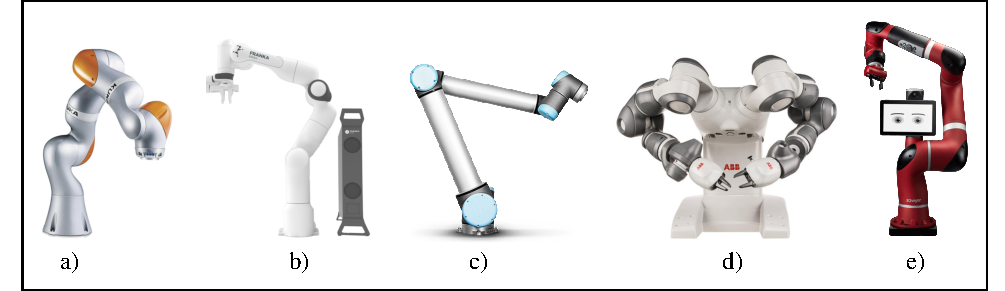
\includegraphics[width=1\linewidth]{\figurepath/robots}
\caption{(a) KUKA LBR iiwa, (b) Franka Emika arm, (c) Universal Robots UR10, (d) ABB YuMi and (e) Rethink Robotics Sawyer.}
\label{fig:robots}
\end{figure} 
%The Barrett arm
%The Mitsubishi PA10
The KUKA LBR iiwa \cite{iiwa-url} is a fully torque controlled robot designed as a continuation of the DLR lightweight robotic arms lineup. Based on the DLR LWR-III, it has 7 degrees of freedom, weighs $14~kg$ and is able to achieve a unitary payload-to-weight ratio. In addition to its torque sensors at each joint, the robot is equipped with redundant joint position sensors on both actuation and link sides. \\
%
Franka Emika \cite{Franka-url} is a highly cost competitive robotic arm also aimed for human-robot collaboration. Launched in 2017, despite its low cost, it has similar features to other more expensive systems. The robot is equipped with torque sensors in all its 7 joints and can handle payloads up to $3~kg$. \\
%
UR10 from UNIVERSAL ROBOTS \cite{UR10-url} is a commercially available lightweight redundant arm with a payload of $10~kg$. With only 6 degrees of freedom, it has however a great working range with joints that can perform  complete $+/-360~°$ rotations. \\
%
ABB Yumi is a collaborative dual-arm robot with 14 axes of freedom (7 in each arm) \cite{YuMi-url}. It includes flexible hands, parts feeding systems and embedded cameras. With a payload of $0.5~kg$, this robot is specifically designed for small parts assembly. \\
%
Sawyer is the latest robot model from Rethink Robotics. Based on the two armed Baxter, with 7 degrees of freedom, it exhibits better accuracy and repeatability performances \cite{Sawyer-url}. With embedded vision, the robot is able to handle loads up to $4~kg$ and thanks to its torque sensors, it can also be fully torque controlled. 

While other robot providers have recently started to propose collaborative versions of their standard robots, the five examples cited hereby remain forerunners of this domain.
%The system has a LED tablet as a face that can be used to render its interaction with humans more effective and intuitive.
%
%This is the case of robot manipulators actuated
%through pulleys and steel cables, where the elasticity is deter-
%mined by the elastic coefficient of the cables. Cable actuation can
%ensure human-like dimensions of the artifact, lightness and also
%anthropomorphic mass distributio
%%%%%%%%%%%%%%%%%%%%%%%%%%%%%%%%%%%%%%%%%%%%%%%%%
\section{Control}
%1)Parler des difrrentes techniques utuliser pour les controleurs d'interaction : ex force/position. 
%2)Parler du plus importaht qui est le impedance controller.
%3)Dire que sa formulation standart est por les robots stiff. 
%4)ensuite dire les problems que ça pose pour les robots élastiques. 
%5)Dires les nouvelles formulations.
%6) Parler des autres stratégie comme celle de sami. 
%
%
%The idea of extending human-like impedance control to robots aimed for physical interaction stared with the pioneering work of Hogan \cite{part1985impedance} The basic objective of such controllers is the achievement of a desired dynamical relation between external forces applied to the robot and its resulting movement. In many robotic  applications this dynamical behaviour is usually specified in terms  of stiffness and damping matrices with respect to some Cartesian  coordinates
%
%Which has since been extended to intrinsically flexible joint robots in [79, 16, 309, 15, 2015]
%
%
%A Passivity  Based Cartesian  Impedance  Controller for Flexible Joint Robots 
%- Part I: 
%/However in many robotic  applications this dynamical behaviour is specified in terms  of stiffness and damping matrices with respect to some Cartesian  coordinates 
%/A straight forward application of these techniques to a flexible joint robot  therefore usually will not  lead to a satisfactory performance'. In this paper an  impedance  control law is proposed  which 
%is designed for flexible joint robots. The desired  impedance is assumed to be  a  second  order  mass- spring-damper  system.  Furthermore only  the achievement of stiffness and  damping is  considered herein,  while  the inertial behaviour is left unchanged. 
%/However it has been shown that in practice only quite unsatisfactory results can be achieved with a restriction to purely motor position  (and velocity) based feedback controllers (without additional  non collocated  feedback) for the case of a  flexible joint robot. In some  works a controller structure based on a feedback of the joint torques as well as the link side positions was  considered and it  was  shown that this can lead to better results (see e.g. [IO]). This has  also  already been  verified experimentally with  the  DLR-light-weight-robots [2]
%
%
%
%A tank-based approach to impedance control with variable stiffness.
%The impedance control provides a compliant behaviour during the interaction and regulates the dynamic response of the robot end-effector to interaction forces by establishing a suitable virtual mass-spring-damper system on the end-effector
%Excessive contact force between the manipulator and the
%environment should be prevented. Since humans control the force exerted on an object by adapting their arm stiffness, in a similar way the robot should be able to change the stiffness of its arm while performing an interaction task. The
%/In order to imitate the surgeon’s behaviour, an impedance control with variable target stiffness is proposed in this paper
%/The contribution of this paper is a modified impedance
%control strategy that allows to reproduce a variable stiffness while preserving the passivity, and therefore a stable behaviour both in free motion and in interaction with partially known environments, of the robot.
%//Analogously to the stiffness of a human arm that is adapted for different tasks; [] propose a control strategy that allows to reproduce a variable stiffness while preserving the passivity and therefore a stable behaviour of the robot, both in free motion and during physical interaction.
%
%
%An  ISO10218-compliant  adaptive  damping  controller
%for  safe  Physical  Human-Robot  Interaction:
%the  International  Organization  for
%Standardization  included  requirements  for  a  safe  industrial
%robot.  This  standard  specifies  that  any  robot  must  respect
%velocity,  power  and  contact  force  limits  at  the  tool  control
%point (TCP) in the presence of a human
%//An  alternative  comes  from  control,  typically  impedance
%control [10], and its modified versions for force tracking [11],
%force  limitation  [12],  adaptive  damping  [13]  or  exploiting
%redundancy  [14].  However,  to  the  best  of  our  knowledge,
%the only work that explicitly tackles the ISO1028-2011 from a control viewpoint is [15].
%//In  this  paper,  we  propose  an  adaptive damping  controller  that  fulfills  the  ISO10218  requirements  by limiting  the  tool  velocity,  power  and  contact  force  online  (and only  when  needed
%//
%Adaptive Human–Robot Interaction Control for
%Robots Driven by Series Elastic Actuators:
%For the
%robot driven by SEAs, which closely interacts with humans, the
%interaction force between the human and the robot should be
%considered as an important safety measure, and it is necessary
%to control not only the position but also the interaction force. To
%realize the interaction control task, hybrid position/force con-
%trol [19] and impedance/admittance control [20]–[25] have been
%proposed for different robots.\\
For robots that physically interact with humans, the interaction force should imperatively be considered as an important safety quantifier \cite{ISO15066PDF}. It is thus necessary to control not only the position but also the interaction force \cite{ikuta2001safety}. To design an interaction oriented controller, the idea of force control has been an active research topic with initial work in \cite{whitney1977force} and \cite{mason1981compliance}. It can be divided into two main approaches \cite[Chapter~9]{siciliano2016springer}: 
\begin{itemize}
\item direct force control that uses an explicit closure of a force feedback loop. A widely adopted strategy from this category is hybrid force/position control that allows the user to simultaneously specify a desired motion along the unconstrained task directions and a desired contact force/moment along the constrained task directions \cite{raibert1981hybrid}, \cite{khatib1987unified}. A major concern with this approach is that for good performances, an accurate model of the contact properties of the environment of the robot is needed.
\item Indirect force control without explicit closure of a force feedback loop. Force control in this case is achieved via motion control. The most widely used scheme from this category is probably impedance control. The idea of extending human-like impedance control to robots aimed for physical interaction stared with the pioneering work of Hogan \cite{hogan1984impedance}. The basic objective of such controllers is the achievement of a desired dynamical relation between external forces applied to the robot and its resulting movement. In many robotic  applications this dynamical behaviour is specified in terms  of equivalent mass, stiffness and damping matrices with respect to some Cartesian coordinates \cite{ott2010unified}:
%\begin{equation}
%F_{ext} = M^*(\ddot{x}-\ddot{x}^*)+D^*(\dot{x}-\dot{x}^*)+K^*(x-x^*),
%\label{eq:impedance_cntrl}
%\end{equation}
%where $x$, $x^*$ $\in \mathbb{R}^{6}$ are the current and desired pose for the robot's end-effector, $F_{ext} \in \mathbb{R}^{6}$ is the external wrench (see Fig.~\ref{fig:damping_cntrl}) and $M^*, K^*, D^* \in \mathbb{R}^{6X6}$ are the desired Cartesian inertia, stiffness and damping matrices. 
\begin{equation}
F_{ext} = M^* \vect{\ddot{e}}+D^*\vect{\dot{e}}+K^*\vect{e},
\label{eq:impedance_cntrl}
\end{equation}
The terms $\vect{e}$, $\vect{\dot{e}}$ and $\vect{\ddot{e}}$ are not explicitly defined here because they are representation dependent (see \cite{Siciliano2008}). They respectively correspond to the position and orientation errors of the end-effector of the robot with respect to a desired pose $x^*$ and their first and second derivatives. $F_{ext} \in \mathbb{R}^{6}$ is the external wrench (see Fig.~\ref{fig:damping_cntrl}). $M^*, K^*, D^* \in \mathbb{R}^{6X6}$ are the desired Cartesian inertia, stiffness and damping matrices. 
\vspace*{-5mm}
\begin{figure}[H]
\captionsetup{width=.86\linewidth}
\centering
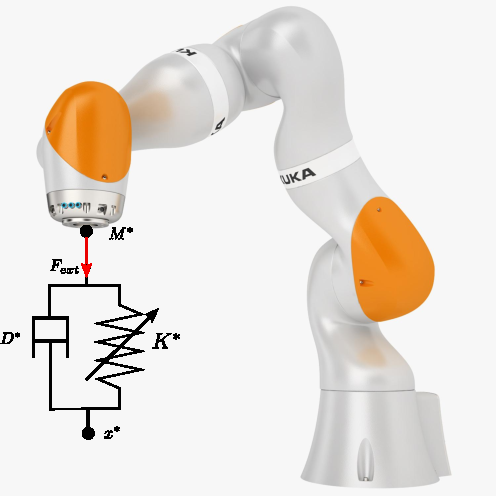
\includegraphics[width=0.35\linewidth]{\figurepath/damping_cntrl}
\caption{Desired mechanical behaviour expressed by a mass-spring-damper like system.}
\label{fig:damping_cntrl}
\end{figure} \\
\vspace*{-2mm}
Impedance control laws  provide accurate trajectory tracking in free motion while displaying passive properties (mass-spring-damper like system) in response to unexpected collisions. To overcome position tracking accuracy and stability problems when implementing impedance control for flexible joint robots, adapted schemes that take into account the robot's joints elasticity have been proposed \allowbreak\cite{zollo2005compliance}, \cite{albu2007unified}, \cite{ott2008passivity}, \cite{ott2008cartesian}.   
\end{itemize}
%Control algorithms designed for robots with non compliant actuators can
%guarantee a stable behaviour even if a certain degree of elasticity is present in the actuation system or in the structure of the robot. The drawback, however, is a typical degradation of performances in terms positioning accuracy in tracking tasks for the robot's end-effector. It may also become a source of instability in case of interaction between the robot and the environment, as undesirable effects of chattering during contact can appear.
Two interesting implementations are the schemes proposed by Schindlbeck et al. and Ficuciello et al. In \cite{schindlbeck2015unified}, a novel Cartesian passivity-based controller that combines both force tracking and impedance control is presented. To ensure the stability of the controller and its robustness with respect to contact loss, the concept of Task-energy tanks is used \cite{ferraguti2013tank}. Basically, the \textit{energy tank} dynamically cancels out the non-passive terms which arise during contact such that the overall system with its combined force/impedance controller is passive. In \cite{ficuciello2015variable}, a Cartesian impedance controller which parameters are modulated to enhance the comfort perceived by humans during physical interaction is presented. Better performances in terms of compromise between accuracy and execution time are obtained.  \\
%Apart from direct and indirect contact force control
Apart from the cited strategies, various other control  approaches using internal and external force/torque sensors have been developed to handle safety for human-robot interaction during pre and post impact/contact phases \cite{ebert2002safe}, \cite{lumelsky1993real}, \cite{ikuta2003safety}. Haddadin in \cite{haddadin2008collision} and De Luca in \cite{de2006collision} present different strategies to reduce the effect of undesired impacts. A collision detection parameter based on the estimated external torque is introduced and used with joint torque feedback to scale down the link inertia obtaining a ``lighter" robot that ``flees" from the collision area. An other strategy is to use the disturbance input (sensed external torque) to slow the robot until zero velocity is reached then pushing it back along its original path.  Heizmann and Zelinsky in \cite{heinzmann2003quantitative} propose a safety criterion based on the \textit{potential impact force} to filter the control torque of the system. The introduced controller allows one to  consider two potential contact points at the same time for a real-time implementation.
As the degree of potential injury is directly related to the mass and velocity of the colliding objects, the controller proposed in \cite{haddadin2012truly} takes into account the reflected robot inertia along a collision direction to decide about the maximum operational point velocity. The bounds on this velocity are based on experimental results relating mass, velocity, geometry and medically observable soft tissue injury by systematic drop-testing experiments with pig abdominal wall sample.
By making use of the redundancy property of a KUKA/DLR lightweight arm, \cite{de2008exploiting} proposes a physical interaction strategy that is able to react safely to collisions while continuing to execute as much possible of the original task. Finally, if physical interaction between the robot and its environment is prohibited, obstacle avoidance techniques such as presented in \cite{flacco2012depth} and \cite{de2012integrated} can be used. Considering the limited dynamic capabilities of robots, these techniques to avoid physical contact can however fail in case of highly dynamic environments.
%
%
%%Variable Impedance Control of Redundant Manipulators for Intuitive Human–Robot Physical Interaction
%The main idea of the paper is that of using in a synergic
%way the robot’s redundancy and the modulation of the Carte- sian impedance parameters to enhance the performance during human–robot physical interaction.
%/On the other hand, the variable impedance with a suitable modulation strategy for parameters’ tuning outperforms the constant impedance, in the sense that it enhances the comfort perceived by humans during manual guidance and allows reaching a favorable compromise between accuracy and execution time.
%Index
%
%
%
%
%
%
%In fact, elasticity of
%mechanical transmissions induces position errors at the robot’s
%end effector because of static deformation under gravity. In addi-
%tion, it may generate lightly damped vibrational modes, which
%reduce robot accuracy in tracking tasks
%. Yet, it may become a source of instability in case of interaction between the robot and the environment, possibly leading to undesirable effects of
%chattering during contact
%
%
%
%
%%Unified Passivity-Based Cartesian Force/Impedance Control for Rigid and Flexible Joint Robots via Task-Energy Tanks
%//In this paper, we strive for a robust passivity-based ap-
%proach by combining force tracking with impedance con- trol based on the concept of energy tanks
%//we present a solution that is able to get rid of the inherent drawback of force and set-point based indirect force control: the low robustness with respect to contact loss and the according possibility of unsafe abrupt robot motions.
%//Contact-non-contact stabilization
%//In this paper we proposed a novel Cartesian passivity-
%based force/impedance controller. In order to be able to systematically fuse both concepts, we applied the concept of energy tanks such that the force tracking controller, impedance controller, energy tank, and motor dynamics together yield a passive system. Furthermore, our approach is able to cope with contact discontinuities such that no unwanted rapid motions due to contact loss may occur
%
%
%%Springer robotics handbook

%Active interaction control strategies can be grouped into
%two categories: those performing indirect force control
%and those performing direct force control. The main dif-
%ference between the two categories is that the former
%achieve force control via motion control, without ex-
%plicit closure of a force feedback loop; the latter instead
%offer the possibility of controlling the contact force and
%moment to a desired value, thanks to the closure of
%a force feedback loop.
%To the first category belongs impedance control (or
%admittance control) [9.7, 8], where the deviation of the
%end-effector motion from the desired motion due to the
%interaction with the environment is related to the con-
%tact force through a mechanical impedance/admittance
%with adjustable parameters. A robot manipulator under
%impedance (or admittance) control is described by an
%equivalent mass–spring–damper system with adjustable
%parameters. This relationship is an impedance if the
%robot control reacts to the motion deviation by gener-
%ating forces, while it corresponds to an admittance if
%the robot control reacts to interaction forces by impos-
%ing a deviation from the desired motion. Special cases
%of impedance and admittance control are stiffness con-
%trol and compliance control [9.9], respectively, where
%only the static relationship between the end-effector po-
%sition and orientation deviation from the desired motion
%and the contact force and moment is considered. Notice
%that, in the robot control literature, the terms impedance
%control and admittance control are often used to refer to
%the same control scheme; the same happens for stiffness
%and compliance control. Moreover, if only the relation-
%ship between the contact force and moment and the end-
%effector linear and angular velocity is of interest, the
%corresponding control scheme is referred to as damping
%control [9.10].
%Indirect force control schemes do not require, in
%principle, measurements of contact forces and mo-
%ments; the resulting impedance or admittance is typi-
%cally nonlinear and coupled. However, if a force/torque
%sensor is available, then force measurements can be
%used in the control scheme to achieve a linear and de-
%coupled behavior.
%
%
%Differently from indirect force control, direct force
%control requires an explicit model of the interaction
%task. In fact, the user has to specify the desired motion
%and the desired contact force and moment in a con-
%sistent way with respect to the constraints imposed
%by the environment. A widely adopted strategy be-
%longing to this category is hybrid force/motion control,
%which aims at controlling the motion along the uncon-
%strained task directions and force (and moment) along
%the constrained task directions. The starting point is the
%observation that, for many robotic tasks, it is possible to
%introduce an orthogonal reference frame, known as the
%compliance frame [9.11] (or task frame [9.12]) which
%allows one to specify the task in terms of natural and
%artificial constrains acting along and about the three
%orthogonal axes of this frame. Based on this decompo-
%sition, hybrid force/motion control allows simultaneous
%control of both the contact force and the end-effector
%motion in two mutually independent subspaces. Simple
%selection matrices acting on both the desired and feed-
%back quantities serve this purpose for planar contact
%surfaces [9.13], whereas suitable projection matrices
%must be used for general contact tasks, which can also
%be derived from the explicit constraint equations [9.14–
%16]. Several implementation of hybrid motion control
%schemes are available, e.g., based on inverse dynam-
%ics control in the operational space [9.17], passivity-
%based control [9.18], or outer force control loops closed
%around inner motion loops, typically available in indus-
%trial robots [9.2].
%
%
%
%
%
%
%
%
%%Compliance Control for an
%%Anthropomorphic Robot with
%%Elastic Joints: Theory and
%%Experiments
%Control algorithms conceived for completely rigid robots may
%guarantee a stable behaviour even if a certain degree of elasticity in
%the actuation system and motor transmission elements, or in the
%link structure, is present. The price to pay, however, is a
%typical degradation of robot performance. In fact, elasticity of
%mechanical transmissions induces position errors at the robot’s
%end effector because of static deformation under gravity. In addi-
%tion, it may generate lightly damped vibrational modes, which
%reduce robot accuracy in tracking tasks
%. Yet, it may become a source of instability in case of interaction between the robot and the environment, possibly leading to undesirable effects of
%chattering during contact
%
%Several solutions have been proposed in the literature to cope
%with the control issue of robot manipulators with rigid joints in-
%teracting with the working environment. They range from the con-
%cept of active compliance to the concept of making the robot’s end
%effector to behave as a mechanical impedance see, e.g., Ref.9for a survey , up to the hybrid position/force control approach 10
%
%This paper is aimed at presenting a complete theoretical formu-
%lation of a compliance control in the Cartesian space plus gravity
%compensation for robots with elastic joints. The controller consists
%of a proportional-derivative action plus gravity compensation, as
%for rigid robots, but a new position variable, named the gravity-
%biased motor position, is introduced 18. This allows using only
%the position and velocity information, available from the position
%sensors on the rotors, to achieve an easy regulation of compliance
%in the Cartesian space. Asymptotic stability is proven for two Formulations of the control law, namely, compliance control with constant gravity compensation as in 15, and compliance control with on-line gravity compensation.
%  
%  
%  
%% On the Passivity-Based Impedance Control of Flexible Joint Robots
%In this paper, an impedance control law is proposed that is designed for flexible joint robots. The desired impedance is as- sumed to be a mass–spring–damper system. Furthermore, only the achievement of stiffness and damping is considered herein, while the inertial behaviour is left unchanged. In case of a robot with rigid joints, such a stiffness and damping behaviour could, in principle, be implemented quite easily with a PD-like con- troller (formulated in the relevant coordinates). In [10], it was proven that a motor-position-based PD-controller leads to a sta- ble closed-loop system also in case of a robot with flexible joints. Furthermore, in [11], a stability analysis of a hybrid position/force controller for a flexible joint robot without grav- itational effects was presented. However, it has been shown that, in practice, often only quite limited performance can be achieved with a restriction to purely motor position (and ve- locity) based feedback controllers (without additional noncol- located feedback) for the case of a flexible joint robot. In some works, a controller structure based on a feedback of the joint torques as well as the link side positions was considered, and it was shown that this leads to an increase of performance (see, e.g., [12]). This has also already been verified experimentally with the DLR lightweight robots [13]  

%\section{Quantifying human safety}
%a systematic method for tuning the passive elasticity of the individual joints is still missing. This tuning is typically performed using experimental trial and error processes and very little information on the criteria and methodologies used is available. This work studies the effects of passive compliance on the key parameters of the robotic systems including natural frequency, damping ratio, Cartesian
%
%  
%  
%is 
%traditional to 
%make 
%the 
%interface 
%between 
%an 
%actuator 
%and its load 
%as 
%stiff 
%as possible. Despite this tradition, reducing 
%interface  stiffness  offers 
%a  number 
%of 
%advantages,  including 
%greater shock  tolerance,  lower  reflected 
%inertia, 
%more 
%accurate 
%and 
%stable 
%force control, less inadvertant damage to 
%the environ- 
%ment, and 
%the 
%capacity 
%for 
%energy 
%storage. 
%As 
%a trade-off, reduc- 
%ing 
%interface    stiffness   also    lowers    zero    motion 
%force 
%bandwidth
%
%
%
%%Why we use intrinsically flexible joints
%
%
%
%for an improved
%torque/mass ratio and energy efficiency with new con-
%trol methods to exploit the stiffness and damping prop-
%erties are required
%
%
%
%By considering the phys-
%ical contact of the human and the robot in the design
%phase, possible injuries due to unintentional contacts
%can be considerably mitigated
%
%%%%%%
%%%%%%
%%%%%%
%In order for humans and robots to interact in an effective and intuitive manner, robots must obtain information about the human affective state in response to the robot's actions. This secondary mode of interactive communication is hypothesized to permit a more natural collaboration, similar to the "body language" interaction between two cooperating humans. This paper describes the implementation and validation of a hidden Markov model (HMM) for estimating human affective state in real time, using robot motions as the stimulus. Inputs to the system are physiological signals such as heart rate, perspiration rate, and facial muscle contraction. Affective state was estimated using a two- dimensional valence-arousal representation. A robot manipulator was used to generate motions expected during human-robot interaction, and human subjects were asked to report their response to these motions. The human physiological response was also measured. Robot motions were generated using both a nominal potential field planner and a recently reported safe motion planner that minimizes the potential collision forces along the path. The robot motions were tested with 36 subjects. This data was used to train and validate the HMM model. The results of the HMM affective estimation are also compared to a previously implemented fuzzy inference engine.
%
%
%Providing a robot with the capability of predicting a person's behaviour by estimating his affective state can considerably improve the quality of the human-robot interaction. Input data like verbal or non verbal signals (e.g. facial expressions of the person) can be used as input data to adapt the behaviour of the robot Indeed, for a person, interaction with such a robot can be more effective and intuitive. 
%
%
%
%Such application cases and related technical issues raise crit-
%ical questions of physical safety, reliability, and, more general-
%ly, communication and operating robustness. All these aspects
%can be captured by the concept of dependability
%
%
%gestures, gait, facial expressions, dialogue, online learning
%
%The new KUKA LWR design can be considered as intrinsically safe and therefore suitable for human-robot-physical interaction
%
%It should be safeguarded as a “traditional”
%robot system (people are separated from it)
%\\
%\\
%%%%%%%%%%%%%%%%%%%%%%%%%%%%%%%%%%%%%%%%%%%%%%%%%µµµµµµµµµµ
\section[Safety standards]{Safety standards for human-robot interaction}
%% Safety standards for human-robot interaction
The original safety standard for traditional industrial robots is the ISO 10218 initially edited in 1992. During its last revision, the decision was taken to separate it into two parts: ISO 10218-1 and ISO 10218-2 lately revised in 2011 \cite{fryman2014updating}. On the one hand,  ISO 10218-1 \cite{ISO10218PDF1} is particularly dedicated to manufacturers; It describes dangerous phenomena related to robots and gives recommendations and guidelines for protective measures and safe design indications in line with the machinery directive 2006/42/EC. 
Technical specifications in this part concern, in a non-exhaustive way, definitions and requirements related to: singularity, protection against hazards that can be caused by mechanical transmission, requisites in case of loss of power, performances of safety control circuits, conditions relative to control modes and limitations of power and strength plus the description of emergency stop functions.
On the other hand, ISO 10218-2 is drafted to give more diverse safety requirements and guidance to integrators for the installation of industrial robots and industrial robot systems ``robot+cell(s)". ISO 10218-2 \cite{ISO10218PDF2} describes how to properly conduct a task-based risk assessment to eliminate or reduce risks associated with hazards to personnel: hazards engendered by the design, implementation and use of these systems. The newest and most exciting utility introduced in ISO 10218-1 and -2 is the direct interaction between robotic systems and human-operators. Indeed, historically, for safety reasons, industrial robots are usually separated from humans by the mean of physical segregation, i.e., cages. ISO 10218-1 and -2 give general guidelines regarding safety requirements for human-robot interaction but do not provide the needed metrics for the design of collaborative robots, tasks and control strategies. In these standards, four collaborative techniques are considered:
\begin{itemize}
\item Safety-rated monitored stop: the system does a monitored stop so the human can enter its workspace to perform an assigned task. The robot system resumes its autonomous task once the operator is out.
\item Hand-guiding: based on a safety-rated monitored stop, a human-operator can take control of the end-effector to move the robot. Once motion is complete, a monitored stop is issued again as the person exists the workspace.
\item Speed separation monitoring: the robot arm and the human maintain a safe distance from each other. Depending on this distance, the speed of the robot is reduced.
\item Power and force limiting: Power and force of the robot are limited by design or control during physical interaction.
\end{itemize}
The latest document from the International Standardization Organization (ISO) fully dedicated to human-robot collaboration is the ISO/TS 15066 \cite{ISO15066PDF}. Issued in 2016, this Technical Specification (TS) is a game changer for the robotics industry as it gives specific and detailed metric-based safety guidance needed to assess and control risks during human-robot interaction. Pressure, force and even transferred energy limit values based on injury and pain sensitivity thresholds for various areas of the human body are provided. It states for example the following limits for allowing human-robot interaction at the hands level: maximum transferred energy $E=0.49~J$ and maximum permissible force $F=140~N$. 
%%%%%%%%%%%%%%%%%%%%%%%%%%%%%%%%%%%%%%%%%%%%%%%%%
\section{Discussion and proposed contributions}
%\subsection{Safety as constraint}\\
\subsection{Considerations when dealing with safety during human-robot interaction}
Although the presented state-of-the-art gives various propositions on how to handle safety during human-robot interaction, there are still numerous issues to be addressed, specifically in terms of satisfying the safety limit values recommended by the recent ISO/TS 15066 standard \cite{ISO15066PDF} and the discontinuity problems that may occur when switching between control modes for different interaction phases, e.g., at collisions and at contact establishment and release. In this sense, the work presented in this thesis aims at closing the gap and defining a generic framework to control a robotic arm during different interaction phases with a human-operator. Safety in the controller is therefore included as a constraint.\\
The following aspects are considered for the formulation of safety constraints and a safe human-robot interaction controller: 
\begin{itemize}
\item Safety indicators $I$ related to the safety limit values provided in ISO/TS 15066 \cite{ISO15066PDF} that can be expressed at any point of a multi-body robot must be formulated. These indicators should reflect the amount of danger the robot exhibits towards a nearby human-operator during different interaction phases: as the human enters the workspace of the robot, after the establishment of a deliberate or non-deliberate physical contact and as contact is released.
%Therefore, these two parameters are not suitable for our purpose.   
\item The formulation of safety criteria $I_{limit}$ that represent the maximum values allowed for the safety indicators and that consequently bound the dynamics of the robot for each interaction phase. These safety criteria should also be based on the safety metrics given by the ISO/TS 15066 standard \cite{ISO15066PDF}.
\item  Finally using the safety indicators and safety criteria, the formulation of safety constraints that depend on the joint control input $\tau$:  $I(\tau) \leq I_{limit}$. These constraints can then easily be included in an optimization control scheme.
\end{itemize}
The different safety indicators from the literature are usually only useful during one interaction phase. Velocity of the end-effector of the robot for example is significant only during the movements of the robot and therefore cannot be used as a safety indicator during physical contact. Contact forces on the other hand can only be evaluated during physical interaction. More generic indicators should therefore be proposed. \\
For a given shape of the contact surface, two parameters are source of danger during human-robot interaction: the impact force created at collision and the contact force generated after the establishment of a physical contact. The most generic way to include and consider these parameters for the formulation of  safety indicators is to use energy. Indeed, energy is a universal quantity that can describe most of the physical phenomena occurring during human-robot interaction. The impact force for example is directly related to the amount of kinetic energy dissipated at collision and the contact forces mostly derive from the amount of \textit{potential energy} that accumulates in controller of the robot during physical contact. Velocity, inertia and also the resulting position error during physical contact are all part of the mathematical expression of energy. 
%It is therefore used in Chapter~\ref{chap:safety} and Chapter~\ref{chap:safety2} as a safety indicator to be monitored and modulated to insure the safety of a person physically interacting with a robotic arm.     
Safety during human-robot interaction can therefore be ensured by modulating the amount of energy instantaneously deployed by the robot. The main contributions presented in \textbf{Chapter~\ref{chap:safety}} regarding safety during human-robot interaction are as follows:
\begin{itemize}
\item the formulation of kinetic and \textit{potential energy}\footnote{The term ``\textit{potential energy}'' here refers to the amount of energy loaded in the controller of the robot during both \textit{free} movement and physical contact phases.} based safety indicators that represent the degree of danger of a robotic arm at collision and during physical contact.
\item The formulation of safety criteria that bound the dynamics of the robot during different interaction phases: at the approach of a human-operator, at collision, during physical contact and finally as contact is released.
\item The expression of these indicators and criteria as inequality constraints related to the torque control input of the robot.
\item The introduction of the concept of ``task energy profile" to track the amount of energy used to accomplish a considered repetitive task in the most optimal way. This profile is then used to constrain the instantaneous amount of energy the robot is allowed to exhibit at every time-step.
The resulting controller renders the robot compliant to any deliberate or non-deliberate contact with its environment.
\end{itemize}
For the validation of the proposed algorithms, beyond theoretical contributions, simulation results conducted with a KUKA LWR4 serial robot that physically interacts with its environment are also presented in \textbf{Chapter~\ref{chap:safety}}. \textbf{Chapter~\ref{chap:safety2}} on the other hand presents the results of experimental applications on a real KUKA LWR4 whose energy is modulated as a human-operator enters its workspace, physically interacts with it, release contact then safely leave the workspace. In this scenario, the amount of kinetic energy deployed by the KUKA LWR4 during the approach of the human is modulated according to the operator-robot real-time distance. This distance is computed with an algorithm that uses point clouds acquired from the scene using a set of depth sensors (Kinects).





%Regarding the second point, for a given shape of the robot, two main parameters are usually considered for safety: the impact force generated at collision and the contact force generated after the establishment of physical contact. The most generic way to consider and express these parameters is to use an energetic formulation. Indeed, energy is universal  and can describe most physical phenomena occurring during human-robot interaction. An impact force for example is directly proportional to the amount of kinetic energy dissipated at collision. The contact force on the other hand derives from the amount of potential energy generated within the human-robot system during physical contact. In our work, safety during human-robot interaction is guaranteed by modulating the amount of energy instantaneously deployed by the robot. The main contributions regarding safe human-robot interaction are as following:
%\begin{itemize}
%\item The formulation of kinetic and potential energy based safety indicators that represent the degree of danger of the robot at collision and during physical contact.
%\item The formulation of safety criteria that bounds the dynamic of the robot during different interaction phases: at the approach of the human operator, at collision, during physical contact and finally as the contact is released.
%\item The expression of these indicators and criteria as inequality constraints related to the torque control input of a robotic arm.
%\item The introduction of the concept of "task energy profile" to track the amount of energy used to accomplish a considered repetitive task in the most optimal way. This profile is used to constrain the instantaneous amount of energy the robot is allowed to exhibit at every time-step.
%The resulting controller renders the robot compliant to any deliberate or non-deliberate contact with its environment.
%\end{itemize}
%For the validation of the proposed algorithms, beyond the theoretical contributions, simulations are performed on a KUKA LWR4 serial robot that physically interacts with its environment. In Chaptre  experimental applications 

%For the validation of the proposed algorithms, beyond the theoretical contributions, simulation and experimental applications are performed on a KUKA LWR4 serial robot. 



\\
%The goal of the presented work is to seek answers for the following questions: 
%\begin{itemize}
%\item For reactive control problems, i.e., control problems where the task to be performed is not known in advance but discovered on-line, how is it possible to guarantee every time-step the existence of a solution to the control problem ? This solution should allow the robot to accomplish at best its prescribed task and at the same time to strictly comply with existing constraints, among which, constraints related to the physical limitations of its actuators and joints.
%\item How to integrate the human operator within the control loop of the robot so that physical contact can be safely engaged and de-engaged ? 
%\end{itemize} 
%Regarding the first point, our work arises as the continuity of previous results developed by Sébastien Rubrecht during his PhD thesis.
%Sébastien Rubrecht introduced the concept of constraints incompatibility that appears for example when the formulation of an articular position related constraint does not take into account the amount of deceleration producible by the joint actuator. In this case, if this constraint is activated tardively, the system may not be able to cope with its position limit considering its bounded reaction capability. In his thesis, Rubrecht solved this problem for a robot reactively controlled at the kinematic level. In our work, the problem of constraints incompatibility is extended to robots controlled at the dynamic level. New mathematical formulations for the joint position and velocity constraints are introduced considering both the deceleration and jerk capabilities of the robot actuators. When included in a QP formulation of the control problem, these new expressions guarantee the existence of a constraint compliant and optimal solution as joint position, velocity, torque/deceleration and also jerk limits are simultaneously respected at the same time and at every time-step. \\
%
%Regarding the second point, for a given shape of the robot, two main parameters are usually considered for safety: the impact force generated at collision and the contact force generated after the establishment of physical contact. The most generic way to consider and express these parameters is to use an energetic formulation. Indeed, energy is universal  and can describe most physical phenomena occurring during human-robot interaction. An impact force for example is directly proportional to the amount of kinetic energy dissipated at collision. The contact force on the other hand derives from the amount of potential energy generated within the human-robot system during physical contact. In our work, safety during human-robot interaction is guaranteed by modulating the amount of energy instantaneously deployed by the robot. The main contributions regarding safe human-robot interaction are as following:
%\begin{itemize}
%\item The formulation of kinetic and potential energy based safety indicators that represent the degree of danger of the robot at collision and during physical contact.
%\item The formulation of safety criteria that bounds the dynamic of the robot during different interaction phases: at the approach of the human operator, at collision, during physical contact and finally as the contact is released.
%\item The expression of these indicators and criteria as inequality constraints related to the torque control input of a robotic arm.
%\item The introduction of the concept of "task energy profile" to track the amount of energy used to accomplish a considered repetitive task in the most optimal way. This profile is used to constrain the instantaneous amount of energy the robot is allowed to exhibit at every time-step.
%The resulting controller renders the robot compliant to any deliberate or non-deliberate contact with its environment.
%\end{itemize}
%For the validation of the proposed algorithms, beyond the theoretical contributions, simulation and experimental applications are performed on a KUKA LWR4 serial robot. 
%%%%%%%%%%%%%%%%%%%%%%%%%%%%%%%%%%%%%%%%%%%%%%%%%
\subsection{Considerations when dealing with constraints}
The formulation of safety related constraints usually depend on sensory input that gives \textit{online} information about the dynamic environment the robot interacts with. The controller in this case \textit{reactively} cope with these constraints as it is impossible to perform a pre-planification of \textit{safe movements} for the robot without accurate data about the present and future dynamics of its environment. \\
Reactive controllers are usually formulated and solved to convert the operational inputs (user specified objectives and constraints) into joint inputs and this, at each time-step. The impact of the retained solution on the \textit{solvability} of future control problems is rarely considered and therefore, issues of \textit{constraints incompatibility} may occur. Consequently, this can render the control problem impossible to solve in the future without violating the imposed constraints. \\

To better understand the problem of \textit{constraints incompatibility}, the following scenario in which a robot interacts with its dynamic environment is considered $\ll$ a moving telemanipulated robotic arm must keep a safe distance $d_{s}$ from an obstacle $O$ entering its \allowbreak workspace $\allowbreak \gg$ (see Fig.~\ref{fig:dampdzdl})
\begin{figure}[H]
\captionsetup{width=.99\linewidth}
\centering
\includegraphics[width=1\linewidth]{\figurepath/constr_inc_scenario}
\caption{A telemanipulated robotic arm coping with a \textit{safety distance} constraint between its end-effector and an obstacle $O$ entering its workspace.}
\label{fig:dampdzdl}
\end{figure}
To prevent getting the system into a state in which its control problem cannot be solved, various specifications must be considered for the formulation of the \textit{safe distance} constraint and the reactive controller for the robot in such situation: the present and future dynamics of obstacle $O$ must be known so that the reaction of the robot can be triggered at the right time ``$t$'' considering its dynamic capabilities  in Cartesian space, i.e., producible deceleration and jerk. These reaction capabilities for a multi-body robot are configuration dependent and are function of the deceleration and jerk capabilities of its actuators in joint space. Moreover, minimum values for these dynamic capabilities in operational space cannot be guaranteed without knowing the future configurations of the robot. \\
These exposed considerations make the control of the robot in such scenario a complex problem to solve. However, if the present and future dynamics of both the robotic arm and obstacle $O$ are predictable, a \textbf{formal optimal} solution can be computed as follows: considering the dynamics of obstacle $O$ and minimum guaranteed deceleration and jerk capabilities of the end-effector of the robot in Cartesian space, the optimal time ``$t$'' at which the robot must start \textbf{braking} using its \textbf{maximum producible deceleration and jerk} so it can stop exactly when the distance between its end-effector and the moving obstacle $O$ is equal to $d_{s}$, can be computed. The robot can then keep this distance by moving in the opposite direction as it is chased by obstacle $O$. \ul{Note that in this scenario, if the reaction of the robot is triggered after the optimally computed instant ``$t$'', the robot will never be able to cope with the \textit{safe distance} constraint considering its limited reaction capabilities}. A \textit{constraints incompatibility} problem between the \textit{safe distance} constraint and the bounded maximum producible deceleration and/or jerk will inevitably occur as it becomes impossible to cope with both constraints at the same time during the movement of the robot. 

%In addition to these various challenges that are summarized in Fraichard's safety criteria\footnote{\begin{itemize}\item To decide its future motion, a robotic system should consider its own dynamics; \item To decide its future motion, a robotic system should consider the future behavior
%of the environment; \item To decide its future motion, a robotic system should reason over an infinite time-horizon.\end{itemize}} \cite{fraichard2007short}, the robot's controller in the proposed scenario must take into account the very own actuation limitations of its actuators, i.e. joint rate and articular position limits. From a closer point of view, articular constraints related to these physical limitations are actually a simplified version of the \textit{safe distance} constraint. Analogously, the moving obstacle in Fig.~\ref{fig:dampdzdl} relate to the static joint rate and position limits, the moving end-effector correspond to the actual position and velocity of the joints that increase towards their respective boundaries and, the deceleration and jerk capabilities in Cartesian space equate to the robot's dynamical capabilities in joint space. We recall that in this scenario, the robot is teleoperated and thus trajectories for its joints cannot be pre-planned. Articular constraints are then also handled reactively by the controller of the robot. In Chapter~\ref{chap:Constrcomp}, new formulations for the articular constraints are proposed. These new formulations take into account the robot's dynamical actuation capabilities and when included in the controller trigger the needed reaction on joint level at the right time to cope with the different articular physical limits. A solution to the control problem can be instantaneously computed and the viability of the state of the robot can be guaranteed for all its future movements.  
In addition to these various challenges related to the \textit{safe distance} constraint, the controller of the robot in the proposed scenario must also take into account the very own actuation limitations of the system's actuators, i.e., the articular velocity and position limits in addition to the constraints on the max/min producible articular acceleration and jerk. From a closer point of view, the articular constraints related to these physical limitations are actually a \textit{simplified} version of the \textit{safe distance} constraint. Analogously, the instantaneous distance to the moving obstacle in Fig.~\ref{fig:dampdzdl} relates to the static articular velocity and position limits, the position of the moving end-effector corresponds to the actual position or velocity of the constrained joints that increase towards their respective boundaries; and the deceleration and jerk capabilities in Cartesian space equate to the dynamical capabilities of the robot in joint space. We recall that in this scenario, the robot is reactively controlled and trajectories for its joints cannot be pre-planned. Consequently, the constraints related to its articular velocity and position boundaries are also handled reactively by the controller. To avoid \textit{constraints incompatibility} problems regarding these two constraints,  their classic formulations usually used in the literature are modified in \textbf{Chapter~\ref{chap:Constrcomp}} to include the dynamic capabilities of the robot in joint space, namely, the maximum producible articular deceleration and jerk:
\begin{itemize}
\item the formulation of the constraint on articular velocity is modified to include the maximum producible articular jerk used to bring the joint's acceleration to $0$ at the activation of the constraint and;
\item the formulation of the constraint on articular position is modified to include the maximum producible articular deceleration and jerk used to bring both the articular acceleration and velocity to $0$ at the activation of the constraint.  
\end{itemize}
The problem of \textit{constraints incompatibility} relates to the notion of \textit{safety at the control level} about which, Fraichard in 2007 proposed 3 main criteria \cite{fraichard2007short}:
\begin{itemize}
\item to decide its future motion, a robotic system should consider its own dynamics; 
\item to decide its future motion, a robotic system should consider the future behaviour of its environment; 
\item to decide its future motion, a robotic system should reason over an infinite time-horizon.
\end{itemize}
In his work, Fraichard assesses different control approaches for single body mobile robots regarding the definition of safety he proposed. Based on these criteria, our work in \textbf{Chapter~\ref{chap:Constrcomp}} arises as the continuity of previous results developed by S{\'e}bastien Rubrecht \cite{rubrecht2010constraints}. In his PhD thesis \cite{rubrecht:tel-00654514}, Rubrecht introduced the concept of \textit{constraints incompatibility} for  the constraints related to the articular limitations of a robotic manipulator. This problem appears for example when the formulation of a constraint on articular position does not take into account the amount of deceleration producible by the actuators of the robot. In such case, if this constraint is activated \textbf{tardively}, no sufficient time may be available for the actuator of the joint to stop its motion before exceeding the allowed position limit. In his work, Rubrecht solved this problem for a serial robot reactively controlled at the kinematic-level. Our work presented in \textbf{Chapter~\ref{chap:Constrcomp}} on the other hand, tackles the problem of \textit{constraints incompatibility} for robotic manipulators controlled at the dynamic-level (torque control) and an optimal solution to this problem regarding the articular velocity and position constraints is proposed.\\
For each of these two constraints, the new proposed formulation is derived as follows:
\begin{itemize}
\item For the constraint on articular velocity, first, the joint's discrete state during the \textit{braking phase} implicitly induced by the actuator of the join to bring its acceleration to $0$ when coping with an articular velocity limit is described. Second, the \textit{general form} of this state is derived and used to formulate the new expression of the constraint. Finally, the number $n$ of time-steps, that corresponds to the duration of the induced \textit{braking phase}, needed to optimally cope with the articular velocity limit is computed. \textbf{The constraint on the articular velocity and the one on the articular jerk are made compatible}.
\item For the joint position constraint, first, the joint's discrete state during the \textit{braking phase} implicitly induced by the actuator of the joint to completely stop its motion when coping with an articular position limit is described. Second, the \textit{general form} of this state is derived and used to formulate the new expression of the constraint. Finally, the number $n$ of time-steps, that corresponds to the duration of the induced \textit{braking phase}, needed to optimally cope with the joint position constraint is computed. \textbf{The articular position constraint together with the constraints on articular deceleration and jerk are made compatible}.
\end{itemize}
When included in a QP formulation of the control problem, the introduced new formulations of the constraints related to the articular physical limitations of the robot guarantee the existence of a constraint compliant and optimal solution as joint position, velocity, \allowbreak torque/deceleration and also jerk limits are all simultaneously satisfied during the movement of the robot. The \textit{viability} of the state of the robot is guaranteed for every control time-step.
%%%%%%%%%%%%%%%%%%%%%%%%%%%%%%%%%%%%%%%%%%%%%%%%%
\section{Related Publications}
Some of the novel developments introduced in this work have been peer-reviewed and validated with the publications listed hereafter:
\begin{itemize}
\item Meguenani, A., Padois, V., \& Bidaud, P. (2015, September). Control of robots sharing their workspace with humans: an energetic approach to safety. In Intelligent Robots and Systems (IROS), 2015 IEEE/RSJ International Conference on (pp. 4678-4684). IEEE.
\item Meguenani, A., Padois, V., Da Silva, J., Hoarau, A., \& Bidaud, P. (2017). Energy based control for safe human-robot physical interaction. In 2016 International Symposium on Experimental Robotics (Vol. 1). Springer.
\end{itemize}
%In Chapter~\ref{chap:Constrcomp}, new formulations for the articular constraints are proposed. These new formulations take into account the robot's dynamical actuation capabilities and when included in the controller trigger the needed reaction on joint level at the right time to cope with the different articular physical limits. A solution to the control problem can be instantaneously computed and the viability of the state of the robot can be guaranteed for all its future movements.




%For reactive control problems, \textit{i.e.} control problems where the task to be performed is not known in advance but discovered on-line, how is it possible to guarantee every time-step the existence of a solution to the control problem ? This solution should allow the robot to accomplish at best its prescribed task and at the same time to strictly comply with existing constraints, among which, constraints related to the physical limitations of its actuators and joints.


















%Other than the presented energy based constraint, a safety related constraint can be for example as following <<as the robot moves, it must keep a safe distance $d$ from an obstacle $o$ entering its workspace>> (see Fig.~)
%
%
%Reactive control loops are used in most robots control architectures; they are in
%charge of converting operational inputs (user specified objectives and constraints) into
%joint inputs at each time step. Algorithms are built to satisfy constraints and objec-
%tives specified at various (potentially strict) priority levels, to handle specific cases, to
%manage transitions, etc
%
%
%
%However, all these achievements address only the resolution
%of the control problem; the solvability of the problem and the impact of the retained
%solution on the future control problems is rarely studied and constraints incompatibil-
%ity recurrently occur in robotics, which inevitably implies constraints violations, thus
%compromising safety
%
% 
%The best way to handle safety related constraints is through reactive control. Indeed, as the formulation of such constraints depend io,n     
%
%
%Other than safety related constraints
%
%These different contributions provide an initial response to the fixed goals; However, the presence of dynamic constraints (e.g. mobile obstacles) and human operators around the robot highlight other concerns that must be dealt with. The highest priority in the control of any type of human-friendly robot is to prevent of the actions of the robot from causing any harm to the human operator. 
%
%A safe human-robot collaboration requires switching between different control modes (before/after physical contact), the formulation of safety indicators to reflect the amount of danger towards the human operator, the formulation of safety criteria representing the bounds on the dynamic behaviour of the robot and finally expressing all of these as constraints related to the control parameters. 
%
%Bottom line, for a given shape, two parameters are to be considered for safety: the impact force created at the collision instant between the robot and the human operator and the contact forces generated after the establishment of physical contact. The most generic way to include and express these parameters is to use an energetic formulation. Indeed, energy is a universal entity that can describe almost all the physical phenomena occurring during human-robot interaction. For example, the impact force is directly related to the amount of kinetic energy dissipated at the collision and the contact forces derive from the amount of potential energy generated during physical contact. 
%
%Two types of constraints are considered during interaction; Static constraints where the maximum allowed limit is constant and dynamic ones where the limiting bound variates depending on other parameters (e.g. human-robot distance). For both kinds, the reaction capabilities of the robots actuators must be considered to guaranty every time step a feasible solution of the control problem. This comes down to activating the constraints on the control parameters at the right instant to ensure sufficient time to cope with the constraints. 
%



%\section{Contributions}  
%The main contributions of the presented work are as following :
%\begin{itemize} 
%\item The formulation of an energy based safety indicator that allows the modulation  of the impact force and the contact forces.
%\item The formulation of safety criteria that bound the dynamic behaviour of the robotic system considering different situations: The approach of the human operator, the establishment of physical contact and finally the releasing of contact.
%\item A theoretical study on the reformulation of two articular static constraints (position and velocity limitations) while taking into account the reaction capabilities of the robots actuators (available braking torque and jerk).
%\end{itemize} 
%For the validation of the developed algorithms, beyond the theoretical contribution, simulation and experimental application are performed on a KUKA LWR4 serial robot. For the distance acquisition, a point cloud based algorithm is used with multiple Microsoft Kinect devices. 
%. in situation of physical interaction
%Threshold limit values particularly on  Based on the "Change from pressure to pain" study conducted by the university of Mainz Institute for work in co
%
%
%
%On the other hand ISO/TS 15066 is a game changer for the industry. issued in 2016, it is fully dedicated to human-robot collaboration. This technical specification is the 
%
%lthough these standards give some initial guidelines for human-robot interaction, 
%
%ISO/TS 15066 is a game changer for the industry as it gives specific and detailed metric-based safety guidance needed to assess and control risks during human-robot interaction. Based on the "Change from pressure to pain" study conducted by the university of Mainz Institute for work in co
%
% ISO/TS 15066 provides guidelines for the design and implementation of a collaborative workspace that reduces risks to people. It specifies:
%
%    Definitions
%    Important characteristics of safety control systems
%    Factors to be considered in the design of collaborative robot systems
%    Built-in safety-related systems and their effective use
%    Guidance on implementing the following collaborative techniques: safety-rated monitored stop; hand guiding; speed and separation monitoring; power and force limiting.
%
%
%
%The technical specification includes data from a study on pain thresholds of different parts of the human body. This information can be used to develop and implement collaborative power- and force-limited robot applications.

\\
\\

%ISO 10218-2:2011 describes the basic hazards and hazardous situations identified with these systems, and provides requirements to eliminate or adequately reduce the risks associated with these hazards. ISO 10218-2:2011 also specifies requirements for the industrial robot system as part of an integrated manufacturing system
%
%
% the marking and the characteristics and principles of measure were updated for time(weather) and the distance of stop(ruling).
%
%
%
%La présente partie de l'ISO 10218 spécifie les exigences et les recommandations pour la prévention
%intrinsèque, les mesures de protection et les informations pour l'utilisation des robots industriels. Elle décrit les
%phénomènes dangereux de base associés aux robots et fournit des exigences pour éliminer ou réduire de
%manière appropriée les risques associés à ces phénomènes dangereux.
%
%
%Les exigences techniques révisées comportent, de façon non limitative, la définition et
%les exigences relatives à la singularité, la protection contre les phénomènes dangereux engendrés par la
%transmission, les exigences en cas de perte de puissance, les performances des circuits de commande de
%sécurité, l'ajout d'une fonction d'arrêt de catégorie 2, les exigences relatives à la sélection du mode et à la
%limitation de puissance et de force, le marquage et les caractéristiques et principes de mesure actualisés pour
%le temps et la distance d'arrêt.
%
%
%specifies requirements and guidelines for the inherent safe design, protective measures and information for use of industrial robots. It describes basic hazards associated with robots and provides requirements to eliminate, or adequately reduce, the risks associated with these hazards.
%
%
%fournit des recommandations pour garantir la
%sécurité lors de la conception et de la construction des robots. La sécurité dans les applications robotisées
%étant influencée par la conception et l'application de l'intégration du système de robot considéré,
%l'ISO 10218-2 donne des recommandations pour la protection du personnel pendant l'intégration, l'installation,
%les essais de fonctionnement, la programmation, l'exploitation, la maintenance et la réparation des robots.
%
%
%
%Le présent document spécifie les prescriptions de conception, les mesures de
% protection et les informations pour l’utilisation des robots afin de répondre aux
%   exigences de sécurité de la Directive «Machines» 2006/42/CE






%%Conclusion
%is  not  possible  in  general  to  ensure  safety  forever,  we  manage
%nonetheless to achieve infinite motion safety in two special cases.









	\chapter{Constraints incompatibility}
\label{chap:Constrcomp}

\setfigurepath{figures/Constrcomp}

%=========================================================================
\begin{synopsis}
%For reactive control laws, input data for the operational task are usually discovered at every time-step. In this case, constraints such as joint limits are usually handled through inequalities. Depending on how these constraints are expressed, incompatibility issues that can render the control problem unsolvable or lead to constraints violation may appear. Indeed, coping for example with an articular position or velocity limit within a small amount of time (e.g., $1~ms$) may be impossible considering the limited reaction capabilities (i.e., producible torque/deceleration and jerk) of the robot actuators. In this chapter, we study the problem of constraints incompatibility related to the articular physical limitations of a serial robot. Incompatibility cases are exposed and resolved by proposing new mathematical expressions for the articular position and velocity constraints. These new formulations take into account the available reaction capabilities of the robot actuators. Articular position constraint is reformulated to include maximum producible deceleration and jerk; And the joint rate constraint is modified to include jerk capabilities. The new formulations are implemented into a QP (quadratic programming) scheme to resolve the control problem of a redundant robot (KUKA LWR4) at the dynamic level (torque control). The resulting new expressions allow an automatic activation of the constraints, at the right time to comply with the position, velocity, torque/acceleration and jerk limits all at the same time. A solution for the optimization control problem is guaranteed every time-step, smoother control torques are produced and \textit{viability} of the state of the robot is ensured.
%For reactive control laws, input data for the operational task are usually not known a priori but discovered at every time-step. In this case, constraints such as joint limits cannot be handled beforehand through planning and are therefore included in the controller as inequalities. Depending on how these constraints are expressed, incompatibility issues (i.e., the impossibility of satisfying two or several constraints at the same time) that can render the control problem impossible to solve or lead to constraints violation may appear. Indeed, coping for example with an articular position or velocity limit within a small amount of time (e.g., $1~ms$) may be impossible considering the limited reaction capabilities (i.e., producible torque/deceleration and jerk) of a robot's actuators. In this chapter, the problem of constraints incompatibility related to the articular physical limitations of a serial robot is studied. Incompatibility cases between constraints are exposed and resolved by proposing new mathematical formulations for the joint position and velocity constraints. These new formulations take into account the dynamic capabilities of the robot's actuators. The constraints are implemented into a QP (quadratic program) scheme to solve the control problem of a redundant robot (KUKA LWR4) at the dynamic level (torque control). The resulting new expressions allow an automatic activation of the constraints, at the right time to comply with the position, velocity, torque/acceleration and jerk limits, all at the same time. A solution for the optimization control problem is available every time-step, smoother control torques are produced and the \textit{viability} of the state of the robot is guaranteed.
For reactive control laws, input data for the operational task are usually not known a priori but discovered every time-step. In this case, constraints such as joint limits cannot be handled beforehand through planning and are therefore included in the controller as inequalities. Depending on how these constraints are expressed, incompatibility issues (i.e., the impossibility of satisfying two or several constraints at the same time) that can render the control problem impossible to solve or lead to constraints violation may appear. Indeed, coping for example with an articular position or velocity limit within a small amount of time (e.g., $1~ms$) may be impossible considering the limited reaction capabilities (i.e., producible torque/deceleration and jerk) the actuators of a robot can produce. In this chapter, the problem of constraints incompatibility related to the articular physical limitations of a serial robot is studied. Incompatibility cases between constraints are exposed then resolved by proposing new mathematical formulations for the joint position and velocity constraints. The new formulations take into account the dynamic capabilities of the actuators of the robot. The constraints are implemented into a QP (quadratic program) scheme to solve the control problem of general fixed-based serial manipulators, and illustrated using a KUKA LWR4 at the dynamic control level (torque control). The resulting new expressions allow the activation of the considered constraints, at the right time to comply with the joint position, velocity, torque/acceleration and jerk limits, all at the same time. A solution for the control problem is available at every time-step, smoother control torques are produced and the ``\textit{viability}'' of the state of the robot is guaranteed over an infinite horizon of time.
%For reactive control laws, input data for the operational task are usually discovered at every time-step. In this case, constraints such as joint limits are usually handled through inequalities. Depending on how these constraints are expressed, incompatibility issues that can render the control problem unsolvable or lead to constraints violation may appear. Indeed, coping for example with an articular position or velocity limit within a small amount of time (e.g., $1~ms$) may be impossible considering the limited reaction capabilities (i.e. producible torque/deceleration and jerk) of the robot actuators. In this chapter, we study the problem of constraints incompatibility related to the articular physical limitations of a serial robot. Incompatibility cases are exposed and resolved by proposing new mathematical expressions for the articular position and velocity constraints. These new formulations take into account the available reaction capabilities of the robot. The constraints are implemented into a QP (quadratic programming) scheme to resolve the control problem of a redundant robot (KUKA LWR4) at the dynamic level (torque control). The resulting new expressions allow an automatic activation of the constraints, at the right time to comply with the position, velocity, torque/acceleration and jerk limits all at the same time. A solution for the optimization control problem is guaranteed every time-step, smoother control torques are produced and the \textit{viability} of the state of the robot is guaranteed.
%%ORIGINAL AVANT RETOUR VINCENT 
\end{synopsis}
%=========================================================================
%%%%%%%%%%%%%%%%%%%%%%%%%%%%%%%%%%%%%%%%%%%%%%%%%%%%%%%%%
                 %Introduction%
%%%%%%%%%%%%%%%%%%%%%%%%%%%%%%%%%%%%%%%%%%%%%%%%%%%%%%%%%                         
\section{Introduction}
\label{sec:intro constrcomp}
In this section, first, the general problem of \textit{constraints incompatibility} that appears when using reactive control laws is furthermore introduced and defined. The different types of constraints a robotic manipulator could face are enumerated and the various considerations regarding the \textit{constraints incompatibility problem} when coping with constraints from each type are highlighted. A brief overview of the \textit{constraints incompatibility problem} state-of-the regarding specifically the constraints related to the articular limitations of robotic manipulators is presented. Finally, the problem specifically tackled in this chapter and the contributions are summarized and the outline of the chapter is described.
%%%%%%%%%%%%%%%%%%%%%%%%%%SUBSECTION%%%%%%%%%%%%%%%%%%%%%%%%%%%%%
%%%%%%%%%%%%%%%%%%%%%%%%%%%%%%%%%%%%%%%%%%%%%%%%%%%%%%%%%%%%%%%%%
%%%%%%%%%%%%%%%%%%%%%%%%%%SUBSECTION%%%%%%%%%%%%%%%%%%%%%%%%%%%%%
\subsection{The general problem}
\label{sec:gen_prblm}
In practical application, the control approach for a robotic system is usually formulated depending on the nature of the operational task to perform. Two cases are distinguished: proactive controllers when the objective of the operational task is already known, e.g., moving the end-effector from point A to point B; and reactive controllers in case input data for the operational task are not known a-priori but discovered at every time-step, for example: tele-manipulation, co-manipulation applications, sensory-based control...etc. 
\\
In both control cases, compliance to constraints and more importantly to the physical limitations of system's actuators is a must for any robot. This is particularly true in cases where constraints violation is highly critical, for example: surgery, de-mining, nuclear plants decommissioning...etc. 
\\
To ensure strict compliance, for proactive controllers, constraints and tasks can be handled offline. For example, to move the end-effector of a robot from point A to point B in Cartesian space, trajectories can be generated directly at the joint level. In this context, Katzschmann et. al in \cite{katzschmann2013towards} present a trajectory generating algorithm that takes into account the max/min position, velocity, torque and even jerk capabilities of the actuators of a robot. On the other hand, when tasks or constraints are not known in advance (reactive control cases), \textit{trajectories cannot be generated} and it becomes impossible to use the same approach to cope with constraints; that are therefore included \textit{the hard way} in the controller. The work presented hereby focuses on robotic manipulators reactively controlled at the dynamic-level. Which actuation capabilities related constraints are reactively dealt with. 
\\
In reactive cases, the control problem can either be formulated at the kinematic-level as the inversion of the following relation: 
\begin{equation}
\vect{\dot{X}} = J(\vect{q}) \dot{\vect{q}},
\label{eq:vel_kin_opt}
\end{equation}
or at the dynamic-level when dynamic capabilities like contact forces control are needed: 
\begin{equation}
\vect{\ddot{X}} = \dot{J}(\vect{q}) \vect{\dot{q}} + J \ddot{\vect{q}}.
\label{eq:X_ddot}
\end{equation}
$J(\vect{q})$, $\vect{\dot{X}}$, $\vect{\ddot{X}}$, $\vect{\dot{q}}$, $\vect{\ddot{q}}$ are respectively the operational task Jacobian matrix, operational velocity and acceleration vectors and the joint velocity and acceleration vectors.

From the literature, several techniques have been developed to include constraints in the formulation of control problems using analytical schemes. In \cite{baerlocher2004inverse}, a \textit{clamping} method is introduced to cope with the articular position limits. This technique is based on removing the participation of the saturated joint $i$ in the completion of the operational task by zeroing its Jacobian column $\vect{J}_i$ and its $i$ diagonal term from a projection matrix in the kernel of the Jacobian. Flacco et al. in \cite{flacco2015control} present a \textit{saturation in the null space} similar method that uses a scaling factor for eventually scaling the task when it is necessary to cope with a joint limit. An other method to deal with constraints on articular velocity and position is presented in \cite{ngo2005passivity},\cite{ngo2006bounded}. It uses a Lyapunov function: $V(\vect{q}, \vect{\dot{q}}) = \frac{\mathscr{L}(\vect{q}, \vect{\dot{q}})}{(\vect{q}_{max}-\vect{q})(\vect{\dot{q}}_{max} - \vect{\dot{q}})}$, that becomes asymptotically infinite when a joint gets close to one of its limits, to derive the control law for a robotic arm. \\
Although it is possible to implement constraints using such analytical schemes, the most general approach consists in formulating the control problem as a convex optimization one. Constraints are then expressed through both equalities and inequalities \allowbreak\cite{chen1994torque}, \allowbreak\cite{ma2002time}. Independently from the type of the controller, one question remains so far open: for the current and every future time-step, is it always possible to find a solution to the control problem? Considering the \textit{naive}\footnote{Naive because they do not take into account the reaction capabilities of the actuators of the robot, i.e., the max/min producible deceleration and jerk.} classic expressions of constraints, the answer is clearly: ``No''; and this, because of the \textit{constraints incompatibility} problem. To better illustrate this issue, lets consider the following scenarios. 

Scenario 1: On a straight line, a car is cruising towards a wall. Its current velocity is $v=10~m/s$, its distance to the wall is $d=10~m$ and its deceleration capability is $a_{m}=-5~m/s^2$. As shown in Fig.~\ref{fig:car_example_2}, the velocity of the car is brought to $0$ within two time-steps and the car is stopped exactly at its position limit just before hitting the wall. In this case, it is said that: both constraints on the deceleration and the position of the car are compatible as a solution is always available for the control problem. \\
\begin{figure}[!ht]
\centering
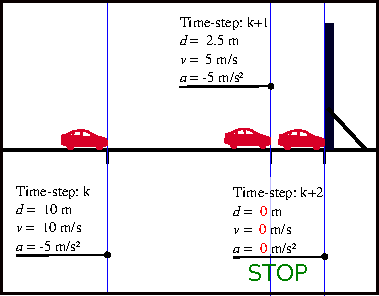
\includegraphics[width=0.7\linewidth]{\figurepath/car_example_2}
\caption{Braking phase for the car in scenario 1 as it stops before hitting the wall.}
\label{fig:car_example_2}
\end{figure}
Scenario 2: On a straight line, a second car is also  cruising towards the wall. Its current velocity is $v=10~m/s$, its distance to the wall is $d=10~m$ and its deceleration capability is $a_{m}=-1~m/s^2$. In its current state, none of the constraints\footnote{The constraint on its position ($d \geq 0$) and the constraint related to its deceleration capability ($a_m \leq a \leq a_M$).} of the car are violated. However, even if the vehicle starts \textit{braking} from time-step\footnote{For this example, the time-step duration is $1~s$.} $k$ using its full deceleration capability $a=a_{m}=-1~m/s$ (control input), collision with the wall is inevitable. Indeed, as shown in Fig.~\ref{fig:car_example_1}, during its braking phase, the car hits the wall between time-steps $k+1$ and $k+2$ and this, before bringing its velocity to $0$. In this case, it is said that: the constraint related to the deceleration capability of the car and the one on its position are \textit{incompatible}. At time-step $k+1$, there is no solution for the control problem that does not violate the car's constraints at the next time-step. \\
It is clear why there is no issue of constraints incompatibility for the vehicle in the first scenario as the amount of deceleration it can produce is larger than for the car in scenario 2, $-5~m/s^2$ compared to $-1~m/s^2$. A \labelText{{\color{red}\underline{solution}}}{label:solution} to ensure compatibility for the constraints of the vehicle in scenario 2 can be as follows: considering its low deceleration capability ($-1~m/s^2$), the black car in  Fig.~\ref{fig:car_example_1} should start \textit{braking} several time-steps in advance. Precisely, as shown in Fig.~\ref{fig:car_example_2}, $10$ time-steps before reaching the wall and $50~m$ from it. These are the needed time and distance to completely stop the vehicle considering an initial velocity of $v=10~m/s$. The only way to implement this solution is to reformulate the naive expression of the position related constraint to take into account the available deceleration capability $a_m$ in addition to the instantaneous state of the car plus the considered position limit: $f(d,v,a_{m})\geq 0$. With such a formulation, every time the vehicle reaches an \textit{extreme} state\footnote{An extreme state for the car is a state from which, considering its deceleration capability, if it starts braking using this maximum deceleration, it will stop just before hitting the wall.}, the reflected constraint on the control variable is automatically activated, a \textit{braking phase} is  implicitly engaged and a \textit{viable} \cite{aubin1991viability} solution is available for the control problem as the car copes with its position limit. 
\\
We recall the concept of \textit{viability} \cite{aubin2011viability} that is often used when dealing with the balance issue for humanoid robots. It can naturally be extended to the \textit{constraints incompatibility} problem \cite{fraichard2007short} as follows: \textit{A state is viable if starting from this state there exists over an infinite horizon of time a sequence of control inputs that satisfies all constraints in the future}. Therefore, considering the notion of \textit{viability}, unlike the state of the black car at time-step $k$ in scenario 1, the state of the red one in scenario 2 at the same time-step and for all the following time-steps is \textit{viable}. 
%\begin{landscape}
%\begin{figure}[!htbp]
%\centering
%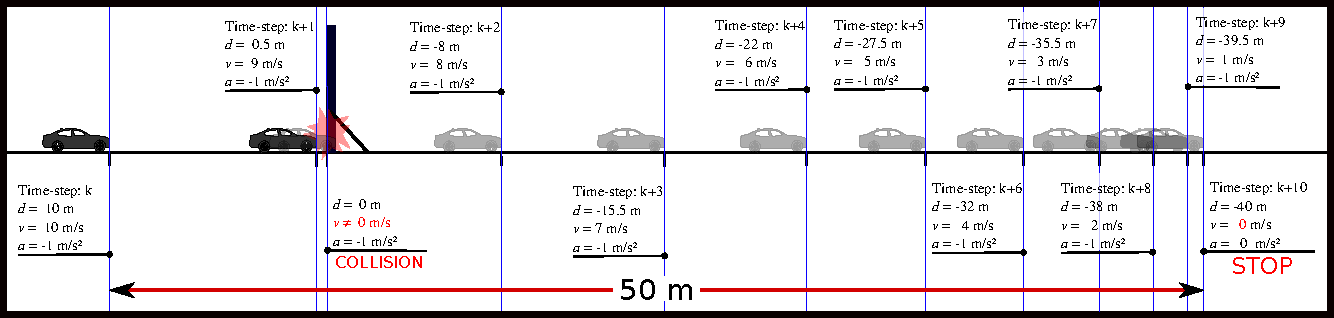
\includegraphics[width=0.99\linewidth]{\figurepath/car_example_1}
%\caption{Braking phase for the car in scenario 1 as it collides with the wall. Transparent frames show the continuation of the braking phase if the wall is removed.}
%\label{fig:car_example_1}
%\end{figure}
%\begin{table}[]
%\centering
%\begin{tabular}{|c|l|c|c|c|l|c|c|}
%\hline
%\multicolumn{4}{|c|}{Articular space constrains} & \multicolumn{4}{c|}{Operational space constraints} \\ \hline
%\multicolumn{2}{|c|}{\multirow{2}{*}{\begin{tabular}[c]{@{}c@{}}Type 1:\\ static constraints\\ $S \leq S_M$\end{tabular}}} & \multicolumn{2}{c|}{\begin{tabular}[c]{@{}c@{}}Dynamic constraints\\ $S \leq \~S_M$\end{tabular}} & \multicolumn{2}{c|}{\multirow{2}{*}{\begin{tabular}[c]{@{}c@{}}Type 4:\\ Static constraints\\ $g(S) \leq g_M$\end{tabular}}} & \multicolumn{2}{c|}{\begin{tabular}[c]{@{}c@{}}Dynamic constraints\\ $g(S) \leq \~g_M$\end{tabular}} \\ \cline{3-4} \cline{7-8} 
%\multicolumn{2}{|c|}{} & \begin{tabular}[c]{@{}c@{}}Type 2:\\ Predictable limit\\ $\~S_M$\end{tabular} & \begin{tabular}[c]{@{}c@{}}Type 3:\\ Non predictable limit\\ $\~S_M$\end{tabular} & \multicolumn{2}{c|}{} & \begin{tabular}[c]{@{}c@{}}Type 5:\\ Predictable limit\\ $\~g_M$\end{tabular} & \begin{tabular}[c]{@{}c@{}}Type 6:\\ Non predictable limit\\ $\~g_M$\end{tabular} \\ \hline
%\end{tabular}
%\caption{Types of constraints that can be encountered when using a reactive controller. $S=\{\vect{q}, \vect{\dot{q}}\}$ is the state of the robot in articular space. $g(S)$ is the mapping of this state in operational space.}
%\label{my-label}
%\end{table}
%\end{landscape}
\begin{landscape}
\begin{figure*}
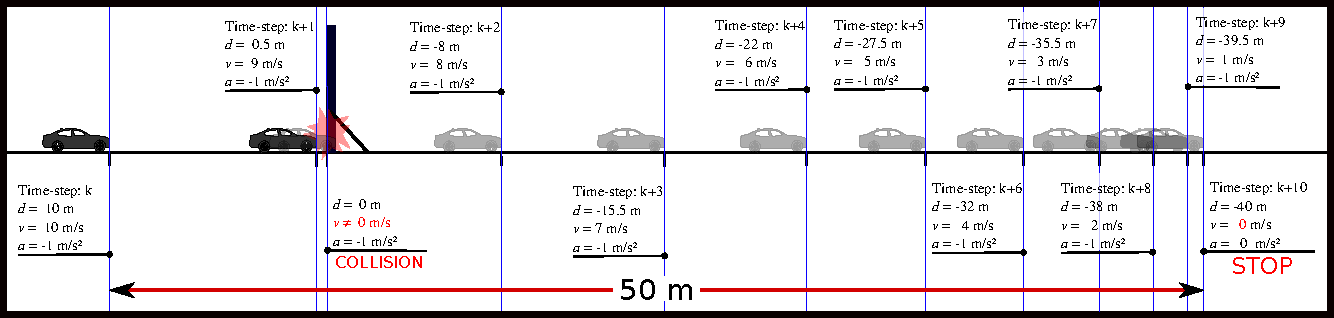
\includegraphics[width=1\linewidth]{\figurepath/car_example_1}
\caption{Braking phase for the car in scenario 2 as it collides with the wall. Transparent frames show the continuation of the braking phase in case the wall is removed.}
\label{fig:car_example_1}
\end{figure}
\begin{table}[]
\begin{center}
\begin{tabular}{|c|l|c|c|c|l|c|c|}
\hline
\multicolumn{4}{|c|}{Articular space constrains} & \multicolumn{4}{c|}{Operational space constraints} \\ \hline
\multicolumn{2}{|c|}{\multirow{2}{*}{\begin{tabular}[c]{@{}c@{}}Type 1:\\ static constraints\\ $S \leq S_M$\end{tabular}}} & \multicolumn{2}{c|}{\begin{tabular}[c]{@{}c@{}}Dynamic constraints\\ $S \leq \~S_M$\end{tabular}} & \multicolumn{2}{c|}{\multirow{2}{*}{\begin{tabular}[c]{@{}c@{}}Type 4:\\ Static constraints\\ $w(S) \leq w_M$\end{tabular}}} & \multicolumn{2}{c|}{\begin{tabular}[c]{@{}c@{}}Dynamic constraints\\ $w(S) \leq \~w_M$\end{tabular}} \\ \cline{3-4} \cline{7-8} 
\multicolumn{2}{|c|}{} & \begin{tabular}[c]{@{}c@{}}Type 2:\\ Predictable limit\\ $\~S_M$\end{tabular} & \begin{tabular}[c]{@{}c@{}}Type 3:\\ Non predictable limit\\ $\~S_M$\end{tabular} & \multicolumn{2}{c|}{} & \begin{tabular}[c]{@{}c@{}}Type 5:\\ Predictable limit\\ $\~w_M$\end{tabular} & \begin{tabular}[c]{@{}c@{}}Type 6:\\ Non predictable limit\\ $\~w_M$\end{tabular} \\ \hline
\end{tabular}
\caption{Types of constraints encountered when using a reactive controller. $S=\{\vect{q}, \vect{\dot{q}}, \vect{\ddot{q}}, \vect{\dddot{q}}\}$ is the extended state of the robot in articular space. $w(S)=\{\vect{X}, \vect{\dot{X}}, \vect{\ddot{X}}, \vect{\dddot{X}}\}$ is the mapping of this state in operational space.}
\label{my-label}
\end{center}
\end{table}
\end{landscape}
\subsection{Different types of constraints}
For reactive control schemes, types of constraints that can be encountered are summarized in table~\ref{my-label}. We distinguish two groups of constraints: 1) articular space constraints that concern directly the extended state of the robot $S=\{\vect{q}, \vect{\dot{q}}, \vect{\ddot{q}}, \vect{\dddot{q}}\}$. For example, the constraints related to an actuator's position and velocity limits. And 2) operational space constraints usually expressed as non-linear functions of $S$ and that relate to the movements of the robot in operational space. For example, a constraint of keeping a safe distance $d_{safe}$ between the robot and an obstacle within its workspace. Such constraint can, independently from other constraints, be expressed: 
\begin{equation}
\underbrace{\left(J_{c}(\vect{q}) \vect{\dot{q}}\right) }_{\dot{X}} \vec{\vect{n}} \hspace{1mm}\delta t + d \geq d_{safe},
\label{eq:bat_coll}
\end{equation}
where $J_c$ is the Jacobian matrix associated to the closest part from the structure of the robot to the obstacle, $\vec{\vect{n}}$ is the vector associated to the shortest distance between the obstacle and the robot, $\vect{\dot{q}}$ is the generalised articular velocity, $\delta t$ is the control sample-time and $d$: the instantaneous closest distance between the robot and the considered obstacle.
\\
As shown in table~\ref{my-label}, constraints from the two groups are either static or dynamic. A static constraint is a constraint which limit is constant and does not variate over time, for example, a physical position limit for an actuator. On the other hand, dynamic constraints are formulated with limits that can change in time, for example based on sensory acquired data. Variations of these limits can be either: 1) predictable, for example, a constraint of keeping a safe distance between the robot and an obstacle entering its workspace with a \textit{constant} velocity, 2) non-predictable, like the movement of a human-operator nearby the robot. The variation of the distance between the robot and the person cannot easily be predicted. \\
To prevent a robot from getting into \textit{non-viable} states, all its constraints must be reformulated to include the reaction capabilities of its actuators, namely: the max/min producible articular deceleration/torque and jerk. Analogue to the cars in scenarios 1 and 2, coping with a constraint implies a braking phase that is implicitly induced by the actuators of the robot. The span of such braking phase depends on the system's dynamic capabilities. Therefore, each constraint in table~\ref{my-label}, expressed with its naive formulation, can be compatible with the reaction capabilities of the robot in case of actuators that can produce infinite torque/deceleration and jerk. In such case, the duration of the implicitly induced braking phases can be reduced to \textbf{one} control sample-time. \\
The naive expressions of constraints in table~\ref{my-label} can be modified as follows:\\
For type 1 constraints, just as the suggested \nameref{label:solution} for the black car in scenario 2, considering constant articular  deceleration and jerk capabilities\footnote{Which is not exactly the case for multi-body robots.} and a static limit $S_M$, a \textit{formal} solution to the control problem that preserves \textit{viability} for the state of the robot can be computed. For this, the formulation of this type of constraints must be modified to take into account the system's articular reaction capabilities, namely, producible articular deceleration $[\vect{\ddot{q}}_m, \vect{\ddot{q}}_M]$ and jerk $[\vect{\dddot{q}}_m, \vect{\dddot{q}}_M]$. The same can also be done in case of constraints with dynamic predictable limits $\~S_M$ (type 2). Considering an accurate prediction, such bounds can be handled as static limits. For type 3 constraints, a straight forward solution is to widely bound the variations of the dynamic limit $\~S_M$, which can however substantially alter the optimality of the control solution regarding the task to perform. A type 3 constraint can be for example a constraint on the kinetic energy of the robot expressed in articular space. Such constraint can be formulated: $\frac{1}{2} M(\vect{q}) \vect{\dot{q}}^2 \leq E_c^{art}$, with $E_c^{art}$ the maximum allowed kinetic energy in articular space. When reflected on $\vect{\dot{q}}$, the constraint is written: $\vect{\dot{q}} \leq \sqrt{2 M(\vect{q})^{-1}E_c^{art}}$. The problem with constraints of type 4 is, even if the reaction capabilities of the robot in joint space can be considered constant, the non-linear and configuration dependent mapping\footnote{$[\vect{\ddot{q}}_m, \vect{\ddot{q}}_M], [\vect{\dddot{q}}_m, \vect{\dddot{q}}_M] \rightarrow [\vect{\ddot{X}}_m, \vect{\ddot{X}}_M], [\vect{\dddot{X}}_m, \vect{\dddot{X}}_M]$.} of these performances into operational space renders the estimation of the braking capabilities in Cartesian space impossible without predicting the future movements of the robot. Consequently, coping \textit{properly} with a static limit in Cartesian space is more complex. And it is even more for dynamic constraints (type 5 and type 6). A type 4 constraint can be for example a constraint on the operational velocity of the end-effector of a robotic manipulator. Such constraint can be expressed: $\vect{\dot{X}} = J(\vect{q}) \vect{\dot{q}} \leq \vect{\dot{X}}_M$, with $\vect{\dot{X}}_M$ the maximum allowed velocity for the end-effector in Cartesian space. A type 6 constraint can be for example a constraint on the operational velocity of end-effector of the robot but with a maximum allowed limit that depends on the instantaneous distance to a considered approaching obstacle. 
%This forecast of its future articular configurations as it brakes to cope with the considered constraints is important so the reaction capabilities in Cartesian space are guaranteed.
%For a constraint of type 1, just as the proposed solution for the car in scenario 1, to ensure viability, a formal solution that takes into account the articular\footnote{Considered constant.} reaction capabilities of the robot can be computed for the control problem; And this, in case the limit of the constraint is static or if it can be precisely predicted (type 2). DependiFng on these capabilities, the reflected constraint on the control input will be activated at the right time. \\
%For a type 3 constraint, a naive solution will be to widely bound the variations of its limit. This will however alter the optimality of the solution. The problem with constraints of type 4 is, even if the articular reaction capabilities can be considered constant\footnote{Which is not exactly the case for the articular deceleration and jerk capabilities.} in joint space, the non-linear and configuration dependent mapping of these performances in operational space makes the estimation of the braking profile impossible without any prediction on the future movements of the robot. Coping exactly with the static limit becomes a difficult task. Which is even more complex for dynamic constraints (type 5 and type 6).      
%In both articular and operational spaces, we distinguish static and dynamic constraints. A static constraint is a constraint which limit is constant and does not variate over time. On the other hand, dynamic constraints are formulated with limits that can change in time (for e.g. depending on sensory acquired data). 
%
%a constant limit in operational space corresponds actually to a dynamic one in articular space. This is due to the non-linear and configuration dependent mapping between the two domains. For example, a constraint of non-collision between the    
%%%%%%%%%%%%%%%%%%%%%%%%%%SUBSECTION%%%%%%%%%%%%%%%%%%%%%%%%%%%%%
%%%%%%%%%%%%%%%%%%%%%%%%%%%%%%%%%%%%%%%%%%%%%%%%%%%%%%%%%%%%%%%%%
%%%%%%%%%%%%%%%%%%%%%%%%%%SUBSECTION%%%%%%%%%%%%%%%%%%%%%%%%%%%%%
\subsection{Corresponding literature}
\label{subsec:crspnd_litt}
The problem of \textit{constraints incompatibility} in this chapter is tackled for constraints related to the articular position and velocity limitations of a robotic manipulator. Therefore, the brief state-of-the-art presented hereby is exclusive to the same type of constraints: (type 1 in table~\ref{my-label}). \\
The issue of \textit{constraints incompatibility} is studied in the literature since a long time and remains an open one. In \cite{park1998enhanced}, the problem of high peak of torque and chattering phenomena on the movement of the actuator is highlighted when a joint angle limit of a serial robot is reached. This results from decelerating the limiting joint in order to stop its motion in one sampling time. The following problems appear:
\begin{enumerate}
\item collision with the joint angle limit when no sufficient control torque and/or jerk capabilities are available.
\item vibrations by exciting hidden resonant modes of the manipulator which can lead to instability.
\end{enumerate}
Park et al. in \cite{park1998enhanced} use a method called \textit{P-Step-Ahead Predictor (PSAP)}. Articular position and velocity limits are  detected far earlier and the braking phases are activated $p$ time-steps in advance to reduce the required amount of torque. In addition, the modulation of a weighting matrix related to the manipulability measure \cite{yoshikawa1985manipulability} is used simultaneously for the same purpose. The problem with this proposed approach is the inevitable heuristic trial and error method to fix the acting parameters (e.g., $p$). Decr\'e et al. in \cite{decre2009extending} were the first to  formulate a mathematical solution to directly integrate the deceleration capabilities of a serial robot into the expression of a Cartesian position constraint aimed to keep the end-effector of a robot at a specific distance from the considered obstacle. Which results into a smoother articular velocity control input. Rubrecht et al. in \cite{rubrecht2010constraints} extend the idea to the constraints related to the articular limitations of a robotic manipulator. The deceleration capabilities are included in the formulation of the articular position constraint, that is then automatically activated $n$ time-steps before the joint position boundaries. However, only kinematic-level control is considered in their work. Lange in \cite{lange2014predictive} and  \cite{lange2015trajectory} use a scaling method to generate an immediate Path-Accurate and Jerk-Limited stopping motion for industrial robots. This method can at first glance be transposed and used when coping with articular limitations related constraints. The optimal time for triggering the stopping motion needs however to be computed.  \\

Besides these formal methods that have been proposed to solve the problem of constraints incompatibility, other techniques that are based on Optimal Control approaches seem well suited for handling that problem. Indeed, Optimal Control provides a systematic approach to optimally compute the control input so as to best track the control objectives while accounting for the current and future constraints on the control inputs and states of a system. As a matter of fact, to be able to guarantee the viability\footnote{As redefined as the very end of section 2.1.1.} of the state of the robot with respect to its articular constraints but also with respect to operational ones, the control problem should not be solved reactively but over an infinite horizon of time under these strict and explicit constraints.

Nevertheless, reasoning and solving the control problem over an infinite horizon of time does not make much sense in very dynamic environments and contexts where the tasks to be performed are defined and adapted on-line. This advocates for online Optimal Control approaches where the horizon of control input is recomputed at each control time step. However this comes at a very high price as it requires to employ a model of the system's dynamics in order to preview its behaviour over time and compute an optimal horizon of control inputs that maintain the system into a valid state space. It therefore requires a time-integration of the local system model which generally leads to costly non-linear and non-convex optimisation problems \cite{2016THDR3834}. In practice, to address this complexity problem, the time horizon can be reduced to some appropriate value. This falls in the category of Model Predictive Control where the Optimal Control problem is solved for a given receding horizon. While this reduces the computation cost, the latter remains high and one way to simplify it further is to use a reduced model of the system's dynamics in order to render the MPC problem simpler to solve. This approach has seen a lot of developments in the control of balance for humanoid robots where the dynamics of balancing are reduced to some more or less complex inverted pendulum control problem. This simplified model is used to compute, over a receding horizon, the desired acceleration of the center of mass of the robot given some path to follow and some balance constraints \cite{wieber2006trajectory}, \cite{ibanez2015Emergence}. While this model reduction approach leads to great results, it also implies a suboptimal use of the dynamics of the robot. Furthermore, the reduced model cannot not incorporate joint space variables which makes it impossible to actually account for very low-level constraints such as joint position limits or input torque saturation. 

MPC approaches are therefore gradually extended to control with the consideration of models capturing the system state at the joint level. Computational limitations nevertheless requires the setup of simplifications of the control problem. A significant improvement in this direction is performed by Y. Tassa et al.. in \cite{tassa2012synthesis}. The authors address computational issues in two ways in this work. First, the resolution of the MPC optimisation problem is considered over the whole duration of the activity. That is, the control problem solely aims at continuously driving the system towards an all-time minimum, rather than finding an optimum at each control step. To this aim a suboptimal solution solely is demanded at each control step, generally obtained through a single iteration of the optimisation algorithm. It therefore allows the consideration of much more complex optimisation problems. In this particular work, an iterative Linear Quadratic Gaussian optimiser, a variant of Differential Dynamic Programming, is setup to work over the joint actuation space. Computational issues nevertheless arise from the needs to update the model rapidly for an iteration of the optimiser. To meet this challenge, the second contribution of this work is thus to propose a fast dynamics integrator. However this controller still requires a large time slowdown with optimisation iterations of 140ms, thus forbidding a direct real-time implementation. The MPC problem is employed as a trajectory generator running slower than the rate of the lower, tracking control loop. This cannot be considered as satisfactory in terms of constraint compatibility but still provides an interesting step toward a general approach to this problem.

In this work, a different type of solution is explored and the choice is explicitly made to follow a formal approach, trying to exploit as much as possible formal compatibilisation of joint level imbricated constraints. The clear goal of such an approach is clearly to provide a very reactive way of keeping track of viability thus ensuring an optimal use of the system's dynamic capabilities.
%Besides these formal methods that have been proposed to solve the problem of \textit{constraints incompatibility}, other techniques that are based on Model Predictive Control (MPC) seem well suited for handling \textit{constraints incompatibilities}. Indeed, MPC provides a systematic approach to account for the current and future constraints on the control inputs and states of a system. In robotics, MPC is usually used as a common optimal approach for balance regulation. It employs a model of the system dynamics to preview its behaviour over time and compute an optimal horizon of control inputs that maintain the system into a valid state space. It requires therefore a time-integration of the local system model which generally leads to non-linear and non-convex optimisation problems \cite{ibanez:tel-01308723}. The formulation of the problem of \textit{constraints incompatibility} for constraints related to the physical articular limitations  of a robot controlled at the dynamic-level using MPC can be as:
%\begin{equation}
%\begin{split}
%\tau_{M}^c =\hspace{1mm} &\text{maximize  } \hspace{2.5mm}\tau_{|k}^c, \\
%&\text{subject to : }  S_{m_{|k}} \leq S_{|k} \leq S_{M_{|k}} \hspace{3mm} \forall k \in [0:\infty],
%\end{split}
%\label{eq:qddot_minimizkio}
%\end{equation}
%with $\tau^c$  the control torque input and $\tau_{M}^c$ its upper bound. $S_{|k}$, $S_{m_{|k}}$ and $S_{M_{|k}}$ are respectively the extended state of the robot expressed in articular space and its lower and upper bounds at control time-step $k$. The lower bound $\tau_{m}^c$ can similarly be computed by minimizing $\tau_{|k}^c$ rather than maximizing it. \\
%To be able to guarantee the \textit{viability}\footnote{As redefined in Section~\ref{sec:gen_prblm}.} of the state of the robot vis-a-vis its articular constraints, the problem described in (\ref{eq:qddot_minimizkio}) must be solved for an infinite horizon of time. However, computational limitations require the setup of simplifications of the control problem as time-integration is one of the major challenges of MPC formulations. A sliding finite horizon MPC strategy can then be preferred \cite{tan:tel-01310675}.
%A significant improvement in this direction was performed by Y. Tassa et al. in \cite{tassa2012synthesis} where the computational issues are addressed partially by considering the resolution of the MPC optimisation problem over just the whole duration of the activity instead of an infinite horizon of time.
%
%Because of these various limitations when using MPC and as a \textit{\textbf{formal}} solution to the \textit{constraints incompatibility} problem exist and can optimally be computed (especially regarding the constraints related to the physical articular limitations of a robotic manipulator). It is therefore the formal approach that is used in this chapter to resolve this problem for robots that are controlled at the dynamic-level.
%%%%%%%%%%%%%%%%%%%%%%%%%%SUBSECTION%%%%%%%%%%%%%%%%%%%%%%%%%%%%%
%%%%%%%%%%%%%%%%%%%%%%%%%%%%%%%%%%%%%%%%%%%%%%%%%%%%%%%%%%%%%%%%%
%%%%%%%%%%%%%%%%%%%%%%%%%%SUBSECTION%%%%%%%%%%%%%%%%%%%%%%%%%%%%%
\subsection{Contributions}
In this work, the problem of \textit{constraints incompatibility} is solved for constraints of type 1 and precisely for robots controlled at the dynamic-level. The constraints on articular positions, velocities, accelerations and jerk are expressed as inequalities within a QP formulation of a reactive control problem. The main contribution concerns the mathematical reformulation of the following constraints:
\begin{itemize}
\item no violation of joint position bounds;
\item no violation of joint velocity bounds.
\end{itemize}
To avoid incompatibility problems when reactively coping with such constraints, the new proposed formulations that are expressed at the dynamic-level take into account the reaction capabilities, i.e., the articular deceleration and jerk producible by the actuators of the robot. One kind of incompatibility can occur for example when a braking phase is implicitly induced by the actuators of the robot to stop the movement of a joint at a static position limit within a short period of time, for e.g., one control time-step. This requires high deceleration and jerk capabilities the robot may not be able to produce. Indeed, to be optimal, a robotic system must take the highest advantage from its dynamic capabilities within its limiting ranges; for example, to be as close as possible to a maximum allowed position with high articular acceleration and velocity and still be able to stop in time and not violate the considered limit. This can be achieved through a braking phase triggered $n$ time-steps before reaching the limit and that takes into account the system's limited available deceleration capabilities, i.e., the producible articular torque/deceleration and jerk. Every time an actuator reaches an \textit{extreme} state, with its new formulation, the constraint is activated and a braking phase is implicitly engaged at the right moment. In addition to the new formulations of the articular position and velocity constraints, that take into account the dynamic capabilities of the robot actuators. A method to compute the exact number $n$ of time-steps needed for the implicitly induced braking phases, triggered at the activation of the considered constraints, is introduced. The \textit{viability} of the state of the robot regarding the joint's position, velocity, acceleration/torque and jerk can then be guaranteed over an infinite horizon of time. \\
%In case of redundant manipulators, the control problem can either be formulated at the kinematic-level as the inversion of the following relation: 
%\begin{equation}
%\vect{\dot{X}} = J(\vect{q}) \dot{\vect{q}}
%\label{eq:vel_kin_opt}
%\end{equation}
%or at the torque-level when dynamic capabilities like contact forces control are needed: 
%\begin{equation}
%\vect{\ddot{X}} = \dot{J}(\vect{q}) \vect{\dot{q}} + J \ddot{\vect{q}}
%\label{eq:X_ddot}
%\end{equation}
%$J(\vect{q})$, $\vect{\dot{X}}$, $\vect{\ddot{X}}$, $\vect{\dot{q}}$, $\vect{\ddot{q}}$ are respectively the operational task Jacobian matrix, the operational velocity and acceleration vectors and the joint velocity and acceleration vectors.
%\\
%When it stills possible to implement constraints using an analytical scheme \cite{ngo2005passivity},\cite{ngo2006bounded}, the most general approach consists in formulating the control problem as a convex optimization one. Constraints are then expressed both through equalities and inequalities \cite{chen1994torque}-\cite{ma2002time}.
\\
The present chapter is organized as follows: In section 2, the reactive controller used to compare different formulations of the constraints on articular velocity and position is introduced. First, the naive formulations of these constraints are presented then, by studying the relation between the extended state of the robot $S=\{\vect{q}, \vect{\dot{q}}, \vect{\ddot{q}}\right), \vect{\dddot{q}}\}$ and the system's physical limitations: $[\vect{q}_m, \vect{q}_M]$, $[\vect{\dot{q}}_m, \vect{\dot{q}}_M]$, $[\vect{\ddot{q}}_m, \vect{\ddot{q}}_M]$, $[\vect{\dddot{q}}_m, \vect{\dddot{q}}_M]$, the different incompatibility cases that may occur are exposed. In section 3, the incompatibility cases are resolved and the new formulations of the joint velocity and position constraints that take into account the dynamic capabilities of the actuators of the robot are introduced. In section 4, the final bounds reflected on the dynamic control variable that allow coping with all a robotic manipulator's articular limitations at the same time are formulated. In section 5, the contributions are summarized, the encountered difficulties and the limitations of the proposed new formulation of constraints are highlighted. 
%In practical applications, a control strategy for a robotic system is usually formulated depending on the nature of the operational task to be performed. Two kinds of strategies are distinguished: a proactive one when the objective of the operational task is already known (e. g. moving the end-effector from point A to point B) and a reactive strategy when the input data for the operational task are not known a priori but discovered at every time-step (e.g., tele-operation, co-manipulation applications...etc.). 
%
%Independently from the control strategy, compliance to constraints and specifically to the physical constraints of the actuators is a must for any robotic system. This is particularly true in cases where constraints violation is highly critical (e.g., surgery, de-mining...etc.). 
%\\
%To ensure strict compliance, for proactive control strategies, constraints and tasks can be handled offline. For example, to move the end-effector from point A to point B in the Cartesian space, trajectories can be generated directly at the joint level. In this context, Katzschmann et. al in \cite{katzschmann2013towards} present a trajectory generating algorithm that takes into account the actuators max/min position, velocity, torque and even jerk capabilities. On the other hand, when tasks or constraints are not known in advance (reactive control cases), \textit{trajectories cannot be generated} and it becomes impossible to use the same approach to cope with articular limitations. In the presented work, this issue is solved for robots controlled at the dynamic-level. Constraints on articular positions, velocities, accelerations and jerk are expressed as inequalities within a QP formulation of the reactive control problem. The main contribution concerns the mathematical reformulation of the following constraints:
%\begin{itemize}
%\item No violation of joint position bounds.
%\item No violation of joint velocity bounds.
%\end{itemize}
%Within the new formulations, articular deceleration and jerk capabilities are integrated to avoid incompatibilities. One kind of incompatibilities can occur when inducing a braking phase to stop the movement of an actuator at a static\footnote{We distinguish two types of bounds/constraints: \begin{itemize}
%\item Static constraints: $x \leq x_{max}$ with: $x_{max}$ constant. 
%\item Dynamic constraints: $x \leq \~{x}_{max}(t)$ with: $\~x_{max}(t)$ varying over time.
%\end{itemize}
%}
%position limit within a short period of time, e.g., one control time-step. This requires high deceleration and jerk capabilities that the robot may not be able to produce. Indeed, to be optimal, a robotic system must take the highest advantage of its dynamic capabilities within its limiting ranges. For example, to be as close as possible to a maximum allowed position with high articular acceleration and velocity and still be able to stop at time and not violate the considered limit. This can be achieved through a braking phase triggered $n$ time-steps before reaching the limit and that takes into account the available deceleration capabilities of the system, namely: torque and jerk.  \\
%In case of redundant manipulators, the control problem can either be formulated at the kinematic-level as the inversion of the following relation: 
%\begin{equation}
%\vect{\dot{X}} = J(\vect{q}) \dot{\vect{q}}
%\label{eq:vel_kin_opt}
%\end{equation}
%or at the torque-level when dynamic capabilities like contact forces control are needed: 
%\begin{equation}
%\vect{\ddot{X}} = \dot{J}(\vect{q}) \vect{\dot{q}} + J \ddot{\vect{q}}
%\label{eq:X_ddot}
%\end{equation}
%$J(\vect{q})$, $\vect{\dot{X}}$, $\vect{\ddot{X}}$, $\vect{\dot{q}}$, $\vect{\ddot{q}}$ are respectively the operational task Jacobian matrix, the operational velocity and acceleration vectors and the joint velocity and acceleration vectors.
%\\
%When it stills possible to implement constraints using an analytical scheme \cite{ngo2005passivity},\cite{ngo2006bounded}, the most general approach consists in formulating the control problem as a convex optimization one. Constraints are then expressed both through equalities and inequalities \cite{chen1994torque}-\cite{ma2002time}. The issue of constraints compatibility exists since a long time and remains an open one. In \cite{park1998enhanced} the problem of high peak of torques and chattering phenomena is highlighted when the joint angle limit of a serial robot is reached. This results from decelerating the limiting joint in order to stop the motion in one sampling time. the following problems appear:
%\begin{enumerate}
%\item Collision with the joint angle limit when no sufficient control torque and/or jerk capabilities are available.
%\item Vibrations by exciting hidden resonant modes of the manipulator which can lead to instability.
%\end{enumerate}
%Park et al. in \cite{park1998enhanced} use a method called \textit{P-Step-Ahead Predictor (PSAP)}. Articular position and velocity limits are  detected far earlier and the braking phase is activated $p$ time-steps in advance to reduce the required amount of torque. In addition, the modulation of a weighting matrix related to the manipulability measure \cite{yoshikawa1985manipulability} can be used for the same purpose. The problem with the proposed approach is the inevitable heuristic trial and error method to fix the acting parameters (e.g., $p$). Decré et al. in \cite{decre2009extending} were the first to  formulate a mathematical solution to directly integrate the deceleration capabilities into the expression of a Cartesian position constraint; This resulted into a smoother articular velocity control input. Rubrecht et al. in \cite{rubrecht2010constraints} extended the idea to articular constraints. The deceleration capabilities  are integrated in the formulation of articular position constraints that are automatically activated $n$ time-steps before the joint position boundaries. Lange in \cite{lange2014predictive} and Suppa in \cite{lange2015trajectory} use a scaling method to generate an immediate Path-Accurate and Jerk-Limited stopping motion for industrial robots. This method can be transposed and used when coping with articular limits. The correct time for triggering the stopping motion needs however to be computed. 
%\\
%\\
%The organization of this chapter is as following: In section 2 we present the reactive controller that will be used to compare different formulations of articular constraints. We present the classic way used to formulate these constraints then, by studying the relationship between the joint parameters: $\vect{q}$, $\vect{\dot{q}}$, $\vect{\ddot{q}}$ and their corresponding limitations: $[\vect{q}_m, \vect{q}_M]$, $[\vect{\dot{q}}_m, \vect{\dot{q}}_M]$, $[\vect{\ddot{q}}_m, \vect{\ddot{q}}_M]$, $[\vect{\dddot{q}}_m, \vect{\dddot{q}}_M]$, we expose the different incompatibility cases that may occur. In section 3, the incompatibility cases are resolved and new formulations of velocity and position constraints that take into account the reaction capabilities of the robot are presented. 
%In section 4 we formulate the final bounds reflected on the control variable to cope with all the articular limits of the system at the same time. In section 5 we conclude and give more insights on the generalisation of the presented formulations for constraints expressed in the Cartesian space. 
%%%%%%%%%%%%%%%%%%%%%%%%%%%%%%%%%%%%%%%%%%%%%%%%%%%%%%%%%
      %The QP form and Constraints Compatibility%
%%%%%%%%%%%%%%%%%%%%%%%%%%%%%%%%%%%%%%%%%%%%%%%%%%%%%%%%%
\section[The QP form and the different constraints incompatibility cases]{The QP form and the different constraints incompatibility cases}
This section aims at establishing the general formulation of the constrained, redundant dynamic reactive control scheme. The objective is to compute every  time-step the control torque $\boldsymbol{\tau}_{|k}^{c}$ in order to perform a trajectory tracking task in joint space while coping at the same time with the articular position, velocity, torque/acceleration and jerk constraints. We highlight the fact that, desired trajectories for the joints of the robot are not known in advance but \textit{discovered at every time-step} (tele-operation analogue situation). Incompatibility cases related to the naive way of expressing the articular constraints are exposed and discussed. 
%%%%%%%%%%%%%%%%%%%%%%%%%%SUBSECTION%%%%%%%%%%%%%%%%%%%%%%%%%%%%%
%%%%%%%%%%%%%%%%%%%%%%%%%%%%%%%%%%%%%%%%%%%%%%%%%%%%%%%%%%%%%%%%%
%%%%%%%%%%%%%%%%%%%%%%%%%%SUBSECTION%%%%%%%%%%%%%%%%%%%%%%%%%%%%%
\subsection{Task formulation}
The objective function of the controller is defined as an error to be minimized. A joint-space acceleration task is considered and the error is between the desired articular acceleration $\vect{\ddot{q}}^{~des}$ and the expected acceleration $\vect{\ddot{q}}^{c}$; $\vect{\ddot{q}}^{~des}$ is computed:
\begin{equation}
\vect{\ddot{q}}_{|k}^{~des} = K_p (\vect{q}_{|k}^{*}-\vect{q}_{|k}) - K_d \vect{\dot{q}}_{|k}^{*}, 
\label{qddot}
\end{equation}
where $K_p$, $K_d$ $\in \mathbb{R}^{+}$ are the proportional and derivative gains.
%
%It is written in function of the control input $\vect{\tau}_{|k}^{c}$:
%\begin{equation}
% \vect{\ddot{X}}^{c} = J(\vect{q}) M(\vect{q})^{-1} \left(\boldsymbol{\tau}_{|k}^{c} - \vect{b}(\vect{q},\vect{\dot{q}})\right) + \dot{J}(\vect{q}) \vect{\dot{q}}
%\label{Xddot}
%\end{equation}
%$\vect{b}(\vect{q},\vect{\dot{q}})$ are the non linear terms, namely gravity, Coriolis and centrifugal induced generalized forces. $M(\vect{q})$ is the joint space inertia matrix of the robot. $\vect{\ddot{X}}^c$ can be computed with a PD controller to track a desired trajectory (position $\vect{X}(t)^\star$ and velocity  $\vect{\dot{X}}(t)^\star$, \textit{discovered at every time-step}). 
The acceleration task function to be minimized is written:
\begin{equation}
\vect{g}(\vect{\ddot{q}}_{|k}^{c}) = \vect{\ddot{q}}_{|k}^{~des}-\vect{\ddot{q}}_{|k}^c.
\label{artaccelerationError}
\end{equation}
%%%%%%%%%%%%%%%%%%%%%%%%%%SUBSECTION%%%%%%%%%%%%%%%%%%%%%%%%%%%%%
%%%%%%%%%%%%%%%%%%%%%%%%%%%%%%%%%%%%%%%%%%%%%%%%%%%%%%%%%%%%%%%%%
%%%%%%%%%%%%%%%%%%%%%%%%%%SUBSECTION%%%%%%%%%%%%%%%%%%%%%%%%%%%%%
\subsection{Controller formulation}
\label{subsec:cntrl_frm}
The proposed control strategy computes the control torque by minimizing the norm of the articular acceleration task function expressed in the following quadratic form: 
\begin{equation}
\argmin \limits_{\boldsymbol{\tau}_{|k}^{c}, \vect{\ddot{q}}_{|k}^{c}}  \left\| \vect{g}\left(\vect{\ddot{q}}_{|k}^{c}\right) \right\|_{Q_t}^2 + \epsilon  \| \boldsymbol{\tau}_{|k}^{c} \|_{Q_r}^2,
\label{eq:ctrl_pb}
\end{equation}
subject to:
\begin{equation}
M(\vect{q}_{|k}) \vect{\ddot{q}}_{|k}^{c} + \vect{b}(\vect{q}_{|k},\vect{\dot{q}}_{|k}) = \vect{\tau}_{|k}^{c},
\label{eq:dyn_eq}
\end{equation}
%subject to (\ref{eq:qddot_FINAL_CONSTR_1}) and (\ref{eq:qddot_FINAL_CONSTR_2}).
\\
with $\vect{\ddot{q}}_{|k}^{c}$ and $\vect{\tau}_{|k}^{c}$: the optimization control variables.
$\vect{b}(\vect{q}_{|k},\vect{\dot{q}}_{|k})$ are the non linear terms, namely gravity, Coriolis and centrifugal induced generalized forces. $M(\vect{q}_{|k})$ is the joint space inertia matrix of the robot. $Q_t$ and $Q_r$ are  positive semi-definite weighting matrices and $\| \vect{a} \|_{Q}$ is the $Q-$weighted euclidean norm of $a$. $\epsilon  \| \boldsymbol{\tau}_{|k}^{c} \|_{Q_r}^2$ with $\epsilon << 1$ serves as a regularization task in order to ensure the uniqueness of the control solution and to minimize the norm of the computed control torque.\\
It can be shown that the quadratic forms composing the tasks can be written as functions of positive semi-definite matrices. This LQP optimization problem is therefore convex and admits a unique global solution \cite{boyd2004}. 
\\ 
In addition to the equality constraints corresponding to the dynamic equation \eqref{eq:dyn_eq}, the problem is also subject to inequality constraints described in the upcoming sections. 
%
%\section{The QP form and articular constraints incompatibility cases}
%This section aims at establishing the general formulation of the constrained, redundant dynamic reactive control scheme. The objective is to compute the control torque $\boldsymbol{\tau}_{|k}^{c}$ in order to perform a trajectory tracking task in joint space while coping at every time-step with articular position, velocity, acceleration and jerk constraints. We highlight the fact that in this particular case the desired trajectories for the joint of the robot are \textit{discovered at every time-step} (tele-operation analogue situation) and are not known in advance. Incompatibility cases related to the classic way of expressing articular constraints are discussed. 
%\subsection{Task formulation}
%The objective function of the controller is defined as an error to be minimized. A joint-space acceleration controller is considered and the error is between the expected acceleration $\vect{\ddot{q}}^c$ and the real acceleration $\vect{\ddot{q}}$ of the robot's end-effector. It is written in function of the control input $\vect{\tau}_{|k}^{c}$:
%\begin{equation}
% \vect{\ddot{X}}^{c} = J(\vect{q}) M(\vect{q})^{-1} \left(\boldsymbol{\tau}_{|k}^{c} - \vect{b}(\vect{q},\vect{\dot{q}})\right) + \dot{J}(\vect{q}) \vect{\dot{q}}
%\label{Xddot}
%\end{equation}
%$\vect{b}(\vect{q},\vect{\dot{q}})$ are the non linear terms, namely gravity, Coriolis and centrifugal induced generalized forces. $M(\vect{q})$ is the joint space inertia matrix of the robot. $\vect{\ddot{X}}^c$ can be computed with a PD controller to track a desired trajectory (position $\vect{X}(t)^\star$ and velocity  $\vect{\dot{X}}(t)^\star$, \textit{discovered at every time-step}). The acceleration task function to be minimized is written:
%\hspace{-2mm}
%\begin{equation}
%\resizebox{.911\hsize}{!}{$\vect{g}\left(\boldsymbol{\tau}_{|k}^{c},\vect{\ddot{X}}^c\right) =  \vect{\ddot{X}}^c - \left(J(\vect{q}) M(\vect{q})^{-1} \left(\boldsymbol{\tau}_{|k}^{c} - \vect{b}(\vect{q},\vect{\dot{q}}) \right) + \dot{J}(\vect{q}) \vect{\dot{q}}\right)$}
%\label{accelerationError}
%\end{equation}
%\subsection{Controller formulation}
%The proposed control strategy computes the control torque by minimizing the norm of the  Cartesian acceleration task function expressed in the following quadratic form: 
%\begin{equation}
%\argmin \limits_{\boldsymbol{\tau}_{|k}^{c}}  \left\| \vect{g}\left(\boldsymbol{\tau}_{|k}^{c},\vect{\ddot{X}}^c\right) \right\|_{Q_t}^2 + \epsilon  \| \boldsymbol{\tau}_{|k}^{c} \|_{Q_r}^2,
%\label{eq:ctrl_pb}
%\end{equation}
%%subject to (\ref{eq:qddot_FINAL_CONSTR_1}) and (\ref{eq:qddot_FINAL_CONSTR_2}).
%\\
%$Q_t$ and $Q_r$ are  positive semi-definite weighting matrices and $\| \vect{a} \|_{Q}$ is the $Q-$weighted euclidean norm of $a$. $\epsilon  \| \boldsymbol{\tau}_{|k}^{c} \|_{Q_r}^2$ with $\epsilon << 1$ serves as a regularization task in order to ensure the uniqueness of the control solution and to minimize the norm of the computed control torque. It can be shown that the quadratic forms composing the tasks can be written as functions of positive semidefinite matrices. This LQP optimization problem is therefore convex and admits a unique global solution. 
%$\vect{\ddot{q}}_{|k}^{c}$ and $\vect{\tau}_{|k}^{c}$ are the control optimization variables: 
%\begin{equation}
%M(\vect{q}) \vect{\ddot{q}}_{|k}^{c} + \vect{b}(\vect{q},\vect{\dot{q}}) = \vect{\tau}_{|k}^{c}
%\label{eq:dyn_eq}
%\end{equation}
%\\ 
%In addition to the equality constraints corresponding to the dynamic equation \eqref{eq:dyn_eq}, the problem is also subject to inequality constraints described in the upcoming sections. 
%%%%%%%%%%%%%%%%%%%%%%%%%%SUBSECTION%%%%%%%%%%%%%%%%%%%%%%%%%%%%%
%%%%%%%%%%%%%%%%%%%%%%%%%%%%%%%%%%%%%%%%%%%%%%%%%%%%%%%%%%%%%%%%%
%%%%%%%%%%%%%%%%%%%%%%%%%%SUBSECTION%%%%%%%%%%%%%%%%%%%%%%%%%%%%%
\subsection{Articular constraints: naive formulations}
First, we introduce some notations that will be used throughout the manuscript:
\begin{itemize}
\item t $\in \mathbb{R}^{+}$ denotes time;
\item $k \in \mathbb{N}$ denotes the current discrete time-step;
\item $\delta t$ is the time-step duration of the discrete-time controller;
\item $\textit{S}_{|k}=\{\vect{q}_{|k}, \vect{\dot{q}}_{|k}, \vect{\ddot{q}}_{|k}, \vect{\dddot{q}}_{|k}\}$ is the extended state of the system at the current time-step $k$ describing its joint position, velocity, acceleration and jerk;
\item $[\vect{q}_{M}, \vect{q}_{m}]$ are the max/min joint position boundaries;
\item $[\vect{\dot{q}}_{m}, \vect{\dot{q}}_{M}], [\vect{\ddot{q}}_{m}, \vect{\ddot{q}}_{M}], [\vect{\dddot{q}}_{m}, \vect{\dddot{q}}_{M}]$ are the joint velocity, acceleration and jerk boundaries.
\end{itemize}
A naive satisfaction of the constraints related to these boundaries can be stated as: the computed control input $\boldsymbol{\tau}_{|k}^{c}$ at instant $k$ must be such that the articular limits are not violated at the next time-step $k+1$. These constraints can naturally be expressed in form of inequalities:
\begin{subequations}
\label{eq:const_1_literature}
\begin{empheq}[left={}\empheqlbrace]{align}
\vect{q}_{m} & \leq \vect{q}_{|k+1}\leq \vect{q}_{M},\label{eq:cnt_lit_1}\\
\vect{\dot{q}}_{m} & \leq \vect{\dot{q}}_{|k+1} \leq \vect{\dot{q}}_{M},\label{eq:cnt_lit_2}\\    
\vect{\ddot{q}}_{m} & \leq \vect{\ddot{q}}_{|k}^{c}\hspace{4mm}\leq \vect{\ddot{q}}_{M},\label{eq:cnt_lit_3}\\
\boldsymbol{\tau}_{m} & \leq \boldsymbol{\tau}_{|k}^{c}\hspace{4mm}\leq \boldsymbol{\tau}_{M},\label{eq:cnt_lit_4}\\
\vect{\dddot{q}}_{m}  & \leq \vect{\dddot{q}}_{|k+1}\leq \vect{\dddot{q}}_{M}.\label{eq:cnt_lit_5}
\end{empheq}
\end{subequations}
With $\boldsymbol{\ddot{q}}_m$ and $\boldsymbol{\ddot{q}}_M$ that can be computed as in Appendix~\ref{app:constrcomp}.
\\
To be easily accounted for, these constraints can be expressed in function of the control variable $\vect{\ddot{q}}_{|k}^{c}$. Considering the literature \cite{rubrecht2010constraints}, \cite{decre2009extending}, the classic approach to do that is based on the extended state of the system at instant $k$ and a local discrete linear approximation of its behaviour within a $\delta t$ time-step duration:  
%\begin{equation} 
%\left\{\begin{array}{l}
%\begin{split}
%\vect{q}_{|k+1} & = \vect{q}_{|k} + \delta t \vect{\dot{q}}_{|k} + \frac{\delta t^{2}}{2} \vect{\ddot{q}}_{|k},\\
%\vect{\dot{q}}_{|k+1} &  =  \vect{\dot{q}}_{|k} + \delta t \vect{\ddot{q}}_{|k},\\
%\vect{\dddot{q}}_{|k+1} &  =  \frac{1}{\delta t} (\vect{\ddot{q}}_{|k}^{c} - \vect{\ddot{q}}_{|k})
%\end{split}
%\end{array}\right.
%\label{eq:Constr_1_time_step}
%\end{equation}
\begin{subequations}
\label{eq:Constr_1_time_step}
\begin{empheq}[left={}\empheqlbrace]{align}
\vect{q}_{|k+1} & = \vect{q}_{|k} + \delta t \vect{\dot{q}}_{|k} + \frac{\delta t^{2}}{2} \vect{\ddot{q}}_{|k},\\
\vect{\dot{q}}_{|k+1} &  =  \vect{\dot{q}}_{|k} + \delta t \vect{\ddot{q}}_{|k},\\
\vect{\dddot{q}}_{|k+1} &  =  \frac{1}{\delta t} (\vect{\ddot{q}}_{|k}^{c} - \vect{\ddot{q}}_{|k}).
\end{empheq}
\end{subequations}
Note: for a torque control input $\vect{\tau}_{|k}^{c}$ computed for the current time-step $k$ and equivalent to an acceleration command $\vect{\ddot{q}}_{|k}^{c}$ \eqref{eq:dyn_eq}, the expected articular acceleration at the next time-step $k+1$ can be written: 
\begin{equation} 
\vect{\ddot{q}}_{|k}^{c} (input)  = \vect{\ddot{q}}_{|k+1} (output). 
\label{eq:cmd_input_dyn}
\end{equation}
Using (\ref{eq:Constr_1_time_step}), in case of a control at the dynamic-level (our case), constraints in (\ref{eq:const_1_literature}) can be reflected on the acceleration control variable $\vect{\ddot{q}}_{|k}^{c}$ as:
\begin{subequations}
\label{eq:Constr_time_step}
\begin{empheq}[left={}\empheqlbrace]{align}
\frac{2}{\delta t^2} (\vect{q}_{m}-\vect{q}_{|k}-\delta t \vect{\dot{q}}_{|k}) \leq & \hspace{1.5mm} \vect{\ddot{q}}_{|k}^{c} \leq \frac{2}{\delta t^2} (\vect{q}_{M}-\vect{q}_{|k}-\delta t \vect{\dot{q}}_{|k}),\label{eq:cnt_lit_tme_step_1}\\
\frac{1}{\delta t} (\vect{\dot{q}}_{m}-\vect{\dot{q}}_{|k}) \leq  & \hspace{1.5mm} \vect{\ddot{q}}_{|k}^{c} \leq \frac{1}{\delta t} (\vect{\dot{q}}_{M}-\vect{\dot{q}}_{|k}),\label{eq:cnt_lit_tme_step_2}\\
\vect{\ddot{q}}_{m} \leq & \hspace{1.5mm} \vect{\ddot{q}}_{|k}^{c} \leq \vect{\ddot{q}}_{M},\label{eq:cnt_lit_tme_step_3}\\
\vect{\dddot{q}}_{m} \delta t+\vect{\ddot{q}}_{|k} \leq  & \hspace{1.5mm} \vect{\ddot{q}}_{|k}^{c} \leq \vect{\dddot{q}}_{M} \delta t+\vect{\ddot{q}}_{|k}. \label{eq:cnt_lit_tme_step_4}
\end{empheq}
\end{subequations}
When these classic formulations are used, the reflected constraints (\ref{eq:Constr_time_step}) on $\vect{\ddot{q}}_{|k}^{c}$ are activated only one time-step before reaching the considered limits (i.e., \allowbreak$[\vect{q}_{M}, \vect{q}_{m}], [\vect{\dot{q}}_{m}, \vect{\dot{q}}_{M}], [\vect{\ddot{q}}_{m}, \vect{\ddot{q}}_{M}]$ and $[\vect{\dddot{q}}_{m}, \vect{\dddot{q}}_{M}]$). In such case, no sufficient time may be available for the actuators to react and cope with these  boundaries. The following \textbf{incompatibility cases} can appear and the control problem may become impossible to solve: 
\begin{enumerate}
\item \textbf{Incompatibility case related to the constraint on articular velocity:} 
Coping with a joint velocity constraint automatically implies bringing the articular acceleration $\vect{\ddot{q}}_{|k}$ to zero when hitting a max/min velocity limit $[\vect{\dot{q}}_{m}, \vect{\dot{q}}_{M}]$. In such case, an incompatibility problem may arise if no sufficient articular jerk can be produced by the actuator of the robot during the implicitly induced braking phase that brings the articular acceleration to zero. Coping at the same time with the articular velocity limit and the articular jerk limit may become impossible (see Fig.~\ref{fig:Constraints_incompatibility_vel_constr_JR}).
\begin{figure*}
\centering
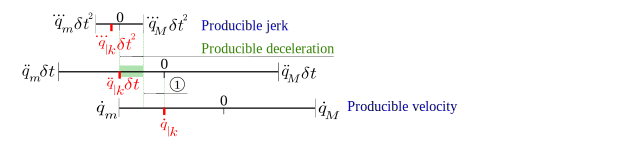
\includegraphics[width=1.0\columnwidth]{/home/anis/Desktop/THESIS_ANIS/THESIS/figures/Constrcomp/Constraints_incompatibility4_JR}
\caption{Extended state {\color{red} $S_{|k}$} of an articular joint moving towards its lower position limit $\vect{q}_m$ and one time-step before reaching its velocity limit $\vect{\dot{q}}_{m}$. The producible jerk is limiting the range from which the control variable $\vect{\ddot{q}}_{|k}^{c}$ can be picked: $\vect{\ddot{q}}_{|k}^{c}$ cannot be chosen equal to zero. Therefore, at the next time-step, at which $\vect{\dot{q}}_{|k}$ is equal to $\vect{\dot{q}}_{m}$, the articular acceleration cannot be brought to zero. The joint will continue to accelerate and the velocity limit will inevitably be violated. Because of the incompatibility with the producible jerk, it is impossible in this case to cope with the constraint on articular velocity. The incompatibility disappears if an actuator that can produce a larger amount of jerk is used: gape \circled{1} disappears.}
\label{fig:Constraints_incompatibility_vel_constr_JR}
\end{figure*}
\item \textbf{Incompatibility cases related to the joint position constraint:}
On the other hand, coping with a joint position constraint implies bringing both the articular velocity $\vect{\dot{q}}_{|k}$ and acceleration $\vect{\ddot{q}}_{|k}$ to zero when hitting the max/min position boundaries $[\vect{q}_{M}, \vect{q}_{m}]$. In this case, two incompatibility cases may arise: 
\begin{enumerate}[label=\Alph*]
\item \underline{The first} is when no sufficient articular deceleration is available during the implicitly induced braking phase (that lasts $1$ control time-step) even if sufficient braking jerk can be produced (see Fig.~\ref{fig:Constraints_incompatibility_posi_constr1}). 
\item \underline{The second} is when no sufficient jerk capabilities are available even if enough deceleration can be generated by the considered actuator (see Fig.~\ref{fig:Constraints_incompatibility_posi_constr2}).
\end{enumerate}
\begin{figure*}
\centering
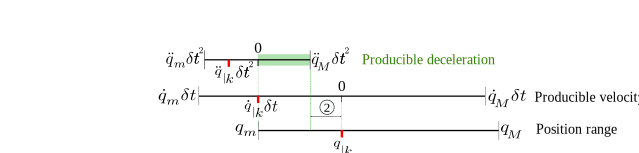
\includegraphics[width=1.0\columnwidth]{/home/anis/Desktop/THESIS_ANIS/THESIS/figures/Constrcomp/Constraints_incompatibility4_PC1}
\caption{Extended state {\color{red} $S_{|k}$} of an articular joint moving towards and one time-step before reaching its lower position limit $q_{m}$. The range of producible deceleration $\ddot{q}_{|k}^{c}$ is not sufficient to allow forcing the articular velocity to zero at the next time-step, at which $q_{|k}$ becomes equal to $q_m$. Because of the incompatibility with the deceleration capability, it is impossible in this case to satisfy the joint position constraint. This incompatibility disappears if an actuator that can produce a larger amount of  deceleration is used: gape \circled{2} disappears.}
\label{fig:Constraints_incompatibility_posi_constr1}
\end{figure*}
\begin{figure*}
\centering
\includegraphics[width=1.0\columnwidth]{/home/anis/Desktop/THESIS_ANIS/THESIS/figures/Constrcomp/Constraints_incompatibility4_PC2}
\caption{Extended state {\color{red} $S_{|k}$} of an articular joint moving towards and one time-step before reaching its lower position limit $q_{m}$. The producible jerk is limiting the range from which the control variable $\ddot{q}_{|k}^{c}$ can be picked: $\ddot{q}_{|k}^{c}$ cannot be chosen equal to zero. Therefore, it is not possible to force the articular velocity to zero for the next time-step, at which $q_{|k}$ becomes equal to $q_m$. Because of the incompatibility with the producible jerk, it is impossible in this case to cope with the joint position constraint. The incompatibility disappears if an actuator that can produce a larger amount of jerk is used: gape \circled{3} disappears.}
\label{fig:Constraints_incompatibility_posi_constr2}
\end{figure*}
\end{enumerate}
%%%%%%%%%%%%%%%%%%%%%%%%%%SUBSUBSECTION%%%%%%%%%%%%%%%%%%%%%%%%%%%%%
%%%%%%%%%%%%%%%%%%%%%%%%%%SUBSUBSECTION%%%%%%%%%%%%%%%%%%%%%%%%%%%%%
%\subsubsection{Incompatibility case related to the constraint on articular velocity}
%\label{subsubsec:inc_jnt_cnstr}
%Coping with a joint velocity constraint automatically implies bringing the articular acceleration $\vect{\ddot{q}}_{|k}$ to zero when hitting a Max/min velocity limit $[\vect{\dot{q}}_{m}, \vect{\dot{q}}_{M}]$. In such case, an incompatibility problem may arise if no sufficient articular jerk can be produced by the actuator of the robot during the implicitly induced braking phase that brings the articular acceleration to zero. Coping at the same time with the articular velocity limit and the articular jerk limit may become impossible (see Fig.~\ref{fig:Constraints_incompatibility_vel_constr_JR}).
%\begin{figure*}
%\centering
%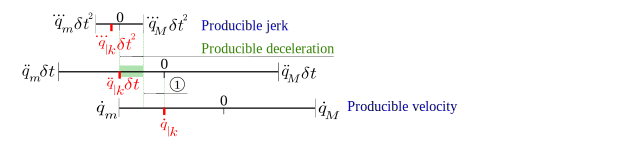
\includegraphics[width=1.0\columnwidth]{/home/anis/Desktop/THESIS_ANIS/THESIS/figures/Constrcomp/Constraints_incompatibility4_JR}
%\caption{Extended state {\color{red} $S_{|k}$} of an articular joint moving towards its lower position limit $\vect{q}_m$ and one time-step before reaching its velocity limit $\vect{\dot{q}}_{m}$. The producible jerk is limiting the range from which the control variable $\vect{\ddot{q}}_{|k}^{c}$ can be picked: $\vect{\ddot{q}}_{|k}^{c}$ cannot be chosen equal to zero. Therefore, at the next time-step, at which $\vect{\dot{q}}_{|k}$ is equal to $\vect{\dot{q}}_{m}$, the articular acceleration cannot be brought to zero. The joint will continue to accelerate and the velocity limit will inevitably be violated. Because of the incompatibility with the producible jerk, it is impossible in this case to cope with the constraint on articular velocity. The incompatibility disappears if an actuator that can produce a larger amount of jerk is used: gape \circled{1} disappears.}
%\label{fig:Constraints_incompatibility_vel_constr_JR}
%\end{figure*}
%%%%%%%%%%%%%%%%%%%%%%%%%%%SUBSUBSECTION%%%%%%%%%%%%%%%%%%%%%%%%%%%%%
%%%%%%%%%%%%%%%%%%%%%%%%%%%SUBSUBSECTION%%%%%%%%%%%%%%%%%%%%%%%%%%%%%
%\subsubsection{Incompatibility cases related to the joint position constraint}
%On the other hand, coping with a joint position constraint implies bringing both the articular velocity $\vect{\dot{q}}_{|k}$ and acceleration $\vect{\ddot{q}}_{|k}$ to zero when hitting the Max/min position boundaries $[\vect{q}_{M}, \vect{q}_{m}]$. In this case, two incompatibility cases may arise. The first is when no sufficient articular deceleration is available during the implicitly induced braking phase (that lasts $1$ control time-step) even if sufficient braking jerk can be produced (see Fig.~\ref{fig:Constraints_incompatibility_posi_constr1}). The second is when no sufficient jerk capabilities are available even if enough deceleration can be generated by the considered actuator (see Fig.~\ref{fig:Constraints_incompatibility_posi_constr2}).
%\begin{figure*}
%\centering
%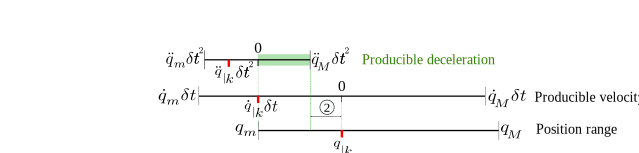
\includegraphics[width=1.0\columnwidth]{/home/anis/Desktop/THESIS_ANIS/THESIS/figures/Constrcomp/Constraints_incompatibility4_PC1}
%\caption{Extended state {\color{red} $S_{|k}$} of an articular joint moving towards and one time-step before reaching its lower position limit $q_{m}$. The range of producible deceleration $\ddot{q}_{|k}^{c}$ is not sufficient to allow forcing the articular velocity to zero at the next time-step, at which $q_{|k}$ becomes equal to $q_m$. Because of the incompatibility with the deceleration capability, it is impossible in this case to satisfy the joint position constraint. This incompatibility disappears if an actuator that can produce a larger amount of  deceleration is used: gape \circled{2} disappears.}
%\label{fig:Constraints_incompatibility_posi_constr1}
%\end{figure*}
%\begin{figure*}
%\centering
%\includegraphics[width=1.0\columnwidth]{/home/anis/Desktop/THESIS_ANIS/THESIS/figures/Constrcomp/Constraints_incompatibility4_PC2}
%\caption{Extended state {\color{red} $S_{|k}$} of an articular joint moving towards and one time-step before reaching its lower position limit $q_{m}$. The producible jerk is limiting the range from which the control variable $\ddot{q}_{|k}^{c}$ can be picked: $\ddot{q}_{|k}^{c}$ cannot be chosen equal to zero. Therefore, it is not possible to force the articular velocity to zero for the next time-step, at which $q_{|k}$ becomes equal to $q_m$. Because of the incompatibility with the producible jerk, it is impossible in this case to cope with the joint position constraint. The incompatibility disappears if an actuator that can produce a larger amount of jerk is used: gape \circled{3} disappears.}
%\label{fig:Constraints_incompatibility_posi_constr2}
%\end{figure*}
%%%%%%%%%%%%%%%%%%%%%%%%%%SUBSECTION%%%%%%%%%%%%%%%%%%%%%%%%%%%%%
%%%%%%%%%%%%%%%%%%%%%%%%%%%%%%%%%%%%%%%%%%%%%%%%%%%%%%%%%%%%%%%%%
%%%%%%%%%%%%%%%%%%%%%%%%%%SUBSECTION%%%%%%%%%%%%%%%%%%%%%%%%%%%%%
\section{Test case scenario for simulation}
In this section, the test case scenario used as a basis for testing all the different formulations of the constraints on articular velocity and position is presented. A comparison between the naive and new formulations will then be performed in Section~\ref{sec:art_cnstr_new_frml}. The controller described in Section~\ref{subsec:cntrl_frm} is implemented as a C++ Orocos component \cite{rtt-url} on a virtual model of the KUKA LWR4 serial robot using XDE, a robotics-oriented physics simulation engine \cite{merlhiot2012}. 

As a main activity, the robot performs a trajectory tracking task where its joints track desired articular positions \textit{(discovered at every time-step)} (see Fig.~\ref{fig:kuka_screen}). During its movement, the system is pushed to its physical limits (max/min articular positions, velocities, accelerations and jerks). The LQP is solved in real-time at a period of $1~ms$ using Gurobi, a commercial optimization software \cite{gurobi}. Values used for the gains of the controller during simulation are: $K_p=400$, $K_d=2\sqrt{K_p}$. $Q_t$ and $Q_r$ in this case are identity matrices. For demonstration purposes, only the physical capabilities of the first joint of the robot (joint $0$) are constrained. 
%As a main activity, the robot performs a trajectory tracking task where the end-effector tracks a desired position and orientation \textit{(discovered at every time-step)} in Cartesian space (see Fig.~\ref{fig:kuka_screen}). During its movement, the system is pushed to its physical limits (articular positions, velocities, accelerations and jerks). The LQP is solved in real time at a period of 1\textit{ms} using Gurobi, a commercial optimization software \cite{gurobi}. For demonstration purposes, only the physical capabilities of the first joint of the robot will be constrained. 
%The articular limitations are chosen as following: 
%$[q_{0_{m}}, q_{0_{M}}]=[,]$, $[\dot{q}_{0_{m}}, \dot{q}_{0_{M}}]=[,]$, $[\ddot{q}_{0_{m}}, \ddot{q}_{0_{M}}]=[,]$, $[\dddot{q}_{0_{m}}, \dddot{q}_{0_{M}}]=[,]$.  
\begin{figure}[!htbp]
\centering
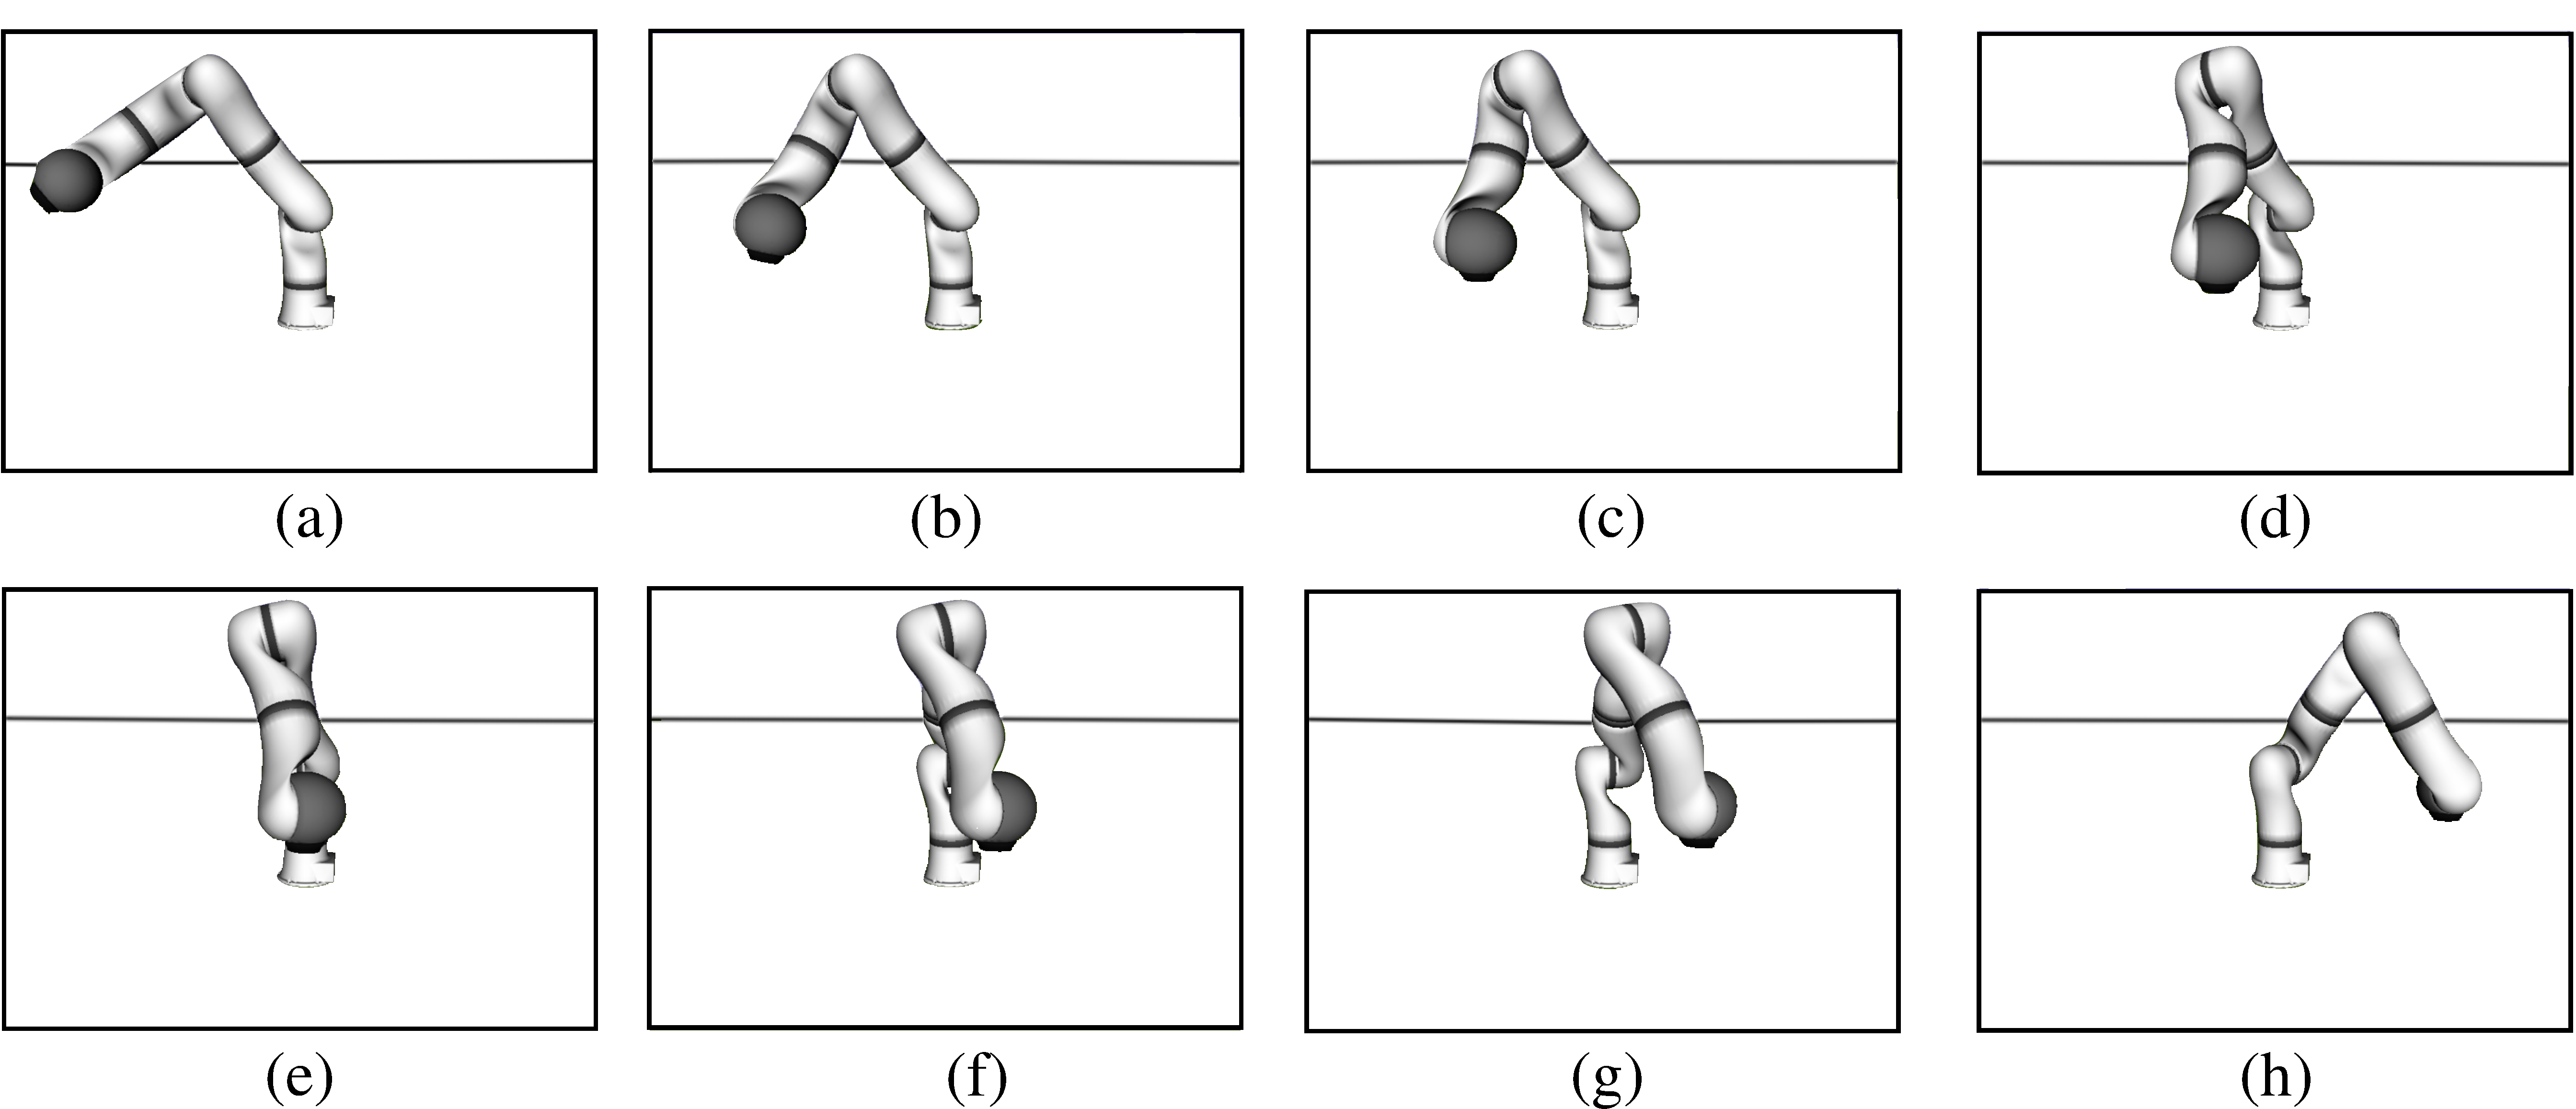
\includegraphics[width=1.0\columnwidth]{/home/anis/Desktop/THESIS_ANIS/THESIS/figures/Constrcomp/kuka_screen}
\caption{Screenshots of the test case scenario simulation with the KUKA LWR4 robot.}
\label{fig:kuka_screen}
\end{figure*}
\begin{figure}[!htbp]
\centering
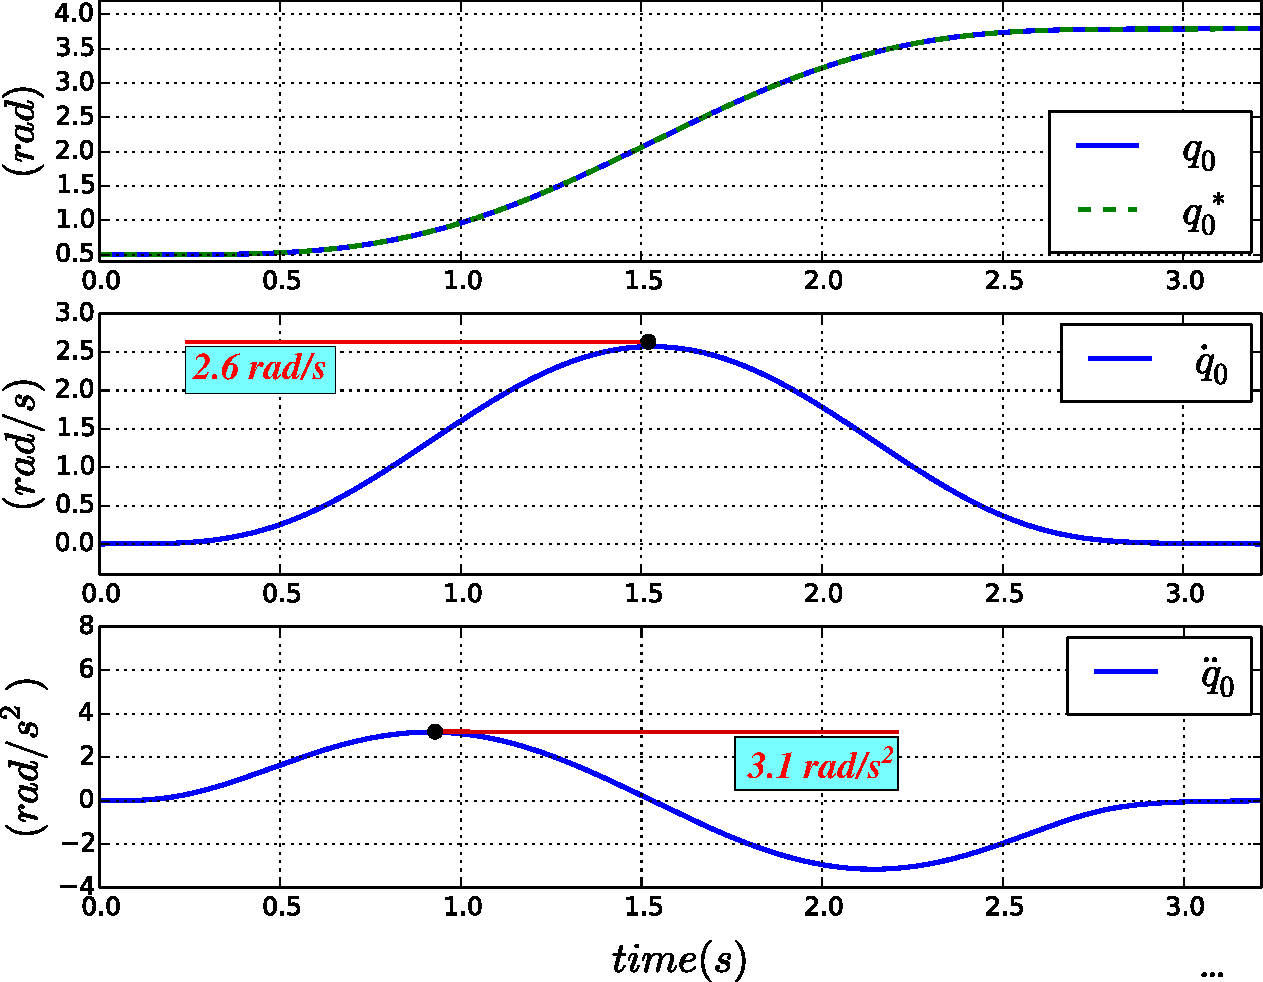
\includegraphics[width=0.8\columnwidth]{/home/anis/Desktop/THESIS_ANIS/THESIS/figures/Constrcomp/No_constr_move}
\caption{Extended state $S$ of joint $0$ during the test case scenario. The movement of the joint is not constrained. Top to bottom: position, velocity, acceleration and jerk.}
\label{fig:No_constr_move}
\end{figure}
\\
Fig.~\ref{fig:No_constr_move} shows the extended state of joint $0$ as it reaches its desired position $q_0^*=3.79~rad$\footnote{The position range for joint $0$ on a real KUKA LWR4 is $[q_{m_{0}}, q_{M_{0}}]=[-2.97, 2.97]~rad$. A wider domain is considered in simulation.} within $3.5~s$. During its movement, joint $0$ reaches a maximum velocity of $2.57~rad.s^{-1}$, a maximum acceleration of $3.15~rad.s^{-2}$ and a maximum jerk of $-8.05~rad.s^{-3}$.
%%%%%%%%%%%%%%%%%%%%%%%%%%%%%%%%%%%%%%%%%%%%%%%%%%%%%%%%%
       %Articular constraints: new formulations%
%%%%%%%%%%%%%%%%%%%%%%%%%%%%%%%%%%%%%%%%%%%%%%%%%%%%%%%%%                         
\section{Articular constraints: new formulations}
\label{sec:art_cnstr_new_frml}
In this section, the incompatibility cases previously exposed for the articular velocity and position constraints are resolved. The classic (naive) formulation of the articular velocity constraint is modified to include the actuators jerk capabilities. The naive expression of the joint position constraint on the other hand, is  reformulated to take into account both the amounts of deceleration and jerk producible by the actuators of the robot. Considering these reaction capabilities and compared to the cases where the naive formulations of the constraints are used, the braking phases \textit{implicitly induced} on the movements of a constrained articulation start earlier, and at the right time to cope with the different joint's physical limitations. Each incompatibility case is resolved as follows: first, the extended state $S$ of the joint during the \textit{implicitly induced} braking phase\footnote{Induced at the activation of the constraint.} is described then second, based on this description, the new formulations of the constraints on articular velocity and position are derived. Finally, the behaviour of the robot with the new formulations of the constraints is compared to its behaviour when the naive ones are used. 
%%%%%%%%%%%%%%%%%%%%%%%%%%SUBSECTION%%%%%%%%%%%%%%%%%%%%%%%%%%%%%
%%%%%%%%%%%%%%%%%%%%%%%%%%%%%%%%%%%%%%%%%%%%%%%%%%%%%%%%%%%%%%%%%
%%%%%%%%%%%%%%%%%%%%%%%%%%SUBSECTION%%%%%%%%%%%%%%%%%%%%%%%%%%%%%
\subsection{Joint velocity constraint incompatibility with jerk limits}
\label{subsec:jnt_vel_cnstr_inc_jerk}
As previously explained, the constraint on the articular velocity of the robot (\ref{eq:cnt_lit_tme_step_2}) and the one on its producible articular jerk (\ref{eq:cnt_lit_tme_step_4})
may become incompatible if a joint gets close to one of its velocity limits too fast (see Fig.~\ref{fig:Constraints_incompatibility_vel_constr_JR}). In  this case, admissible\footnote{Regarding either the dynamic capabilities of the actuator or the task to be performed by the robot.} jerk may not be sufficient to allow a quick variation of the articular torque and it becomes impossible to bring the articular acceleration to zero within only one control time-step. The only solution to preserve compatibility is to \textit{induce an implicit} braking phase with maximum jerk, several time-steps (not just one) before reaching the velocity boundary. The braking phase lasts therefore $(n_{1} \in \mathbb{N}\geq 1)$ control time-steps. 
\\
Lets consider the braking phase for a joint moving towards and reaching its maximum velocity limit $\dot{q}_{M}$. During this phase, the actuator brakes with constant jerk $\dddot{q}_{m} \leq 0$ until maximum velocity $\dot{q}_{M} \geq 0$ is attained. The extended state \textit{S} of the system during such phase can be described (Note that the upcoming calculations are performed for each joint of the robot. $q$, $\dot{q}$, $\ddot{q}$, $\dddot{q}$ respectively represent one of the components of $\vect{q}}$, $\vect{\dot{q}}$, $\vect{\ddot{q}}$, $\vect{\dddot{q}}$ (in bold)):
\begin{equation} 
\begin{split}
\textit{S}_{|k+1}&\left\{\begin{array}{lcl}
\dot{q}_{|k+1} \hspace{1mm}= \dot{q}_{|k} + \ddot{q}_{|k} \delta t, \\
\ddot{q}_{|k+1} \hspace{1mm}= \ddot{q}_{|k} + \dddot{q}_{m} \delta t;
\end{array}\right.\\
\textit{S}_{|k+2}&\left\{\begin{array}{lcl}
\dot{q}_{|k+2} \hspace{1mm}= \dot{q}_{|k+1} + \ddot{q}_{|k+1} \delta t, \\
\ddot{q}_{|k+2} \hspace{1mm}= \ddot{q}_{|k+1} + \dddot{q}_{m} \delta t;
\end{array}\right.\\
& \hspace{7mm}\vdots\ \hspace{12mm}\vdots\\\
\textit{S}_{|k+n_{1}}&\left\{\begin{array}{lcl}
\dot{q}_{|k+n_{1}} = \dot{q}_{|k+n_{1}-1} + \ddot{q}_{|k+n_{1}-1} \delta t, \\
%\vspace{2mm}
\ddot{q}_{|k+n_{1}} = \ddot{q}_{|k+n_{1}-1} + \dddot{q}_{m} \delta t.
\end{array}\right.
\end{split}
\label{eq:discretized_dynamics_vel}
\end{equation}
With: $\dot{q}_{|k} \geq 0$, $\ddot{q}_{|k} \geq 0$ and  $\dddot{q}_{m} \leq 0$. The joint velocity evolution in $n_1$ iterations is equal to the general form\footnote{Computed using Maple \cite{maple}.} of the numerical sequence (\ref{eq:discretized_dynamics_vel}):
\begin{equation}
\begin{split}
\dot{q}_{|k+n_1} = \dot{q}_{|k} + n_1 \ddot{q}_{|k} \delta t + \frac{(n_1^2-n_1)}{2} \dddot{q}_{m} \delta t^2.
\label{eq:q_dot_evolution_with_const_qdddot_m}
\end{split}
\end{equation}
In case of a control at the dynamic-level, considering (\ref{eq:cmd_input_dyn}), the condition $\dot{q}_{|k+n_1} \leq \dot{q}_{M}$ for all integer $n_1$ leads to:
\begin{equation}
\begin{split}
\ddot{q}_{|k}^{c} \leq \frac{(\dot{q}_M-\dot{q}_{|k})}{n_1 \delta t} - \frac{(n_1-1)}{2} \dddot{q}_m \delta t. 
\label{eq:q_ddot_vel_jerk_comp_aa_n1}
\end{split}
\end{equation}
With $n_1$, the integer minimizing the right-hand side of (\ref{eq:q_ddot_vel_jerk_comp_aa_n1}). By differentiating this expression w.r.t $n_1$:
\begin{equation} 
\hspace{-4mm}
\left. \begin{array}{r} 
n_1 \geq 1 \\
\myfrac[5pt]{-(\dot{q}_M-\dot{q}_{|k})}{n_1^2 \delta t} - \frac{\delta t}{2} \dddot{q}_m  = 0
\end{array} \right\} 
\Rightarrow n_1=-\myfrac[5pt]{\sqrt{-2\dddot{q}_m(\dot{q}_M-\dot{q}_{|k})}}{\dddot{q}_m \delta t}.
\label{eq:n_1_eq_aa}
\end{equation}
Following the same reasoning for the lower velocity limit, the condition $\dot{q}_{|k+n_2} \geq \dot{q}_{m}$ for all integer $n_2 \geq 1$ becomes: 
\begin{equation}
\begin{split}
\ddot{q}_{|k}^{c} \geq \frac{(\dot{q}_m-\dot{q}_{|k})}{n_2 \delta t} - \frac{(n_2-1)}{2} \dddot{q}_M \delta t.
\label{eq:q_ddot_vel_jerk_comp_aa_n2}
\end{split}
\end{equation}
With:
\begin{equation}
n_2 = \myfrac[5pt]{\sqrt{-2\dddot{q}_M(\dot{q}_m-\dot{q}_{|k})}}{\dddot{q}_M \delta t}, 
\label{eq:n_2_eq_aa}
\end{equation}
maximizing the right-hand side of (\ref{eq:q_ddot_vel_jerk_comp_aa_n2}). \\
$n_1$ is the number of time-steps corresponding to the span of a braking phase implicitly induced by an articulation moving towards its upper velocity limit $\dot{q}_{M}$, and during which its positive acceleration is brought to zero by jerking negatively with $\dddot{q}_m$; and $n_1$ is the number of time-steps corresponding to the span of a braking phase implicitly induced by an articulation moving towards its lower velocity limit $\dot{q}_{m}$, and during which its negative acceleration is brought to zero by jerking positively using $\dddot{q}_M$.\\
Finally, the reflected constraint on the acceleration control variable $\ddot{q}_{|k}^{c}$ is of the form: 
\begin{equation}
\begin{split}
f_{\beta}(\dot{q}_{|k}, \dot{q}_m, \dddot{q}_M, n_2) \leq \ddot{q}_{|k}^{c} \leq f_{\alpha}(\dot{q}_{|k}, \dot{q}_M, \dddot{q}_m, n_1), 
\label{eq:qddot_cond_to_satisfy_Jerk_Vel_compatibility_profile}
\end{split}
\end{equation}
with $f_{\beta}$ and $f_{\alpha}$ as in (\ref{eq:q_ddot_vel_jerk_comp_aa_n1}) and (\ref{eq:q_ddot_vel_jerk_comp_aa_n2}).
%********************************************************************%
\subsubsection{Illustration 1}
To illustrate this first theoretical result, in this simulation, using the test case scenario, joint $0$ moves towards its upper velocity limit $\dot{q}_{M_{0}}$. Only the classic (naive) formulation of the joint velocity constraint (\ref{eq:cnt_lit_tme_step_2}) is implemented with the controller: (\ref{eq:ctrl_pb}), (\ref{eq:dyn_eq}). The constraint on articular jerk (\ref{eq:cnt_lit_tme_step_4}) is not considered. 
%0
\begin{figure}[!htbp]
\centering
{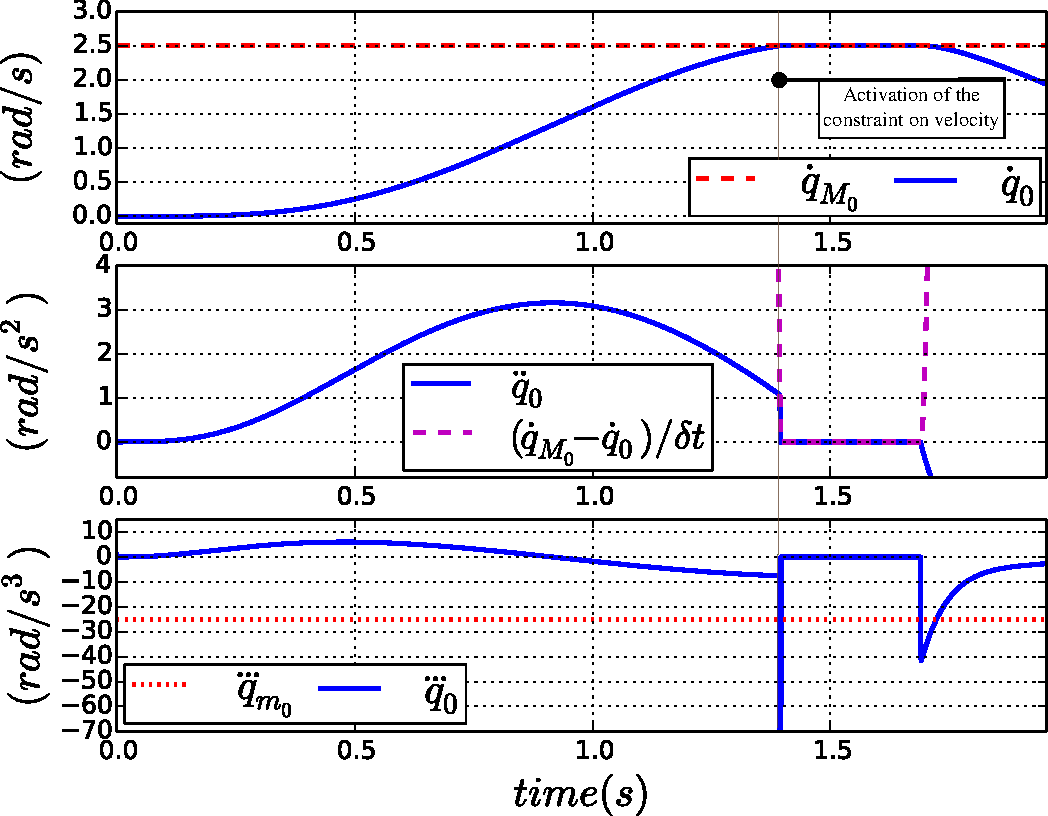
\includegraphics[width=0.8\columnwidth]{/home/anis/Desktop/THESIS_ANIS/THESIS/figures/Constrcomp/0_Vel_constr_classic}}
\caption{Extended state $S$ of joint $0$ during the braking phase (that lasts 1 control time-step $= 1~ms$) implicitly induced to cope with the maximum velocity limit $\dot{q}_{M_{0}}$. The naive formulation of the articular velocity constraint (\ref{eq:cnt_lit_tme_step_2}) is used. Top to bottom: velocity, acceleration and jerk.} 
\label{fig:0_Vel_constr_classic}
\end{figure}
Fig.~\ref{fig:0_Vel_constr_classic} shows the extended state of joint $0$ during a braking phase implicitly induced only one control time-step ($1~ms$) before reaching $\dot{q}_{M_{0}}$. A high peak of jerk is induced. In this case, if the constraint on articular jerk (\ref{eq:cnt_lit_tme_step_4}) is implemented in the controller's configuration, the control problem becomes impossible to solve. It is then clear that for a real system with limited jerk capabilities $($e.g., $\dddot{q}_{M_{0}} = 25~rad.s^{-3})$, coping with a velocity limit using the naive formulation of the articular velocity constraint is simply impossible. \\
On the other hand, when the new formulation of this constraint (\ref{eq:q_ddot_vel_jerk_comp_aa_n1}) is used, the system starts braking $n_1$ time-steps before reaching the velocity limit $\dot{q}_{M_0}$ (see Fig.~\ref{fig:1_Vel_constr_jerk_comp}). Joint $0$ is capable of coping at the same time with both its velocity and jerk limits (see Fig.~\ref{fig:1_Vel_constr_jerk_comp_zoom}). In this case, including the constraint on articular jerk (\ref{eq:cnt_lit_tme_step_4}) in the configuration of the controller will not result into an infeasible control problem. Therefore, the incompatibility between the articular velocity and jerk constraints is resolved.
%1
\begin{figure}[!htbp]
\centering
{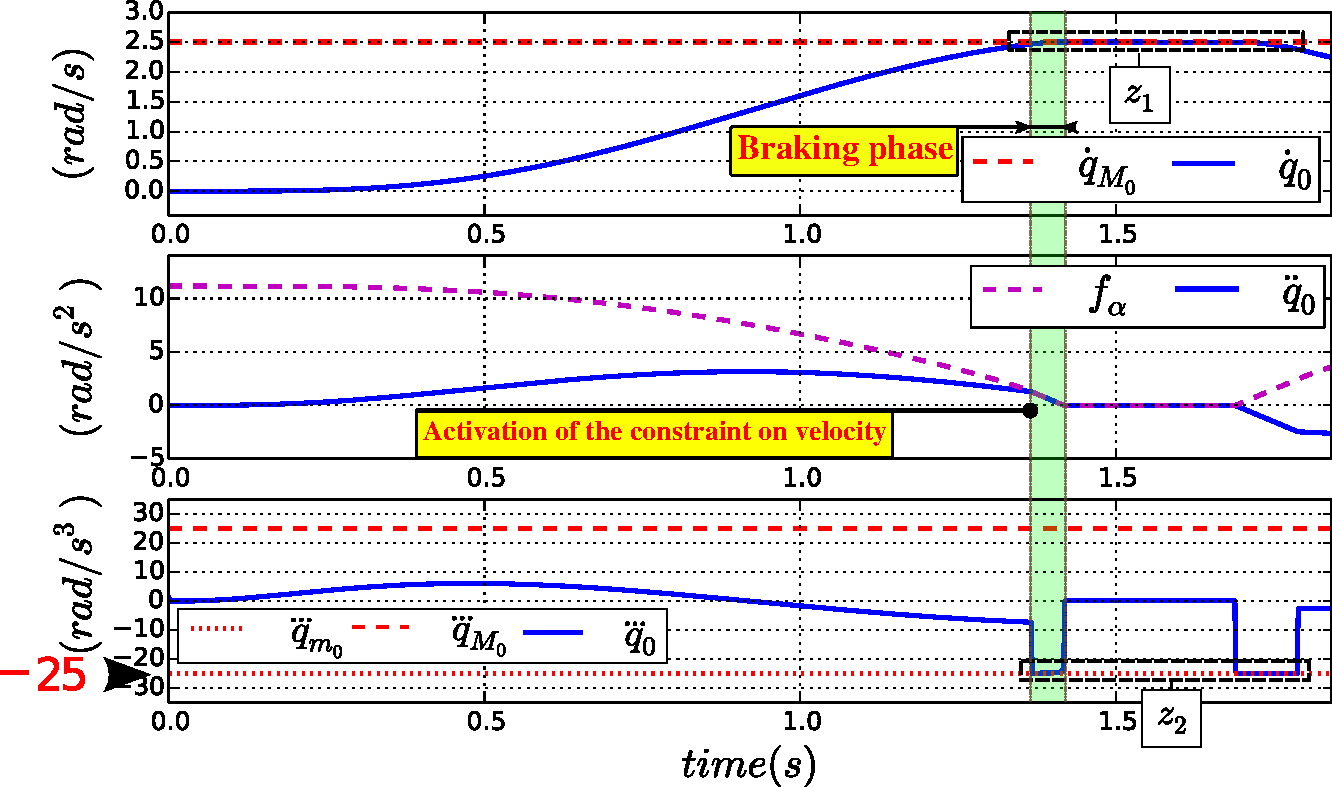
\includegraphics[width=0.9\columnwidth]{/home/anis/Desktop/THESIS_ANIS/THESIS/figures/Constrcomp/1_Vel_constr_jerk_comp_}}
\caption{Extended state $S$ of joint $0$ during the braking phase implicitly induced to cope with a maximum velocity limit $\dot{q}_{M_{0}}$. In this case, the new formulation of the constraint on articular velocity (\ref{eq:q_ddot_vel_jerk_comp_aa_n1}) that takes into account the actuator's maximum producible jerk $(\dddot{q}_{m_{0}} = 25~rad.s^{-3})$ is used. Note that $n_1$, is physically meaningful only during the span of the implicitly induced braking phase. Top to bottom: velocity, acceleration, jerk and $n_1$. $z_1$ and $z_2$ are in Fig.~\ref{fig:1_Vel_constr_jerk_comp_zoom}}. 
\label{fig:1_Vel_constr_jerk_comp}
\end{figure}
\begin{figure}[!htbp]
\centering
{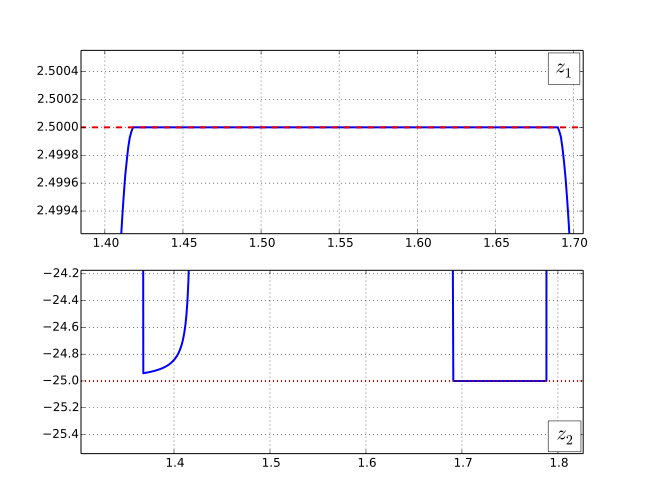
\includegraphics[width=0.8\columnwidth]{/home/anis/Desktop/THESIS_ANIS/THESIS/figures/Constrcomp/1_Vel_constr_jerk_comp_zoom}}
\caption{Zooms corresponding to Fig.~\ref{fig:1_Vel_constr_jerk_comp}.} 
\label{fig:1_Vel_constr_jerk_comp_zoom}
\end{figure}
%
%\begin{landscape}
%\begin{figure}
%\begin{minipage}[c]{0.48\linewidth}
%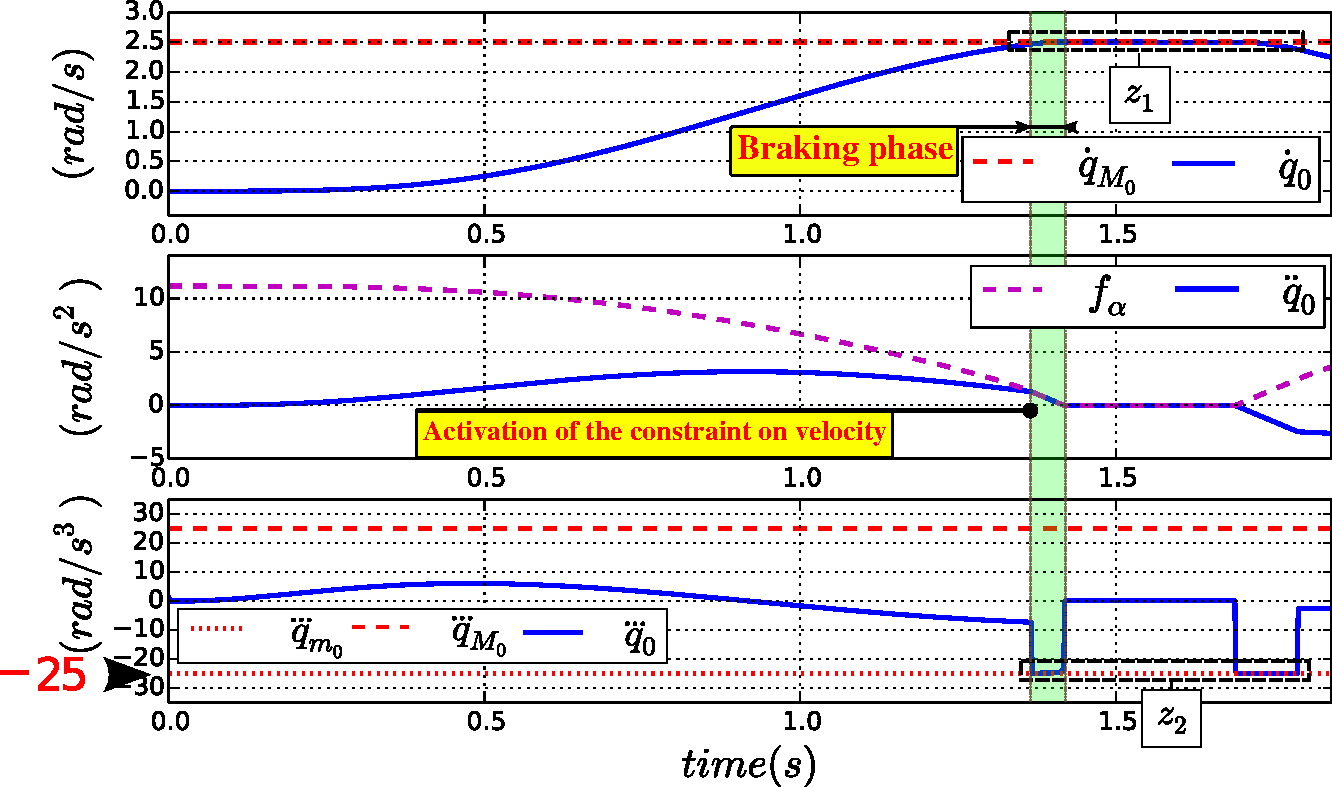
\includegraphics[width=0.99\columnwidth]{/home/anis/Desktop/THESIS_ANIS/THESIS/figures/Constrcomp/1_Vel_constr_jerk_comp_}
%\caption{State $S$ of joint $0$ during the braking phase to cope with a maximum velocity limit. In this test, the new constraint formulation (\ref{eq:q_ddot_vel_jerk_comp_aa_n1}) that takes into account the jerk capability $\dddot{q}_{M_{0}} = 25~rad.s^{-3}$ is used. Top to bottom: velocity, acceleration, jerk and $n_1$} 
%\label{fig:1_Vel_constr_jerk_comp_}
%\end{minipage}
%\hfill
%\begin{minipage}[c]{0.48\linewidth}
%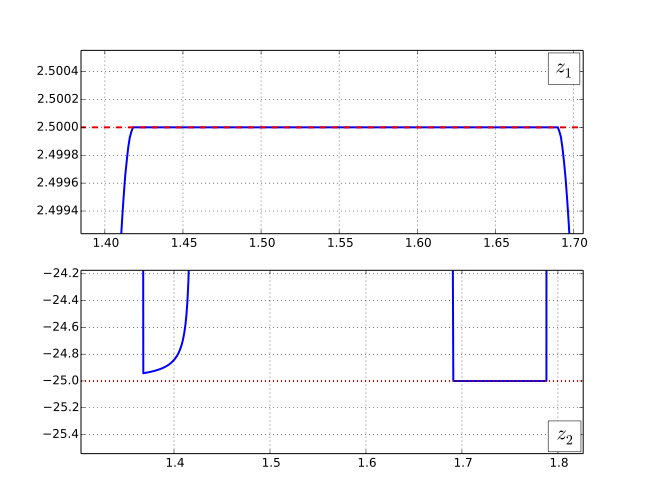
\includegraphics[width=0.99\columnwidth]{/home/anis/Desktop/THESIS_ANIS/THESIS/figures/Constrcomp/1_Vel_constr_jerk_comp_zoom}
%\caption{Zooms corresponding to Fig.~\ref{fig:1_Vel_constr_jerk_comp_}.} 
%\label{fig:1_Vel_constr_jerk_comp_zoom}
%\end{minipage}%
%\end{figure}
%\end{landscape}
%
%\begin{landscape}
%\begin{figure}
%\begin{minipage}[c]{0.48\linewidth}
%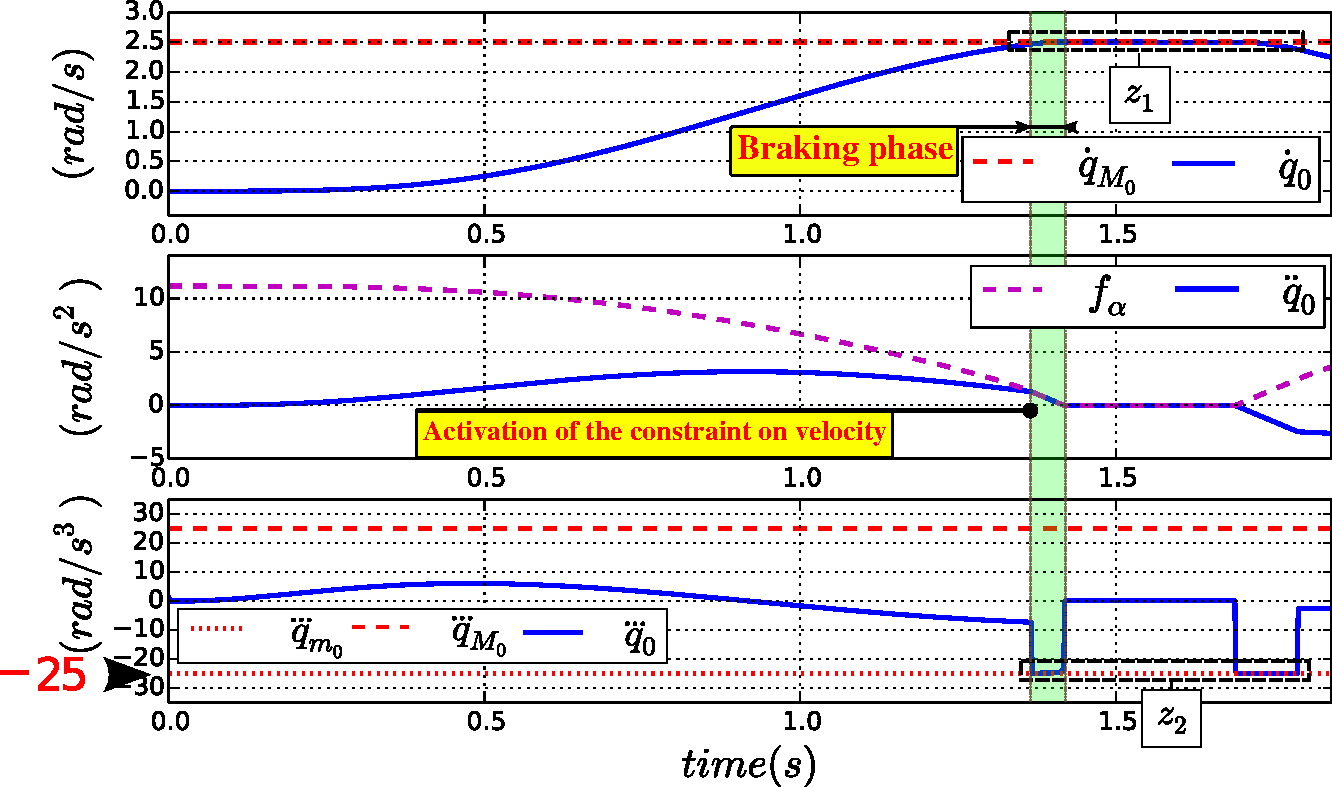
\includegraphics[width=0.99\columnwidth]{/home/anis/Desktop/THESIS_ANIS/THESIS/figures/Constrcomp/1_Vel_constr_jerk_comp_}
%\caption{State $S$ of joint $0$ during the braking phase to cope with a maximum velocity limit. In this test, the new constraint formulation (\ref{eq:q_ddot_vel_jerk_comp_aa_n1}) that takes into account the jerk capability $\dddot{q}_{M_{0}} = 25~rad.s^{-3}$ is used. Top to bottom: velocity, acceleration, jerk and $n_1$} 
%\label{fig:1_Vel_constr_jerk_comp_}
%\end{minipage}
%\hfill
%\begin{minipage}[c]{0.48\linewidth}
%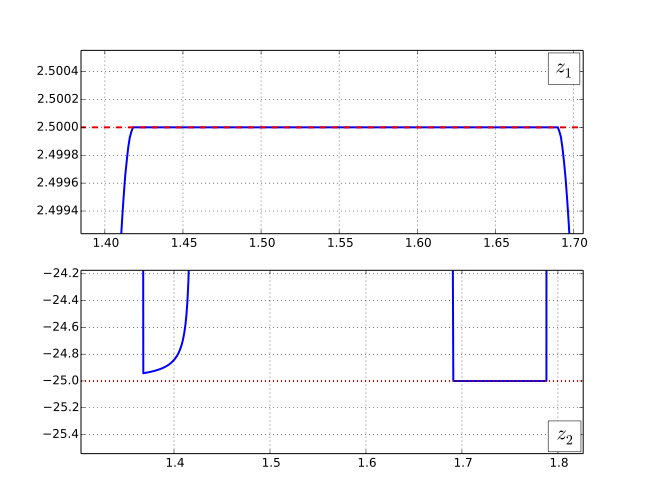
\includegraphics[width=0.99\columnwidth]{/home/anis/Desktop/THESIS_ANIS/THESIS/figures/Constrcomp/1_Vel_constr_jerk_comp_zoom}
%\caption{Zooms corresponding to Fig.~\ref{fig:1_Vel_constr_jerk_comp_}.} 
%\label{fig:1_Vel_constr_jerk_comp_zoom}
%\end{minipage}%
%\end{figure}
%\end{landscape}
%%%%%%%%%%%%%%%%%%%%%%%%%%SUBSECTION%%%%%%%%%%%%%%%%%%%%%%%%%%%%%
%%%%%%%%%%%%%%%%%%%%%%%%%%%%%%%%%%%%%%%%%%%%%%%%%%%%%%%%%%%%%%%%%
%%%%%%%%%%%%%%%%%%%%%%%%%%SUBSECTION%%%%%%%%%%%%%%%%%%%%%%%%%%%%%
\subsection{Joint position constraint incompatibility with deceleration and/or jerk limits}
\label{subsec:complete_b_ph}
With its \textit{naive}\footnote{Naive because it does not take into account the max/min amount of deceleration and jerk producible by the actuators of the robot.} formulation, the constraint on articular position (\ref{eq:cnt_lit_tme_step_1}) may become incompatible with the constraints on articular acceleration (\ref{eq:cnt_lit_tme_step_3}) and/or jerk (\ref{eq:cnt_lit_tme_step_4}) if a joint gets close to one of its position limits too fast (see Fig.~\ref{fig:Constraints_incompatibility_posi_constr1} and Fig.~\ref{fig:Constraints_incompatibility_posi_constr2}). In such case, \textit{admissible} deceleration and/or jerk may not be sufficient to allow a fast variation of the control torque, and it becomes impossible to bring both the articular acceleration and velocity to zero within only one control time-step. For example, the \labelText{{\color{red}\underline{complete}}}{label:complete} braking phase needed to be induced by an actuator to \textit{\textbf{properly}} cope with its upper position limit $q_M$ is as follows: 
\begin{enumerate}
\item at the activation of the constraint, the actuator starts jerking with maximum negative producible jerk $(\dddot{q} = \dddot{q}_m)$ (sub-phase \circled{1} in Fig.~\ref{fig:per_Pr_jerk_ala_3}). 
\item if the maximum producible deceleration $\ddot{q}_m$ is reached, braking jerk $\dddot{q}$ is brought to zero and the ``\textit{charged}'' deceleration $(\ddot{q} = \ddot{q}_m)$ is applied during several time-steps (sub-phase \circled{2} in Fig.~\ref{fig:per_Pr_jerk_ala_3}). 
\item the amount of deceleration in the joint is finally ``\textit{de-charged}'' and brought to zero by jerking positively with maximum producible jerk $(\dddot{q} = \dddot{q}_M)$ (sub-phase \circled{3} in Fig.~\ref{fig:per_Pr_jerk_ala_3}). By the end, the joint is stopped exactly at its upper position limit $q_M$. 
\end{enumerate}
\begin{figure}[!htbp]
{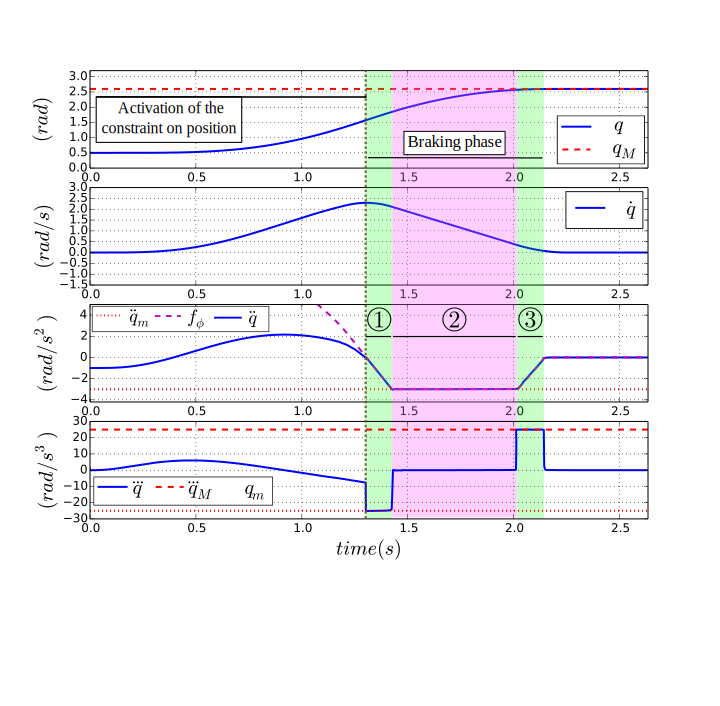
\includegraphics[width=1\columnwidth]{/home/anis/Desktop/THESIS_ANIS/THESIS/figures/Constrcomp/per_Posi_constr_jerk_acc_comp_complete_formula_3}}
\caption{Extended state $S$ of a joint during the induced \textit{complete} braking phase needed to \textit{\textbf{properly}} cope with an upper position limit $q_{M}$. The braking phase is composed of three sub-phases that each lasts for a number of time-steps: sub-phase~1 lasts $n_{15}$ control time-steps; sub-phase~2 lasts $n_{17}$ control time-steps and sub-phase~3 lasts $n_{19}$ control time-steps. Note that this illustration is not the result of a simulation. It represents the state of an actuator in case the \textit{complete} braking phase is used to cope with its upper position limit. Top to bottom: position, velocity, acceleration and jerk.} 
\label{fig:per_Pr_jerk_ala_3}
\end{figure}
As explained, coping with a joint position limit may fail because of incompatibilities with two other constraints: articular deceleration limits (\ref{eq:cnt_lit_3}) and producible articular jerk (\ref{eq:cnt_lit_4}). The resolution of these incompatibilities will be \textbf{methodically} performed as follows: 
\begin{enumerate}
\item \textbf{first}, independently from jerk capabilities, the naive expression of the position constraint (\ref{eq:cnt_lit_tme_step_1}) is modified to include solely the deceleration capabilities: $(\ddot{q}_m \leq 0)$ considering the upper position limit $(q_M \geq 0)$, and $(\ddot{q}_M  \geq 0)$ considering the lower position limit $(q_m \leq 0)$. With the new formulation, when coping for example with an upper articular position limit, the joint implicitly starts braking using its maximum deceleration capability $n_{3} \in \mathbb{N}$ iterations before reaching $q_M$ (see Fig.~\ref{fig:5_Posi_constr_acc_comp_312}). Using this formulation, both constraints on the articular position (\ref{eq:cnt_lit_1}) and the articular acceleration (\ref{eq:cnt_lit_3}) become compatible. The reflected bounds on the control variable $\ddot{q}_{|k}^{c}$ will be of the form: 
\begin{equation}
\begin{split}
f_{\xi}(q_m, \ddot{q}_M, n_4) \leq \ddot{q}_{|k}^{c} \leq f_{\gamma}(q_M, \ddot{q}_m, n_3). 
\label{eq:qddot_cond_to_satisfy_Acc_posi_compatibility}
\end{split}
\end{equation}
The proper methods to compute $n_3$, $n_4$, $f_{\gamma}$ and $f_{\xi}$ are fully defined in Section~\ref{subsec:case1}. 
\begin{figure}[!htbp]
{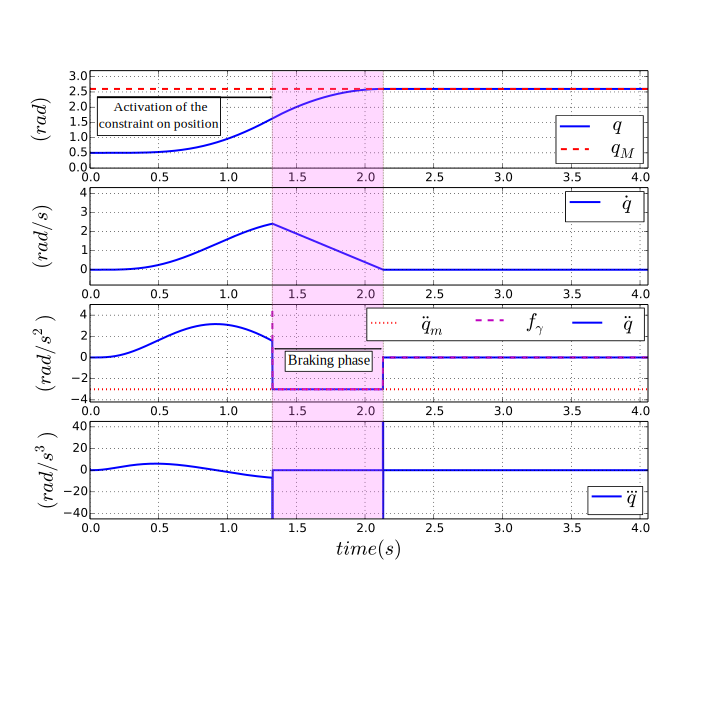
\includegraphics[width=1\columnwidth]{/home/anis/Desktop/THESIS_ANIS/THESIS/figures/Constrcomp/5_Posi_constr_acc_comp_312}}
\caption{Extended state $S$ of a joint during the induced braking phase needed to cope with an upper position limit $q_{M}$. Lasting $n_3$ control time-steps, the braking phase in this case takes into account only the articular deceleration capability $\ddot{q}_m$. Jerk limits are not considered. Top to bottom: position, velocity, acceleration and jerk.} 
\label{fig:5_Posi_constr_acc_comp_312}
\end{figure}
\item \textbf{Second}, independently from the articular deceleration capabilities, the naive expression of the constraint on articular position (\ref{eq:cnt_lit_tme_step_1}) is modified to include exclusively the actuator's jerk capabilities: $(\dddot{q}_m \leq 0)$ considering an upper position limit $(q_M \geq 0)$, and $(\dddot{q}_M \geq 0)$ when dealing with the lower position limit $(q_m \leq 0)$. With the resulting formulation, when coping for example with an upper position limit $q_M$, a braking movement is implicitly induced on the considered joint for a duration of $n_{5} \in \mathbb{N}$ control time-steps. Maximum producible negative jerk $\dddot{q}_m$ is applied by the actuator during this braking phase until the joint reaches and stops at upper position limit $q_{M}$. With such braking phase, both constraints on the articular position (\ref{eq:cnt_lit_1}) and jerk (\ref{eq:cnt_lit_3}) become compatible. In such case, the reflected bounds on the acceleration control variable will be of the form:
\begin{equation}
\begin{split}
f_{\theta}(q_m, \dddot{q}_M, n_6) \leq \ddot{q}_{|k}^{c} \leq f_{\eta}(q_M, \dddot{q}_m, n_5). 
\label{eq:qddot_cond_to_satisfy_Jerk_posi_compatibility}
\end{split}
\end{equation}
The proper methods to compute $n_5$, $n_6$, $f_{\eta}$ and $f_{\theta}$ are fully defined in Section~\ref{sec:secref2}. 
\item \textbf{Thirdly}, because of undesired oscillations (more details about this problem in subsection~\ref{sec:secref2}) that may appear in the movement of the constrained joint when using (\ref{eq:qddot_cond_to_satisfy_Jerk_posi_compatibility}) to cope with a position limit, this formulation is modified to include at the same time both the negative  $(\dddot{q}_m \leq 0)$ and positive $(\dddot{q}_M \geq 0)$ maximum producible articular jerk in both its left-hand and right-hand sides. When coping for example with an upper position limit, the  actuator should start braking with negative maximum producible jerk $\dddot{q}_m$ for $n_7$ control time-steps. As a consequence of this first braking sub-phase (phase \circled{1} in Fig.~\ref{fig:8_Podfgf12}), deceleration is ``\textit{loaded}'' in the articular joint. The actuator should then jerk positively with maximum producible jerk $\dddot{q}_M$ to bring the ``\textit{loaded}'' deceleration to zero (phase \circled{2} in Fig.~\ref{fig:8_Podfgf12}). The second sub-phase of the induced braking phase lasts for $n_9$ control time-steps and by its end, the actuator reaches and stops at its upper position limit $q_M$.  With such braking phase, the new formulation of the constraint on articular position will be of the form:
%Thirdly, because of oscillations\footnote{These oscillations are caused by not \textit{de-charging} the accumulated deceleration during the braking phase to cope with a position limit.} that may appear on the movement of the joint when using the previous formulation, (\ref{eq:qddot_cond_to_satisfy_Jerk_posi_compatibility}) will be modified to include positive and negative jerk capabilities as following:
\begin{equation}
\begin{split}
f_{\mu}(q_m, \dddot{q}_M, \dddot{q}_m, n_8, n_{10}) \leq \ddot{q}_{|k}^{c} \leq f_{\lambda}(q_M, \dddot{q}_m, \dddot{q}_M, n_7, n_9). 
\label{eq:qddot_cond_to_satisfy_Jerk_posi_compatibility_complete}
\end{split}
\end{equation}
The proper methods to compute $n_7$, $n_9$, $n_8$, $n_{10}$, $f_{\lambda}$ and $f_{\mu}$ are fully defined in Section~\ref{subsec:case3}. 
\begin{figure}[!htbp]
{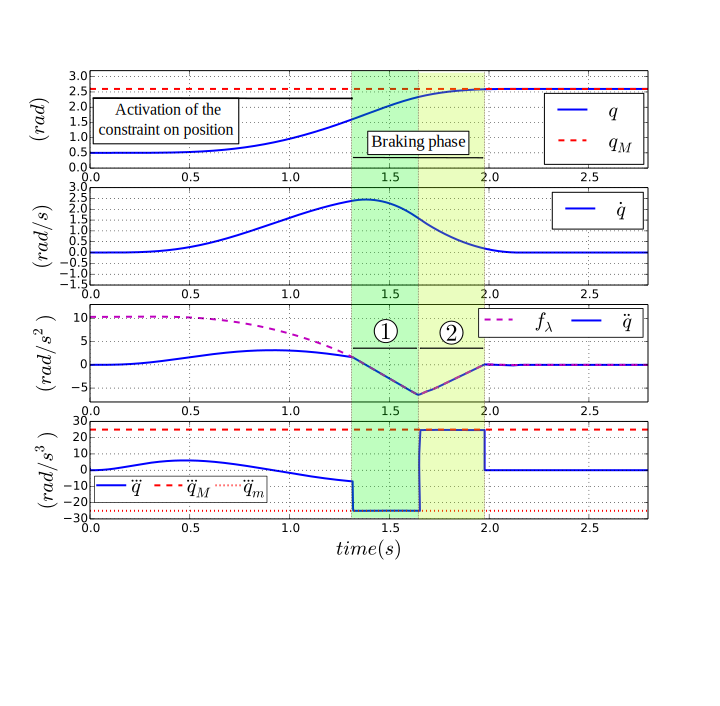
\includegraphics[width=1\columnwidth]{/home/anis/Desktop/THESIS_ANIS/THESIS/figures/Constrcomp/8_Podfgf12}}
\caption{Extended state $S$ of a joint during the induced braking phase needed to cope with an upper position limit $q_{M}$. The braking phase in this case is composed of two sub-phases: sub-phase~1 that lasts $n_{7}$ control time-steps and sub-phase~2 that lasts $n_{9}$ iterations. Note that, this illustration of the state of the joint is not the result of a simulation. It is a representation of how should be a braking phase induced using (\ref{eq:qddot_cond_to_satisfy_Jerk_posi_compatibility_complete}) when coping with an upper position limit. Top to bottom: position, velocity, acceleration and jerk.} 
\label{fig:8_Podfgf12}
\end{figure}
\item \textbf{Fourthly}, an expression of the constraint on articular position that takes into account at the same time both the jerk and deceleration capabilities is formulated. When included in the controller, this formulation renders the constraints on articular acceleration (\ref{eq:cnt_lit_3}) and jerk (\ref{eq:cnt_lit_4}) both compatible with the constraint on articular position (\ref{eq:cnt_lit_1}). Reflected bounds on the acceleration control variable $\ddot{q}_{|k}^{c}$ will be of the form: 
\begin{equation}
\begin{split}
f_{\rho}(q_m, \dddot{q}_M, \ddot{q}_M, n_{12}, n_{14}) \leq \ddot{q}_{|k}^{c} \leq f_{\pi}(q_M, \dddot{q}_m, \ddot{q}_m, n_{11}, n_{13}). 
\label{eq:qddot_cond_to_satisfy_Acc_Jerk_posi_compatibility}
\end{split}
\end{equation}
The proper methods to compute $n_{11}$, $n_{13}$, $n_{12}$, $n_{14}$, $f_{\pi}$ and $f_{\rho}$ are fully defined in Section~\ref{subsec:case4}. 
\item \textbf{Finally}, based on all the introduced forms of the various expressions proposed for the articular position constraint, a formulation that is based on the \nameref{label:complete} description of the braking phase used to \textit{\textbf{properly}} cope with a joint's upper/lower position limit is proposed. This includes the deceleration ``\textit{de-charging}'' sub-phase (sub-phase \circled{3} in Fig.~\ref{fig:per_Pr_jerk_ala_3}) that is necessary to prevent possible oscillations on the movement of the actuator during the activation of the constraint. This new and complete formulation takes into account both the negative and positive jerk capabilities $(\dddot{q}_m, \dddot{q}_M)$ together with the producible deceleration: $(\ddot{q}_m \leq 0)$ when coping with an upper position limit $(q_M \geq 0)$, and $(\ddot{q}_M \geq 0)$ when coping with a lower position limit $(q_m \leq 0)$. Without any drawbacks\footnote{No oscillations in the movement of the joint.}; both constraints on articular deceleration (\ref{eq:cnt_lit_3}) and jerk (\ref{eq:cnt_lit_4}) become compatible with the constraint on articular position (\ref{eq:cnt_lit_1}). With such formulation of the constraint on articular position derived from the \nameref{label:complete} description of the braking phase, the reflected bounds on the acceleration control variable are of the form: 
\begin{equation}
\begin{split}
f_{\chi}(q_m, \dddot{q}_M, \ddot{q}_M, \dddot{q}_m, n_{16}, n_{18}, n_{20}) \leq \ddot{q}_{|k}^{c} \leq f_{\phi}(q_M, \dddot{q}_m, \ddot{q}_m, \dddot{q}_M, n_{15}, n_{17}, n_{19}). 
\label{eq:qddot_cond_to_satisfy_Acc_Jerk_posi_compatibility2}
\end{split}
\end{equation}
The proper methods to compute $n_{15}$, $n_{17}$, $n_{19}$, $n_{16}$, $n_{18}$, $n_{20}$, $f_{\phi}$ and $f_{\chi}$ are fully defined in Section~\ref{subsec:case5}.
\end{enumerate}
\textbf{Note:} for a reactively controlled robot to optimally and \textit{properly} cope with a constraint on its articular position, considering both its max/min deceleration and jerk capabilities, the only formulation of the joint position constraint that should be implemented in its optimization control scheme is (\ref{eq:qddot_cond_to_satisfy_Acc_Jerk_posi_compatibility2}). The reader can directly check Section~\ref{subsec:case5} for the results on the behaviour of the robot when this formulation is used. The other formulations: (\ref{eq:qddot_cond_to_satisfy_Acc_posi_compatibility}), (\ref{eq:qddot_cond_to_satisfy_Jerk_posi_compatibility}), (\ref{eq:qddot_cond_to_satisfy_Jerk_posi_compatibility_complete}) and (\ref{eq:qddot_cond_to_satisfy_Acc_Jerk_posi_compatibility}), besides being presented for pedagogical reasons, their intermediary results are used for the formulation of (\ref{eq:qddot_cond_to_satisfy_Acc_Jerk_posi_compatibility2}) and taken individually, they can be used in specific cases where only the max/min producible articular deceleration OR jerk are of interest. Plus, due to the computation load linked to the $n_i$ parameters, these simpler formulations are faster to compute compared to the complete and proper formulation of the articular position constraint (\ref{eq:qddot_cond_to_satisfy_Acc_Jerk_posi_compatibility2}). \\

In the upcoming sections, the methods used to compute the introduced new formulations of the joint position constraint are furthermore detailed. In Section~\ref{sec:finalb}, the final bounds on the optimization control variable $\ddot{q}_{|k}^c$ that take into account the constraints on the articular position, velocity, acceleration and jerk all at the same time are formulated.
%%%%%%%%%%%%%%%%%%%%%%%%%%SUBSUBSECTION%%%%%%%%%%%%%%%%%%%%%%%%%%%%%
%%%%%%%%%%%%%%%%%%%%%%%%%%SUBSUBSECTION%%%%%%%%%%%%%%%%%%%%%%%%%%%%%
\subsubsection{Joint position constraint incompatibility with deceleration limits}
\label{subsec:case1}
In this section, the braking phase implicitly induced by a joint's actuator moving towards its upper position limit $q_{M}$ is considered. During this phase, the actuator's maximum producible deceleration is $\ddot{q}_{m}$. Its jerk capabilities $[\dddot{q}_{m}, \dddot{q}_{M}]$ are not considered. The extended state of the system during such braking phase, that makes the actuator stop at its position limit $q_{M}$, can be described as:
\begin{equation} 
\begin{split}
\textit{S}_{|k+1}&\left\{\begin{array}{lcl}
q_{|k+1} \hspace{1mm}= q_{|k} + \dot{q}_{|k} \delta t, \\
\dot{q}_{|k+1} \hspace{1mm}= \dot{q}_{|k} + \ddot{q}_{m} \delta t;
\end{array}\right.\\
\textit{S}_{|k+2}&\left\{\begin{array}{lcl}
q_{|k+2} \hspace{1mm}= q_{|k+1} + \dot{q}_{|k+1} \delta t, \\
\dot{q}_{|k+2} \hspace{1mm}= \dot{q}_{|k+1} + \ddot{q}_{m} \delta t;
\end{array}\right.\\
&\hspace{7mm}\vdots\ \hspace{12mm}\vdots\ \\
\textit{S}_{|k+n_{3}}&\left\{\begin{array}{lcl}
q_{|k+n_{3}} = q_{|k+n_{3}-1} + \dot{q}_{|k+n_{3}-1} \delta t, \\
\dot{q}_{|k+n_{3}} = \dot{q}_{|k+n_{3}-1} + \ddot{q}_{m} \delta t.
\end{array}\right.
\end{split}
\label{eq:discretized_dynamics_posi_decel}
\end{equation}
With: $q_{|k} \geq 0$, $\dot{q}_{|k} \geq 0$ and  $\ddot{q}_{m} \leq 0$ (braking phase). The joint position evolution in $n_3  \geq 1$ iterations is equal to the general form\footnote{Computed using Maple \cite{maple}.} of the numerical sequence (\ref{eq:discretized_dynamics_posi_decel}):
\begin{equation}
\begin{split}
q_{|k+n_3} = q_{|k} + n_3 \dot{q}_{|k} \delta t + \frac{(n_3^2-n_3)}{2} \ddot{q}_{m} \delta t^2.
\label{eq:q_evolution_with_const_qddot_m}
\end{split}
\end{equation}
The condition $q_{|k+n_3} \leq q_{M}$ for all integer $n_3$ leads to:
\begin{equation}
\begin{split}
\dot{q}_{|k}^{c} \leq \underbrace{\frac{(q_M-q_{|k})}{n_3 \delta t} - \frac{(n_3-1)}{2} \ddot{q}_m \delta t}_{f_{{\gamma}_{vel}}}. 
\label{eq:q_dot_posi_acc_comp}
\end{split}
\end{equation}
With $\dot{q}_{|k}^{c}$: the velocity control input in case the robot is controlled at the kinematic-level. The equivalent constraint on the acceleration control variable $\ddot{q}_{|k}^{c}$, in case the robot is controlled at the dynamic-level, that generates the same braking profile can be written:
\begin{equation}
\begin{split}
\ddot{q}_{|k}^{c} \leq \frac{(q_M-q_{|k})}{n_3 \delta t^2} - \frac{\dot{q}_{|k}}{\delta t} - \frac{(n_3-1)}{2} \ddot{q}_m.
\label{eq:q_ddot_posi_acc_comp_upp}
\end{split}
\end{equation}
With: 
\begin{equation}
\begin{split}
n_3 = \frac{-\sqrt{-2 \ddot{q}_m (q_M - q_{|k})}}{\ddot{q}_m \delta t},
\label{eq:n_3_Acc_posi_comp}
\end{split}
\end{equation}
the integer minimizing the right-hand side of (\ref{eq:q_ddot_posi_acc_comp_upp}). \\
The transition from (\ref{eq:q_dot_posi_acc_comp}) to (\ref{eq:q_ddot_posi_acc_comp_upp}) can easily be proven as follows: in case of a velocity control input $\vect{\dot{q}}_{|k}^{c}$, the resulting articular velocity at the next time-step $k+1$ is: $\vect{\dot{q}}_{|k+1} (output)= \vect{\dot{q}}_{|k}^{c} (input)$. On the other hand, in case of a control at the dynamic-level: $\vect{\dot{q}}_{|k+1} = \vect{\dot{q}}_{|k}+\vect{\ddot{q}}_{|k}^{c}\delta t$, with  $\vect{\ddot{q}}_{|k}^{c}$: the control variable linked to the control torque input $\vect{\tau}_{|k}^{c}$ and $\vect{\dot{q}}_{|k+1}$ the resulting  articular velocity. The relation between the kinematic-level and the dynamic-level control inputs that results into the same articular movement can then be derived: $\vect{\dot{q}}_{|k}+\vect{\ddot{q}}_{|k}^{c}\delta t = \vect{\dot{q}}_{|k}^{c}$.\\

Following the same reasoning for the lower articular position limit, when reflected on the acceleration control variable, the condition $q_{|k+n_4} \geq q_{m}$ for all integer $n_4 \geq 1$ leads to:
\begin{equation}
\begin{split}
\ddot{q}_{|k}^{c} \geq \frac{(q_m-q_{|k})}{n_4 \delta t^2} - \frac{\dot{q}_{|k}}{\delta t} - \frac{(n_4-1)}{2} \ddot{q}_M. 
\label{eq:q_ddot_posi_acc_comp_low}
\end{split}
\end{equation}
With: 
\begin{equation}
\begin{split}
n_4 = \frac{\sqrt{-2 \ddot{q}_M (q_m - q_{|k})}}{\ddot{q}_M \delta t},
\label{eq:n_4_Acc_posi_comp}
\end{split}
\end{equation}
maximizing the right-hand side of (\ref{eq:q_ddot_posi_acc_comp_low}). We recall that: $n_3$ is the number of control time-steps corresponding to the duration of a braking phase implicitly induced by an actuator moving towards its upper position limit $q_M$, and during which both its acceleration and velocity are brought to zero by decelerating with maximum negative producible acceleration $\ddot{q}_m$; and $n_4$ is the number of control time-steps corresponding to the duration of a braking phase implicitly induced by an actuator moving towards its lower position limit $q_m$, and during which both its acceleration and velocity are brought to zero by accelerating positively with maximum producible acceleration $\ddot{q}_M$. \\
$\textit{f}_{\xi}$ and $\textit{f}_{\gamma}$ are respectively equivalent to the right-hand sides of (\ref{eq:q_ddot_posi_acc_comp_low}) and (\ref{eq:q_ddot_posi_acc_comp_upp}).
%********************************************************************%
\paragraph{Illustration 2}
For this simulation, using the test case scenario, the controller is implemented with the new formulation of the constraint on articular position (\ref{eq:q_ddot_posi_acc_comp_upp}), that takes into account the available deceleration capability $(\ddot{q}_{m_{0}} = -100~rad.s^{-2})$. In this case, just like the test case scenario, joint $0$ moves towards its maximum allowed position $q_{M_{0}}$. 

Fig.~\ref{fig:4_Posi_constr_acc_comp_100} shows the extended state of joint $0$ as an implicitly induced braking phase is started at the right time and during which the actuator uses its maximum producible deceleration $\ddot{q}_{m_{0}}$ to cope with its upper position limit $q_{M_{0}}$. As the articular jerk limits $[\dddot{q}_{m_{0}}, \dddot{q}_{M_{0}}]$ are not considered in this formulation of the constraint on articular position, a jerk peak is induced at the beginning of the braking phase at the activation of the constraint. When this new formulation of the articular position constraint is used, including the naive acceleration/deceleration constraint (\ref{eq:cnt_lit_tme_step_3}) in the configuration of the controller will not result into an infeasible control problem. The incompatibility between the articular position and articular deceleration constraint is resolved. \\
On the other hand, it has been impossible to cope with the same upper position limit using the naive formulation of the constraint on articular position (\ref{eq:cnt_lit_tme_step_1}). Much larger deceleration capabilities (\ref{eq:cnt_lit_tme_step_3}) are needed for a braking phase that is induced only one time-step before joint $0$ reaches $q_{M_{0}}$. \\
Fig.~\ref{fig:5_Posi_constr_acc_comp_3} illustrates how the starting time of the braking phase is automatically adapted to the amount of available deceleration. For example, when  $\ddot{q}_{m_{0}}$ is reduced to $-3~rad.s^{-2}$, the braking phase starts earlier and lasts longer.
%%4
%\begin{figure}[!htbp]
%\centering
%{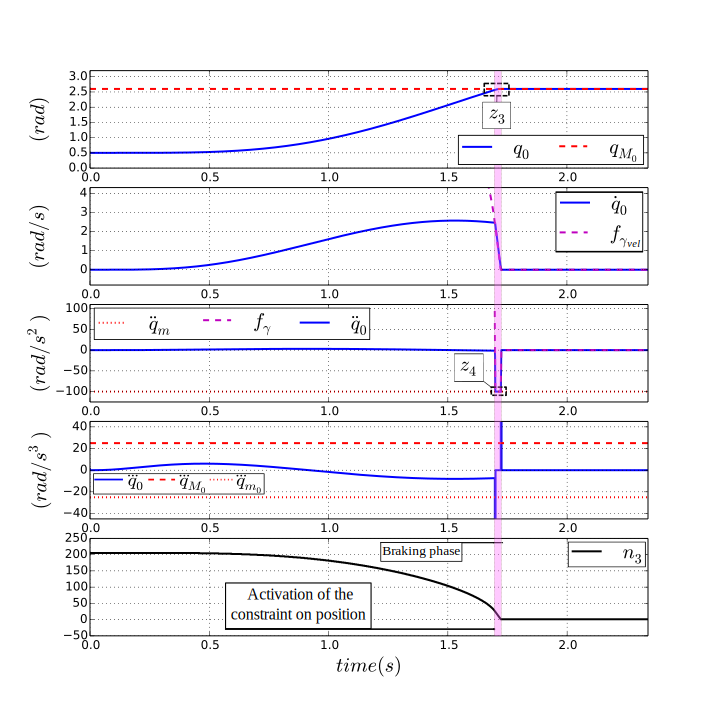
\includegraphics[width=0.8\columnwidth]{/home/anis/Desktop/THESIS_ANIS/THESIS/figures/Constrcomp/4_Posi_constr_acc_comp_100}}
%\caption{State $S$ of joint $0$ during the braking phase to cope with a maximum position limit $\q_{M_{0}}$; The new constraint formulation (\ref{eq:q_ddot_posi_acc_comp_upp}) that takes into account the deceleration capability $\ddot{q}_{m_{0}} = -100~rad.s^{-2}$ is used. Top to bottom: position, velocity, acceleration, jerk and $n_3$} 
%\label{fig:4_Posi_constr_acc_comp_100}
%\end{figure}
%%5
%\begin{figure}[!htbp]
%\centering
%{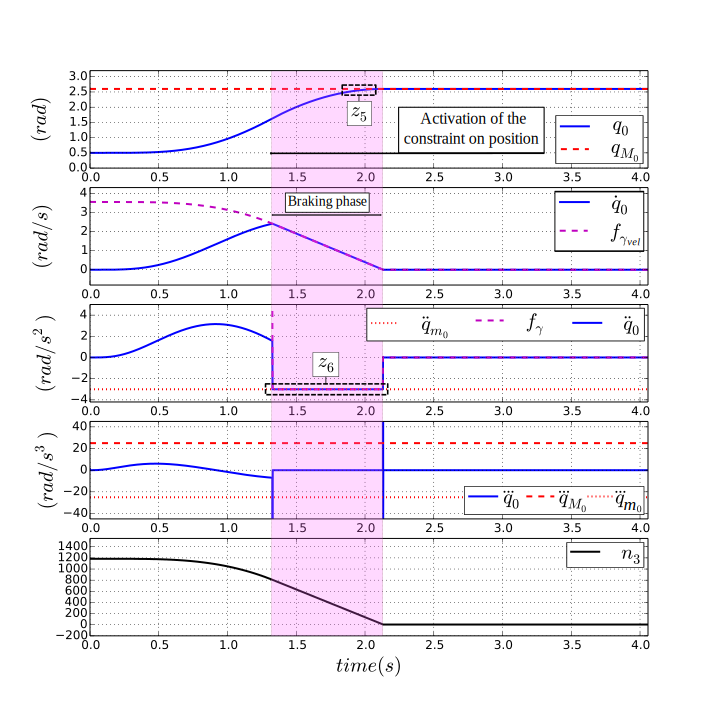
\includegraphics[width=0.8\columnwidth]{/home/anis/Desktop/THESIS_ANIS/THESIS/figures/Constrcomp/5_Posi_constr_acc_comp_3}}
%\caption{State $S$ of joint $0$ during the braking phase to cope with a maximum position limit; The new constraint formulation (\ref{eq:q_ddot_posi_acc_comp_upp}) that takes into account the deceleration capability $\ddot{q}_{m_{0}} = -3~rad.s^{-2}$ is used. Top to bottom: position, velocity, acceleration, jerk and $n_3$.} 
%\label{fig:5_Posi_constr_acc_comp_3}
%\end{figure}
%\begin{figure}[!htbp]
%\centering
%{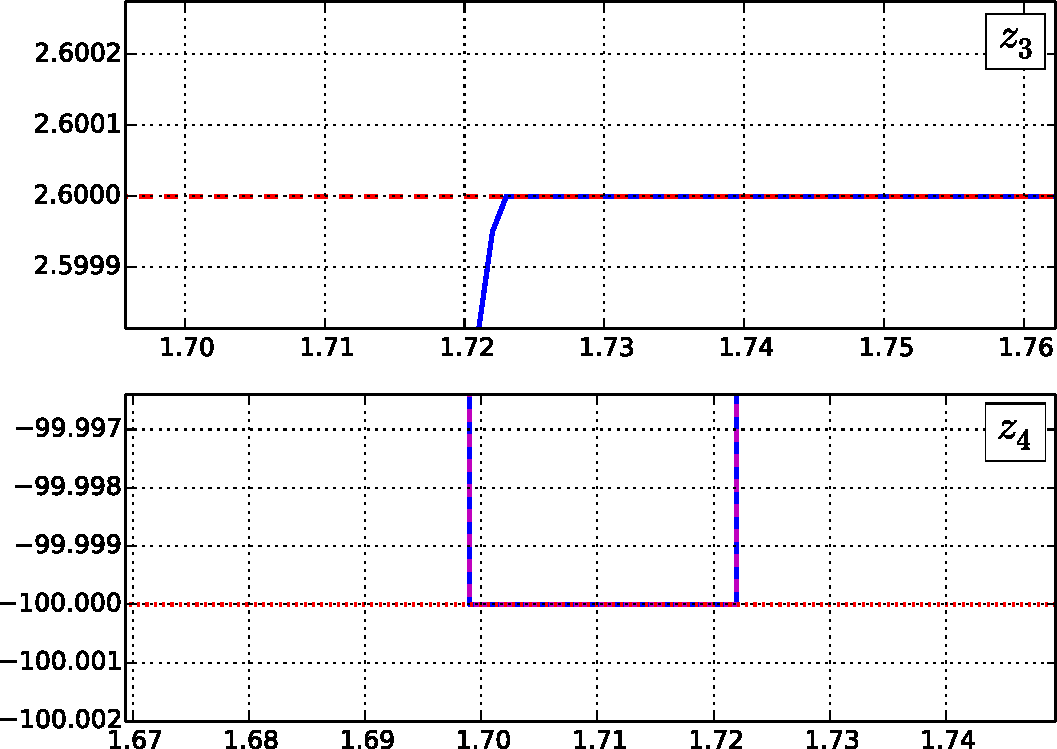
\includegraphics[width=0.8\columnwidth]{/home/anis/Desktop/THESIS_ANIS/THESIS/figures/Constrcomp/4_Posi_constr_acc_comp_100_zoom}}
%\caption{Zooms corresponding to Fig.~\ref{fig:4_Posi_constr_acc_comp_100}.} 
%\label{fig:4_Posi_constr_acc_comp_100_zoom}
%\end{figure}
%\begin{figure}[!htbp]
%\centering
%{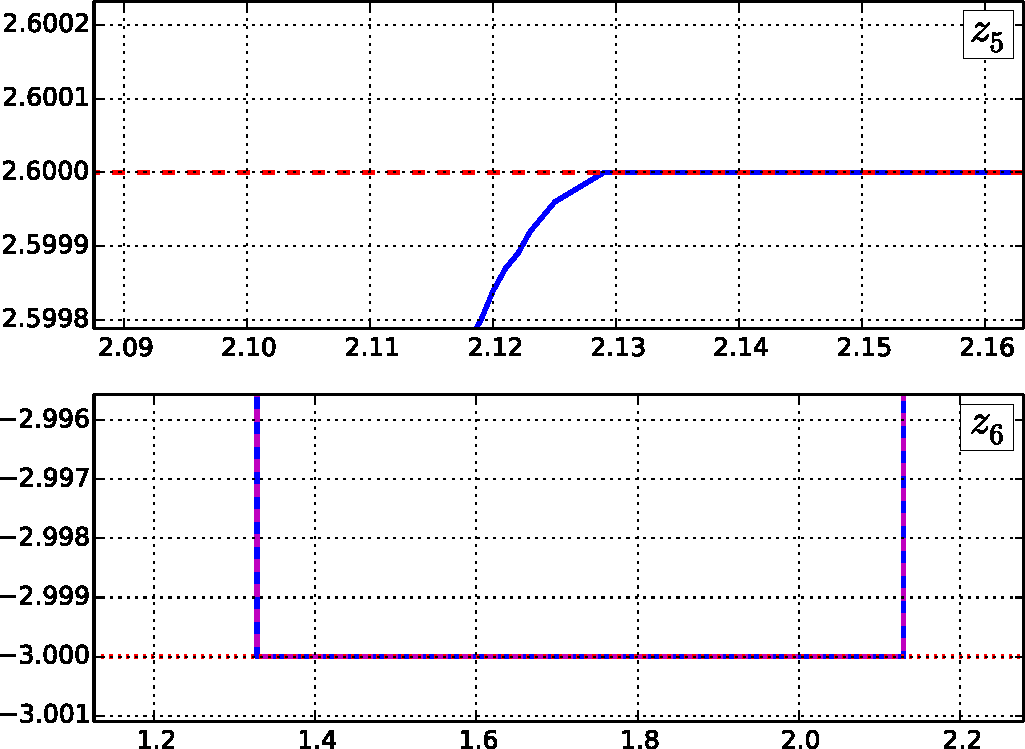
\includegraphics[width=0.8\columnwidth]{/home/anis/Desktop/THESIS_ANIS/THESIS/figures/Constrcomp/5_Posi_constr_acc_comp_3_zoom}}
%\caption{Zooms corresponding to Fig.~\ref{fig:5_Posi_constr_acc_comp_3}.} 
%\label{fig:5_Posi_constr_acc_comp_3_zoom}
%\end{figure}
\begin{landscape}
\begin{figure}
\begin{minipage}[c]{0.5\linewidth}
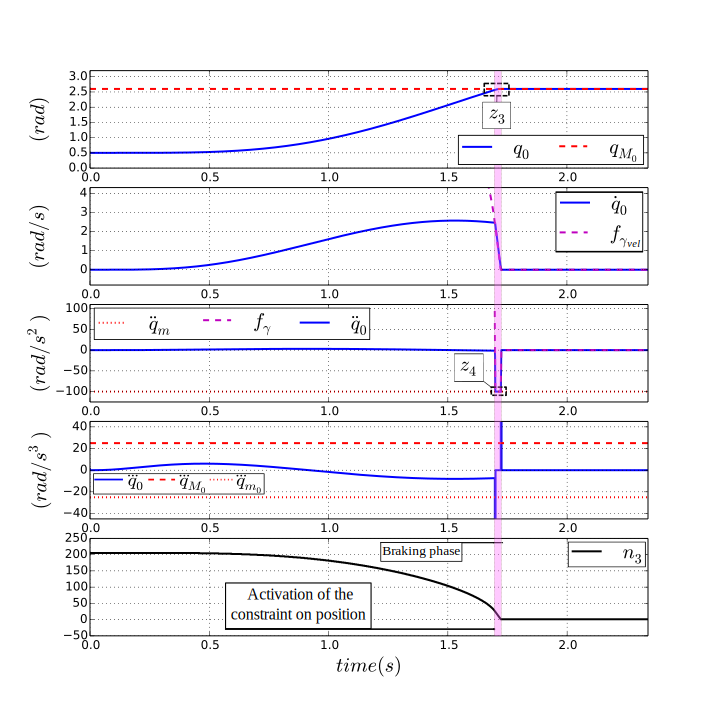
\includegraphics[width=0.99\columnwidth]{/home/anis/Desktop/THESIS_ANIS/THESIS/figures/Constrcomp/4_Posi_constr_acc_comp_100}
\caption{Extended state $S$ of joint $0$ during the braking phase implicitly induced by the joint's actuator to cope with the upper position limit $q_{M_{0}}$. The new formulation of the constraint on articular position (\ref{eq:q_ddot_posi_acc_comp_upp}) that takes into account the deceleration capability $\ddot{q}_{m_{0}} = -100~rad.s^{-2}$ is used. Top to bottom: position, velocity, acceleration, jerk and $n_3$. See $z_3$ and $z_4$ in Fig.~\ref{fig:4_Posi_constr_acc_comp_100_zoom}}.} 
\label{fig:4_Posi_constr_acc_comp_100}
\end{minipage}
\hfill
\begin{minipage}[c]{0.5\linewidth}
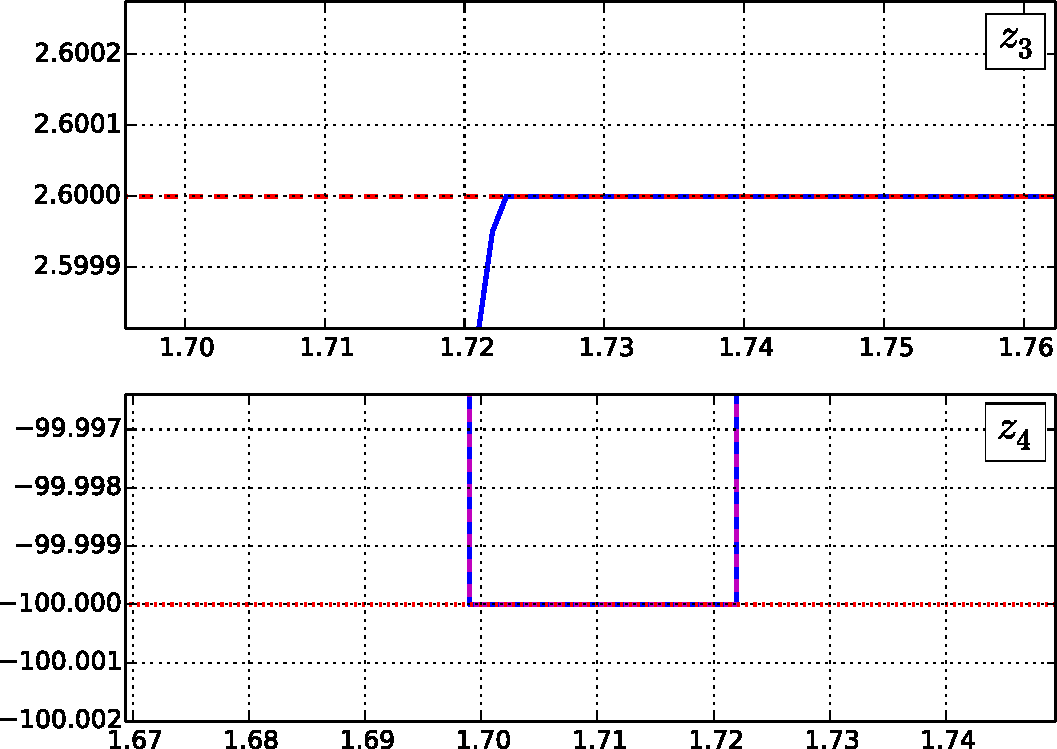
\includegraphics[width=0.90\columnwidth]{/home/anis/Desktop/THESIS_ANIS/THESIS/figures/Constrcomp/4_Posi_constr_acc_comp_100_zoom}
\caption{Zooms corresponding to Fig.~\ref{fig:4_Posi_constr_acc_comp_100}.} 
\label{fig:4_Posi_constr_acc_comp_100_zoom}
\end{minipage}%
\end{figure}
\end{landscape}
\begin{landscape}
\begin{figure}
\begin{minipage}[c]{0.5\linewidth}
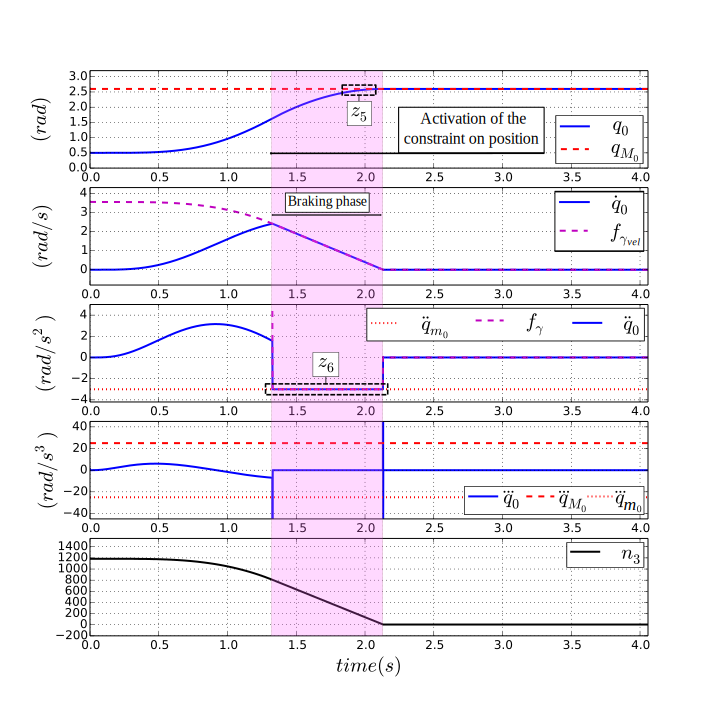
\includegraphics[width=0.99\columnwidth]{/home/anis/Desktop/THESIS_ANIS/THESIS/figures/Constrcomp/5_Posi_constr_acc_comp_3}
\caption{Extended state $S$ of joint $0$ during the braking phase implicitly induced by the joint's actuator to cope with the upper position limit $q_{M_{0}}$. The new formulation of the constraint on articular position (\ref{eq:q_ddot_posi_acc_comp_upp}) that takes into account the deceleration capability $\ddot{q}_{m_{0}} = -3~rad.s^{-2}$ is used. Top to bottom: position, velocity, acceleration, jerk and $n_3$. See $z_5$ and $z_6$ in Fig.~\ref{fig:5_Posi_constr_acc_comp_3_zoom}}.} 
\label{fig:5_Posi_constr_acc_comp_3}
\end{minipage}
\hfill
\begin{minipage}[c]{0.5\linewidth}
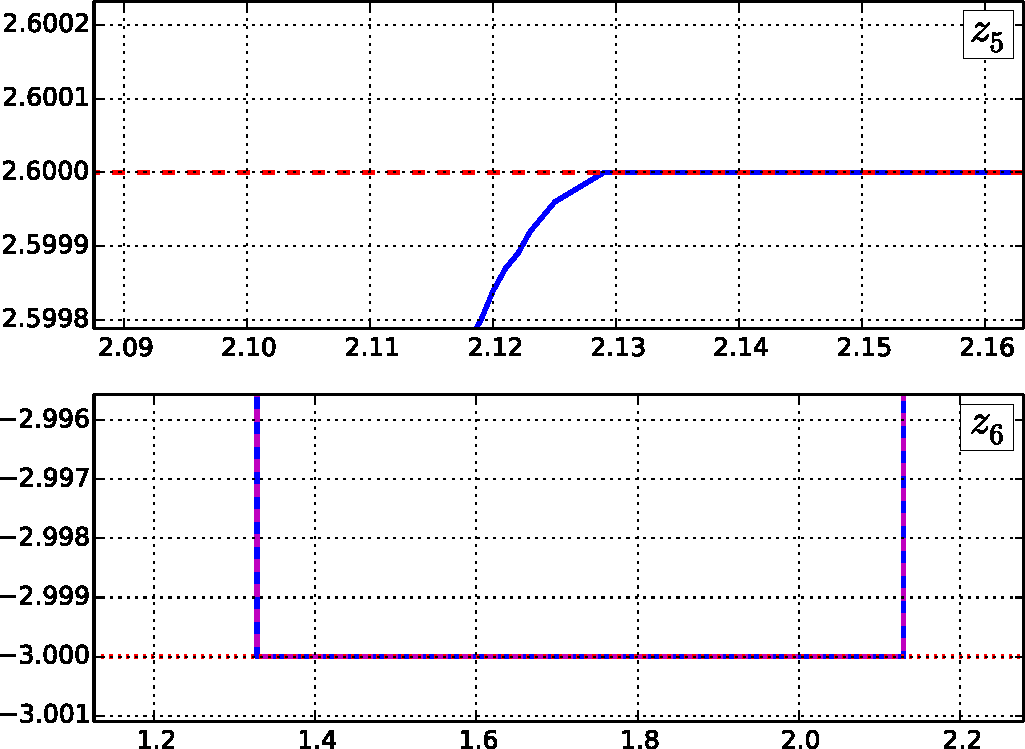
\includegraphics[width=0.90\columnwidth]{/home/anis/Desktop/THESIS_ANIS/THESIS/figures/Constrcomp/5_Posi_constr_acc_comp_3_zoom}
\caption{Zooms corresponding to Fig.~\ref{fig:5_Posi_constr_acc_comp_3}.} 
\label{fig:5_Posi_constr_acc_comp_3_zoom}
\end{minipage}%
\end{figure}
\end{landscape}
%%%%%%%%%%%%%%%%%%%%%%%%%%SUBSUBSECTION%%%%%%%%%%%%%%%%%%%%%%%%%%%%%
%%%%%%%%%%%%%%%%%%%%%%%%%%SUBSUBSECTION%%%%%%%%%%%%%%%%%%%%%%%%%%%%%
\subsubsection{Joint position constraint incompatibility with jerk limits 1}
\label{sec:secref2}
We consider a braking phase for a joint moving towards its upper position limit $q_M$. In this case, only the lower limit $\dddot{q}_m$ of jerk capabilities is considered. Maximum producible deceleration $\ddot{q}_m$ is not taken into account. The extended state \textit{S} of the system during this implicitly induced braking phase, that makes the joint's actuator stop at its upper position limit $q_M$, can be described as: 
\begin{equation} 
\begin{split}
\textit{S}_{|k+1}&\left\{\begin{array}{lcl}
q_{|k+1} \hspace{2mm}= q_{|k} + \dot{q}_{|k} \delta t, \\
\dot{q}_{|k+1} \hspace{2mm}= \dot{q}_{|k} + \ddot{q} \delta t, \\
\ddot{q}_{|k+1} \hspace{2mm}= \ddot{q}_{|k} + \dddot{q}_{m} \delta t;
\end{array}\right.\\
\textit{S}_{|k+2}&\left\{\begin{array}{lcl}
q_{|k+2} \hspace{2mm}= q_{|k+1} + \dot{q}_{|k+1} \delta t, \\
\dot{q}_{|k+2} \hspace{2mm}= \dot{q}_{|k+1} + \ddot{q}_{|k+1} \delta t, \\
\ddot{q}_{|k+2} \hspace{2mm}= \ddot{q}_{|k+1} + \dddot{q}_{m} \delta t;
\end{array}\right.\\
& \hspace{7mm}\vdots\ \hspace{13mm}\vdots\ \\
\textit{S}_{|k+n_{5}}&\left\{\begin{array}{lcl}
q_{|k+n_{5}} = q_{|k+n_{5}-1} + \dot{q}_{|k+n_{5}-1} \delta t, \\
\dot{q}_{|k+n_{5}} = \dot{q}_{|k+n_{5}-1} + \ddot{q}_{|k+n_{5}-1} \delta t, \\
\ddot{q}_{|k+n_{5}} = \ddot{q}_{|k+n_{5}-1} + \dddot{q}_{m} \delta t.
\end{array}\right.
\end{split}
\label{eq:discretized_dynamics_posi_jerk_braking}
\end{equation}
With: $q_{|k} \geq 0$, $\dot{q}_{|k} \geq 0$ and  $\dddot{q}_{m} \leq 0$. The joint position evolution within $n_5$ iterations is equal to the general form\footnote{Computed using Maple \cite{maple}.} of the numerical sequence (\ref{eq:discretized_dynamics_posi_jerk_braking}):
\begin{equation}
q_{|k+n_5} = q_{|k} + n_5 \dot{q}_{|k} \delta t +  \frac{\left(n_5^2-n_5\right)}{2} \ddot{q}_{|k} \delta t^2 + \left(\frac{n_5^3}{6}-\frac{n_5^2}{2}+\frac{n_5}{3}\right) \dddot{q}_m \delta t^3.
\label{eq:q_evolution_with_const_qdddot_m}
\end{equation}
The condition $q_{|k+n_5} \leq q_{M}$ for all integer $n_5$ leads to:
\begin{equation}
\begin{split}
\ddot{q}_{|k}^{c} \leq \frac{2\left(q_M-q_{|k}\right)}{\left(n_5^2-n_5\right) \delta t^2} - \frac{2 \dot{q}_{|k}}{\left(n_5-1\right) \delta t} - \frac{\left(\frac{n_5^2}{3}-n_5+\frac{2}{3}\right)}{\left(n_5-1\right)}\dddot{q}_m \delta t,
\label{eq:q_ddot_posi_jerk_comp_upp}
\end{split}
\end{equation}
with $n_5$, the integer minimizing the right-hand side of (\ref{eq:q_ddot_posi_jerk_comp_upp}). It can be computed analytically. By differentiating this expression w.r.t $n_5$:
\begin{equation}
\left\{\begin{array}{lcl}
n_5 \geq 3, \\
\begin{split}
-&\left(\frac{1}{3} \dddot{q}_m \delta t^3\right) n_5^4 + \left(\frac{2}{3} \dddot{q}_{|m} \delta t^3\right) n_5^3  \\
+&\left(2 \dot{q}_{|k} \delta t - \frac{1}{3} \dddot{q}_m \delta t^3\right) n_5^2 \\
+& 4 \left(q_M-q_{|k}\right) n_5 - 2\left(q_M-q_{|k}\right)=0.
\end{split}
\end{array}\right.
\label{eq:n_5_eq_new}
\end{equation}
$n_5$ is the rounded-up real root of (\ref{eq:n_5_eq_new}). It must be $\geq 3$ so that $\dddot{q}_m$ is always part of (\ref{eq:q_ddot_posi_jerk_comp_upp})\\
Following the same reasoning for the lower position limit, the condition $q_{|k+n_6} \geq q_{m}$ for all integer $n_6 \geq 3$ can be reflected on the acceleration control variable as:
\begin{equation}
\begin{split}
\ddot{q}_{|k}^{c}  \geq \frac{2(q_m - q_{|k})}{\left(n_6^2 - n_6\right)\delta t^2} - \frac{2 \dot{q}_{|k}}{(n_6-1)\delta t} 
- \frac{\left(\frac{n_6^2}{3} - n_6 + \frac{2}{3}\right)}{(n_6-1)}\dddot{q}_M \delta t
\label{eq:q_ddot_posi_jerk_comp_low}
\end{split}
\end{equation}
With: 
\begin{equation}
\left\{\begin{array}{lcl}
n_6 \geq 3, \\
\begin{split}
-&\left(\frac{1}{3} \dddot{q}_M \delta t^3\right) n_6^4 + \left(\frac{2}{3} \dddot{q}_{|M} \delta t^3\right) n_6^3  \\
+&\left(2 \dot{q}_{|k} \delta t - \frac{1}{3} \dddot{q}_M \delta t^3\right) n_6^2 \\
+& 4 \left(q_m-q_{|k}) n_6 - 2(q_m-q_{|k}\right)=0.
\end{split}
\end{array}\right.
\label{eq:n_6_eq_new}
\end{equation}
$n_6$ is the rounded up real root of (\ref{eq:n_6_eq_new}) that maximizes the right-hand side of (\ref{eq:q_ddot_posi_jerk_comp_low}). We recall that: $n_5$ is the number of control time-steps corresponding to the duration of a braking phase implicitly induced by an actuator moving towards its upper position limit $q_M$, and during which both its acceleration and velocity are brought to zero by jerking with maximum negative producible jerk $\dddot{q}_m$ and; $n_6$ is the number of control time-steps corresponding to the duration of a braking phase implicitly induced by an actuator moving towards its lower position limit $q_m$, and during which both its acceleration and velocity are brought to zero by jerking with maximum positive producible jerk $\dddot{q}_M$. \\
$\textit{f}_{\theta}$ and $\textit{f}_{\eta}$ are respectively equivalent to the right-hand sides of (\ref{eq:q_ddot_posi_jerk_comp_low}) and (\ref{eq:q_ddot_posi_jerk_comp_upp}). \\
\noindent\begin{minipage}{\textwidth}
\renewcommand\footnoterule{}                  %% This line should come here.
\begin{algorithm}[H]
\caption{Compute $n_{5}, n_{6}, f_{\theta}$ and $f_{\eta}$}
\label{alg:compute_f_theta_f_eta_n_5_n_6}
\begin{algorithmic}[1]
%f_{\theta}(n_{6})     f_{\eta}(n_{5})
%    n1_pos         n1_neg 
\Require $q_M, q_m, q_{|k}, \dot{q}_{|k},\dddot{q}_{M},\dddot{q}_{m}, \delta t$
\myState{$f_{{\theta}_{max}} \gets \ddot{q}_{m}$} \Comment{temporary lower bound of $\ddot{q}_{|k}^{c}$}
\myState{$f_{{\eta}_{min}} \gets \ddot{q}_{M}$} \Comment{temporary upper bound of $\ddot{q}_{|k}^{c}$}
\For{($i = 3 \rightarrow N$)}
        \myState{$n_{5}^{*} \gets i \qquad n_{6}^{*} \gets i$}
        \myState{$f_{\theta}^{*} \gets f_{\theta}(q_m, \dddot{q}_M, q_{|k}, \dot{q}_{|k}, \dddot{q}_M, n_{6}^{*})$} 
        \myState{$f_{\eta}^{*} \gets f_{\eta}(q_M, \dddot{q}_m, q_{|k}, \dot{q}_{|k}, \dddot{q}_m, n_{5}^{*})$}
        \If{($f_{\theta}^{*} \geq f_{{\theta}_{max}}$)}
            \State{$f_{{\theta}_{max}} \gets f_{\theta}^{*} \qquad n_{6} \gets n_{6}^{*} $}
        \EndIf   
        \If{($f_{\eta}^{*} \leq f_{{\eta}_{min}}$)}
            \State{$f_{{\eta}_{min}} \gets f_{\eta}^{*} \qquad n_{5} \gets n_{5}^{*}$}
        \EndIf            
\EndFor
\State{$f_{\theta} \gets f_{{\theta}_{max}} \qquad f_{\eta} \gets f_{{\eta}_{min}}$}
\myState \Return{$n_{5}, n_{6}, f_{\theta}, f_{\eta}$}\;
\end{algorithmic}
\end{algorithm}
\end{minipage} \\
\\
Finally, $n_{5}, n_{6}, f_{\theta}$ and $f_{\eta}$ can be computed numerically as shown by Algorithm~\ref{alg:compute_f_theta_f_eta_n_5_n_6}. 
N in Algorithm~\ref{alg:compute_f_theta_f_eta_n_5_n_6} can be fixed heuristically, it must be however $\geq$ to the solutions of (\ref{eq:n_5_eq_new}) and (\ref{eq:n_6_eq_new}). More details on how to compute this parameter in Section~\ref{sec:concl_comp_cnstr}.
%********************************************************************%
\paragraph{Illustration 3}
For this simulation, using the test case scenario, the controller is implemented with the new formulation of the constraint on articular position  (\ref{eq:q_ddot_posi_jerk_comp_upp}), that takes into account the available jerk capability $(\dddot{q}_{m_{0}} = -25~rad.s^{-3})$. The right-hand side of the constraint on articular jerk (\ref{eq:cnt_lit_tme_step_4}) $(\dddot{q}_{{0}_{|k}} \leq \dddot{q}_{M_{0}} = 25~rad.s^{-3})$ is also included in the configuration of the controller. As for the previous simulations, joint $0$ moves towards its upper position limit $q_{M_{0}}$. 

Fig.~\ref{fig:6_Posi_constr_jerk_comp_25_non_complete_formula_backklash} illustrates how joint $0$ starts braking with maximum negative jerk $\dddot{q}_{m_{0}}$ until its upper position limit is reached. The amount of ``\textit{charged}'' deceleration should then be brought to $0$. However, because of the constraint on articular jerk, the amount of deceleration \textit{loaded} in the joint cannot be ``\textit{de-charged}'' instantaneously. The joint is then forced to move away from $q_{M_{0}}$ and oscillates until completely and progressively ``\textit{de-charging}'' the amount of deceleration $(\ddot{q}_{m_{0}} \leq 0)$ it contains. \\
On the other hand, in case of an actuator with higher jerk capabilities (e.g., $\dddot{q}_{m_{0}} = -2500 ~rad.s^{-3}$), the decaying oscillations can be quite reduced (see Fig.~\ref{fig:7_Posi_constr_jerk_comp_2500_non_complete_formula_backklash}).
This makes the proposed new formulation of the constraint on articular position more convenient when using actuators that can generate larger amounts of jerk. The maximum amplitude of the induced oscillations is noticeably diminished: from $0.8~rad$ in Fig.~\ref{fig:6_Posi_constr_jerk_comp_25_non_complete_formula_backklash} to $0.025~rad$ in Fig.~\ref{fig:7_Posi_constr_jerk_comp_2500_non_complete_formula_backklash}. Note that the main reason for these oscillations is the non-\nameref{label:complete} description of the braking phase in (\ref{eq:discretized_dynamics_posi_jerk_braking}). Indeed,  the \textit{deceleration de-charging with positive jerk} sub-phase (sub-phase \circled{3} in Fig.~\ref{fig:per_Pr_jerk_ala_3}) is not considered in this version of the formulation of the articular position constraint. Also, as is it appears in Fig.~\ref{fig:6_Posi_constr_jerk_comp_25_non_complete_formula_backklash_zoom} and Fig.~\ref{fig:7_Posi_constr_jerk_comp_2500_non_complete_formula_backklash_zoom},  the lower jerk limit is not perfectly satisfied. This is mainly due to the \textit{discrete} description (\ref{eq:discretized_dynamics_posi_jerk_braking}) of the state of the joint during the braking phase. In such case, including the \textit{hard-coded} constraint (\ref{eq:cnt_lit_tme_step_4}) on the negative articular jerk $(\dddot{q}_{0_{|k}} \geq\dddot{q}_{m_{0}} = -25~rad.s^{-3})$ in the configuration of the controller will inevitably result into an infeasible control problem. 
%\begin{figure}[!htbp]
%\centering
%{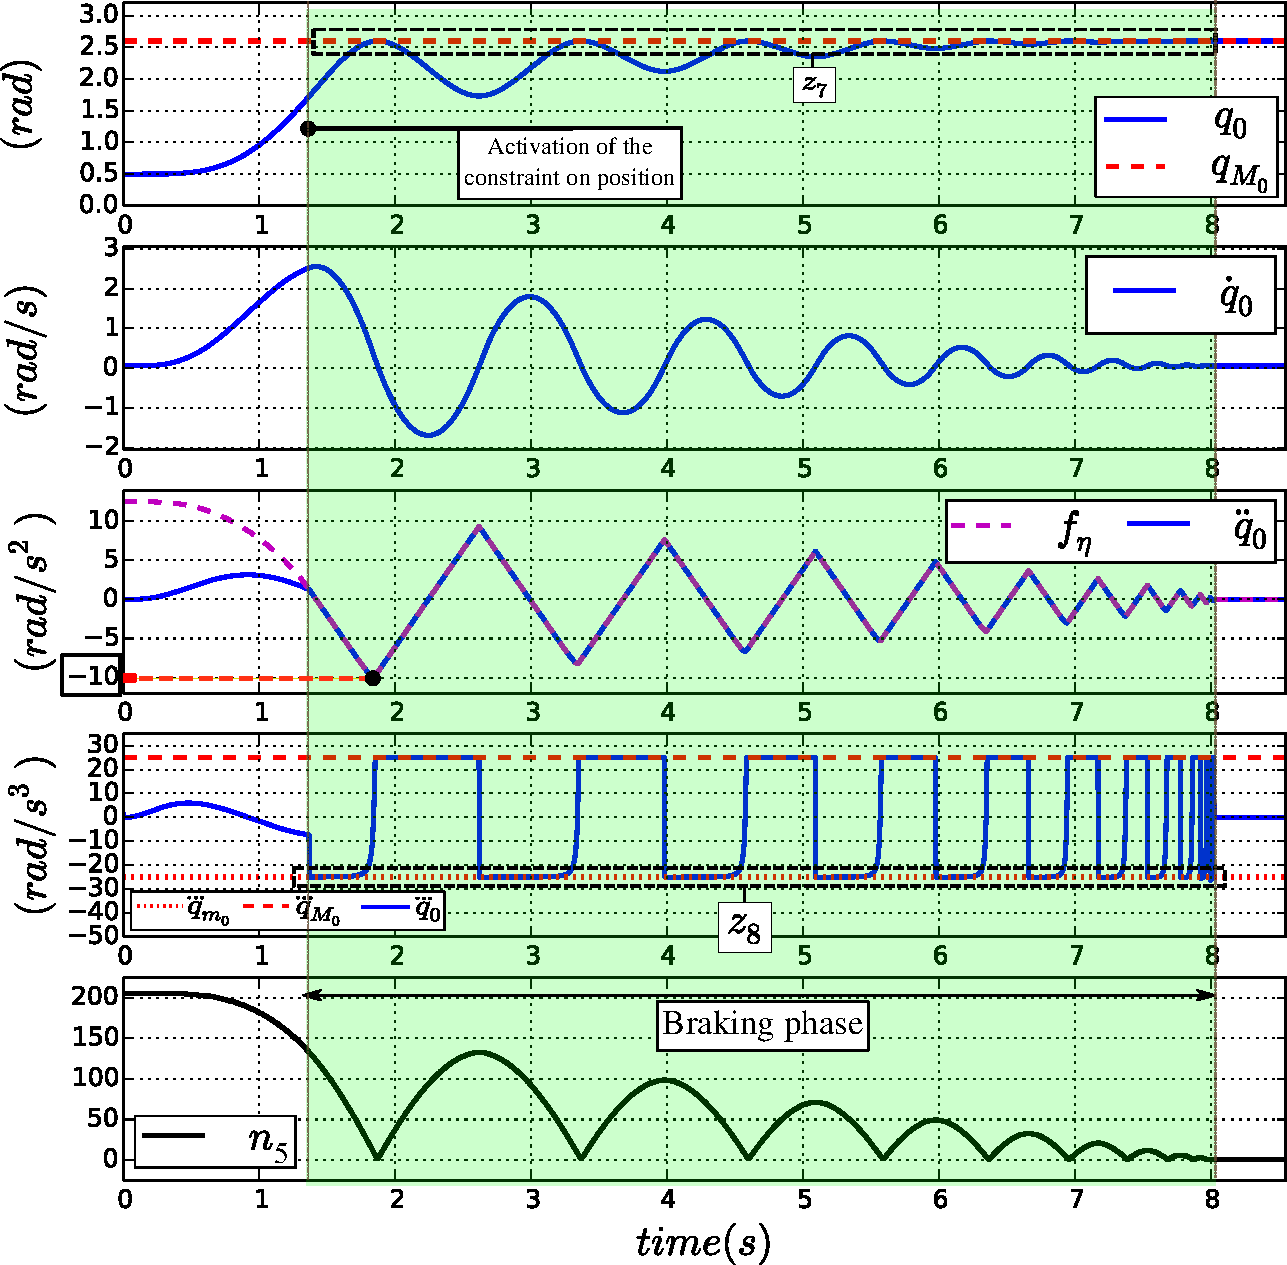
\includegraphics[width=0.8\columnwidth]{/home/anis/Desktop/THESIS_ANIS/THESIS/figures/Constrcomp/6_Posi_constr_jerk_comp_25_non_complete_formula_backklash}}
%\caption{State $S$ of joint $0$ during the braking phase to cope with a maximum position limit $q_{M_{0}}$; The new constraint formulation (\ref{eq:q_ddot_posi_jerk_comp_upp}) that takes into account the jerk capability $\dddot{q}_{m_{0}} = -25~rad.s^{-3}$ is used. Top to bottom: position, velocity, acceleration, jerk and $n_5$.} 
%\label{fig:6_Posi_constr_jerk_comp_25_non_complete_formula_backklash}
%\end{figure}
%\begin{figure}[!htbp]
%\centering
%{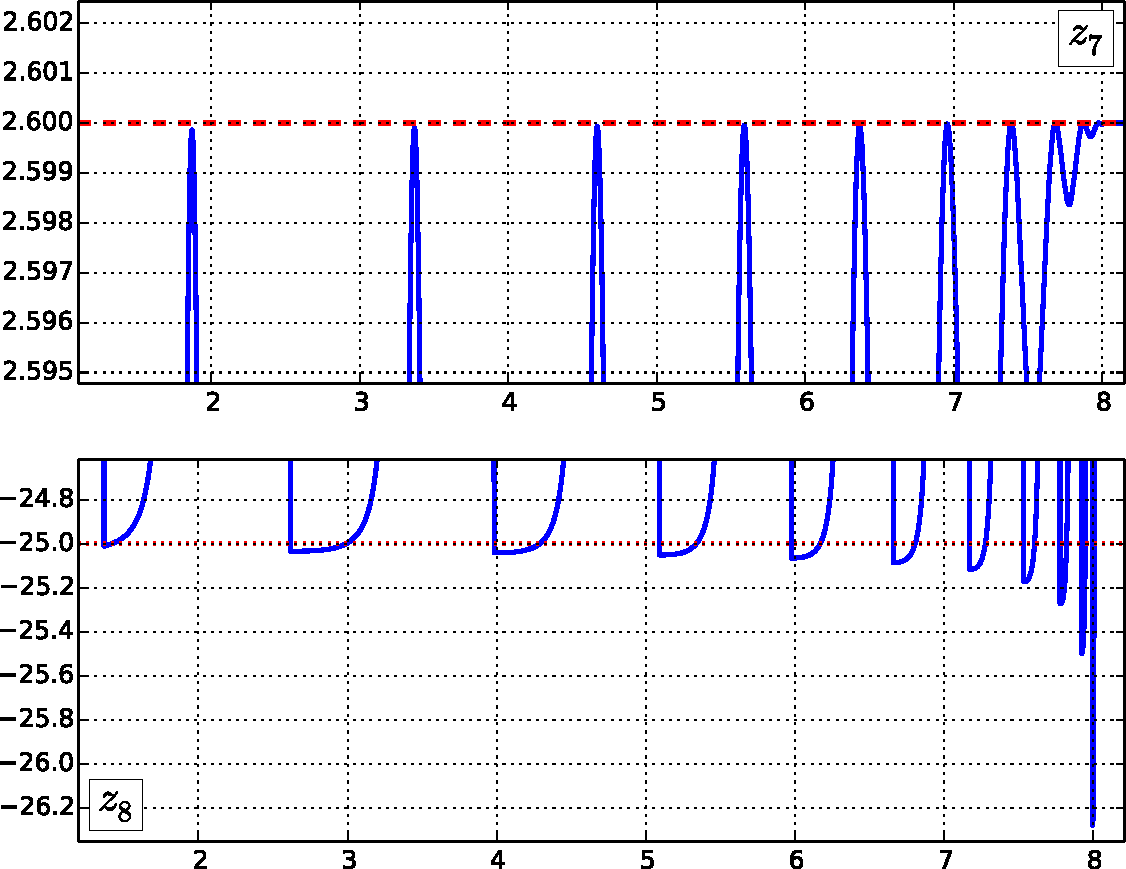
\includegraphics[width=0.8\columnwidth]{/home/anis/Desktop/THESIS_ANIS/THESIS/figures/Constrcomp/6_Posi_constr_jerk_comp_25_non_complete_formula_backklash_zoom}}
%\caption{Zooms corresponding to Fig.~\ref{fig:6_Posi_constr_jerk_comp_25_non_complete_formula_backklash}.} 
%\label{fig:6_Posi_constr_jerk_comp_25_non_complete_formula_backklash_zoom}
%\end{figure}
\begin{landscape}
\begin{figure}
\begin{minipage}[c]{0.5\linewidth}
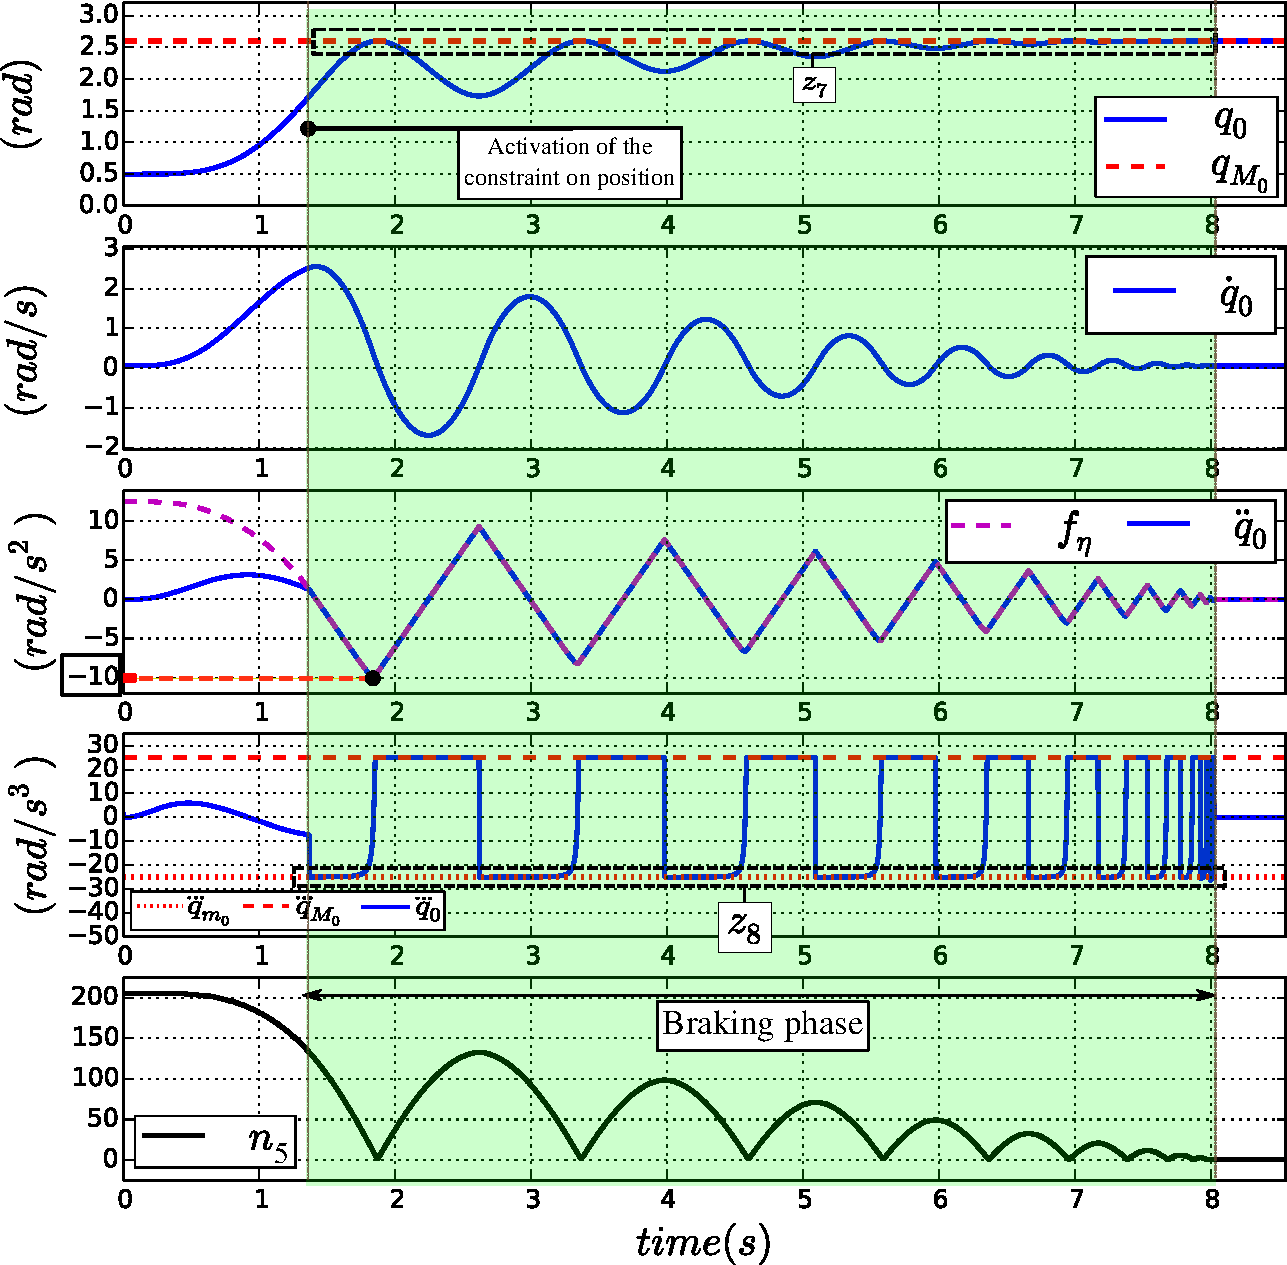
\includegraphics[width=0.99\columnwidth]{/home/anis/Desktop/THESIS_ANIS/THESIS/figures/Constrcomp/6_Posi_constr_jerk_comp_25_non_complete_formula_backklash}
\caption{Extended state $S$ of joint $0$ during the braking phase implicitly induced to cope with an upper position limit $q_{M_{0}}$. The new version of the formulation of the constraint on articular position (\ref{eq:q_ddot_posi_jerk_comp_upp}) that takes into account the jerk capability $(\dddot{q}_{m_{0}} = -25~rad.s^{-3})$ is used. Top to bottom: position, velocity, acceleration, jerk and $n_5$. See $z_7$ and $z_8$ in Fig.~\ref{fig:4_Posi_constr_acc_comp_100_zoom}.} 
\label{fig:6_Posi_constr_jerk_comp_25_non_complete_formula_backklash}
\end{minipage}
\hfill
\begin{minipage}[c]{0.5\linewidth}
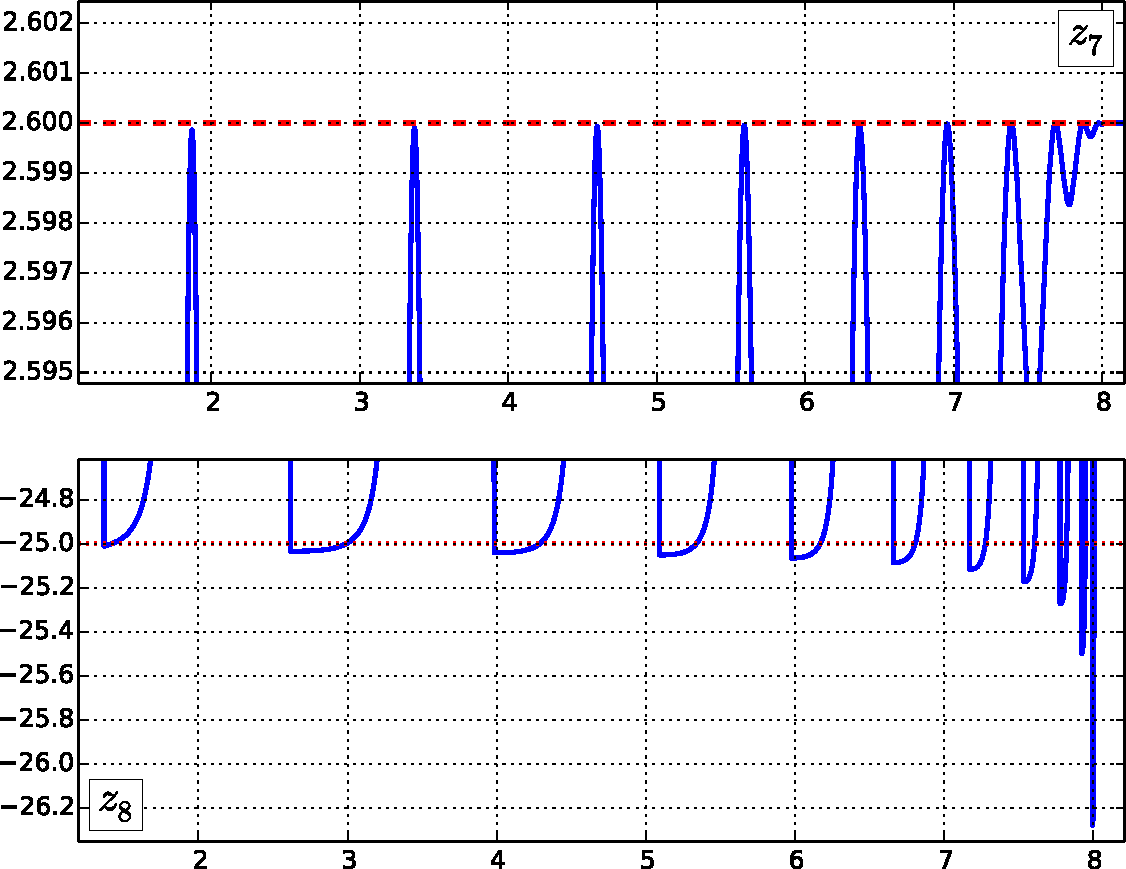
\includegraphics[width=0.90\columnwidth]{/home/anis/Desktop/THESIS_ANIS/THESIS/figures/Constrcomp/6_Posi_constr_jerk_comp_25_non_complete_formula_backklash_zoom}
\caption{Zooms corresponding to Fig.~\ref{fig:6_Posi_constr_jerk_comp_25_non_complete_formula_backklash}.} 
\label{fig:6_Posi_constr_jerk_comp_25_non_complete_formula_backklash_zoom}
\end{minipage}%
\end{figure}
\end{landscape}
%7
%\begin{figure}[!htbp]
%\centering
%{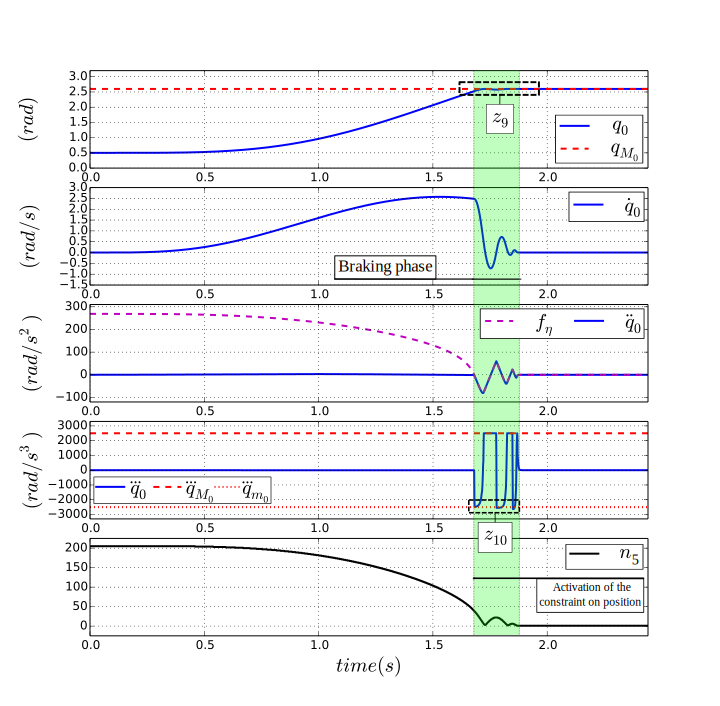
\includegraphics[width=0.8\columnwidth]{/home/anis/Desktop/THESIS_ANIS/THESIS/figures/Constrcomp/7_Posi_constr_jerk_comp_2500_non_complete_formula_backklash}}
%\caption{State $S$ of joint $0$ during the braking phase to cope with a maximum position limit; The new constraint formulation (\ref{eq:q_ddot_posi_jerk_comp_upp}) that takes into account the jerk capability $\dddot{q}_{m_{0}} = -2500~rad.s^{-3}$. Top to bottom: position, velocity, acceleration, jerk and $n_5$.} 
%\label{fig:7_Posi_constr_jerk_comp_2500_non_complete_formula_backklash}
%\end{figure}
%\begin{figure}[!htbp]
%\centering
%{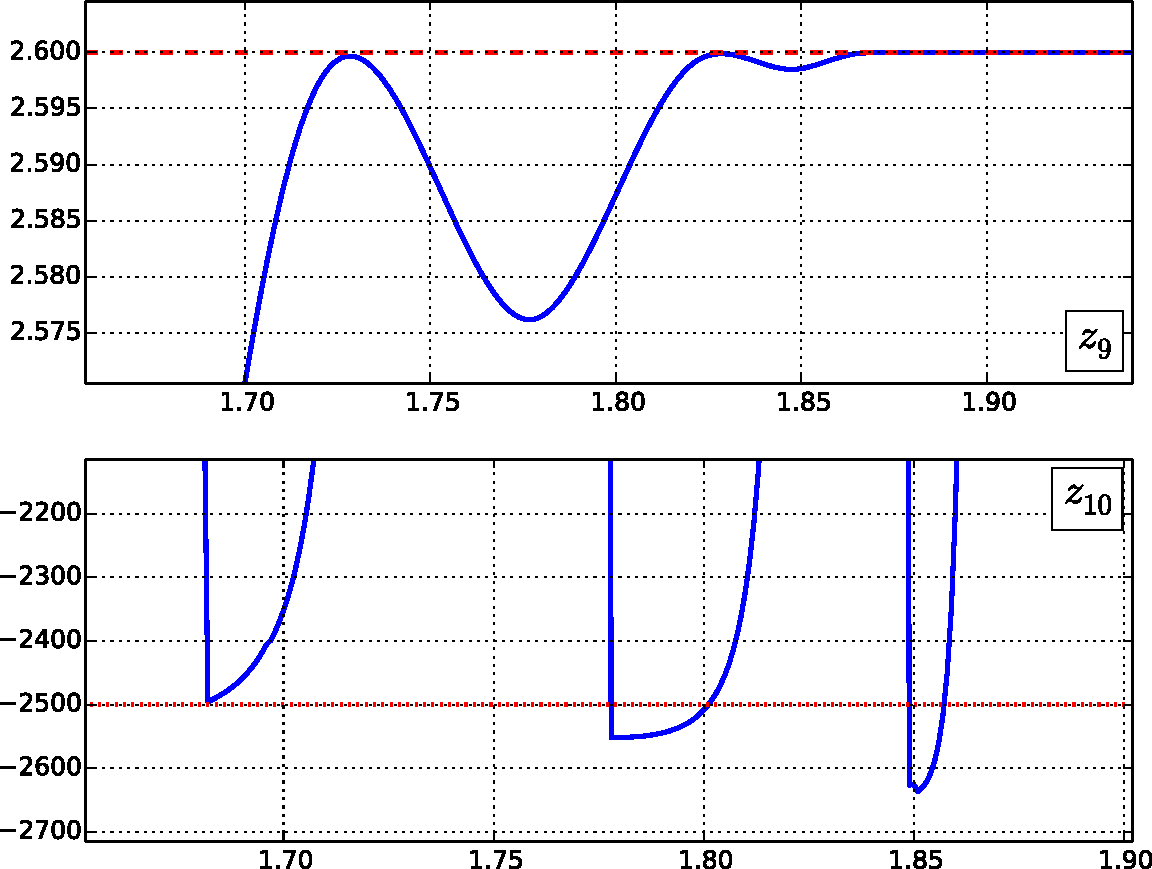
\includegraphics[width=0.7\columnwidth]{/home/anis/Desktop/THESIS_ANIS/THESIS/figures/Constrcomp/7_Posi_constr_jerk_comp_2500_non_complete_formula_backklash_zoom}}
%\caption{Zooms corresponding to Fig.~\ref{fig:7_Posi_constr_jerk_comp_2500_non_complete_formula_backklash}.} 
%\label{fig:7_Posi_constr_jerk_comp_2500_non_complete_formula_backklash_zoom}
%\end{figure}
\begin{landscape}
\begin{figure}
\begin{minipage}[c]{0.5\linewidth}
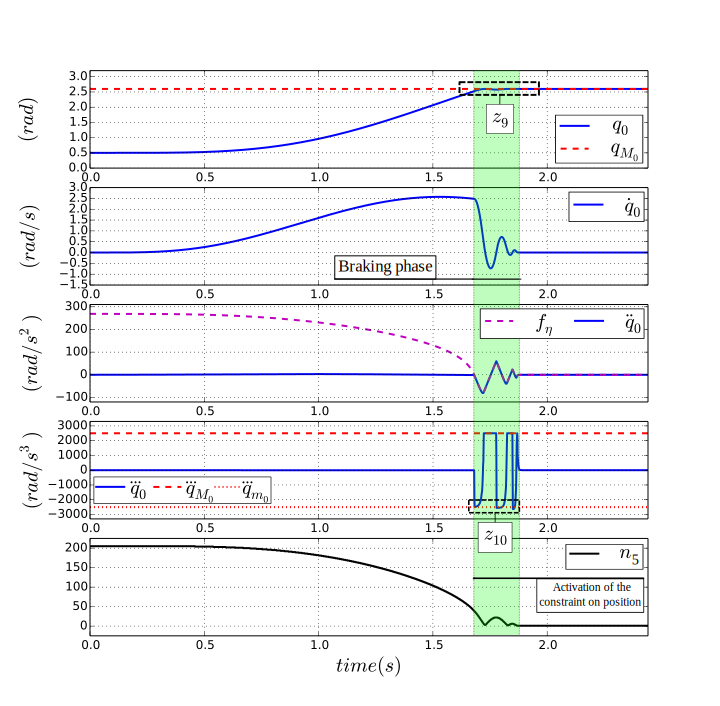
\includegraphics[width=0.99\columnwidth]{/home/anis/Desktop/THESIS_ANIS/THESIS/figures/Constrcomp/7_Posi_constr_jerk_comp_2500_non_complete_formula_backklash}
\caption{Extended state $S$ of joint $0$ during the braking phase implicitly induced to cope with an upper position limit $q_{M_{0}}$. The new version of the formulation of the constraint on articular position (\ref{eq:q_ddot_posi_jerk_comp_upp}) that takes into account the jerk capability $(\dddot{q}_{m_{0}} = -2500~rad.s^{-3})$ is used. Top to bottom: position, velocity, acceleration, jerk and $n_5$. See $z_9$ and $z_{10}$ in Fig.~\ref{fig:7_Posi_constr_jerk_comp_2500_non_complete_formula_backklash_zoom}.} 
\label{fig:7_Posi_constr_jerk_comp_2500_non_complete_formula_backklash}
\end{minipage}
\hfill
\begin{minipage}[c]{0.5\linewidth}
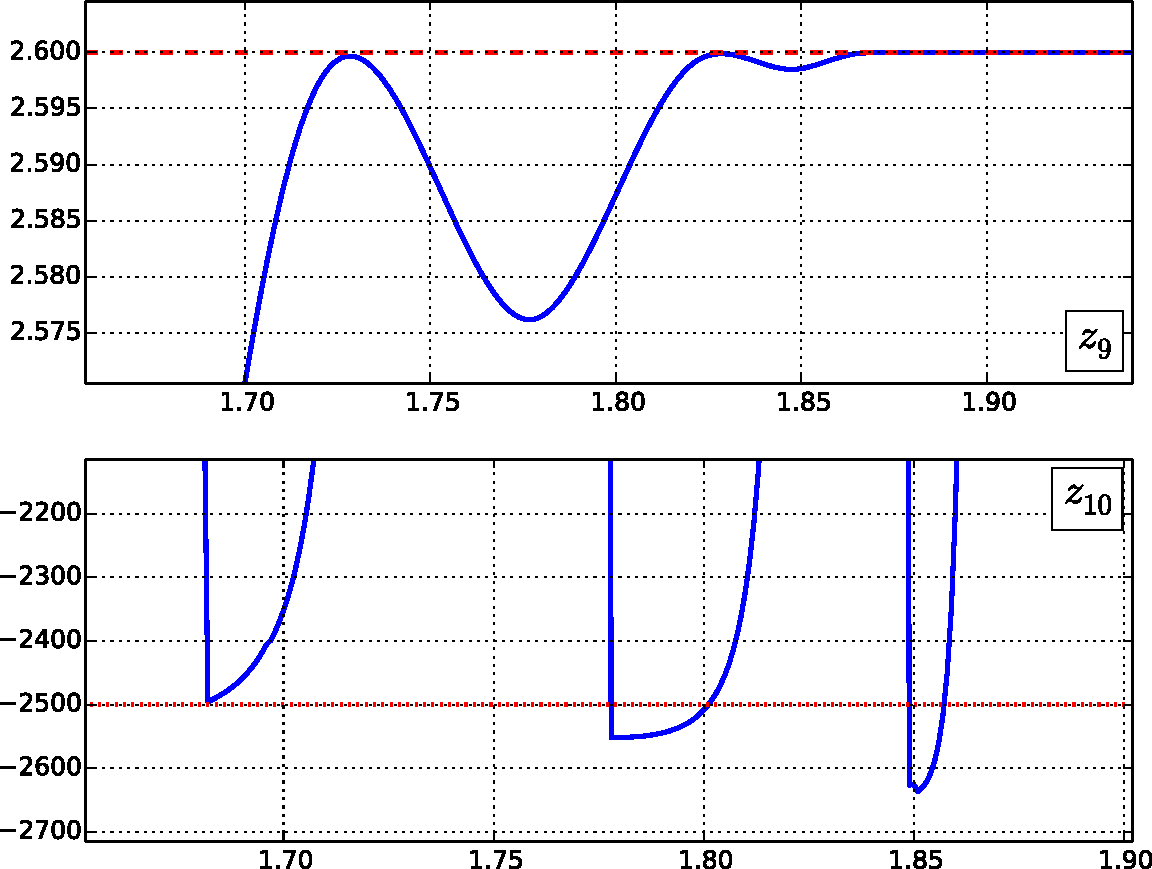
\includegraphics[width=0.90\columnwidth]{/home/anis/Desktop/THESIS_ANIS/THESIS/figures/Constrcomp/7_Posi_constr_jerk_comp_2500_non_complete_formula_backklash_zoom}
\caption{Zooms corresponding to Fig.~\ref{fig:7_Posi_constr_jerk_comp_2500_non_complete_formula_backklash}.} 
\label{fig:7_Posi_constr_jerk_comp_2500_non_complete_formula_backklash_zoom}
\end{minipage}%
\end{figure}
\end{landscape}
%%%%%%%%%%%%%%%%%%%%%%%%%%SUBSUBSECTION%%%%%%%%%%%%%%%%%%%%%%%%%%%%%
%%%%%%%%%%%%%%%%%%%%%%%%%%SUBSUBSECTION%%%%%%%%%%%%%%%%%%%%%%%%%%%%%
\subsubsection{Joint position constraint incompatibility with jerk limits 2}
\label{subsec:case3}
As previously explained, to palliate the oscillations induced on the movement of a joint when using (\ref{eq:qddot_cond_to_satisfy_Jerk_posi_compatibility}) to cope with an upper or lower position limit, a more \nameref{label:complete} description of the braking phase must be used. In this case, we consider the braking phase of a joint moving towards its upper position limit $q_{M}$, the new formulation of the constraint on its position includes both the lower $\dddot{q}_{m}$ and upper $\dddot{q}_{M}$ jerk limits. The implicitly induced braking phase that makes the joint stop at $q_{M}$ is as follows: joint $0$ starts jerking negatively with maximum producible jerk $\dddot{q}_m$ during $n_{7}$ iterations to force reduce the amount of acceleration $(\ddot{q} \geq 0)$ it contains. The reached amount of deceleration $(\ddot{q} \leq 0)$ is then progressively ``\textit{released}'' and brought to $0$ by jerking positively with maximum producible jerk $\dddot{q}_M$ during $n_{9}$ control time-steps (see Fig.~\ref{fig:8_Podfgf12}). Maximum producible deceleration $\ddot{q}_{m}$ is not considered in this case. The extended state $\textit{S}$ of the system during this implicitly induced braking phase can be described as:
\begin{equation} 
\resizebox{0.63\hsize}{!}{$
\begin{split}
\left.\begin{aligned}
\textit{S}_{|k+1}&\left\{\begin{array}{lcl}
q_{|k+1} \hspace{5mm}= q_{|k} + \dot{q}_{|k} \delta t, \\
\dot{q}_{|k+1} \hspace{5mm}= \dot{q}_{|k} + \ddot{q} \delta t, \\
\ddot{q}_{|k+1} \hspace{5mm}= \ddot{q}_{|k} + \dddot{q}_{m} \delta t;
\end{array}\right. \\
& \hspace{7mm}\vdots\ \hspace{16mm}\vdots\ \\
\textit{S}_{|k+n_{7}}&\left\{\begin{array}{lcl}
q_{|k+n_{7}} \hspace{5mm}= q_{|k+n_{7}-1} + \dot{q}_{|k+n_{7}-1} \delta t, \\
\dot{q}_{|k+n_{7}} \hspace{5mm}= \dot{q}_{|k+n_{7}-1} + \ddot{q}_{|k+n_{7}-1} \delta t, \\
\ddot{q}_{|k+n_{7}} \hspace{5mm}= \ddot{q}_{|k+n_{7}-1} + \dddot{q}_{m} \delta t;
\end{array}\right. 
\end{aligned}  \hspace{12mm}\right\}\textnormal{Equivalent to (\ref{eq:discretized_dynamics_posi_jerk_braking})}  \\[0.5cm]
\left.\begin{aligned}
\textit{S}_{|k+n_{7}+1}&\left\{\begin{array}{lcl}
q_{|k+n_{7}+1} \hspace{1mm}= q_{|k+n_{7}} + \dot{q}_{|k+n_{7}} \delta t, \\
\dot{q}_{|k+n_{7}+1} \hspace{1mm}= \dot{q}_{|k+n_{7}} + \ddot{q} \delta t, \\
\ddot{q}_{|k+n_{7}+1} \hspace{1mm}= \ddot{q}_{|k+n_{7}} + \dddot{q}_{M} \delta t;
\end{array}\right.\\
& \hspace{7mm}\vdots\ \hspace{17mm}\vdots\ \\
\textit{S}_{|k+n_{7}+n_{9}}&\left\{\begin{array}{lcl}
q_{|k+n_{7}+n_{9}} = q_{|k+n_{7}+n_{9}-1} + \dot{q}_{|k+n_{7}+n_{9}-1} \delta t, \\
\dot{q}_{|k+n_{7}+n_{9}} = \dot{q}_{|k+n_{7}+n_{9}-1} + \ddot{q}_{|k+n_{7}+n_{9}-1} \delta t, \\
\ddot{q}_{|k+n_{7}+n_{9}} = \ddot{q}_{|k+n_{7}+n_{9}-1} + \dddot{q}_{M} \delta t.
\end{array}\right.
\end{aligned} \right\}\textnormal{Equivalent to (\ref{eq:discretized_dynamics_posi_jerk_braking})}  \\[0.5cm]
\end{split}$}
\label{eq:discretized_dynamics_posi_jerk_braking_complete_formula}
\end{equation}
With: $q_{|k} \geq 0$, $\dot{q}_{|k} \geq 0$, $\dddot{q}_{m} \leq 0$ and $\dddot{q}_{M} \geq 0$. The joint position evolution in $(n_7+n_9)$ iterations is equal to the general form\footnote{Computed using Maple \cite{maple}.} of the numerical sequence (\ref{eq:discretized_dynamics_posi_jerk_braking_complete_formula}):
\begin{equation}
q_{|k+n_7+n_9} = q_{|k+n_7} + n_9 \dot{q}_{|k+n_7} \delta t +  \frac{\left(n_9^2-n_9\right)}{2} \ddot{q}_{|k+n_7} \delta t^2 + \left(\frac{n_9^3}{6}-\frac{n_9^2}{2}+\frac{n_9}{3}\right) \dddot{q}_M \delta t^3.
\label{eq:q_evolution_with_const_qdddot_m_const_qdddot_M}
\end{equation}
With $q_{|k+n_{7}}$ and $\dot{q}_{|k+n_{7}}$, respectively equivalent to (\ref{eq:q_evolution_with_const_qdddot_m}) and (\ref{eq:q_dot_evolution_with_const_qdddot_m}). And: 
\begin{equation}
\ddot{q}_{|k+n_7} = \ddot{q}_{|k} + n_{7} \dddot{q}_m \delta t.
\label{eq:q_ddot_evo_in_n_7_iteration_q_dddot_m}
\end{equation}
When developed, (\ref{eq:q_evolution_with_const_qdddot_m_const_qdddot_M}) is written:
\begin{equation}
\begin{split}
q_{|k+n_7+n_9} = q_{|k} & + \left(n_7+n_9\right) \dot{q}_{|k} \delta t + \left[\left(n_7 n_9\right)+\frac{\left(n_{7}^{2}-n_7\right)+\left(n_{9}^{2}-n_9\right)}{2}\right] \ddot{q}_{|k} \delta t^2 \\
& + \left[\frac{n_{7}\left(n_{9}^{2}-n_9\right)+n_{9}\left(n_{7}^{2}-n_7\right)}{2}+\left(\frac{n_{7}^{3}}{6}-\frac{n_{7}^{2}}{2}+\frac{n_{7}}{3}\right)\right] \dddot{q}_m \delta t^3 \\
& + \left(\frac{n_{9}^{3}}{6}-\frac{n_{9}^{2}}{2}+\frac{n_{9}}{3}\right) \dddot{q}_M \delta t^3.
\end{split}
\label{eq:q_evolution_with_const_qdddot_m_const_qdddot_M_dev}
\end{equation}
Finally, the condition $q_{|k+n_7+n_9} \leq q_{M}$ for all integers $(n_7, n_9)$ leads to:
\begin{equation}
\begin{split}
\ddot{q}_{|k}^{c} \leq & \frac{\left(q_M-q_{|k}\right)}{\left[\left(n_7 n_9\right)+\frac{\left(n_{7}^{2}-n_7\right)+\left(n_{9}^{2}-n_9\right)}{2}\right] \delta t^2} + \frac{\left(n_7+n_9\right) \dot{q}_{|k}}{\left[\left(n_7 n_9\right)+\frac{\left(n_{7}^{2}-n_7\right)+\left(n_{9}^{2}-n_9\right)}{2}\right] \delta t} \\
& + \frac{\left[\frac{n_{7}\left(n_{9}^{2}-n_9\right)+n_{9}\left(n_{7}^{2}-n_7\right)}{2}+\left(\frac{n_{7}^{3}}{6}-\frac{n_{7}^{2}}{2}+\frac{n_{7}}{3}\right)\right] \dddot{q}_m \delta t}{\left[\left(n_7 n_9\right)+\frac{\left(n_{7}^{2}-n_7\right)+\left(n_{9}^{2}-n_9\right)}{2}\right]} \\
& + \frac{\left(\frac{n_{9}^{3}}{6}-\frac{n_{9}^{2}}{2}+\frac{n_{9}}{3}\right) \dddot{q}_M \delta t}{\left[\left(n_7 n_9\right)+\frac{\left(n_{7}^{2}-n_7\right)+\left(n_{9}^{2}-n_9\right)}{2}\right]}.
\end{split}
\label{eq:q_constr_on_q_ddot_with_const_qdddot_m_const_qdddot_M_1}
\end{equation}
$(n_7, n_9)$ are the two integers minimizing the right-hand side of (\ref{eq:q_constr_on_q_ddot_with_const_qdddot_m_const_qdddot_M_1}).
Following the same reasoning for the lower position limit, the condition $q_{|k+n_8+n_{10}} \geq q_{m}$ can be reflected on the acceleration control variable as:
\begin{equation}
\begin{split}
\ddot{q}_{|k}^{c} \geq & \frac{\left(q_m-q_{|k}\right)}{\left[\left(n_8 n_{10}\right)+\frac{\left(n_{8}^{2}-n_8\right)+\left(n_{10}^{2}-n_{10}\right)}{2}\right] \delta t^2} + \frac{\left(n_8+n_{10}\right) \dot{q}_{|k}}{\left[\left(n_8 n_{10}\right)+\frac{\left(n_{8}^{2}-n_8\right)+\left(n_{10}^{2}-n_{10}\right)}{2}\right] \delta t} \\
& + \frac{\left[\frac{n_{8}\left(n_{10}^{2}-n_{10}\right)+n_{10}\left(n_{8}^{2}-n_8\right)}{2}+\left(\frac{n_{8}^{3}}{6}-\frac{n_{8}^{2}}{2}+\frac{n_{8}}{3}\right)\right] \dddot{q}_M \delta t}{\left[\left(n_8 n_{10}\right)+\frac{\left(n_{8}^{2}-n_8\right)+\left(n_{10}^{2}-n_{10}\right)}{2}\right]} \\
& + \frac{\left(\frac{n_{10}^{3}}{6}-\frac{n_{10}^{2}}{2}+\frac{n_{10}}{3}\right) \dddot{q}_m \delta t}{\left[\left(n_8 n_{10}\right)+\frac{\left(n_{8}^{2}-n_8\right)+\left(n_{10}^{2}-n_{10}\right)}{2}\right]}, 
\end{split}
\label{eq:q_constr_on_q_ddot_with_const_qdddot_M_const_qdddot_m_2}
\end{equation}
with $(n_8, n_{10})$: the two integers maximizing the right-hand side of (\ref{eq:q_constr_on_q_ddot_with_const_qdddot_m_const_qdddot_M_1}). \\ $\textit{f}_{\mu}$ and $\textit{f}_{\lambda}$ are respectively equivalent to the right-hand sides of (\ref{eq:q_constr_on_q_ddot_with_const_qdddot_M_const_qdddot_m_2}) and (\ref{eq:q_constr_on_q_ddot_with_const_qdddot_m_const_qdddot_M_1}). \\ 
\noindent\begin{minipage}{\textwidth}
\renewcommand\footnoterule{}                  %% This line should come here.
\begin{algorithm}[H]
\caption{Compute $n_{7}, n_{8}, n_{9}, n_{10}, f_{\mu}$ and $f_{\lambda}$}
\label{alg:compute_f_mu_f_lambda_n_7_n_8_n_9_n_10}
\begin{algorithmic}[1]
%f_{\mu}(n_{8},  n_{10})     f_{\lambda}(n_{7},  n_{9})
%    n1_pos  n2_pos          n1_neg  n2_neg
\Require $q_M, q_m, q_{|k}, \dot{q}_{|k},\dddot{q}_{M},\dddot{q}_{m}, \delta t$
\myState{$f_{{\mu}_{max}} \gets \ddot{q}_{m}$} \Comment{temporary lower bound of $\ddot{q}_{|k}^{c}$}
\myState{$f_{{\lambda}_{min}} \gets \ddot{q}_{M}$} \Comment{temporary upper bound of $\ddot{q}_{|k}^{c}$}
\For{($i = 1 \rightarrow N$)}
        \myState{$n_{8}^{*} \gets i \qquad n_{7}^{*} \gets i$}
%        \If{($\ddot{q}_{|k} \geq 0$)} 
%             \State{$n_{9}^{*} \gets n_{7}^{*}-\abs[\Big]{\myfrac[5pt]{\ddot{q}_{|k}}{\dddot{q}_m \delta t}} \qquad n_{10}^{*} \gets n_{8}^{*}+\abs[\Big]{\myfrac[5pt]{\ddot{q}_{|k}}{\dddot{q}_M \delta t}}$}
%        \EndIf 
\IfThenElse{($\ddot{q}_{|k} \geq 0$)}% If ...
            {$n_{9}^{*} \gets n_{7}^{*}-\abs[\Big]{\myfrac[5pt]{\ddot{q}_{|k}}{\dddot{q}_m \delta t}} \qquad n_{10}^{*} \gets n_{8}^{*}+\abs[\Big]{\myfrac[5pt]{\ddot{q}_{|k}}{\dddot{q}_M \delta t}}$}% ...then...        
        \If{($\ddot{q}_{|k} < 0$)} 
           \State{$n_{9}^{*} \gets n_{7}^{*}+\abs[\Big]{\myfrac[5pt]{\ddot{q}_{|k}}{\dddot{q}_M \delta t}} \qquad n_{10}^{*} \gets n_{8}^{*}-\abs[\Big]{\myfrac[5pt]{\ddot{q}_{|k}}{\dddot{q}_m \delta t}}$}
%            \If{($n_{7}^{*} \leq 1$)}
%                \myState{$n_{9}^{*} \gets \abs[\Big]{\myfrac[5pt]{\ddot{q}_{|k}}{\dddot{q}_M \delta t}}$}           
%            \EndIf
            \IfThenElse{($n_{7}^{*} \leq 1$)}% If ...
            {$n_{9}^{*} \hspace{1.5mm}\gets \abs[\Big]{\myfrac[5pt]{\ddot{q}_{|k}}{\dddot{q}_M \delta t}}$}% ...then...    
%            \If{($n_{8}^{*} \leq 1$)}     
%                \myState{$n_{10}^{*} \gets \abs[\Big]{\myfrac[5pt]{\ddot{q}_{|k}}{\dddot{q}_m \delta t}}$}            
%            \EndIf                
\vspace{2mm}
            \IfThenElse{($n_{8}^{*} \leq 1$)}% If ...
            {$n_{10}^{*} \gets \abs[\Big]{\myfrac[5pt]{\ddot{q}_{|k}}{\dddot{q}_m \delta t}}$}% ...then...     
        \EndIf
\IfThenElse{($n_{7}^{*} \hspace{1mm}\leq 1$)}% If ...
            {$n_{7}^{*} \hspace{1.5mm}\gets 1$}% ...then...
\IfThenElse{($n_{8}^{*} \hspace{1mm}\leq 1$)}% If ...
            {$n_{8}^{*} \hspace{1.5mm}\gets 1$}% ...then...            
\IfThenElse{($n_{9}^{*} \hspace{1mm}\leq 2$)}% If ...
            {$n_{9}^{*} \hspace{1.5mm}\gets 2$}% ...then...
\IfThenElse{($n_{10}^{*} \leq 2$)}% If ...
            {$n_{10}^{*} \gets 2$}% ...then...            
        \myState{$f_{\mu}^{*} \gets f_{\mu}(q_m, \dddot{q}_M, q_{|k}, \dot{q}_{|k}, \dddot{q}_m, n_{8}^{*}, n_{10}^{*})$} 
        \myState{$f_{\lambda}^{*} \gets f_{\lambda}(q_M, \dddot{q}_m, q_{|k}, \dot{q}_{|k}, \dddot{q}_M, n_{7}^{*}, n_{9}^{*})$}
        \If{($f_{\mu}^{*} \geq f_{{\mu}_{max}}$)}
            \State{$f_{{\mu}_{max}} \gets f_{\mu}^{*} \qquad n_{8} \gets n_{8}^{*} \qquad n_{10}$\footnote{\label{note1} For stability in the computation of $f_{\mu}$ and $f_{\lambda}$, ($n_{9}^{*}, n_{10}^{*}$) are used as real numbers (even if previously defined as numbers of iterations). The same for $n_{9}$ and $n_{10}$.} $\gets n_{10}^{*}$}
        \EndIf   
        \If{($f_{\lambda}^{*} \leq f_{{\lambda}_{min}}$)}
            \State{$f_{{\lambda}_{min}} \gets f_{\lambda}^{*} \qquad n_{7} \gets n_{7}^{*} \qquad n_{9}\footnoteref{note1} \gets n_{9}^{*}$}
        \EndIf            
\EndFor
\State{$f_{\mu} \gets f_{{\mu}_{max}} \qquad f_{\lambda} \gets f_{{\lambda}_{min}}$}
\myState \Return{$n_{7}, n_{9}, n_{9}, n_{10}, f_{\mu}, f_{\lambda}$}\;
\end{algorithmic}
\end{algorithm}
\end{minipage} \\
\\
$n_{7}, n_{8}, n_{9}, n_{10}, f_{\mu}$ and $f_{\lambda}$ can be computed numerically as shown by Algorithm~\ref{alg:compute_f_mu_f_lambda_n_7_n_8_n_9_n_10}. N in Algorithm~\ref{alg:compute_f_mu_f_lambda_n_7_n_8_n_9_n_10} is fixed heuristically, it must however be $\geq$ to the total number of iterations needed to perform the braking movement described in (\ref{eq:discretized_dynamics_posi_jerk_braking_complete_formula}). More details on how to compute this parameter in Section~\ref{sec:concl_comp_cnstr}.
%********************************************************************%
\paragraph{Illustration 4}
For this simulation, using the test case scenario, the controller is implemented with the new version of the formulation of the constraint on articular position (\ref{eq:q_constr_on_q_ddot_with_const_qdddot_m_const_qdddot_M_1}), that takes  into account both the positive and negative jerk capabilities $([\dddot{q}_{m_{0}}, \dddot{q}_{M_{0}}] = [-25, 25]~rad.s^{-3})$. In this case, joint $0$ is also moving towards its upper position limit $q_{M_{0}}$. 

Fig.~\ref{fig:8_Posi_constr_jerk_comp_25_complete_formula_no_backklash} depicts how joint $0$ starts braking with maximum producible negative (sub-phase \circled{1}) then positive (sub-phase \circled{2}) jerk until reaching its upper position limit. The amount of ``\textit{charged}'' deceleration is then released and brought to $0$ as the joint stops its motion at $q_{M_{0}}$. We also highlight that in this case, no oscillations are induced when using this \textit{more complete} description of the braking phase for the formulation of the constraint on articular position. \\ 
On the other hand, we underline an exceeding of $0.013~rad.s^{-3}$ over the lower jerk limit $(\dddot{q}_{m_{0}} = -25~rad.s^{-3})$ (see Fig.~\ref{fig:8_Posi_constr_jerk_comp_25_complete_formula_no_backklash_zoom}). Also, as it appears in the articular jerk profile, the positive jerk capability is not used to its full potential for the ``\textit{de-charging}'' of the accumulated deceleration sub-phase. Which is mainly caused by the \textit{discrete} description of the state of joint $0$ during its braking phase (\ref{eq:discretized_dynamics_posi_jerk_braking_complete_formula}) and consequently the discrete new formulation of the articular position constraint.
%8
%\begin{figure}[!htbp]
%\centering
%{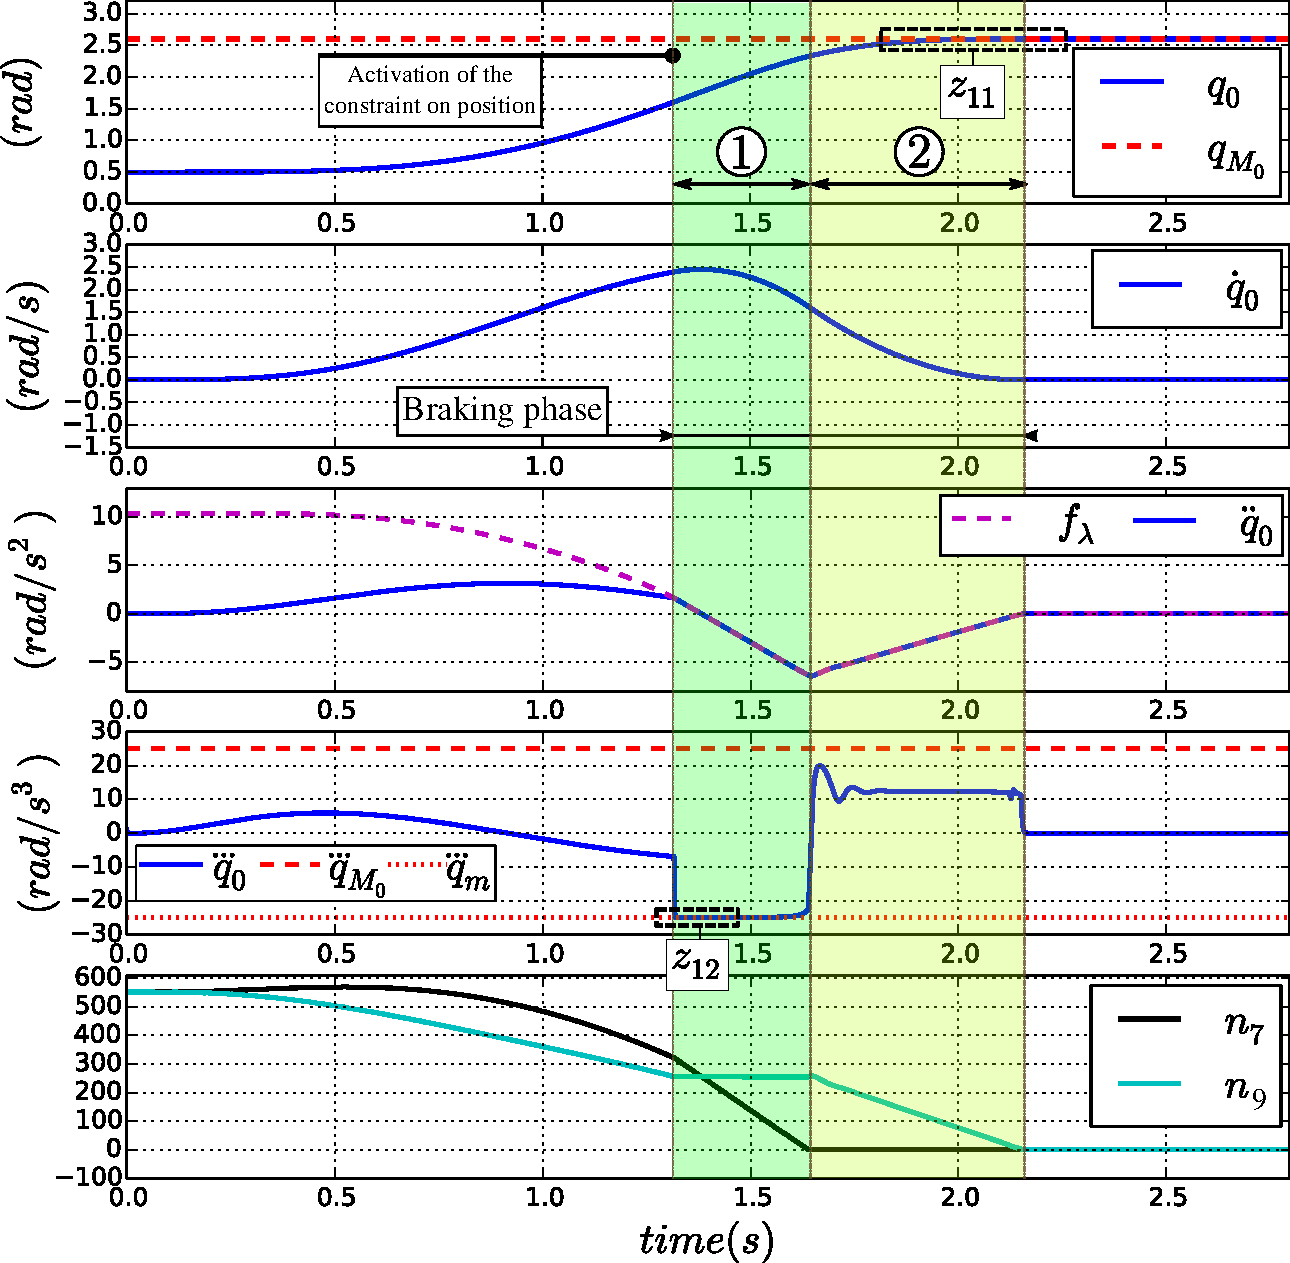
\includegraphics[width=0.8\columnwidth]{/home/anis/Desktop/THESIS_ANIS/THESIS/figures/Constrcomp/8_Posi_constr_jerk_comp_25_complete_formula_no_backklash}}
%\caption{State $S$ of joint $0$ during the braking phase to cope with a maximum position limit $q_{M_{0}}$; The new constraint formulation (\ref{eq:q_constr_on_q_ddot_with_const_qdddot_m_const_qdddot_M_1}) that takes into account both positive and negative jerk capabilities $[\dddot{q}_{m_{0}}, \dddot{q}_{M_{0}}] = [-25, 25]~rad.s^{-3}$ is used. Top to bottom: position, velocity, acceleration, jerk and ($n_7$, $n_9$).} 
%\label{fig:8_Posi_constr_jerk_comp_25_complete_formula_no_backklash}
%\end{figure}
%\begin{figure}[!htbp]
%\centering
%{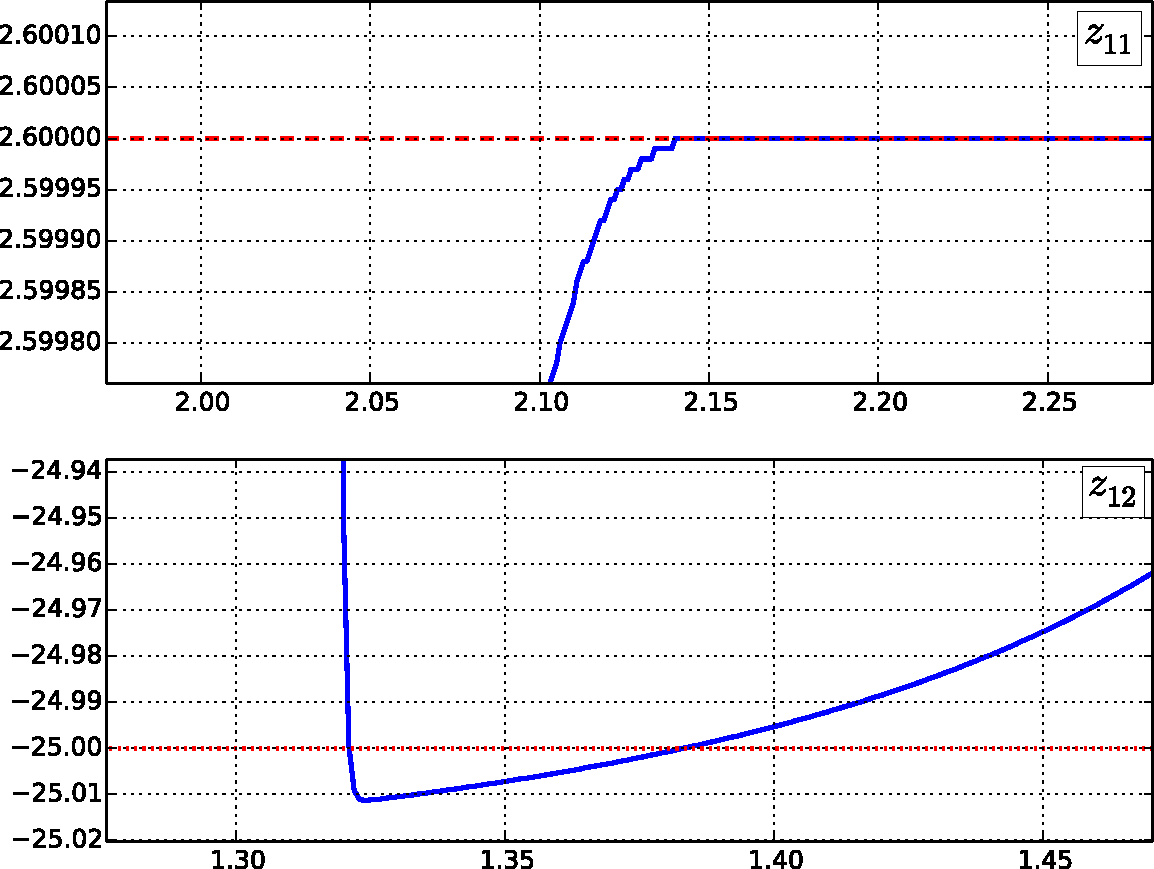
\includegraphics[width=0.8\columnwidth]{/home/anis/Desktop/THESIS_ANIS/THESIS/figures/Constrcomp/8_Posi_constr_jerk_comp_25_complete_formula_no_backklash_zoom}}
%\caption{Zooms corresponding to Fig.~\ref{fig:8_Posi_constr_jerk_comp_25_complete_formula_no_backklash}.} 
%\label{fig:8_Posi_constr_jerk_comp_25_complete_formula_no_backklash_zoom}
%\end{figure}
%
\begin{figure}[!htbp]
\centering
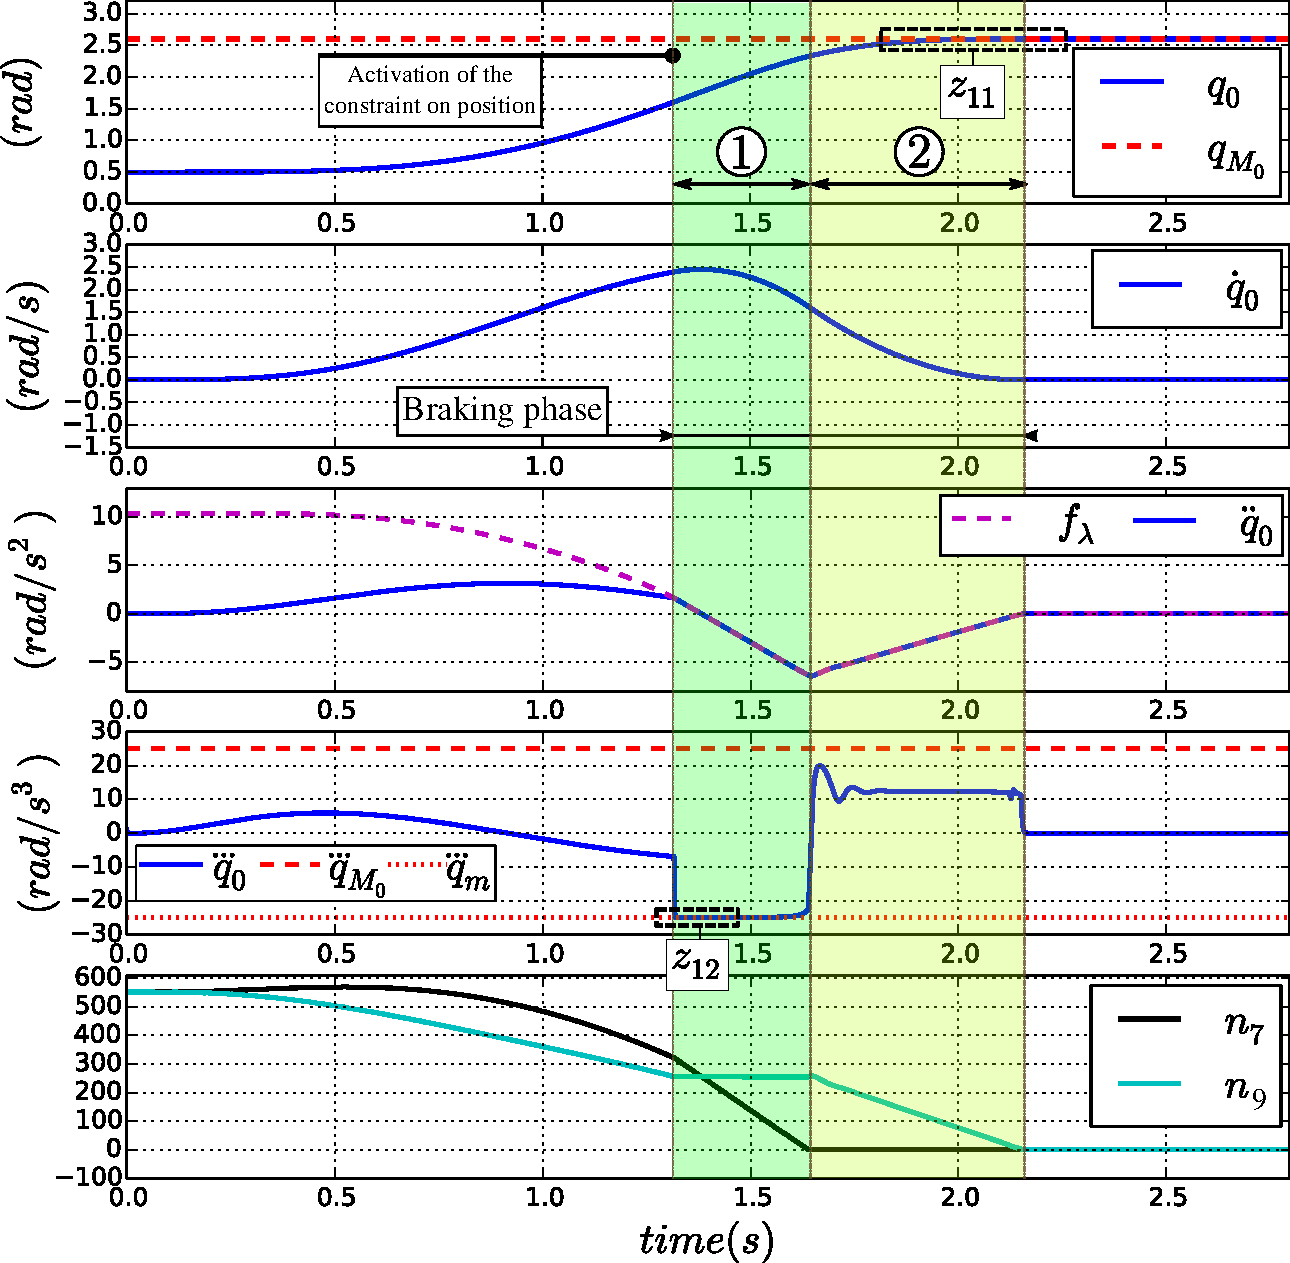
\includegraphics[width=0.99\columnwidth]{/home/anis/Desktop/THESIS_ANIS/THESIS/figures/Constrcomp/8_Posi_constr_jerk_comp_25_complete_formula_no_backklash}
\caption{Extended state $S$ of joint $0$ during the braking phase implicitly induced to cope with an upper position limit $q_{M_{0}}$. The new formulation of the constraint on articular position (\ref{eq:q_constr_on_q_ddot_with_const_qdddot_m_const_qdddot_M_1}) that takes into account both the positive and negative jerk capabilities $[\dddot{q}_{m_{0}}, \dddot{q}_{M_{0}}] = [-25, 25]~rad.s^{-3}$ is used. Top to bottom: position, velocity, acceleration, jerk and ($n_7$, $n_9$). See $z_{10}$ and $z_{11}$ in Fig.~\ref{fig:8_Posi_constr_jerk_comp_25_complete_formula_no_backklash_zoom}.} 
\label{fig:8_Posi_constr_jerk_comp_25_complete_formula_no_backklash}
\end{figure}
\begin{figure}[!htbp]
\centering
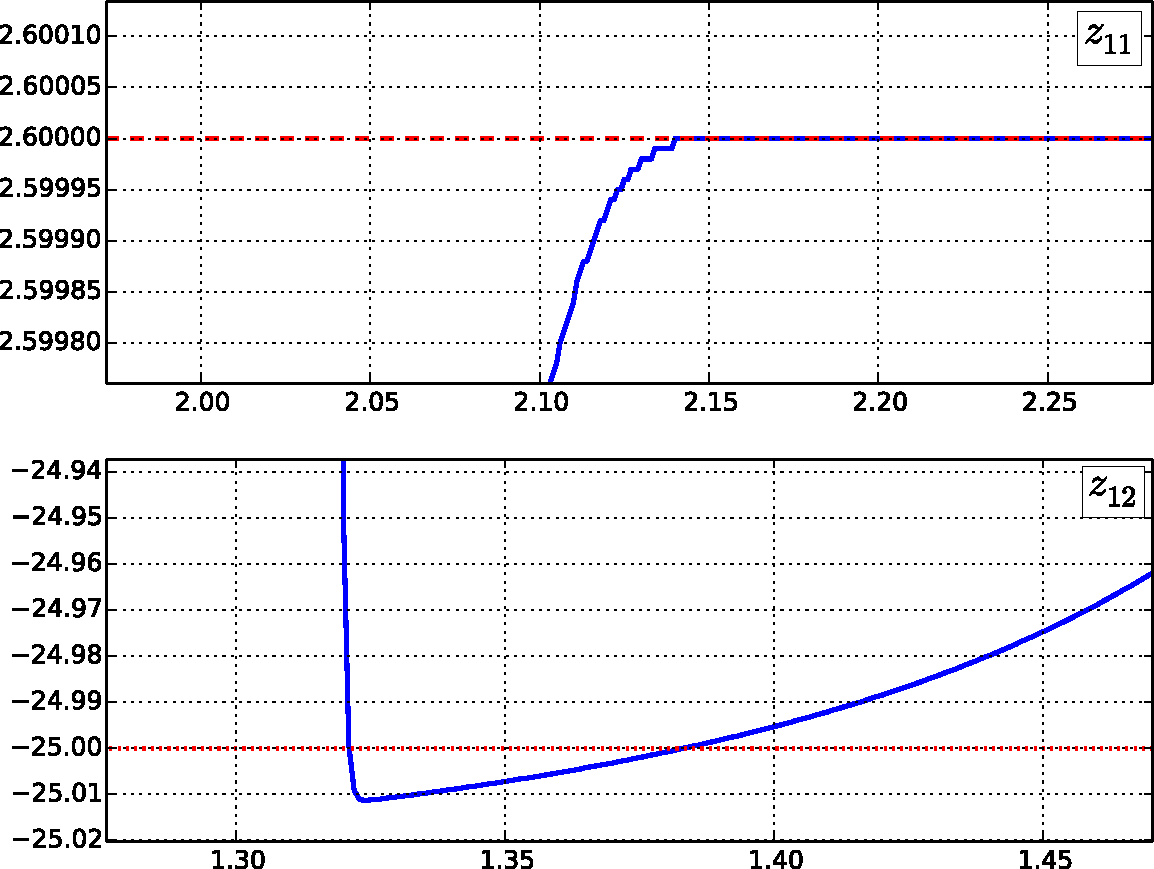
\includegraphics[width=0.90\columnwidth]{/home/anis/Desktop/THESIS_ANIS/THESIS/figures/Constrcomp/8_Posi_constr_jerk_comp_25_complete_formula_no_backklash_zoom}
\caption{Zooms corresponding to Fig.~\ref{fig:8_Posi_constr_jerk_comp_25_complete_formula_no_backklash}.} 
\label{fig:8_Posi_constr_jerk_comp_25_complete_formula_no_backklash_zoom}
\end{figure}
%
%\begin{landscape}
%\begin{figure}
%\begin{minipage}[c]{0.5\linewidth}
%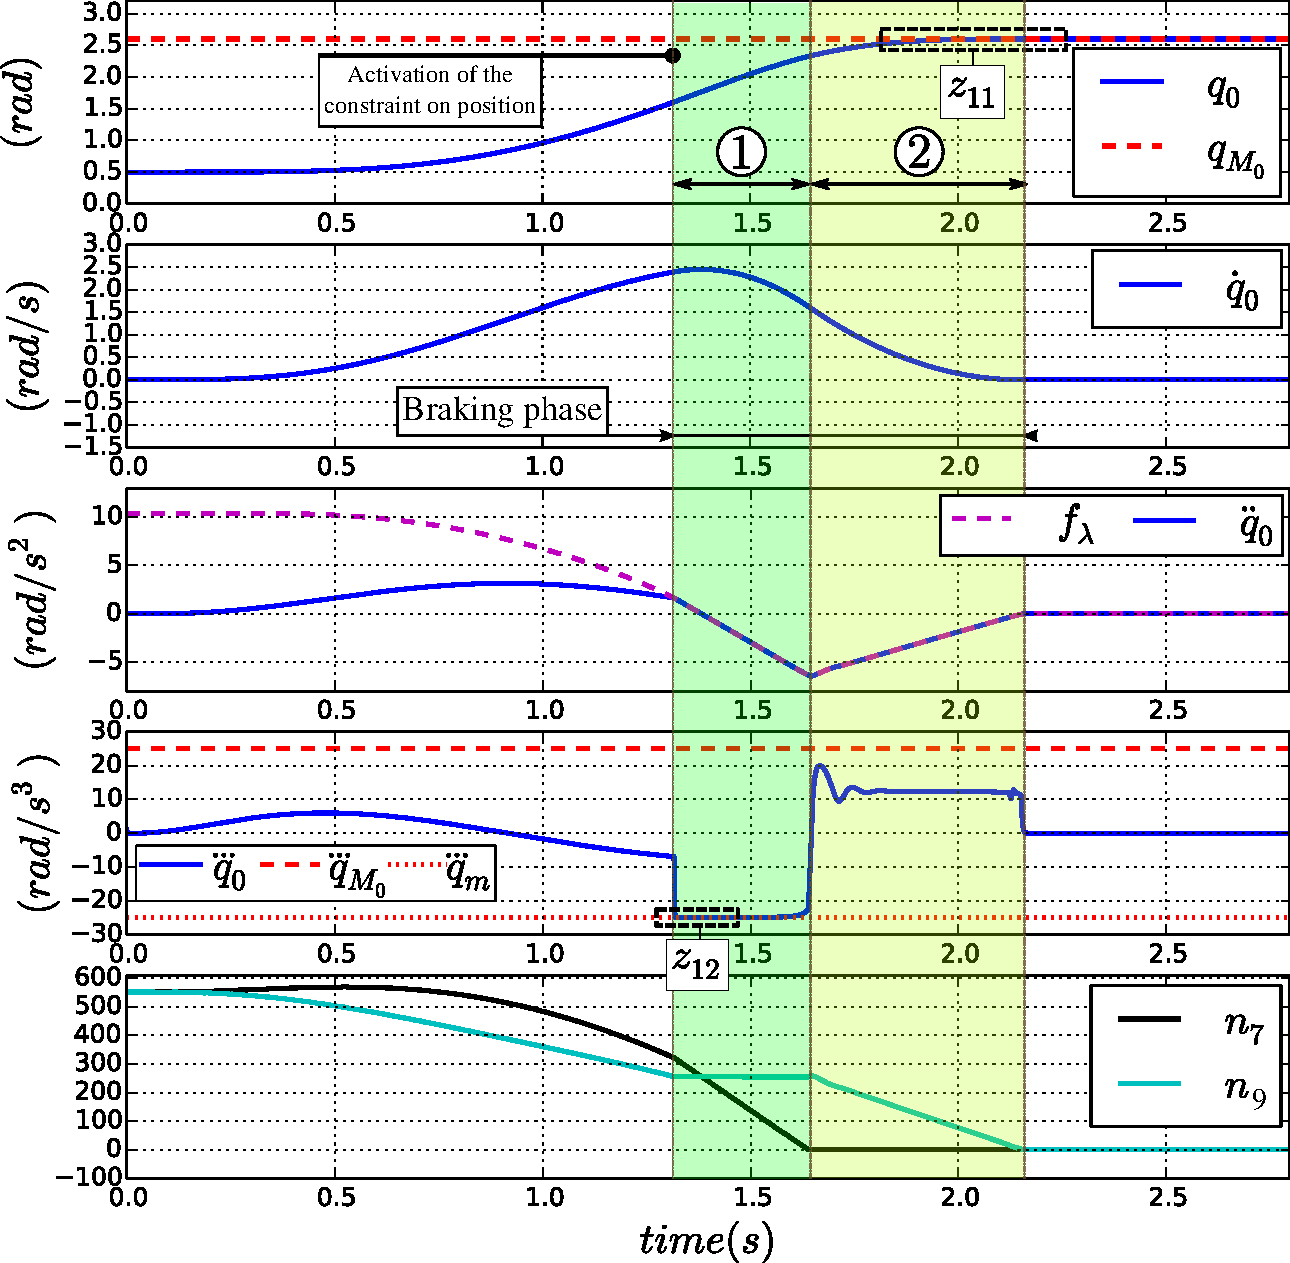
\includegraphics[width=0.99\columnwidth]{/home/anis/Desktop/THESIS_ANIS/THESIS/figures/Constrcomp/8_Posi_constr_jerk_comp_25_complete_formula_no_backklash}
%\caption{Extended state $S$ of joint $0$ during the braking phase implicitly induced to cope with an upper position limit $q_{M_{0}}$. The new formulation of the constraint on articular position (\ref{eq:q_constr_on_q_ddot_with_const_qdddot_m_const_qdddot_M_1}) that takes into account both the positive and negative jerk capabilities $[\dddot{q}_{m_{0}}, \dddot{q}_{M_{0}}] = [-25, 25]~rad.s^{-3}$ is used. Top to bottom: position, velocity, acceleration, jerk and ($n_7$, $n_9$).} 
%\label{fig:8_Posi_constr_jerk_comp_25_complete_formula_no_backklash}
%\end{minipage}
%\hfill
%\begin{minipage}[c]{0.5\linewidth}
%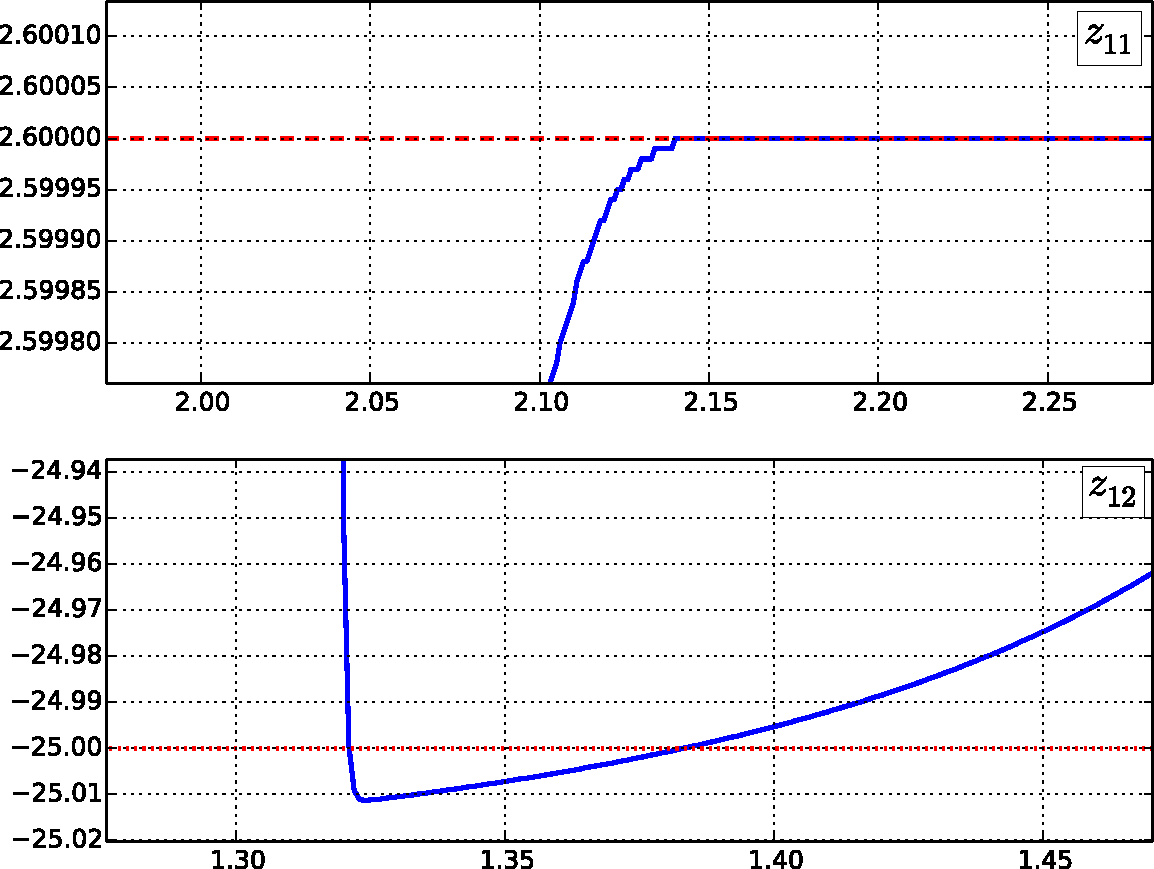
\includegraphics[width=0.90\columnwidth]{/home/anis/Desktop/THESIS_ANIS/THESIS/figures/Constrcomp/8_Posi_constr_jerk_comp_25_complete_formula_no_backklash_zoom}
%\caption{Zooms corresponding to Fig.~\ref{fig:8_Posi_constr_jerk_comp_25_complete_formula_no_backklash}.} 
%\label{fig:8_Posi_constr_jerk_comp_25_complete_formula_no_backklash_zoom}
%\end{minipage}%
%\end{figure}
%\end{landscape}
%%%%%%%%%%%%%%%%%%%%%%%%%%SUBSUBSECTION%%%%%%%%%%%%%%%%%%%%%%%%%%%%%
%%%%%%%%%%%%%%%%%%%%%%%%%%SUBSUBSECTION%%%%%%%%%%%%%%%%%%%%%%%%%%%%%
\subsubsection{Joint position constraint incompatibility with both deceleration and jerk limits 1}
\label{subsec:case4}
In all the previously introduced new formulations, the articular jerk and deceleration capabilities have been independently considered for the different mathematical expressions of the constraint on articular position. As explained in Section~\ref{subsec:complete_b_ph} regarding the description of the \nameref{label:complete} braking phase needed to \textit{\textbf{properly}} cope with an articular position limit, these capabilities $(\ddot{q}_m, \dddot{q}_m, \dddot{q}_M)$, considering an upper position limit $q_M$, should all appear together in the expression of the constraint on articular position. During the needed braking phase, the joint starts jerking negatively with maximum producible jerk $\dddot{q}_m$ during $n_{11}$ iterations. If maximum deceleration $\ddot{q}_m$ is reached, the joint brings its articular jerk to $0$ and the ``\textit{charged}'' deceleration $(\dddot{q} = \dddot{q}_m)$ is applied for $n_{13}$ iterations. Finally, the amount of deceleration in the joint is ``\textit{de-charged}'' and released during several time-steps by jerking positively towards the position limit. \\
In the following example, for \textbf{pedagogical} reasons, the braking phase to cope with an upper position limit is considered without the \textit{deceleration de-charging} sub-phase (phase \circled{3} in Fig.~\ref{fig:per_Pr_jerk_ala_3}). The \nameref{label:complete} braking phase  described hereby will be used for the final and complete formulation of the articular position constraint. The extended state \textit{S} of the system during the $(n_{11}+n_{13})$ iterations corresponding to this \textbf{truncated} ``\nameref{label:complete} braking phase'' can be described as: 
\clearpage
\begin{equation} 
\resizebox{0.81\hsize}{!}{$
\begin{split}
\left.\begin{aligned}
\textit{S}_{|k+1}&\left\{\begin{array}{lcl}
q_{|k+1} \hspace{16mm}= q_{|k} + \dot{q}_{|k} \delta t, \\
\dot{q}_{|k+1} \hspace{16mm}= \dot{q}_{|k} + \ddot{q}_{|k} \delta t, \\
\ddot{q}_{|k+1} \hspace{16mm}= \ddot{q}_{|k} + \dddot{q}_{m} \delta t;
\end{array}\right. \\
&\hspace{7mm}\vdots\ \hspace{27mm}\vdots\ \\
\textit{S}_{|k+n_{11}}&\left\{\begin{array}{lcl}
q_{|k+n_{11}} \hspace{13mm}= q_{|k+n_{11}-1} + \dot{q}_{|k+n_{11}-1} \delta t, \\
\dot{q}_{|k+n_{11}} \hspace{13mm}= \dot{q}_{|k+n_{11}-1} + \ddot{q}_{|k+n_{11}-1} \delta t, \\
\ddot{q}_{|k+n_{11}} \hspace{13mm}= \ddot{q}_{|k+n_{11}-1} + \dddot{q}_{m} \delta t;
\end{array}\right.
\end{aligned}  \hspace{27mm}\right\}\textnormal{Equivalent to (\ref{eq:discretized_dynamics_posi_jerk_braking})}  \\[0.5cm]
\left.\begin{aligned}
\textit{S}_{|k+n_{11}+1}&\left\{\begin{array}{lcl}
q_{|k+n_{11}+1}  \hspace{10mm}= q_{|k+n_{11}} + \dot{q}_{|k+n_{11}} \delta t, \\
\dot{q}_{|k+n_{11}+1}  \hspace{10mm}= \dot{q}_{|k+n_{11}} + \ddot{q}_{m} \delta t; \\
\end{array}\right.\\
&\hspace{7mm}\vdots\ \hspace{28mm}\vdots\ \\
\textit{S}_{|k+n_{11}+n_{13}}&\left\{\begin{array}{lcl}
q_{|k+n_{11}+n_{13}} \hspace{7mm}= q_{|k+n_{11}+n_{13}-1} + \dot{q}_{|k+n_{11}+n_{13}-1} \delta t, \\
\dot{q}_{|k+n_{11}+n_{13}} \hspace{7mm}= \dot{q}_{|k+n_{11}+n_{13}-1} + \ddot{q}_{m} \delta t. \\
\end{array}\right. 
\end{aligned} \hspace{13mm}\right\}\textnormal{Equivalent to (\ref{eq:discretized_dynamics_posi_decel})}  \\[0.5cm]
\end{split}$}
\label{eq:q_evolution_with_const_qdddot_m_const_const_qdddot_M}
\end{equation} 
The evolution of the joint's articular position in $(n_{11}+n_{13})$ iterations is equal to the general form\footnote{Computed using Maple \cite{maple}.} of the numerical sequence (\ref{eq:q_evolution_with_const_qdddot_m_const_const_qdddot_M}):
\begin{equation}
\begin{split}
q_{|k+n_{11}+n_{13}}=q_{|k+n_{11}} + n_{13} \dot{q}_{|k+n_{11}} \delta t + \frac{\left(n_{13}^2-n_{13}\right)}{2} \ddot{q}_m \delta t^2,
\label{eq:q_evolution_with_const_qddot_m_and_qdddot_m_final}
\end{split}
\end{equation} 
with $q_{|k+n_{11}}$ and $\dot{q}_{k+n_{11}}$, respectively equivalent to (\ref{eq:q_evolution_with_const_qdddot_m}) and   (\ref{eq:q_dot_evolution_with_const_qdddot_m}). When developed,
(\ref{eq:q_evolution_with_const_qddot_m_and_qdddot_m_final}) is written: 
\begin{equation}
\begin{split}
q_{|k+n_{11}+n_{13}} = q_{|k} &+ \left(n_{11}+n_{13}\right) \dot{q}_{|k} \delta t \\
& + \left(\frac{n_{11}^2-n_{11}}{2}+n_{11} n_{13}\right) \ddot{q}_{|k} \delta t^2 \\
& + \left[\left(\frac{n_{11}^3}{6}-\frac{n_{11}^2}{2}+\frac{n_{11}}{3})+\frac{n_{13} \left(n_{11}^2-n_{11}\right)}{2}\right] \dddot{q}_m \delta t^3 \\    
& + \frac{\left(n_{13}^2-n_{13}\right)}{2} \ddot{q}_m \delta t^2,              
\label{eq:q_evolution_with_const_qddot_m_and_qdddot_m_2_final}
\end{split}
\end{equation} 
with: $q_{|k} \geq 0$, $\dot{q}_{|k} \geq 0$ , $\dddot{q}_m \leq 0$ and $\ddot{q}_m \leq 0$. The condition $q_{|k+n_{11}+n_{13}} \leq q_M$ for all integers ($n_{11}$, $n_{13}$) in case of a control at the dynamic-level leads to:
\begin{equation}
\begin{split}
\ddot{q}_{|k}^{c} \leq &\frac{\left(q_M - q_{|k}\right)}{\left(\frac{n_{11}^2 - n_{11}}{2} + n_{11} n_{13}\right)\delta t^2} - \frac{\left(n_{11}+n_{13}\right)}{\left(\frac{n_{11}^2 - n_{11}}{2} + n_{11} n_{13}\right) \delta t} \dot{q}_{|k}\\
& -\frac{\left[\frac{n_{11}^3}{6} - \frac{n_{11}^2}{2} + \frac{n_{11}}{3} + \frac{n_{13} \left(n_{11}^2-n_{11}\right)}{2}\right]}{\left(\frac{n_{11}^2 - n_{11}}{2} + n_{11} n_{13}\right)} \dddot{q}_m \delta t \\
& - \frac{\left(n_{13}^2-n_{13}\right)}{\left(n_{11}^2 - n_{11} + 2 n_{11} n_{13}\right)}  \ddot{q}_m. 
\label{eq:Constr_comp_posi_acc_jerk_1_final}
\end{split}
\end{equation}
In case the control is performed at the kinematic-level, the constraint can be reflected on kinematic-control input $\dot{q}_{|k}^{c}$ as: 
\begin{equation}
\begin{split}
\dot{q}_{|k}^{c}  \leq &\frac{\left(q_M - q_{|k}\right)}{\left(n_{11} + n_{13}\right) \delta t}  -\frac{\left[\frac{\left(n_{11}^2-n_{11}\right)}{2} + n_{11} n_{13}\right]}{\left(n_{11} + n_{13}\right)}  \ddot{q}_{|k} \delta t\\ 
& - \frac{\left[\frac{n_{11}^3}{6} + \frac{n_{11}^2}{2} + \frac{n_{11}}{3} + \frac{n_{13} \left(n_{11}^2 - n_{11}\right)}{2}\right]}{\left(n_{11} + n_{13}\right)} \dddot{q}_m \delta t^2 \\
& - \frac{\left(n_{13}^2-n_{13}\right)}{2\left(n_{11} + n_{13}\right)} \ddot{q}_m \delta t, 
\label{eq:Constr_comp_posi_acc_jerk_1_kinema_final}
\end{split}
\end{equation}
with ($n_{11}$, $n_{13}$), the two integers minimizing the right-hand side of (\ref{eq:Constr_comp_posi_acc_jerk_1_final}).
Following the same reasoning for the lower position limit,  for all integers ($n_{12}, n_{14}$), the constraint $q_{|k+n_{12}+n_{14}} \geq q_m$ can be reflected on the acceleration control variable as: 
\begin{equation}
\begin{split}
\ddot{q}_{|k}^{c}  \geq &\frac{\left(q_m - q_{|k}\right)}{\left(\frac{n_{12}^2 - n_{12}}{2} + n_{12} n_{14}\right)\delta t^2} \\ 
& -\frac{\left[\frac{n_{12}^3}{6} - \frac{n_{12}^2}{2} + \frac{n_{12}}{3} + \frac{n_{14}\left(n_{12}^2-n_{12}\right)}{2}\right]}{\left(\frac{n_{12}^2 - n_{12}}{2} + n_{12} n_{14}\right)} \dddot{q}_M \delta t \\
& - \frac{\left(n_{12}+n_{14}\right)}{\left(\frac{n_{12}^2 - n_{12}}{2} + n_{12} n_{14}\right) \delta t} \dot{q}_{|k} - \frac{\left(n_{14}^2-n_{14}\right)}{\left(n_{12}^2 - n_{12} + 2 n_{12} n_{14}\right)}  \ddot{q}_M, 
\label{eq:Constr_comp_posi_acc_jerk_2_final}
\end{split}
\end{equation}
with $(n_{12}, n_{14})$ , the two integers maximizing the right-hand side of (\ref{eq:Constr_comp_posi_acc_jerk_2_final}). \\
$\textit{f}_{\rho}$ and $\textit{f}_{\pi}$ are respectively equivalent to the right-hand sides of (\ref{eq:Constr_comp_posi_acc_jerk_1_final}) and (\ref{eq:Constr_comp_posi_acc_jerk_2_final}). \\
%f_{\rho}(n_{12}, n_{14}), f_{\pi}(n_{11}, n_{13})$
%      n1_pos  n2_pos          n1_neg  n2_neg
%f_{{\rho}_{max}}          f_{{\pi}_{min}}
\noindent\begin{minipage}{\textwidth}
\renewcommand\footnoterule{}                  %% This line should come here.
\begin{algorithm}[H]
\caption{Compute $n_{11}, n_{12}, n_{13}, n_{14}, f_{\rho}$ and $f_{\pi}$}
\label{alg:compute_n_11_n_12_n_13_n_14_f_rho_f_pi}
\begin{algorithmic}[1]
\Require $q_M, q_m, q_{|k}, \ddot{q}_{|k},\ddot{q}_{M},\ddot{q}_{m},\dddot{q}_{M},\dddot{q}_{m}, \delta t$
\myState{$f_{{\rho}_{max}} \hspace{1mm}\gets \ddot{q}_{m}$}
\myState{$f_{{\pi}_{min}} \gets \ddot{q}_{M}$}
\For{($i_1 = 3 \rightarrow N_1$)}
\myState{$n_{11}^{*} \gets 3$}
\myState{$n_{12}^{*} \gets 3$}
\For{($i_2 = 1 \rightarrow N_2$)}
\myState{$n_{13}^{*} \hspace{1.6mm}\gets i_2$}
\myState{$n_{14}^{*} \hspace{1.6mm}\gets i_2$}
\myState{$f_{\rho}^{*} \hspace{3.5mm}\gets f_{\rho}(q_m, q_{|k}, \ddot{q}_{|k}, \dddot{q}_M, \ddot{q}_M, n_{12}^{*}, n_{14}^{*})$}
\myState{$f_{\pi}^{*} \hspace{3.6mm}\gets f_{\pi}(q_M, q_{|k}, \ddot{q}_{|k}, \dddot{q}_m, \ddot{q}_m, n_{11}^{*}, n_{13}^{*})$}
\If{($f_{\rho}^{*} \geq f_{{\rho}_{max}}$)}
\myState{$f_{{\rho}_{max}}  \gets f_{\rho}^{*}$}
\myState{$n_{12} \hspace{3.8mm}\gets n_{12}^{*}$}
\myState{$n_{14} \hspace{3.8mm}\gets n_{14}^{*}$}
\EndIf  
\If{($f_{\pi}^{*} \leq f_{{\pi}_{min}}$)}
\myState{$f_{{\pi}_{min}} \gets f_{\pi}^{*}$}
\myState{$n_{11} \hspace{3.5mm}\gets n_{11}^{*}$}
\myState{$n_{13} \hspace{3.5mm}\gets n_{13}^{*}$}
\EndIf 
\EndFor
\EndFor
\myState{$f_{\rho}  \hspace{1.5mm}\gets f_{{\rho}_{max}}$}
\myState{$f_{\pi}  \gets f_{{\pi}_{min}}$}
\myState \Return{$n_{11}, n_{12}, n_{13}, n_{14}, f_{\rho}, f_{\pi}$}\;
\end{algorithmic}
\end{algorithm}
\end{minipage} \\
\\
$n_{11}, n_{13}, n_{12}, n_{14}, f_{\rho}$ and $f_{\pi}$ can be computed numerically as shown by Algorithm~\ref{alg:compute_n_11_n_12_n_13_n_14_f_rho_f_pi}. $N_1$ and $N_2$ in Algorithm~\ref{alg:compute_n_11_n_12_n_13_n_14_f_rho_f_pi} are fixed heuristically, they must however be $\geq$ to the number of iterations needed to perform the braking movement described in (\ref{eq:q_evolution_with_const_qdddot_m_const_const_qdddot_M}). More details on how to compute this parameter in Section~\ref{sec:concl_comp_cnstr}.
%********************************************************************%
\paragraph{Illustration 5}
To illustrate the behaviour of the robot using this new theoretical result, the controller is implemented with the new version of the formulation of the constraint on articular position (\ref{eq:Constr_comp_posi_acc_jerk_1_final}), that takes into account both the articular jerk $(\dddot{q}_{m_{0}} = -25~rad.s^{-3})$ and the producible articular deceleration $\ddot{q}_{m_{0}}$. In Fig.~\ref{fig:6_Posi_constr_jerk_comp_25_non_complete_formula_backklash}, the amplitude of  the first oscillation of the joint's articular acceleration reaches $-10~rad.s^{-2}$. To demonstrate the interest of using the new formulation of the position constraint, $\ddot{q}_{m_{0}}$ is fixed at $-3~rad.s^{-2}$. The same movement of joint $0$ moving towards its upper position limit $q_{M_{0}}$ is considered; and no constraint on the articular jerk (\ref{eq:cnt_lit_tme_step_4}) is included in the configuration of the controller.  

Fig.~\ref{fig:9_Posi_constr_jerk_acc_comp_non_complete_formula_3} illustrates how joint $0$ starts braking with maximum negative jerk $(\dddot{q}_{0} = \dddot{q}_{m_{0}})$ (sub-phase \circled{1}) until maximum deceleration $(\ddot{q}_{0} = \ddot{q}_{m_{0}})$ is reached. This deceleration is then used to stop the joint at its upper position limit $q_{M_{0}}$ (sub-phase \circled{2}). As the articular jerk is not constrained, the amount of deceleration \textit{loaded} in the joint is almost instantaneously ``\textit{de-charged}'', inducing a high peak of jerk. Otherwise, if the constraint on articular jerk (\ref{eq:cnt_lit_tme_step_4}) are included in the configuration of the controller, decaying oscillations would appear as in Fig.~\ref{fig:6_Posi_constr_jerk_comp_25_non_complete_formula_backklash}. We also underline an exceeding of $(0.013~rad.s^{-3})$ over the lower jerk limit $\dddot{q}_{m_{0}}$. On the other hand, the deceleration limit $\ddot{q}_{m_{0}}$ is well satisfied (see Fig.~\ref{fig:9_Posi_constr_jerk_acc_comp_non_complete_formula_3}).
%9
%\begin{figure}[!htbp]
%\centering
%{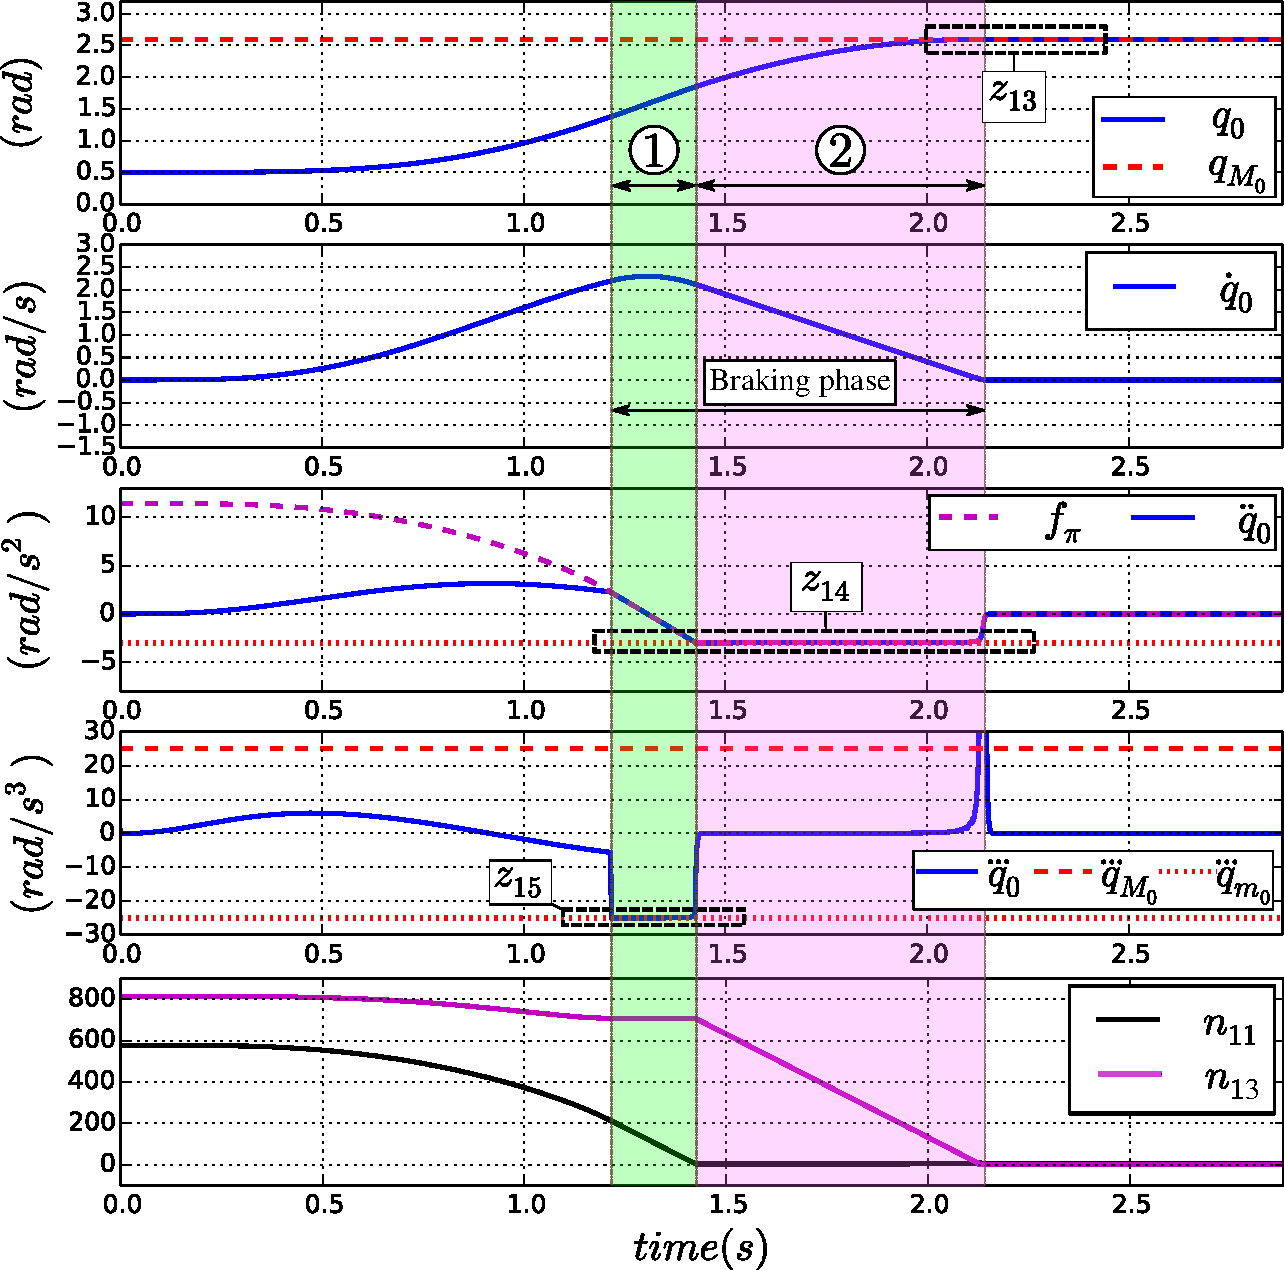
\includegraphics[width=0.8\columnwidth]{/home/anis/Desktop/THESIS_ANIS/THESIS/figures/Constrcomp/9_Posi_constr_jerk_acc_comp_non_complete_formula_3}}
%\caption{State $S$ of joint $0$ during the braking phase to cope with a maximum position limit $q_{M_{0}}$; The new constraint formulation (\ref{eq:Constr_comp_posi_acc_jerk_1_final}) that takes into account both deceleration and jerk capabilities $\dddot{q}_{m_{0}} = -25~rad.s^{-3}, \ddot{q}_{m_{0}}= -3~rad.s^{-2}$ is used. Top to bottom: position, velocity, acceleration, jerk and $(n_{11}, n_{13})$} 
%\label{fig:9_Posi_constr_jerk_acc_comp_non_complete_formula_3}
%\end{figure}
%\begin{figure}[!htbp]
%\centering
%{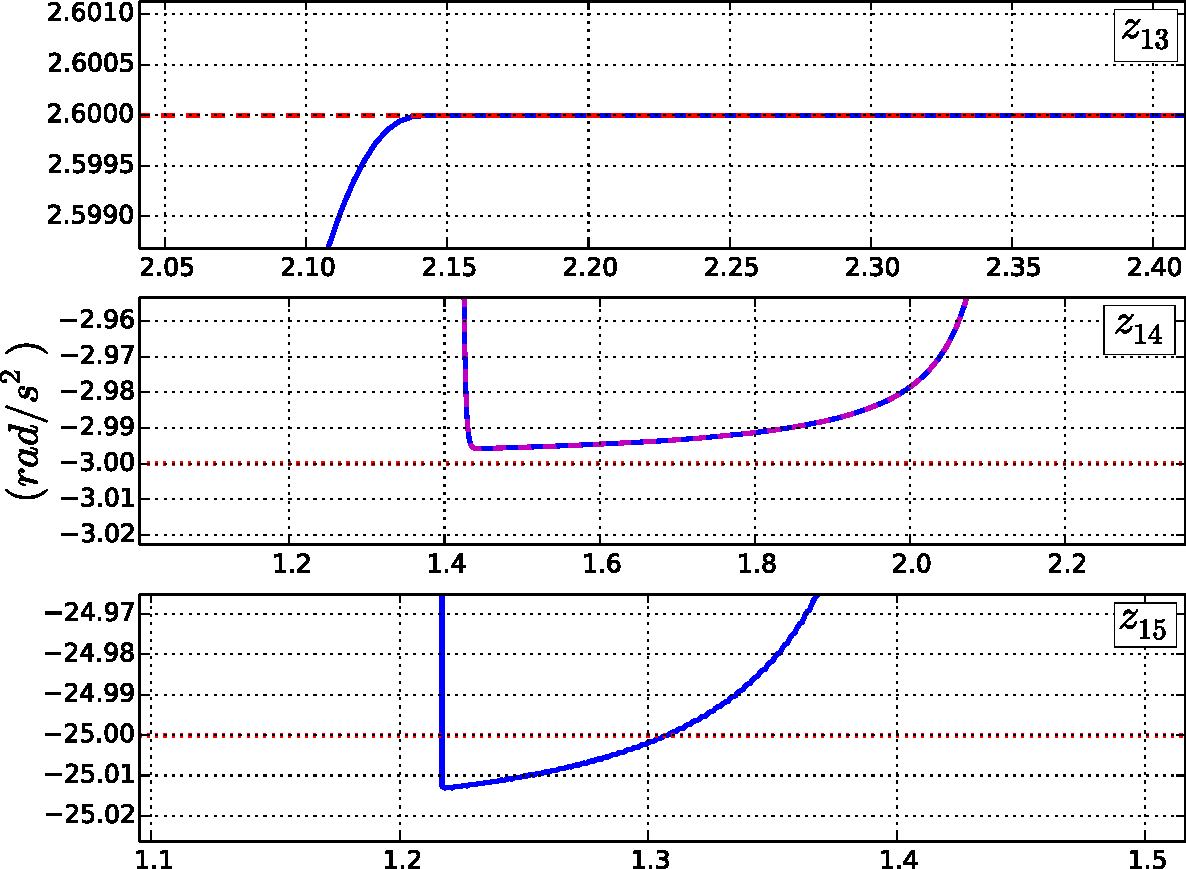
\includegraphics[width=0.8\columnwidth]{/home/anis/Desktop/THESIS_ANIS/THESIS/figures/Constrcomp/9_Posi_constr_jerk_acc_comp_non_complete_formula_3_zoom}}
%\caption{Zooms corresponding to Fig.~\ref{fig:9_Posi_constr_jerk_acc_comp_non_complete_formula_3}.} 
%\label{fig:9_Posi_constr_jerk_acc_comp_non_complete_formula_3_zoom}
%\end{figure}
\begin{figure}[!htbp]
\centering
\includegraphics[width=0.92\columnwidth]{/home/anis/Desktop/THESIS_ANIS/THESIS/figures/Constrcomp/9_Posi_constr_jerk_acc_comp_non_complete_formula_3}
\caption{Extended state $S$ of joint $0$ during a \textit{non-complete} braking phase implicitly induced to cope with an upper position limit $q_{M_{0}}$. The new formulation of the constraint on articular position (\ref{eq:Constr_comp_posi_acc_jerk_1_final}), that takes into account both the articular jerk and deceleration capabilities $(\dddot{q}_{m_{0}} = -25~rad.s^{-3})$, $(\ddot{q}_{m_{0}}= -3~rad.s^{-2})$ is used. Top to bottom: position, velocity, acceleration, jerk and $(n_{11}, n_{13})$. See $z_{13}$ and $z_{14}$ in Fig.~\ref{fig:9_Posi_constr_jerk_acc_comp_non_complete_formula_3_zoom}.} 
\label{fig:9_Posi_constr_jerk_acc_comp_non_complete_formula_3}
\end{figure}
\begin{figure}[!htbp]
\centering
\includegraphics[width=0.90\columnwidth]{/home/anis/Desktop/THESIS_ANIS/THESIS/figures/Constrcomp/9_Posi_constr_jerk_acc_comp_non_complete_formula_3_zoom}
\caption{Zooms corresponding to Fig.~\ref{fig:9_Posi_constr_jerk_acc_comp_non_complete_formula_3}.} 
\label{fig:9_Posi_constr_jerk_acc_comp_non_complete_formula_3_zoom}
\end{figure}
%
%\begin{landscape}
%\begin{figure}
%\begin{minipage}[c]{0.5\linewidth}
%\includegraphics[width=0.99\columnwidth]{/home/anis/Desktop/THESIS_ANIS/THESIS/figures/Constrcomp/9_Posi_constr_jerk_acc_comp_non_complete_formula_3}
%\caption{Extended state $S$ of joint $0$ during a \textit{non-complete} braking phase implicitly induced to cope with an upper position limit $q_{M_{0}}$. The new formulation of the constraint on articular position (\ref{eq:Constr_comp_posi_acc_jerk_1_final}), that takes into account both the articular jerk and deceleration capabilities $(\dddot{q}_{m_{0}} = -25~rad.s^{-3})$, $(\ddot{q}_{m_{0}}= -3~rad.s^{-2})$ is used. Top to bottom: position, velocity, acceleration, jerk and $(n_{11}, n_{13})$} 
%\label{fig:9_Posi_constr_jerk_acc_comp_non_complete_formula_3}
%\end{minipage}
%\hfill
%\begin{minipage}[c]{0.5\linewidth}
%\includegraphics[width=0.90\columnwidth]{/home/anis/Desktop/THESIS_ANIS/THESIS/figures/Constrcomp/9_Posi_constr_jerk_acc_comp_non_complete_formula_3_zoom}
%\caption{Zooms corresponding to Fig.~\ref{fig:9_Posi_constr_jerk_acc_comp_non_complete_formula_3}.} 
%\label{fig:9_Posi_constr_jerk_acc_comp_non_complete_formula_3_zoom}
%\end{minipage}%
%\end{figure}
%\end{landscape}
%%%%%%%%%%%%%%%%%%%%%%%%%%SUBSUBSECTION%%%%%%%%%%%%%%%%%%%%%%%%%%%%%
%%%%%%%%%%%%%%%%%%%%%%%%%%SUBSUBSECTION%%%%%%%%%%%%%%%%%%%%%%%%%%%%%
\subsubsection{Joint position constraint incompatibility with both jerk and deceleration limits 2}
\label{subsec:case5}
Finally, the fully \nameref{label:complete} description of the braking phase is used to derive the \textit{proper} and complete formulation of the constraint on articular position. When coping with an upper position limit $q_M$, such braking phase is as follows: 1) the joint starts jerking with maximum negative jerk $\dddot{q}_{m}$ for $n_{15}$ iterations until maximum producible articular deceleration $\ddot{q}_m$ is reached. 2) This deceleration is then applied for $n_{17}$ control time-steps then, 3) ``\textit{de-charged}'' during $n_{19}$ iterations by jerking positively with maximum producible jerk $\dddot{q}_M$ (see Fig.~\ref{fig:per_Pr_jerk_ala_3}). The extended state \textit{S} of the system during this \nameref{label:complete} braking phase can be described as:  
\clearpage
\begin{equation} 
\resizebox{0.89\hsize}{!}{$
\begin{split}
\left.\begin{aligned}
\textit{S}_{|k+1}&\left\{\begin{array}{lcl}
q_{|k+1} \hspace{17mm}= q_{|k} + \dot{q}_{|k} \delta t, \\
\dot{q}_{|k+1} \hspace{17mm}= \dot{q}_{|k} + \ddot{q}_{|k} \delta t, \\
\ddot{q}_{|k+1} \hspace{17mm}= \ddot{q}_{|k} + \dddot{q}_{m} \delta t;
\end{array}\right. \\
&\hspace{7mm}\vdots\ \hspace{28mm}\vdots\ \\
\textit{S}_{|k+n_{15}}&\left\{\begin{array}{lcl}
q_{|k+n_{15}} \hspace{14mm}= q_{|k+n_{15}-1} + \dot{q}_{|k+n_{15}-1} \delta t, \\
\dot{q}_{|k+n_{15}} \hspace{14mm}= \dot{q}_{|k+n_{15}-1} + \ddot{q}_{|k+n_{15}-1} \delta t, \\
\ddot{q}_{|k+n_{15}} \hspace{14mm}= \ddot{q}_{|k+n_{15}-1} + \dddot{q}_{m} \delta t;
\end{array}\right.
\end{aligned}  \hspace{26mm}\right\}\textnormal{Equivalent to (\ref{eq:discretized_dynamics_posi_jerk_braking})}  \\[0.5cm]
\left.\begin{aligned}
\textit{S}_{|k+n_{15}+1}&\left\{\begin{array}{lcl}
q_{|k+n_{15}+1}  \hspace{10mm}= q_{|k+n_{15}} + \dot{q}_{|k+n_{15}} \delta t, \\
\dot{q}_{|k+n_{15}+1}  \hspace{10mm}= \dot{q}_{|k+n_{15}} + \ddot{q}_{m} \delta t; \\
\end{array}\right.\\
&\hspace{7mm}\vdots\ \hspace{28mm}\vdots\ \\
\textit{S}_{|k+n_{15}+n_{17}}&\left\{\begin{array}{lcl}
q_{|k+n_{15}+n_{17}} \hspace{7mm}= q_{|k+n_{15}+n_{17}-1} + \dot{q}_{|k+n_{15}+n_{17}-1} \delta t, \\
\dot{q}_{|k+n_{15}+n_{17}} \hspace{7mm}= \dot{q}_{|k+n_{15}+n_{17}-1} + \ddot{q}_{m} \delta t; \\
\end{array}\right. 
\end{aligned} \hspace{13mm}\right\}\textnormal{Equivalent to (\ref{eq:discretized_dynamics_posi_decel})}  \\[0.5cm]
\left.\begin{aligned}
\textit{S}_{|k+n_{15}+n_{17}+1}&\left\{\begin{array}{lcl}
q_{|k+n_{15}+n_{17}+1} \hspace{3mm}= q_{|k+n_{15}+n_{17}} + \dot{q}_{|k+n_{15}+n_{17}} \delta t, \\
\dot{q}_{|k+n_{15}+n_{17}+1} \hspace{3mm}= \dot{q}_{|k+n_{15}+n_{17}} + \ddot{q}_{|k+n_{15}+n_{17}} \delta t, \\
\ddot{q}_{|k+n_{15}+n_{17}+1}  \hspace{3mm}= \ddot{q}_{|k+n_{15}+n_{17}} + \dddot{q}_{M} \delta t;
\end{array}\right.\\
&\hspace{7mm}\vdots\ \hspace{29mm}\vdots\ \\
\textit{S}_{|k+n_{15}+n_{17}+n_{19}}&\left\{\begin{array}{lcl}
q_{|k+n_{15}+n_{17}+n_{19}} = q_{|k+n_{15}+n_{17}+n_{19}-1} + \dot{q}_{|k+n_{15}+n_{17}+n_{19}-1} \delta t, \\
\dot{q}_{|k+n_{15}+n_{17}+n_{19}} = \dot{q}_{|k+n_{15}+n_{17}+n_{19}-1} + \ddot{q}_{|k+n_{15}+n_{17}+n_{19}-1} \delta t, \\
\ddot{q}_{|k+n_{15}+n_{17}+n_{19}} = \ddot{q}_{|k+n_{15}+n_{17}+n_{19}-1} + \dddot{q}_{M} \delta t.
\end{array}\right.
\end{aligned}\right\}\textnormal{Equivalent to (\ref{eq:discretized_dynamics_posi_jerk_braking})} 
\end{split}$}
\label{eq:S_with_const_qdddot_m_const_qddot_m_const_qdddot_M}
\end{equation} 
The evolution of the joint's articular position in $(n_{15}+n_{17}+n_{19})$ iterations is equal to the general form\footnote{Computed using Maple \cite{maple}.} of the numerical sequence  (\ref{eq:S_with_const_qdddot_m_const_qddot_m_const_qdddot_M}):
\begin{equation}
\begin{split}
q_{|k+n_{15}+n_{17}+n_{19}} = &q_{|k+n_{15} + n_{17}} + n_{19} \dot{q}_{|k+n_{15}+n_{17}} \delta t \\
&+ \frac{\left(n_{19}^{2}-n_{19}\right)}{2} \ddot{q}_{|k+n_{15}+n_{17}} \delta t^{2} \\
&+ \left(\frac{n_{19}^{3}}{6}-\frac{n_{19}^{2}}{2}+\frac{n_{19}}{3}\right) \dddot{q}_{M} \delta t^{3},
\end{split}
\label{eq:q_evolution_with_const_qdddot_m_const_qddot_m_const_qdddot_M}
\end{equation} 
with: \\
\begin{equation}
\left\{\begin{array}{lcl}
q_{|k+n_{15}+n_{17}} = q_{|k+n_{15}} + n_{17}  \dot{q}_{|k+n_{15}} \delta t + \frac{\left(n_{17}^{2}-n_{17}\right)}{2} \ddot{q}_{m} \delta t^{2}, \\
\hspace{20mm}= q_{|k} + \left(n_{15}+n_{17}\right) \dot{q}_{|k} \delta t + \left[\left(n_{15} n_{17}\right)+\frac{\left(n_{15}^2-n_{15}\right)}{2}\right] \ddot{q}_{|k} \delta t^2 \\
\hspace{24mm}+ \frac{\left(n_{17}^2-n_{17}\right)}{2} \ddot{q}_{m} \delta t^2 \\
\hspace{24mm}+ \left[\frac{n_{17}\left(n_{15}^2-n_{15}\right)}{2}+\left(\frac{n_{15}^3}{6}-\frac{n_{15}^2}{2}+\frac{n_{15}}{3}\right)\right] \dddot{q}_{m} \delta t^3, \\
\dot{q}_{|k+n_{15}+n_{17}} = \dot{q}_{|k+n_{15}} + n_{17} \ddot{q}_{m} \delta t, \\
\hspace{20mm}= \dot{q}_{|k} + n_{15} \ddot{q}_{|k} \deta t + \frac{\left(n_{15}^{2}-n_{15}\right)}{2} \dddot{q}_{m} \delta t^{2} + n_{17} \ddot{q}_{m} \delta t, \\
\ddot{q}_{|k+n_{15}+n_{17}} \hspace{1mm}= \ddot{q}_{|k} + \dddot{q}_{m} \delta t. 
\end{array}\right. 
\end{equation}
$q_{|k+n_{15}}$, $q_{|k+n_{15}+n_{17}}$ and $\dot{q}_{|k+n_{15}}$ are respectively equivalent to  (\ref{eq:q_evolution_with_const_qdddot_m}), (\ref{eq:q_evolution_with_const_qddot_m_and_qdddot_m_2_final}) and (\ref{eq:q_dot_evolution_with_const_qdddot_m}). When developed, (\ref{eq:q_evolution_with_const_qdddot_m_const_qddot_m_const_qdddot_M}) becomes:
\begin{equation}
\begin{split}
q_{|k+n_{15}+n_{17}+n_{19}} =\hspace{1mm}&q_{|k} + \left(n_{15}+n_{17}+n_{19}\right) \dot{q}_{|k} \delta t \\
&+ \left[n_{15}\left(n_{17}+n_{19}\right)+\frac{\left(n_{15}^2-n_{15}\right)+\left(n_{19}^2-n_{19}\right)}{2}]\ddot{q}_{|k} \delta t^2 \\
&+ \left[\frac{\left(n_{17}+n_{19}\right)+\left(n_{15}^2-n_{15}\right)}{2}+\left(\frac{n_{15}^3}{6}-\frac{n_{15}^2}{2}+\frac{n_{15}}{3}\right)\right]\dddot{q}_{m} \delta t^3 \\
&+ \left[\left(n_{17} n_{19}\right)+\frac{\left(n_{17}^2-n_{17}\right)+\left(n_{19}^2-n_{19}\right)}{2}\right] \ddot{q}_{m} \delta t^2 \\
&+ \left(\frac{n_{19}^3}{6}-\frac{n_{19}^2}{2}+\frac{n_{19}}{3}\right)\dddot{q}_{M} \delta t^3.
\end{split}
\label{eq:q_evolution_with_const_qdddot_m_const_qddot_m_const_qdddot_M_dev}
\end{equation} 
With: $q_{|k} \geq 0$, $\dot{q}_{|k} \geq 0$ , $\dddot{q}_m \leq 0$, $\ddot{q}_m \leq 0$ and $\dddot{q}_M \geq 0$. The condition $q_{|k+n_{15}+n_{17}+n_{19}} \leq q_M$ for all integers $(n_{15}$, $n_{17}$, $n_{19})$ leads to:
\begin{equation}
\begin{split}
\ddot{q}_{|k}^{c} \leq &\frac{\left(q_{M}-q_{|k}\right)}{\left[n_{15}\left(n_{17}+n_{19}\right)+\frac{\left(n_{15}^2-n_{15}\right)+\left(n_{19}^2-n_{19}\right)}{2}\right]\delta t^2} \\
&- \frac{\left(n_{15}+n_{17}+n_{19}\right)\dot{q}_{|k}}{\left[n_{15}\left(n_{17}+n_{19}\right)+\frac{\left(n_{15}^2-n_{15}\right)+\left(n_{19}^2-n_{19}\right)}{2}\right]\delta t} \\
&- \frac{\left[\frac{\left(n_{17}+n_{19}\right)+\left(n_{15}^2-n_{15}\right)}{2}+\left(\frac{n_{15}^3}{6}-\frac{n_{15}^2}{2}+\frac{n_{15}}{3}\right)\right]\dddot{q}_{m} \delta t}{\left[n_{15}\left(n_{17}+n_{19}\right)+\frac{\left(n_{15}^2-n_{15}\right)+\left(n_{19}^2-n_{19}\right)}{2}\right]} \\
&- \frac{\left[\left(n_{17} n_{19}\right)+\frac{\left(n_{17}^2-n_{17}\right)+\left(n_{19}^2-n_{19}\right)}{2}\right]\ddot{q}_{m}}{\left[n_{15}\left(n_{17}+n_{19}\right)+\frac{\left(n_{15}^2-n_{15}\right)+\left(n_{19}^2-n_{19}\right)}{2}\right]} \\
&- \frac{\left[\left(\frac{n_{19}^3}{6}-\frac{n_{19}^2}{2}+\frac{n_{19}}{3}\right)\right]\dddot{q}_{M} \delta t}{\left[n_{15}\left(n_{17}+n_{19}\right)+\frac{\left(n_{15}^2-n_{15}\right)+\left(n_{19}^2-n_{19}\right)}{2}\right]}.
\end{split}
\label{eq:q_ddot_posi_acc_jerk_comp_complete_1}
\end{equation} 
$(n_{15}$, $n_{17}$, $n_{19})$ are the integers minimizing the right-hand side of (\ref{eq:q_ddot_posi_acc_jerk_comp_complete_1}).
Following the same reasoning for the lower position limit, the condition $q_{|k+n_{16}+n_{18}+n_{20}} \geq q_{m}$ can be reflected on the acceleration control variable as follows:
\begin{equation}
\begin{split}
\ddot{q}_{|k}^{c} \geq &\frac{\left(q_{m}-q_{|k}\right)}{\left[n_{16}\left(n_{18}+n_{20}\right)+\frac{\left(n_{16}^2-n_{16}\right)+\left(n_{20}^2-n_{20}\right)}{2}\right]\delta t^2} \\
&- \frac{\left(n_{16}+n_{18}+n_{20}\right)\dot{q}_{|k}}{\left[n_{16}\left(n_{18}+n_{20}\right)+\frac{\left(n_{16}^2-n_{16}\right)+\left(n_{20}^2-n_{20}\right)}{2}\right]\delta t} \\
&- \frac{\left[\frac{\left(n_{18}+n_{20}\right)+\left(n_{16}^2-n_{16}\right)}{2}+\left(\frac{n_{16}^3}{6}-\frac{n_{16}^2}{2}+\frac{n_{16}}{3}\right)\right]\dddot{q}_{M} \delta t}{\left[n_{16}\left(n_{18}+n_{20}\right)+\frac{\left(n_{16}^2-n_{16}\right)+\left(n_{20}^2-n_{20}\right)}{2}\right]} \\
&- \frac{\left[\left(n_{18} n_{20}\right)+\frac{\left(n_{18}^2-n_{18}\right)+\left(n_{20}^2-n_{20}\right)}{2}\right]\ddot{q}_{M}}{\left[n_{16}\left(n_{18}+n_{20}\right)+\frac{\left(n_{16}^2-n_{16}\right)+\left(n_{20}^2-n_{20}\right)}{2}\right]} \\
&- \frac{\left(\frac{n_{20}^3}{6}-\frac{n_{20}^2}{2}+\frac{n_{20}}{3}\right)\dddot{q}_{m} \delta t}{\left[n_{16}\left(n_{18}+n_{20}\right)+\frac{\left(n_{16}^2-n_{16}\right)+\left(n_{20}^2-n_{20}\right)}{2}\right]},
\end{split}
\label{eq:q_ddot_posi_acc_jerk_comp_complete_2}
\end{equation} 
with $(n_{16}, n_{18}, n_{20})$: the integers maximizing the right-hand side of (\ref{eq:q_ddot_posi_acc_jerk_comp_complete_2}). \\
$\textit{f}_{\chi}$ and $\textit{f}_{\phi}$ are respectively equivalent to the right-hand sides of (\ref{eq:q_ddot_posi_acc_jerk_comp_complete_1}) and (\ref{eq:q_ddot_posi_acc_jerk_comp_complete_2}). \\
\noindent\begin{minipage}{\textwidth}
\renewcommand\footnoterule{}                  %% This line should come here.
\begin{algorithm}[H]
\caption{Compute $n_{15}, n_{16}, n_{17}, n_{18}, n_{19}, n_{20}, f_{\chi}$ and $f_{\phi}$}
\label{alg:compute_n_15_n_16_n_17_n_18_n_19_n_20_f_chi_f_phi}
\begin{algorithmic}[1]
%f_{\phi}(n_{16}, n_{18}, n_{20}) and f_{\chi}(n_{15}, n_{17}, n_{19})  
      % n1_pos  n2_pos  n3_pos             n1_neg  n2_neg  n3_neg
\Require $q_M, q_m, q_{|k}, \dot{q}_{|k}, \ddot{q}_{M},\ddot{q}_{m},\dddot{q}_{M},\dddot{q}_{m}, \delta t$
\State{$f_{{\chi}_{max}} \hspace{0.5mm} \gets \ddot{q}_{m} \qquad f_{{\phi}_{min}} \hspace{0.5mm} \gets \ddot{q}_{M}$}
%\myState{$f_{{\chi}_{max}} \hspace{0.5mm} \gets \ddot{q}_{m}$}
%\myState{$f_{{\phi}_{min}} \hspace{0.5mm} \gets \ddot{q}_{M}$} 
\For{($i_1 = 1 \rightarrow N_1$)}
\State{$n_{16}^{*} \gets i_1 \qquad n_{15}^{*} \gets i_1$}
%\myState{$n_{16}^{*} \gets i_1$}
%\myState{$n_{15}^{*} \gets i_1$}
\For{($i_2 = 0 \rightarrow N_2$)}
\State{$n_{18}^{*} \gets i_2 \qquad n_{17}^{*} \gets i_2$}
%\myState{$n_{18}^{*} \gets i_2$}
%\myState{$n_{17}^{*} \gets i_2$}
        \If{($\ddot{q}_{|k} \geq 0$)} 
             \State{$n_{{20}_{\mathbb{R}^{+}}}^{*} \gets n_{16}-\abs[\Big]{\myfrac[5pt]{\ddot{q}_{|k}}{\dddot{q}_m \delta t}} \qquad n_{{19}_{\mathbb{R}^{+}}}^{*} \gets n_{15}+\abs[\Big]{\myfrac[5pt]{\ddot{q}_{|k}}{\dddot{q}_M \delta t}}$}
%             \myState{$n_{20}^{*} \gets n_{16}-\abs[\Big]{\myfrac[5pt]{\ddot{q}_{|k}}{\dddot{q}_m \delta t}}$}
%             \myState{$n_{19}^{*} \gets n_{15}+\abs[\Big]{\myfrac[5pt]{\ddot{q}_{|k}}{\dddot{q}_M \delta t}}$}
        \EndIf 
        \If{($\ddot{q}_{|k} < 0$)} 
             \State{$n_{{20}_{\mathbb{R}^{+}}}^{*} \gets n_{16}+\abs[\Big]{\myfrac[5pt]{\ddot{q}_{|k}}{\dddot{q}_M \delta t}} \qquad n_{{19}_{\mathbb{R}^{+}}}^{*} \gets n_{15}-\abs[\Big]{\myfrac[5pt]{\ddot{q}_{|k}}{\dddot{q}_m \delta t}}$}
%             \myState{$n_{20}^{*} \gets n_{16}+\abs[\Big]{\myfrac[5pt]{\ddot{q}_{|k}}{\dddot{q}_M \delta t}}$}
%             \myState{$n_{19}^{*} \gets n_{15}-\abs[\Big]{\myfrac[5pt]{\ddot{q}_{|k}}{\dddot{q}_m \delta t}}$}
%        \If{($n_{15}^{*} \leq 1$)}
%             \myState{$n_{20}^{*} \gets \abs[\Big]{\myfrac[5pt]{\ddot{q}_{|k}}{\dddot{q}_M \delta t}}$}
%        \EndIf
        \IfThenElse{($n_{16}^{*} \leq 1$)}% If ...
            {$n_{{20}_{\mathbb{R}^{+}}}^{*} \gets \abs[\Big]{\myfrac[5pt]{\ddot{q}_{|k}}{\dddot{q}_m \delta t}}$}% ...then... 
\vspace{1.5mm}             
%        \If{($n_{16}^{*} \leq 1$)}
%             \myState{$n_{19}^{*} \gets \abs[\Big]{\myfrac[5pt]{\ddot{q}_{|k}}{\dddot{q}_m \delta t}}$}
%        \EndIf
        \IfThenElse{($n_{15}^{*} \leq 1$)}% If ...
            {$n_{{19}_{\mathbb{R}^{+}}}^{*} \gets \abs[\Big]{\myfrac[5pt]{\ddot{q}_{|k}}{\dddot{q}_M \delta t}}$}% ...then...
        
        \EndIf
%f_{\phi}(n_{16}, n_{18}, n_{20}) and f_{\chi}(n_{15}, n_{17}, n_{19})  
      % n1_pos  n2_pos  n3_pos             n1_neg  n2_neg  n3_neg
\IfThenElse{($n_{15}^{*} \leq 1$)}% If ...
            {$n_{15}^{*} \gets 1$}% ...then...
\IfThenElse{($n_{16}^{*} \leq 1$)}% If ...
            {$n_{16}^{*} \gets 1$}% ...then...            
\IfThenElse{($n_{{19}_{\mathbb{R}^{+}}}^{*} \leq 2$)}% If ...
            {$n_{{19}_{\mathbb{R}^{+}}}^{*} \gets 2$}% ...then...
\IfThenElse{($n_{{20}_{\mathbb{R}^{+}}}^{*} \leq 2$)}% If ...
            {$n_{{20}_{\mathbb{R}^{+}}}^{*} \gets 2$}% ...then...      
\myState{$f_{\chi}^{*} \gets f_{\chi}(q_m, q_{|k}, \dot{q}_{|k}, \dddot{q}_M, \ddot{q}_M, \dddot{q}_m, n_{15}^{*}, n_{17}^{*}, n_{19}^{*})$}
\myState{$f_{\phi}^{*} \gets f_{\phi}(q_M, q_{|k}, \dot{q}_{|k}, \dddot{q}_m, \ddot{q}_m, \dddot{q}_M, n_{16}^{*}, n_{18}^{*}, n_{20}^{*})$}
\If{($f_{\chi}^{*} \geq f_{{\chi}_{max}}$)}
\State{$f_{{\chi}_{max}} \gets f_{\chi}^{*} \qquad n_{16} \gets n_{16}^{*} \qquad n_{18} \gets n_{18}^{*} \qquad n_{20}$\footnote{\label{note2} For stability in the computation of $f_{\chi}$ and $f_{\phi}$, ($n_{19}^{*}, n_{20}^{*}$) are used as real numbers (even if previously defined as numbers of iterations). The same for $n_{19}$ and $n_{20}$.} $\gets n_{{20}_{\mathbb{R}^{+}}}^{*}$}
%\myState{$f_{{\chi}_{max}} \gets f_{\chi}^{*}$}
%\myState{$n_{16} \gets n_{16}^{*}$}
%\myState{$n_{18} \gets n_{18}^{*}$}
%\myState{$n_{20} \gets n_{20}^{*}$}
\EndIf 
\If{($f_{\phi}^{*} \leq f_{{\phi}_{min}}$)}
\State{$f_{{\phi}_{min}} \gets f_{\phi}^{*} \qquad n_{15} \gets n_{15}^{*} \qquad n_{17} \gets n_{17}^{*} \qquad n_{19}\footnoteref{note2} \gets n_{{19}_{\mathbb{R}^{+}}}^{*}$}
%\myState{$f_{{\phi}_{min}} \gets f_{\phi}^{*}$}
%\myState{$n_{15} \gets n_{15}^{*}$}
%\myState{$n_{17} \gets n_{17}^{*}$}
%\myState{$n_{19} \gets n_{19}^{*}$}
\EndIf 
\EndFor
\EndFor
\State{$f_{{\chi}} \gets f_{{\chi}_{max}} \qquad f_{{\phi}} \gets f_{{\phi}_{min}}$}
%\myState{$f_{{\chi}} \gets f_{{\chi}_{max}}$}
%\myState{$f_{{\phi}} \gets f_{{\phi}_{min}}$}
\myState \Return{$n_{15}, n_{16}, n_{17}, n_{18}, n_{19}, n_{20}, f_{\chi}, f_{\phi}$}\;
\end{algorithmic}
\end{algorithm}
\end{minipage} \\
\\
$n_{15}, n_{16}, n_{17}, n_{18}, n_{19}, n_{20}, f_{\chi}$ and $f_{\phi}$ can be computed numerically as shown in Algorithm~\ref{alg:compute_n_15_n_16_n_17_n_18_n_19_n_20_f_chi_f_phi}. $N_1$ and $N_2$ in Algorithm~\ref{alg:compute_n_15_n_16_n_17_n_18_n_19_n_20_f_chi_f_phi} are fixed heuristically, they must however be $\geq$ to the number of iterations needed to perform the braking movement described in (\ref{eq:S_with_const_qdddot_m_const_qddot_m_const_qdddot_M}). More details on how to compute this parameter in Section~\ref{sec:concl_comp_cnstr}.
%********************************************************************%
\paragraph{Illustration 6}
For this simulation, the controller is implemented with the last \nameref{label:complete} formulation of the constraint on articular position (\ref{eq:q_ddot_posi_acc_jerk_comp_complete_1}), that takes into account both the positive and negative jerk capabilities, $[\dddot{q}_{m_{0}}, \dddot{q}_{M_{0}}] = [-25, 25]~rad.s^{-3}$ in addition to the deceleration capability $(\ddot{q}_{m_{0}} = -3~rad.s^{-2}$). As for the previous simulations, joint $0$ moves towards its upper position limit $q_{M_{0}}$.  The \textit{hard-coded} constraints on its articular acceleration (\ref{eq:cnt_lit_tme_step_3}) and articular jerk (\ref{eq:cnt_lit_tme_step_4}) are not considered in the configuration of the controller. 

Fig.~\ref{fig:11_Posi_constr_jerk_acc_comp_complete_formula_3}, illustrates the braking phase induced by the actuator of joint $0$ as it copes with its position limit $q_{M_{0}}$. the joint starts jerking negatively with maximum jerk $(\dddot{q} = \dddot{q}_{m_{0}})$  until maximum deceleration $\ddot{q}_{m_{0}}$ is reached (sub-phase \circled{1}). This deceleration is then used for several control time-steps (sub-phase \circled{2}) then ``\textit{de-charged}'' and brought to $0$ by jerking positively (sub-phase \circled{3}). By the end, joint $0$ is stopped exactly at its upper position limit $q_{M_{0}}$. The jerk profile in Fig.~\ref{fig:11_Posi_constr_jerk_acc_comp_complete_formula_3_zoom} shows an exceeding of $(0.013~rad.s^{-3})$ over the lower jerk limit $\dddot{q}_{m_{0}}$ and an other one of $(0.035~rad.s^{-2})$ over the lower deceleration limit $\ddot{q}_{m_{0}}$. As before, this is mainly due to the \textit{discrete} description of the braking phase that results into a \textit{discrete} formulation of the constraint on articular position. \\ 
Fig.~\ref{fig:10_Posi_constr_jerk_acc_comp_complete_formula_100} illustrates the induced braking phase in case the lower deceleration limit $\ddot{q}_{m_{0}}$ is fixed at $-100~rad.s^{-2}$. Consequently, the second braking \textit{sub-phase}\footnote{Considering an upper position limit, 3 sub-phases are distinguished during the \nameref{label:complete} braking phase: constant negative jerk, constant deceleration then constant positive jerk.} disappears resulting into an equivalent behaviour as for (\ref{eq:q_constr_on_q_ddot_with_const_qdddot_m_const_qdddot_M_1}) in Fig.~\ref{fig:8_Posi_constr_jerk_comp_25_complete_formula_no_backklash}.
%11
%\begin{figure}[!htbp]
%\centering
%{\includegraphics[width=0.8\columnwidth]{/home/anis/Desktop/THESIS_ANIS/THESIS/figures/Constrcomp/11_Posi_constr_jerk_acc_comp_complete_formula_3}}
%\caption{State $S$ of joint $0$ during the braking phase to cope with a maximum position limit $q_{M_{0}}$; The new constraint formulation (\ref{eq:q_ddot_posi_acc_jerk_comp_complete_1}) that takes into account the deceleration capability $\ddot{q}_{m_{0}}=-3~rad.s^{-2}$ in addition to the positive and negative jerk limits $[\dddot{q}_{m_{0}}, \dddot{q}_{M_{0}}] = [-25, 25]~rad.s^{-3}$ is used. Top to bottom: position, velocity, acceleration, jerk and $(n_{15}, n_{17}, n_{19})$.} 
%\label{fig:11_Posi_constr_jerk_acc_comp_complete_formula_3}
%\end{figure}
%\begin{figure}[!htbp]
%\centering
%{\includegraphics[width=0.8\columnwidth]{/home/anis/Desktop/THESIS_ANIS/THESIS/figures/Constrcomp/11_Posi_constr_jerk_acc_comp_complete_formula_3_zoom}}
%\caption{Zooms corresponding to Fig.~\ref{ref:11_Posi_constr_jerk_acc_comp_complete_formula_3}.} 
%\label{fig:11_Posi_constr_jerk_acc_comp_complete_formula_3_zoom}
%\end{figure}
%%10
%\begin{figure}[!htbp]
%\centering
%{\includegraphics[width=0.8\columnwidth]{/home/anis/Desktop/THESIS_ANIS/THESIS/figures/Constrcomp/10_Posi_constr_jerk_acc_comp_complete_formula_100}}
%\caption{State $S$ of joint $0$ during the braking phase to cope with a maximum position limit $q_{M_{0}}$; The new constraint formulation (\ref{eq:q_ddot_posi_acc_jerk_comp_complete_1}) that takes into account the deceleration capability $\ddot{q}_{m_{0}}=-100~rad.s^{-2}$ in addition to the positive and negative jerk limits $[\dddot{q}_{m_{0}}, \dddot{q}_{M_{0}}] = [-25, 25]~rad.s^{-3}$ is used. Top to bottom: position, velocity, acceleration, jerk and $(n_{15}, n_{17}, n_{19})$.} 
%\label{fig:10_Posi_constr_jerk_acc_comp_complete_formula_100}
%\end{figure}
%
\begin{figure}[!htbp]
\centering
\includegraphics[width=0.99\columnwidth]{/home/anis/Desktop/THESIS_ANIS/THESIS/figures/Constrcomp/11_Posi_constr_jerk_acc_comp_complete_formula_3}
\caption{Extended state $S$ of joint $0$ during the \textit{complete} braking phase to cope with an upper position limit $q_{M_{0}}$. The new formulation of the constraint on articular position (\ref{eq:q_ddot_posi_acc_jerk_comp_complete_1}), that takes into account the deceleration capability $\ddot{q}_{m_{0}}=-3~rad.s^{-2}$ in addition to the positive and negative jerk limits $[\dddot{q}_{m_{0}}, \dddot{q}_{M_{0}}] = [-25, 25]~rad.s^{-3}$ is used. Top to bottom: position, velocity, acceleration, jerk and $(n_{15}, n_{17}, n_{19})$. See $z_{16}$, $z_{17}$ and $z_{18}$ in Fig.~\ref{fig:11_Posi_constr_jerk_acc_comp_complete_formula_3_zoom}} 
\label{fig:11_Posi_constr_jerk_acc_comp_complete_formula_3}
\end{figure}
\begin{figure}[!htbp]
\centering
\includegraphics[width=0.90\columnwidth]{/home/anis/Desktop/THESIS_ANIS/THESIS/figures/Constrcomp/11_Posi_constr_jerk_acc_comp_complete_formula_3_zoom}
\caption{Zooms corresponding to Fig.~\ref{fig:11_Posi_constr_jerk_acc_comp_complete_formula_3}.} 
\label{fig:11_Posi_constr_jerk_acc_comp_complete_formula_3_zoom}
\end{figure}
%
%
%%11
%\begin{landscape}
%\begin{figure}
%\begin{minipage}[c]{0.5\linewidth}
%\includegraphics[width=0.99\columnwidth]{/home/anis/Desktop/THESIS_ANIS/THESIS/figures/Constrcomp/11_Posi_constr_jerk_acc_comp_complete_formula_3}
%\caption{Extended state $S$ of joint $0$ during the \textit{complete} braking phase to cope with an upper position limit $q_{M_{0}}$. The new formulation of the constraint on articular position (\ref{eq:q_ddot_posi_acc_jerk_comp_complete_1}), that takes into account the deceleration capability $\ddot{q}_{m_{0}}=-3~rad.s^{-2}$ in addition to the positive and negative jerk limits $[\dddot{q}_{m_{0}}, \dddot{q}_{M_{0}}] = [-25, 25]~rad.s^{-3}$ is used. Top to bottom: position, velocity, acceleration, jerk and $(n_{15}, n_{17}, n_{19})$.} 
%\label{fig:11_Posi_constr_jerk_acc_comp_complete_formula_3}
%\end{minipage}
%\hfill
%\begin{minipage}[c]{0.5\linewidth}
%\includegraphics[width=0.90\columnwidth]{/home/anis/Desktop/THESIS_ANIS/THESIS/figures/Constrcomp/11_Posi_constr_jerk_acc_comp_complete_formula_3_zoom}
%\caption{Zooms corresponding to Fig.~\ref{fig:11_Posi_constr_jerk_acc_comp_complete_formula_3}.} 
%\label{fig:11_Posi_constr_jerk_acc_comp_complete_formula_3_zoom}
%\end{minipage}%
%\end{figure}
%\end{landscape}
%10
\begin{figure}[!htbp]
\centering
{\includegraphics[width=0.99\columnwidth]{/home/anis/Desktop/THESIS_ANIS/THESIS/figures/Constrcomp/10_Posi_constr_jerk_acc_comp_complete_formula_100}}
\caption{State $S$ of joint $0$ during the braking phase to cope with an upper position limit $q_{M_{0}}$; The new constraint formulation (\ref{eq:q_ddot_posi_acc_jerk_comp_complete_1}) that takes into account the deceleration capability $\ddot{q}_{m_{0}}=-100~rad.s^{-2}$ in addition to the positive and negative jerk limits $[\dddot{q}_{m_{0}}, \dddot{q}_{M_{0}}] = [-25, 25]~rad.s^{-3}$ is used. Top to bottom: position, velocity, acceleration, jerk and $(n_{15}, n_{17}, n_{19})$.} 
\label{fig:10_Posi_constr_jerk_acc_comp_complete_formula_100}
\end{figure}
%%%%%%%%%%%%%%%%%%%%%%%%%%%%%%%%%%%%%%%%%%%%%%%%%%%%%%%%%
  %Final bounds on the acceleration control variable%
%%%%%%%%%%%%%%%%%%%%%%%%%%%%%%%%%%%%%%%%%%%%%%%%%%%%%%%%%                         
\section{Final bounds on the acceleration control variable}
\label{sec:finalb}
In this section, the final upper and lower bounds $[f_{\psi}, f_{\omega}]$ on the acceleration control variable $\ddot{q}_{|k}^{c}$ that allow a joint to cope with all the  constraints corresponding to its position, velocity, acceleration and jerk limitations at the same time are computed. Using the following algorithm: \\
\noindent\begin{minipage}{\textwidth}
\renewcommand\footnoterule{} 
\begin{algorithm}[H]
\caption{Compute $f_{\psi}$ and $f_{\omega}$}
\label{alg:compute_f_psi_f_omega}
\begin{algorithmic}[1]
%f_{\phi}(n_{16}, n_{18}, n_{20}) and f_{\chi}(n_{15}, n_{17}, n_{19})  
      % n1_pos  n2_pos  n3_pos             n1_neg  n2_neg  n3_neg
\Require $f_{\alpha}, f_{\beta}, f_{\lambda}, f_{\mu}, \ddot{q}_{M},\ddot{q}_{m}, \dddot{q}_{M},\dddot{q}_{m}, \delta t$
\State{$f_{\psi} \gets \ddot{q}_{M}$}
\State{$f_{\omega} \gets \ddot{q}_{m}$}
\State{$f_{\psi}^{*} \gets min(f_{\alpha}(\dot{q}_M, \dddot{q}_m),  f_{\lambda}(q_M, \dddot{q}_m, \ddot{q}_m, \dddot{q}_M), \ddot{q}_M, (\ddot{q}_{|k}+\dddot{q}_{M} \delta t))$}
\State{$f_{\omega}^{*} \gets max(f_{\beta}(\dot{q}_m, \dddot{q}_M),  f_{\mu}(q_m, \dddot{q}_M, \ddot{q}_M, \dddot{q}_m,), \ddot{q}_m, (\ddot{q}_{|k}+\dddot{q}_{m} \delta t))$}
\If{($\abs{f_{\psi}^{*} - \ddot{q}_{|k}^{c}} \leq \epsilon$\footnote{\label{note1}  e.g., $\epsilon = 1$})} 
     \State{$ f_{\psi} \gets f_{\psi}^{*}$}
\EndIf
\If{($\abs{f_{\omega}^{*} - \ddot{q}_{|k}^{c}} \leq \epsilon$)} 
     \State{$ f_{\omega} \gets f_{\omega}^{*}$}
\EndIf
\myState \Return{$f_{\psi}, f_{\omega}$}\;
\end{algorithmic}
\end{algorithm}
\end{minipage} \\
\\
The final constraint on the acceleration control variable $\ddot{q}_{|k}^{c}$ is written:
\begin{equation}
f_{\omega} \leq \ddot{q}_{|k}^{c} \leq f_{\psi},
\label{eq:qddot_FINAL_CONSTR_1_final}
\end{equation}
with the upper and lower bounds $f_{\omega}$ and $f_{\psi}$ computed numerically as shown in Algorithm~\ref{alg:compute_f_psi_f_omega}. 
%********************************************************************%
\subsection{Illustration 7}
For this final simulation, the controller is implemented with the constraint (\ref{eq:qddot_FINAL_CONSTR_1_final}), that takes into account all the articular position, velocity, deceleration and jerk limitations of the actuators of the robot. Physical capabilities of joint $0$ are fixed as: \allowbreak$[q_{m_{0}}, q_{M_{0}}] = [-2.6, 2.6]~rad$, \allowbreak$[\dot{q}_{m_{0}}, \dot{q}_{M_{0}}] = [-2, 2]~rad.s^{-1}$, $[\ddot{q}_{m_{0}}, \ddot{q}_{M_{0}}] = [-3, 100]~rad.s^{-2}$ and \allowbreak$[\dddot{q}_{m_{0}}, \dddot{q}_{M_{0}}]$ $=$ $[-25, 25]~rad.s^{-3}$. As for the previous simulations, joint $0$ moves towards its upper position limit $q_{M_{0}}$. Note: to ensure compatibility between the  the \textit{hard-coded} constraint on articular acceleration (\ref{eq:cnt_lit_3}) and the new formulation of the constraint on articular position (\ref{eq:q_ddot_posi_acc_jerk_comp_complete_1}), $\ddot{q}_{m_{0}}$ is diminished to $2.95~rad.s^{-2}$ when computing $f_{\psi}$ using Algorithm~\ref{alg:compute_f_psi_f_omega}. This allows to anticipate any exceeding over the lower acceleration limit $(\ddot{q}_{m_{0}} = 3~rad.s^{-2})$.

Fig.~\ref{fig:12_all_constr} and Fig.~\ref{fig:12_all_constr_zoom} show how joint $0$ is capable of coping at the same time with all its limitations. Constraints on the articular position, velocity, acceleration and jerk are all satisfied during the movement of the joint and the \textit{viability} for the state of the robot is guaranteed at every time-step over an infinite horizon of time. Two braking phases are distinguished: \circled{1_v} that correspond to the braking phase needed to cope wit the joint's upper velocity limit $q_{M_[0}}$ and a second one induced when coping with the joint's upper position limit $q_{M_{0}}$. This second braking phase is composed of three sub-phases: \circled{1_p} that lasts $n_{15}$ control time-steps, \circled{2_p} that lasts $n_{17}$ control time-steps and \circled{3_p} that lasts $n_{19}$ iterations.
%12
%\begin{figure}[!htbp]
%\centering
%{\includegraphics[width=0.8\columnwidth]{/home/anis/Desktop/THESIS_ANIS/THESIS/figures/Constrcomp/12_all_constr}}
%\caption{State $S$ of joint $0$ when coping with both maximum position and velocity limits; Using the final articular constraint formulation (\ref{eq:qddot_FINAL_CONSTR_1_final}) that takes into account all the limitations of the joint. Top to bottom: position, velocity, acceleration, jerk and $(n_{1}, n_{15}, n_{17}, n_{19})$.} 
%\label{fig:12_all_constr}
%\end{figure}
%\begin{figure}[!htbp]
%\centering
%{\includegraphics[width=0.8\columnwidth]{/home/anis/Desktop/THESIS_ANIS/THESIS/figures/Constrcomp/12_all_constr_zoom}}
%\caption{Zooms corresponding to Fig.~\ref{fig:12_all_constr}.} 
%\label{fig:12_all_constr_zoom}
%\end{figure}
\begin{landscape}
\begin{figure}
\begin{minipage}[c]{0.5\linewidth}
\includegraphics[width=0.99\columnwidth]{/home/anis/Desktop/THESIS_ANIS/THESIS/figures/Constrcomp/12_all_constr}
\caption{Extended state $S$ of joint $0$ during the braking phases implicitly induced to simultaneously cope with its position, velocity, acceleration and jerk limitations. The final constraint on the acceleration control variable (\ref{eq:qddot_FINAL_CONSTR_1_final}), that takes into account all these limitations is used. Top to bottom: position, velocity, acceleration, jerk and $(n_{1}, n_{15}, n_{17}, n_{19})$. See $z_{19}$, $z_{20}$, $z_{21}$, $z_{22}$ and $z_{23}$ in Fig.~\ref{fig:12_all_constr_zoom}.} 
\label{fig:12_all_constr}
\end{minipage}
\hfill
\begin{minipage}[c]{0.5\linewidth}
\includegraphics[width=0.90\columnwidth]{/home/anis/Desktop/THESIS_ANIS/THESIS/figures/Constrcomp/12_all_constr_zoom}
\caption{Zooms corresponding to Fig.~\ref{fig:12_all_constr}.} 
\label{fig:12_all_constr_zoom}
\end{minipage}%
\end{figure}
\end{landscape}
%%%%%%%%%%%%%%%%%%%%%%%%%%%%%%%%%%%%%%%%%%%%%%%%%%%%%%%%%
                    %Conclusion%
%%%%%%%%%%%%%%%%%%%%%%%%%%%%%%%%%%%%%%%%%%%%%%%%%%%%%%%%%
\section{Conclusion}
\label{sec:concl_comp_cnstr}
In this chapter, the problem of ensuring \textit{viability} for the state of a robotic manipulator that is reactively controlled at the dynamic-level and whose joints have limited positions, velocities, accelerations and jerks is discussed. As it is impossible to cope with all the constraints related to these limitations using their classic known formulations, new mathematical expressions for the constraints that include the reaction capabilities (i.e., producible articular deceleration/torque and jerk) of the actuators of the robot have been proposed. \\
For the constraint on articular velocity, the new formulation takes into account the actuators jerk capabilities. For the articular position constraint, both producible articular deceleration and jerk are included in the new formulation. Finally, mathematical expressions of the upper and lower bounds of the robot's dynamic control input, that consider all the physical limitations of its actuators and that ensure every time-step the existence of a solution to the control problem are proposed. Performed simulations on a 7-degree-of-freedom KUKA LWR4 robotic arm clearly show the interest of using the proposed new formulations in comparison to the classic naive ones, to guarantee the satisfaction of the different joint physical limitations without altering the \textit{viability} of the system. 
\\
A main drawback with the new introduced formulations of the constraints on articular velocity and position is the computational load that may increase because of the heuristic method used to compute the \textit{number of time-steps needed for the induced braking phases to cope with the considered position and velocity limits}. Fixing $N, N_1$ and $N_2$ in Algorithms~\ref{alg:compute_f_mu_f_lambda_n_7_n_8_n_9_n_10}, \ref{alg:compute_n_11_n_12_n_13_n_14_f_rho_f_pi} and \ref{alg:compute_n_15_n_16_n_17_n_18_n_19_n_20_f_chi_f_phi} to high\footnote{To guarantee finding the right values for the $n_i$ parameters.} values (e.g., $10000$) and running all these algorithms at the same time for all the joints of the robot can rapidly become computationally heavy. In a more practical way, maximum values for $N, N_1$ and $N_2$ can be computed as solutions to the following problems:
\begin{itemize}
\item what is the number of time-steps needed for a joint's actuator into an initial state of \textit{maximum} acceleration to bring this acceleration to zero considering the amount of jerk it can produce.
\item what is the number of time-steps needed for a joint's actuator moving at \textit{maximum} velocity with \textit{maximum} acceleration to completely stop considering the amount of deceleration and jerk it can generate.
\end{itemize}  
The maximum solution $N^*$ between these two problems is the biggest number of time-steps regarding the worst case braking movement that can be induced by the actuator. \\
An other important aspect that must be considered when using the introduced new formulations is their sensitivity regarding the accuracy of the dynamics model of the robot. Indeed, as all the constraints are reflected on the control variable $\vect{\ddot{q}}_{|k}^{c}$, the dynamic equation (\ref{eq:dyn_eq}) that links this parameter to the control torque input $\vect{\tau}_{|k}^{c}$ must be sufficiently accurate to ensure a correspondence between $\vect{\ddot{q}}_{|k}^{c}$ and the real acceleration performed by the joints of the robot \cite{del2016robustness}. \\
Although it has been possible to properly reformulate the constraints on articular velocity and position to successfully guarantee the \textit{viability} of a reactively controlled robotic manipulator; these constraints that are expressed in the system's joint space and characterized by static limits (type~1 in table~\ref{my-label}); in the upcoming chapters, to ensure the safety of a human-operator physically interacting with a robotic arm, new constraints expressed in operational space and characterized by dynamic limits are introduced and implemented in the controller of the robot. Issues that may occur when coping with such constraints of type~6 (see table~\ref{my-label}) will be furthermore discussed.


%%%%%%%%%%%%%%%%%%%%%%%%%%%%%%%%%%%%%%%%%%%%%%%%%%%%%%%%%
                   %EXPERIMENTAL RESULTS%
%%%%%%%%%%%%%%%%%%%%%%%%%%%%%%%%%%%%%%%%%%%%%%%%%%%%%%%%%

%\section{Experimental results}
%The controller described in Section II is implemented as a C++ Orocos component \cite{rtt-url} on a virtual model of the KUKA LWR4 serial robot using XDE, a robotics-oriented physics simulation engine \cite{merlhiot2012}. In this section, a test case scenario used as a basis for the different controller configurations is presented. Constraints incompatibility situations previously presented are highlighted and a comparison between the classic and new formulations of the articular constraints is conducted. 
%
%\subsection{Test case scenario}
%As a main activity, the robot performs a trajectory tracking task where the end-effector tracks a desired position and orientation (discovered at every time-step) in Cartesian space (see Fig.~\ref{fig:kuka_in_xde_VOID}). During its movement, the system is pushed to its physical limits (articular positions, velocities, accelerations and jerks). The LQP is solved in real time at a period of 1\textit{ms} using Gurobi, a commercial optimization software \cite{gurobi}. For demonstration purposes, only the physical capabilities of the robot's first joint will be constrained. The articular limitations are as following: 
%$[q_{0_{m}}, q_{0_{M}}]=[,]$, $[\dot{q}_{0_{m}}, \dot{q}_{0_{M}}]=[,]$, $[\ddot{q}_{0_{m}}, \ddot{q}_{0_{M}}]=[,]$, $[\dddot{q}_{0_{m}}, \dddot{q}_{0_{M}}]=[,]$. Deceleration and jerk capabilities are considered constant. 
%
%%0
%\begin{figure}[!htbp]
%\centering
%{\includegraphics[width=1.0\columnwidth]{/home/anis/Desktop/THESIS_ANIS/THESIS/figures/Constrcomp/0_Vel_constr_classic}}
%\caption{Vel constr classic} 
%\label{fig:0_Vel_constr_classic}
%\end{figure}
%%1
%\begin{figure}[!htbp]
%\centering
%{\includegraphics[width=1.0\columnwidth]{/home/anis/Desktop/THESIS_ANIS/THESIS/figures/Constrcomp/1_Vel_constr_jerk_comp}}
%\caption{Vel constr jerk comp} 
%\label{fig:1_Vel_constr_jerk_comp}
%\end{figure}
%%4
%\begin{figure}[!htbp]
%\centering
%{\includegraphics[width=1.0\columnwidth]{/home/anis/Desktop/THESIS_ANIS/THESIS/figures/Constrcomp/4_Posi_constr_acc_comp_100}}
%\caption{Posi constr acc comp 100} 
%\label{fig:4_Posi_constr_acc_comp_100}
%\end{figure}
%%5
%\begin{figure}[!htbp]
%\centering
%{\includegraphics[width=1.0\columnwidth]{/home/anis/Desktop/THESIS_ANIS/THESIS/figures/Constrcomp/5_Posi_constr_acc_comp_3}}
%\caption{Posi constr acc comp 3} 
%\label{fig:5_Posi_constr_acc_comp_3}
%\end{figure}
%%6
%\begin{figure}[!htbp]
%\centering
%{\includegraphics[width=1.0\columnwidth]{/home/anis/Desktop/THESIS_ANIS/THESIS/figures/Constrcomp/6_Posi_constr_jerk_comp_25_non_complete_formula_backklash}}
%\caption{Posi constr jerk comp 25 non complete formula backklash} 
%\label{fig:6_Posi_constr_jerk_comp_25_non_complete_formula_backklash}
%\end{figure}
%%7
%\begin{figure}[!htbp]
%\centering
%{\includegraphics[width=1.0\columnwidth]{/home/anis/Desktop/THESIS_ANIS/THESIS/figures/Constrcomp/7_Posi_constr_jerk_comp_2500_non_complete_formula_backklash}}
%\caption{Posi constr jerk comp 2500 non complete formula backklash} 
%\label{fig:7_Posi_constr_jerk_comp_2500_non_complete_formula_backklash}
%\end{figure}
%%8
%\begin{figure}[!htbp]
%\centering
%{\includegraphics[width=1.0\columnwidth]{/home/anis/Desktop/THESIS_ANIS/THESIS/figures/Constrcomp/8_Posi_constr_jerk_comp_25_complete_formula_no_backklash}}
%\caption{Posi constr jerk comp 25 complete formula no backklash} 
%\label{fig:8_Posi_constr_jerk_comp_25_complete_formula_no_backklash}
%\end{figure}
%%9
%\begin{figure}[!htbp]
%\centering
%{\includegraphics[width=1.0\columnwidth]{/home/anis/Desktop/THESIS_ANIS/THESIS/figures/Constrcomp/9_Posi_constr_jerk_acc_comp_non_complete_formula_3}}
%\caption{Posi constr jerk acc comp non complete formula 3} 
%\label{fig:9_Posi_constr_jerk_acc_comp_non_complete_formula_3}
%\end{figure}
%%10
%\begin{figure}[!htbp]
%\centering
%{\includegraphics[width=1.0\columnwidth]{/home/anis/Desktop/THESIS_ANIS/THESIS/figures/Constrcomp/10_Posi_constr_jerk_acc_comp_complete_formula_100}}
%\caption{Posi constr jerk acc comp complete formula 100} 
%\label{fig:10_Posi_constr_jerk_acc_comp_complete_formula_100}
%\end{figure}
%%11
%\begin{figure}[!htbp]
%\centering
%{\includegraphics[width=1.0\columnwidth]{/home/anis/Desktop/THESIS_ANIS/THESIS/figures/Constrcomp/11_Posi_constr_jerk_acc_comp_complete_formula_3}}
%\caption{Posi constr jerk acc comp complete formula 3} 
%\label{fig:11_Posi_constr_jerk_acc_comp_complete_formula_3}
%\end{figure}
















%
%From Fig.~\ref{fig:q_qdot_qddot_qdddo} we can see that all the actuators limitations: $\vect{q}_{m}, \vect{q}_{M}, \vect{\dot{q}}_{m}, \vect{\dot{q}}_{M}, \vect{\ddot{q}}_{m}, \vect{\ddot{q}}_{M}, \vect{\dddot{q}}_{m}$ and $\vect{\dddot{q}}_{M}$ are respected. $\vect{\dddot{q}}_{M}, \vect{\dddot{q}}_{m}$ are respectively chosen $+1000$ and $-1000 (rad/s^3)$ with a control time step of $1 ms$.
%
%\section{Conclusion}
%\label{sec:constrcompconclusion}
%The presented work allows a robotic system to be able to cope with static constraints without violating its reaction capabilities. An application on the articular velocity and position limits of a KUKA LWR4 is performed. Within the producible values of torque and jerk, the optimization control algorithm is capable of delivering an optimal solution every time step. Dynamic constraints however still need to be expressed and solved considering the same approach. 

	\chapter[Energy based safe control]{Energy based control for safe human-robot physical interaction}
\label{chap:safety}
\setfigurepath{figures/Safety}
%=========================================================================
\begin{synopsis}
%In this chapter, we propose physically meaningful energy related safety indicators for robots sharing their workspace with humans.
%Based on these indicators, safety criteria are introduced as constraints in
%the control algorithm. The first constraint depending on the distance between the robot and a nearby human operator is used to limit the amount of kinetic energy dissipated in case of a collision. After the establishment of physical contact, the second
%constraint is used to modulate contact forces by limiting the amount of potential energy generated within the human-robot system. The control algorithm
%is formulated as an optimization problem and computes every time-step
%the needed actuation torques for a KUKA LWR4 manipulator given some task to
%be performed, the introduced constraints and the physical limitations of
%the system to cope with. The overall framework allows a human operator
%to safely enter the workspace of the robot and physically interact with it.
In this chapter, we propose physically meaningful energy related safety indicators for robots sharing their workspace with humans.
Based on these indicators, safety criteria that bound the dynamics of the robot during interactions with its environment are introduced as constraints in the control scheme. A first constraint that depends on the real-time distance between the robot and a nearby obstacle is used to limit the amount of kinetic energy dissipated in case of a collision. After the establishment of physical-contact, a second constraint is used to modulate the contact forces by limiting the amount of equivalent energy that accumulates in the controller of the robot. The controller
is formulated as an optimization problem and computes every time-step
the needed actuation torques for a KUKA LWR4 robotic manipulator given some task to
be performed in Cartesian space, the introduced safety related constraints and the physical limitations of the system to cope with. The overall framework tested in simulation allows the robot to safely interact with its environment.
\end{synopsis}
%=========================================================================
%=========================================================================
\section{Introduction}
\label{sec:Problem statement}
Service and intervention robotics, as well as more traditional industrial robotics applications, are evolving in a direction where the workspace of the robot is very likely to be shared with humans. This may induce deliberate\footnote{For example if the robot can be both used in an autonomous mode or in a co-manipulation mode.} and non-intentional physical interactions. Safety in this context becomes a critical issue to be dealt with \cite{alami2006safe}.

To ensure safe human-robot interactions, several approaches have been explored in the robotics literature. At the hardware level, the mechanical design can be optimized to reduce the apparent inertia of the robot \cite{zinn2004} and compliant components can be introduced to allow smoother contacts and less severe impacts \cite{haddadin2012}. Torque sensing at the joint level also provides a way to actively control the impedance of the robot. The Kuka-DLR lightweight robot \cite{bischoff2010kuka}, \cite{loughlin2007dlr}, \cite{hirzinger2001} has been specifically designed to meet these challenges.

%Different control approaches using internal and external force/torque sensors have been developed to handle safety during pre and post impact/contact phases \cite{ebert2002safe}, \cite{lumelsky1993real}, \cite{ikuta2003safety}. Haddadin in \cite{haddadin2008collision} and De Luca in \cite{de2006collision} present different strategies to reduce the effect of undesired impacts. A collision detection parameter based on the estimated external torque is introduced and used to scale down the link inertia obtaining a ``lighter" robot that ``flees" from the collision area. An other strategy is to use the disturbance input to slow the robot until zero velocity then pushing it back along its original path. Heizmann and Zelinsky in \cite{heinzmann2003quantitative} propose a safety criterion based on the \textit{potential impact force} to filter the control torque of the system. The introduced controller scheme allows one to  consider two potential contact points at the same time for a real-time implementation.
%As the degree of potential injury is directly related to the mass and velocity of the colliding objects, the controller proposed in \cite{haddadin2012truly} takes into account the reflected robot inertia along a collision direction to decide about the maximum operational point velocity. The bounds on this velocity are based on experimental results relating mass, velocity, geometry and medically observable soft tissue injury by systematic drop-testing experiments with pig abdominal wall sample.
%By making use of the redundancy property of a KUKA/DLR lightweight arm, \cite{de2008exploiting} proposes a physical interaction strategy that is able to react safely to collisions while continuing to execute as much possible of the original task.
\begin{figure}[t]
\centering
\frame{\includegraphics[width=0.5\columnwidth]{\figurepath/experiment}}
\caption{View of a user sharing the same workspace with a KUKA LWR4 robotic manipulator. The kinetic energy of the robot is modulated as function of the real-time distance between the human and the robot in order to best perform the task of the robot while ensuring safety.} 
\label{fig:experiment}
\end{figure}
%Standardized maximum values for the amount of kinetic energy  allowed to be dissipated during a collision between a robot and a nearby human are provided in the latest ISO/TS 15066 \cite{ISO15066PDF} standard. 
At the control level, a safe human-robot interaction requires: i) switching between different control modes (before/after physical contact) without causing potentially harmful discontinuities in the movements of the robot; ii) the formulation of safety indicators to reflect the amount of danger towards a considered nearby human-operator. These safety indicators must be related to the  impact and contact forces generated during physical interaction; iii) the formulation of safety criteria representing the bounds on the dynamic behaviour of the robot and finally, to be easily accounted for, the possibility to express these safety indicators and criteria as constraints related to the control input of the robot. 

The most generic way to take into account the different \textit{injury related parameters} (e.g., the impact and contact forces) for synthesising the needed safety indicators is to use an energy-based formulation of the safety problem. Indeed, energy is universal and can describe all the dangerous phenomena occurring during human-robot interaction. The impact force for example is directly caused by the amount of kinetic energy dissipated in case of a collision. This kinetic energy includes the velocity and equivalent mass data of both the robot and the human-operator. Contact forces on the other hand, derive from the amount of equivalent energy that accumulates in the controller of the robot during physical contact. And when contact is released, the risk of injury that can be caused by a fast transformation of the equivalent energy accumulated in the controller into kinetic one can also be monitored and reduced by modulating the energy of the robot.

Kinetic energy displayed by a robot during its movement has already been discussed in \cite{haddadin2008collision} and \cite{haddadin2012truly} as a good representation of the risk of injury in case of a collision with a nearby human. Also, maximum values for this property considered to be safe in case of an impact are available in the latest ISO/TS 15066 \cite{ISO15066PDF} for different regions of the human body. Unlike the various safety indicators from the literature, energy is significant during all the different interaction phases of a robot with its environment: before/after collisions, during physical contact, when the robot moves and also when it is motionless. Therefore, energy is used for the work presented in this chapter to synthesize \textit{physically meaningful} safety indicators to assess and \textit{control} the degree of danger a robotic manipulator represents when it physically interacts with its environment. These safety indicators include both the kinetic energy of the robot during its free movements and the \textit{equivalent energy} accumulated in its controller during physical contact.
%the equivalent energy accumulated in the controller of the robot during phases where physical contact between the robot and its environment is established. 

%Bottom line, for a given shape, two parameters are to be considered for safety: the impact force created at the collision instant between the robot and the human operator and the contact forces generated after the establishment of physical contact. The most generic way to include and express these parameters is to use an energetic formulation. Indeed, energy is a universal entity that can describe almost all the physical phenomena occurring during human-robot interaction. For example, the impact force is directly related to the amount of kinetic energy dissipated at the collision and the contact forces derive from the amount of potential energy generated during physical contact. 
%
%
%
During the \textit{free movements} of the KUKA LWR4 robotic arm, a safety criterion based on the maximum allowed kinetic energy for the robot is introduced  and used to constrain its dynamical behaviour in the direction of a considered obstacle\footnote{All along the manuscript, ``obstacle" is used as a generic term for any external element of the environment, e.g., a ``\textit{human-operator}". these two can be used interchangeably.} entering its workspace. This imposed constraint accounts for the dynamic capabilities (i.e., producible deceleration in operational space) of the robot and is modulated as function of the distance between the robot and the approaching obstacle. During physical contact, an other criterion based on the maximum value allowed for the \textit{equivalent energy that accumulates in the controller of the robot}\footnote{All along the manuscript, this type of energy is by \textit{abuse of language} referred to as ``\textit{potential energy}''.}, is used to modulate the contact forces between the robot and its environment. 
%
%
%
%
%
%
%
%
%
%%On the control level, the highest priority when controlling any human-friendly robot is to prevent the actions of the robot from causing any harm to the human operator. A safe human-robot interaction requires switching between different control modes (before/after physical contact) without causing harmful discontinuities in the movements of the robot. The formulation of safety indicators to reflect the amount of danger towards the human operator; These safety indicators must be related to the impact and contact forces generated during physical interaction and also to the mass of the robot. The formulation of safety criteria representing the bounds on the dynamic behaviour of the robot and finally, expressing these safety indicators and criteria as constraints related to the control parameters. 
%
%The most generic way to take into account the different parameters that must be considered for the formulation of the safety indicators is to use  energy. Indeed, energy is a universal property that can describe all the physical phenomena occurring during human-robot interaction. For example, the impact force is directly related to the amount of kinetic energy dissipated at a collision and the contact forces derive from the amount of potential energy generated during physical contact between the robot and . 
%
%Kinetic energy displayed by a robot during its movement has already been discussed in \cite{haddadin2008collision} and \cite{haddadin2012truly} as a good representation of the risk of injury in case of a collision with a nearby human. Maximum values of this property considered to be safe in case of a human-robot impact are provided in the latest ISO/TS 15066 \cite{ISO15066PDF} for different regions of the human body. 
%
%Kinetic energy is used in the work presented hereby to synthesize a physically meaningful safety indicator. This indicator can also include the equivalent energy accumulated in the controller during phases where physical contact between the robot and its environment is established. 
%
%%Bottom line, for a given shape, two parameters are to be considered for safety: the impact force created at the collision instant between the robot and the human operator and the contact forces generated after the establishment of physical contact. The most generic way to include and express these parameters is to use an energetic formulation. Indeed, energy is a universal entity that can describe almost all the physical phenomena occurring during human-robot interaction. For example, the impact force is directly related to the amount of kinetic energy dissipated at the collision and the contact forces derive from the amount of potential energy generated during physical contact. 
%
%
%
%
%The kinetic energy part of an introduced safety criteria is used to constrain the dynamical behaviour of a KUKA LWR4 serial robot in the direction of a considered obstacle\footnote{All along the manuscript, ``obstacle" is used as a generic term for any external element of the environment, \textit{e.g.} a human operator.}. The imposed constraint accounts for the braking capabilities of the robot and is modulated as a function of the distance between the robot and an operator entering its workspace.
%
%
%
%These different contributions provide an initial response to the fixed goals; However, the presence of dynamic constraints (e.g. mobile obstacles) and human operators around the robot highlight other concerns that must be dealt with. The highest priority in the control of any type of human-friendly robot is to prevent of the actions of the robot from causing any harm to the human operator. A safe human-robot collaboration requires switching between different control modes (before/after physical contact), the formulation of safety indicators to reflect the amount of danger towards the human operator, the formulation of safety criteria representing the bounds on the dynamic behaviour of the robot and finally expressing all of these as constraints related to the control parameters. Bottom line, for a given shape, two parameters are to be considered for safety: the impact force created at the collision instant between the robot and the human operator and the contact forces generated after the establishment of physical contact. The most generic way to include and express these parameters is to use an energetic formulation. Indeed, energy is a universal entity that can describe almost all the physical phenomena occurring during human-robot interaction. For example, the impact force is directly related to the amount of kinetic energy dissipated at the collision and the contact forces derive from the amount of potential energy generated during physical contact. 

In order to properly account for the introduced safety constraints, the control problem is expressed as a Linearly Constrained Quadratic Program (LQP) \cite{boyd2004}. The computation of the adequate actuation torque needed to perform a trajectory tracking in operational space is subject to several linear inequality constraints accounting for the physical limitations of the robot (joint limits, joint velocity, torque and jerk saturations) as well as for the limit values of the energy-based safety indicators. 

Finally, thanks to the constraint on the kinetic energy of the robot during its free movements, the proposed control framework is expected to decrease the impact forces at collisions. Contact forces on the other hand, are saturated through the constraint on the \textit{equivalent energy} that accumulates in the controller of the robot during physical interaction. Using the same framework, impact and contact forces can be modulated and the dynamics of the robot  controlled by a straightforward modification of the values of the safety criteria imposed to the system. Fig.~\ref{fig:experiment} illustrates a typical workspace-sharing scenario for the proposed controller.

This chapter is organised as follows: In Section~\ref{sec:inter1}, the proposed safety indicators are formulated for both the pre-collision and physical-contact phases. In Section~\ref{sec:salimval1}, the associated safety criteria, namely the maximum allowed values for the introduced safety indicators are introduced. The controller is described in Section~\ref{sec:safe_controller}: task related objectives are formulated and the energy related constraints needed for a safe human-robot interaction are expressed as function of the dynamic control input of the robot. In Section~\ref{sec:contrl12}, a test case scenario is introduced using a KUKA LWR4 serial robot in a simulated world, based on which, the possibilities offered by the proposed controller are illustrated and discussed. Finally, Section~\ref{sec:safety1conclusion} summarizes and discusses the contributions and provides an overview of the needed developments.
%=========================================================================
%=========================================================================
\section{Interaction forces and safety indicators}
\label{sec:inter1}
In this section, safety indicators quantifying the degree of danger\footnote{Risk induced by a collision or physical contact.} represented by the robot towards a nearby human-operator are introduced. These indicators must be \textit{physically meaningful} so they can satisfy the safety limits recommended by the ISO/TS 15066 standard \cite{ISO15066PDF}, related to the control input of the robot and computable in real-time. 
%During human-robot interaction, the degree of danger is mainly caused by two parameters: the impact force created in case of a collision and contact forces existing after the establishment of physical contact.
%
%The most generic way to take into account the different injury related parameters for synthesising safety indicators is to use an energetic formulation. Indeed, energy is a universal property that can describe all the dangerous phenomena occurring during human-robot interaction. The impact force for example is directly related to the amount of kinetic energy dissipated at collisions. This kinetic energy includes the inertial information of the robot. Contact forces on the other hand, derive from the amount of equivalent energy accumulated in the controller during physical contact phases. In case of contact release, the risk of injury that may be caused by a fast transformation of the equivalent energy in the controller into kinetic energy can also be monitored and reduced by modulating the robot's energy. Energy is therefore used in the presented work to synthesize two indicators whose value is related to the impact and contact forces. Safety criteria, namely bounds on the maximum values of these indicators are then derived. The energy based criteria are finally used to constrain the dynamic behaviour of a KUKA LWR4 serial robot as it physically interacts with its environment.


%During human-robot interaction, the degree of danger is mainly caused by two parameters: the impact force created in case of a collision and contact forces existing after the establishment of physical contact. The most generic way to include and express these forces is to use an energetic formulation. Indeed, energy is a universal entity that can describe all the physical phenomena occurring during human-robot interaction \footnote{Physical and non physical.}. Therefore, it is used in the presented work to synthesize two indicators whose value is related to the impact and contact forces. Safety criteria, namely bounds on the maximum values of these indicators are then derived. The energy based criteria are finally used to constrain the dynamic behaviour of a KUKA LWR4 serial robot as it physically interacts with its environment. 
%%%%%%%%%%%%%%%%%%%%%%%%%%SUBSECTION%%%%%%%%%%%%%%%%%%%%%%%%%%%%%
%%%%%%%%%%%%%%%%%%%%%%%%%%%%%%%%%%%%%%%%%%%%%%%%%%%%%%%%%%%%%%%%%
%%%%%%%%%%%%%%%%%%%%%%%%%%SUBSECTION%%%%%%%%%%%%%%%%%%%%%%%%%%%%%
\subsection{Kinetic energy}
The generated impact force in case of a collision between the robot and its environment can be written as function of the dissipated kinetic energies and the shock absorption distance:
\begin{equation}
\begin{split}
\int_u F_{impact} du  & = E_{dissipated} \\
                      & = E_{c}^{hum} + E_{c}^{rob},
\end{split}
\label{eq:Energydissipationmodel1}
\end{equation}
$ F_{impact} $ is the generated impact force at collision, $u$ the shock absorption distance and $E_{dissipated}$ the dissipated energy which is equal to the sum of kinetic energies $E_{c}$ of both the human-operator and the robot. 
On the one hand, the left side parameters of the shock absorption equation (\ref{eq:Energydissipationmodel1}) are not directly related to the actuation torque of the robot. Moreover, it is impossible to have an accurate model of the human body-robot impedance\footnote{This model would have to be individual and body-part specific.}. As a matter of fact, the use of the impact force or of the shock absorption distance as a safety indicator is neither desirable nor possible. On the other hand, the dissipated energy is closely related to the impact force and can be directly related to the actuation torque of the robot and thus, controlled in order to reduce the impact of a collision.
\\
At a given time, very few assumptions can be made on the energy-state of the nearby human-operator and on its future evolution. As a consequence, the retained safety indicator $S_c$ is robot-centred. $E_{c}^{rob}$ is directly related to the impact force and can be expressed using the control torque input. It is therefore considered for the formulation of the first safety indicator $S_c$: 
\begin{equation}
\begin{split}
S_c^{i,j} = E_{c}^{i,j} = \frac{1}{2}  m(\vect{q}_{|k})_{i,j}^{eq} v_{C}^{i,j}^2,
\end{split} 
\end{equation}
with: $1/m(\vect{q}_{|k})_{i,j}^{eq}  = J(\vect{q}_{|k})_{C}^{i,j} M(\vect{q}_{|k})^{-1} J(\vect{q}_{|k})_{C}^{{i,j}^T}$; $m(\vect{q}_{|k})_{i,j}^{eq}$ being the equivalent mass of the robot segment $i$ in the direction of obstacle $j$ expressed in the Cartesian space \cite{khatib1995inertial}. $M(\vect{q}_{|k})$ is the joint space inertia matrix of the robot and $\vect{q}_{|k}$ its joint space configuration at time-step $k$; $v_{C}^{i,j} = J(\vect{q}_{|k})_{C}^{i,j} \dot{\vect{q}}_{|k}$ is the relative linear velocity of the closest point $C$ belonging to the robot segment $i$ in the direction of obstacle $j$; $J(\vect{q}_{|k})_{C}^{i,j}$ is the Jacobian of the robot segment $i$ expressed at point $C$ and projected along the distance vector towards obstacle $j$. \\
To ensure safety for both the robot and any nearby obstacle, the introduced safety indicator must be considered for each (robot segment $i$, obstacle $j$) pair, i.e., for $N_O$ obstacles and a robot composed of $N_b$ mobile bodies, $N_O \times N_b$ safety indicators are needed. An other solution is to consider a safety indicator related to the real-time closest points $C$ and $O$ respectively on the robot and the human-operator. The main drawback with such approach is however the inevitable discontinuities that can be caused by the geometrical shapes of both the robot and the human, and that will be directly reflected on the expression of the safety indicator. \\
Within the framework of this chapter, and without loss of generality, a single obstacle $O$ is considered and the only mobile part of the robot considered for the formulation of the \textit{pre-collision} safety indicator is the end-effector (EE). Indeed, generally speaking, it is usually  the last segment of the fixed-base serial robot KUKA LWR4 that holds the practical load and that consequently deploys the maximum amount of kinetic energy in contrast with the other segments of the robot. The kinetic energy based safety indicator is then written: 
\begin{equation}
S_c = E_{c_{|k}}^{EE,O} = \frac{1}{2} m(\vect{q}_{|k})^{eq} v^2,
\label{eq:Ec_constr_first}
\end{equation}
with: $m(\vect{q}_{|k})^{eq} = m(\vect{q}_{|k})_{EE,O}^{eq}$ and $v = v_{EE}^{EE,O} = \vect{\dot{X}}_{EE_{|k}} \vect{n}_{O_{|k}}$. This indicator represents the energy that will be dissipated by the end-effector of the robot  in case of a collision with a nearby obstacle (see Fig.~\ref{fig:small_dist_rob_obst}).
\begin{figure}[H]
\captionsetup{width=1\linewidth}
\centering
\includegraphics[width=0.52\linewidth]{\figurepath/obstacle_nobackground}
\caption{The closest distance $d$ between the end-effector of the robot $EE$ and an obstacle $O$ entering its workspace.}
\label{fig:small_dist_rob_obst}
\end{figure}
%%%%%%%%%%%%%%%%%%%%%%%%%%SUBSECTION%%%%%%%%%%%%%%%%%%%%%%%%%%%%%
%%%%%%%%%%%%%%%%%%%%%%%%%%%%%%%%%%%%%%%%%%%%%%%%%%%%%%%%%%%%%%%%%
%%%%%%%%%%%%%%%%%%%%%%%%%%SUBSECTION%%%%%%%%%%%%%%%%%%%%%%%%%%%%%
\subsection{Potential energy}
When physical contact between the robotic manipulator and an obstacle in its environment is established at a contact point $C$, the resulting contact force is created as a consequence of the amount of energy that accumulates in the controller of the robot. The instantaneous force $F_{C_{|k}}$ that pulls the contact point $C$ in the direction of its desired position\footnote{Considering a trajectory tracking task.} in operational space is derived from the controller's energy $E_{p_{|k}}$:
\begin{equation}
F_{C_{|k}} = -\vect{\nabla} E_{p_{|k}}.
\label{eq:F_drved_Ep}
\end{equation}
Therefore:
\begin{equation}
E_{p_{|k}} = -\int_{\vect{X}_{C_{|k}}^{*}}^{\vect{X}_{C_{|k}}} F_{C_{|k}} d\vect{x} = \int_{\vect{X}_{C_{|k}}}^{\vect{X}_{C_{|k}}^{*}} F_{C_{|k}} d\vect{x} = F_{C_{|k}} \left(\vect{X}_{C_{|k}}^{*} - \vect{X}_{C_{|k}}\right) \vect{n}_{C_{|k}},
\label{eq:Ep_is_force_int}
\end{equation}
with:
\begin{equation}
\begin{split}
F_{C_{|k}} = m(\vect{q}_{|k})_{C,C^*}^{eq} \ddot{X}_{C_{|k}},
\end{split}
\label{eq:expl_F_meq}
\end{equation}
$\vect{n}_{C_{|k}}$ represents the instantaneous directing vector between the contact point $C$ (on the considered segment $i$) and its desired position $C^*$ (see Fig.~\ref{fig:small_dist_rob_obst2}). \\
$\ddot{X}_{C_{|k}} = \left(\dot{J}(\vect{q}_{|k})_{C} \vect{\dot{q}}_{|k} + J(\vect{q}_{|k})_{C} \vect{\ddot{q}}_{|k}^{c}\right) \vect{n}_{C_{|k}}$ is the Cartesian acceleration of the contact point $C$ along the $C,C^*$ instantaneous distance vector $\vect{n}_{C_{|k}}$ and $\vect{\ddot{q}}_{|k}^{c}$ is the dynamic acceleration control variable that corresponds to the control torque input $\vect{\tau}_{|k}^{c}$ (considering a dynamic controller). 

Depending on the type of controller used to track the desired trajectory for the robot in operational space, the contact force applied by the robot to its environment when its movement is restrained during physical contact can be either \textit{conservative} or \textit{non-conservative}. For example, in case of a purely  proportional controller ($K_p~\Delta X$), the amount of energy that accumulates in the controller of the robot depends on the instantaneous real and desired positions ($\vect{X}_{C_{|k}}$ and $\vect{X}_{C_{|k}}^{*}$) of the contact point $C$. The nature  of the controller's energy in this case is similar to a \textit{potential energy} stored into a compressed physical mechanical spring. However, when different control schemes are used, for example, a proportional derivative controller ($K_p~\Delta X + K_d~\Delta \dot{X}$) or a complete PID with a feed-forward term, \textit{non-conservative} forces that participate in the traction\footnote{Note that this traction does not result in any movement of the robot's contacted area, static contact is considered.} of the contact point $C$ during physical interaction are added. The energy that accumulates in the controller of the robot in such case is partially \textit{path dependent} and does not \textit{exclusively} depend on the instantaneous real and desired positions of the robot's contact point $C$. \\
On the other hand, the equivalent force \textit{virtually pulling the robot} that results from any type of controller that is adapted for trajectory tracking, will\footnote{Tracking errors aside.} always make the real position of the robot $\vect{X}_{C_{|k}}$ ultimately converge towards its desired position $\vect{X}_{C_{|k}}^*$. The work carried out even by a non or only partially conservative force will always be between the two positions: $\vect{X}_{C_{|k}}$ and $\vect{X}_{C_{|k}}^*$. Which are therefore used for the formulation of the amount of energy that accumulates in the controller of the robot during physical contact (\ref{eq:Ep_is_force_int}). For convenience, and even if the equivalent energy of the controller during physical contact is not always linked to a fully conservative force, in the upcoming sections, this energy can be \textit{by abuse of language} referred to as \textit{potential energy}.     

$E_{p_{|k}}$ is directly related to the contact force generated during physical contact and can be expressed using the dynamic actuation variables (articular acceleration/torque $[\vect{\ddot{q}}_{|k}^{c}, \vect{\tau}_{|k}^{c}]$). It is therefore used for the formulation of the safety indicator that reflects the degree of danger of the robot during physical interaction phases. Finally, the retained safety indicator $S_{p_{contact}}$ is robot centred and can be written:
\begin{equation}
S_{p_{contact}} = E_{p_{|k}} = F_{C_{|k}} \left(\vect{X}_{C_{|k}}^{*} - \vect{X}_{C_{|k}}\right) \vect{n}_{C_{|k}}.
\end{equation}
In case of a physical contact that occurs at the level of the end-effector of the robot (EE) (see Fig.~\ref{fig:small_dist_rob_obst2}), $S_{p_{contact}}$ can be written:   
\vspace{-1 mm}
\begin{equation}
\begin{split}
S_{p_{contact}} = E_{p_{|k}}^{EE,EE^*} &= F_{EE_{|k}}\left(\vect{X}_{EE_{|k}}^{*} - \vect{X}_{EE_{|k}}\right) \vect{n}_{EE_{|k}} ,
\\
&= m(\vect{q})_{EE,EE^*}^{eq} \ddot{X}_{EE_{|k}} \left(\vect{X}_{EE_{|k}}^{*} - \vect{X}_{EE_{|k}}\right) \vect{n}_{EE_{|k}}.
\end{split}
\label{eq:Ep_constr_221}
\end{equation}
\vspace{-5mm}
\begin{figure}[H]
\captionsetup{width=1\linewidth}
\centering
\includegraphics[width=0.59\linewidth]{\figurepath/obstacle_nobackground2}
\caption{Instantaneous force $\vect{F}_{EE_{|k}}$ applied by a robotic manipulator to an obstacle in its environment. The contact point $C$ in this case is the point $EE$ of the end-effector of the robot.}
\label{fig:small_dist_rob_obst2}
\end{figure}
\vspace{-1mm}
Finally, $S_{p_{contact}}$ represents the amount of potential energy that accumulates in the controller of the robot during a physical contact with its environment. This same potential energy, in case physical contact is released is to be transformed into kinetic one as the robot catches its desired position.
%%%%%%%%%%%%%%%%%%%%%%%%%%SUBSECTION%%%%%%%%%%%%%%%%%%%%%%%%%%%%%
%%%%%%%%%%%%%%%%%%%%%%%%%%%%%%%%%%%%%%%%%%%%%%%%%%%%%%%%%%%%%%%%%
%%%%%%%%%%%%%%%%%%%%%%%%%%SUBSECTION%%%%%%%%%%%%%%%%%%%%%%%%%%%%%
\subsection{Relation between kinetic and potential energies}
\label{subsec:relEcEp}
During \textit{free movements}\footnote{Movements without any physical interaction with the environment.} of the robot, the equivalent force: 
\begin{equation}
F_{C_{|k}} = m(\vect{q}_{|k})_{C_{|k},C_{|k+1}}^{eq} \ddot{X}_{C_{|k}},
\label{eq:pulling_force}
\end{equation}
derived from the potential energy $E_{p_{|k}}$, pulls the potential collision point $C$ along its desired trajectory from its current position $\vect{X}_{C_{|k}}$ to its future position $\vect{X}_{C_{|k+1}}$. $E_{p_{|k}}$ results from feeding the 
desired Cartesian position, velocity and feed-forward acceleration\footnote{We consider a trajectory tracking task in Cartesian space. The desired position, velocity and feed-forward acceleration are generated using a trajectory generator.} to the controller of the robot. During these movements, Newton's third law of motion is satisfied. It can be written:
%\begin{equation}
%2 \hspace{0.5mm} \textnormal{sign(}  \vect{\ddot{X}}_{C_{|k}} \textnormal{)} \footnote{Positive towards the obstacle and negative in the opposite direction.} \hspace{0.5mm} \left\| \vect{\ddot{X}}_{C_{|k}} \right\| \left\| \vect{X}_{C_{|k+1}} - \vect{X}_{C_{|k}} \right\|_{C,*} = v_{C_{|k+1}}^2 - v_{C_{|k}}^2
%\label{eq:2pts_mvt_dyn21}
%\end{equation}
\begin{equation}
2 \ddot{X}_{C_{|k}} \left(\vect{X}_{C_{|k+1}} - \vect{X}_{C_{|k}}\right) \vect{n}_{C_{|k}} = v_{C_{|k+1}}^2 - v_{C_{|k}}^2,
\label{eq:2pts_mvt_dyn21}
\end{equation}
$v_{C_{|k+1}}$ and $v_{C_{|k}}$ are respectively the current and future Cartesian velocities of the robot expressed at the potential collision point $C$. Multiplying both sides of (\ref{eq:2pts_mvt_dyn21}) by $\dfrac{1}{2} m(\vect{q})_{C_{|k},C_{|k+1}}^{eq}$ results in: 
%\begin{equation}
%\textnormal{sign(}  \vect{\ddot{X}}_{C_{|k}} \textnormal{)} m(\vect{q})_{C,*}^{eq} \left\| \vect{\ddot{X}}_{C_{|k}} \right\| \left\| \vect{X}_{C_{|k+1}} - \vect{X}_{C_{|k}} \right\|_{C,*} = \frac{1}{2} m(\vect{q})_{C,*}^{eq} (v_{C_{|k+1}}^2 - v_{C_{|k}}^2)
%\label{eq:Ec_var_eq_Ep}
%\end{equation}
\begin{equation}
m(\vect{q}_{|k})_{C_{|k},C_{|k+1}}^{eq} \ddot{X}_{C_{|k}} \left(\vect{X}_{C_{|k+1}} - \vect{X}_{C_{|k}}\right) \vect{n}_{C_{|k}} = \frac{1}{2} m(\vect{q}_{|k})_{C_{|k},C_{|k+1}}^{eq} \left(v_{C_{|k+1}}^2 - v_{C_{|k}}^2\right),
\label{eq:Ec_var_eq_Ep}
\end{equation}
which is equivalent to:
\begin{equation}
E_{p_{|k}}^{C_{|k},C_{|k+1}} = E_{c_{|k+1}}^{C_{|k},C_{|k+1}} - E_{c_{|k}}^{C_{|k},C_{|k+1}} \Leftrightarrow E_{c_{|k+1}}^{C_{|k},C_{|k+1}} = E_{c_{|k}}^{C_{|k},C_{|k+1}} + E_{p_{|k}}^{C_{|k},C_{|k+1}}.
\label{eq:Ec_var_eq_Ep2}
\end{equation} 
%\vect{\ddot{q}}_{|k}^{c}
Meaning that, the kinetic energy $E_{c_{|k+1}}^{C_{|k},C_{|k+1}}$ of the robot expressed at the potential collision point $C$ at time-step $k+1$ is equal to its kinetic energy at time-step $k$ plus the \textit{injected} potential energy $E_{p_{|k}}^{C_{|k},C_{|k+1}}$; that represents the equivalent energy instantaneously injected in the controller of the robot along the $\vect{n}_{C_{|k}}$ vector (see Fig.~\ref{fig:small_dist_rob_obst33}). This energy makes the potential collision point $C$ move from its initial position $\vect_{X}_{C_{|k}}$ to its next position $\vect_{X}_{C_{|k+1}}$. $\ddot{X}_{C_{|k}} = \left(\dot{J}(\vect{q}_{|k})_{C} \vect{\dot{q}}_{|k} + J(\vect{q}_{|k})_{C} \vect{\ddot{q}}_{|k}^{c}\right) \vect{n}_{C_{|k}}$ is the acceleration of the potential collision point in operational space.
\begin{figure}[H]
\captionsetup{width=1\linewidth}
\centering
\includegraphics[width=0.50\linewidth]{\figurepath/rob_nobackground33}
\caption{Equivalent force $\vect{F}_{C_{|k}}$ expressed at the potential collision point $C$ pulling a robotic arm towards its desired trajectory from its current position $\vect{X}_{|k}$ to its future position $\vect{X}_{|k+1}$. The potential collision point $C$ in this case is the end-effector point $EE$.}
\label{fig:small_dist_rob_obst33}
\end{figure}
\vspace{-1mm}
%$\left\|\vect{A}\right\|_{i,j}$ is the norm of vector $\vect{A}$ projected along the $i,j$ direction. 
According to (\ref{eq:Ec_var_eq_Ep2}), the \textit{injected} potential energy $E_{p_{|k}}^{C_{|k},C_{|k+1}}$, when released, modifies the kinetic energy of the robot in the right direction to accomplish the trajectory tracking task. Therefore, the kinetic energy of the system $E_{c_{|n}}$ at a given time-step $k = n$ can be expressed as the sum of all the previously injected potential energies $E_{p_{|n}}$: 
\begin{equation}
E_{c_{|k}} = \sum\limits_{n=1}^{k-1} E_{p_{|n}}.
\label{eq:Ec_eq_sum_Ep_a}
\end{equation}
As the desired trajectory for the end-effector is discretized, every time step, only a small amount of potential energy $E_{p_{|k}}$ is \textit{injected} then promptly transformed into kinetic one as the robot moves. The modulation of this \textit{injected} potential energy can then directly influence the resulting kinetic energy of the robot and therefore the impact force $\vect{F}_{impact}$ in case of a collision. Thus, the instantaneously injected potential energy in the controller of the robot before collision can also be used as a safety indicator during its \textit{free} movements. When expressed at the level of the end-effector $(EE)$, the injected potential energy in the direction of a considered obstacle $O$ is written:
%The injected potential energy at the level of the end-effector in the direction of a considered obstacle $O$ can be expressed:
\begin{equation}
S_{p_{free}} = E_{p_{|k}}^{EE,O} = m(\vect{q}_{|k})_{EE,O}^{eq} \ddot{X}_{EE_{|k}}^{EE,O} \left(\vect{X}_{EE_{|k+1}} - \vect{X}_{EE_{|k}}\right) \vect{n}_{O_{|k}}.
\label{eq:Sp_free_mvts}
\end{equation}
$\vect{n}_{O_{|k}}$ is the unitary vector that corresponds to the distance between the end-effector of the robot (EE) and the closest point from a considered nearby obstacle $O$ (see Fig.~\ref{fig:small_dist_rob_obst}). Notice that the expression of this \textit{potential energy based safety indicator} during the \textit{free} movements of the robot is different from the expression of the safety indicator $S_{p_{contact}}$ previously proposed for the physical contact phases (\ref{eq:Ep_constr_221}). Indeed, the two points in Cartesian space between which the two \textit{potential energy base safety indicators} $S_{p_{contact}}$ and $S_{p_{free}}$ are considered, are different. For $S_{p_{contact}}$, the potential energy that accumulates in the controller of the robot during physical contact is considered between the instantaneous real position of its end-effector $\vect{X}_{EE_{|k}}$ and the desired position $\vect{X}_{EE_{|k}}^*$. Indeed, the contact force that derives from $S_{p_{contact}}$ during such phase depends directly on the distance $\left(\vect{X}_{EE_{|k}}^*-\vect{X}_{EE_{|k}}\right)$. On the other hand, for $S_{p_{free}}$, during \textit{free} movements of the robot, the potential energy instantaneously \textit{injected} in the controller of the robot modifies the kinetic energy expressed at its end-effector between its current  position $\vect{X}_{EE_{|k}}$ and its position $\vect{X}_{EE_{|k+1}}$ at the next time-step. Because of tracking errors that increase particularly when coping with constraints, the end-effector of the robot \textit{practically} never reaches exactly its imposed desired position $\vect{X}_{EE_{|k}}^*$ at time-step $k+1$.  $\vect{X}_{EE_{|k+1}}$ is therefore \textit{practically} never equal to $\vect{X}_{EE_{|k}}^*$. Instead of $\left(\vect{X}_{EE_{|k}}^*-\vect{X}_{EE_{|k}}\right)$, the distance between $\vect{X}_{EE_{|k}}$ and $\vect{X}_{EE_{|k+1}}$ is therefore used for the expression of the second formulation (\ref{eq:Sp_free_mvts}) of the pre-collision safety indicator $S_c$ during the \textit{free} movements of the robot.
%=========================================================================
%=========================================================================
\section{Safety limit values}
\label{sec:salimval1}
In this section, safety criteria that bound the energy-based safety indicators previously presented are formulated. The introduced safety indicators together with the safety criteria will then be used to formulate the proper constraints on the energy, the robot is allowed to display during interaction with its environment.
%%%%%%%%%%%%%%%%%%%%%%%%%%SUBSECTION%%%%%%%%%%%%%%%%%%%%%%%%%%%%%
%%%%%%%%%%%%%%%%%%%%%%%%%%%%%%%%%%%%%%%%%%%%%%%%%%%%%%%%%%%%%%%%%
%%%%%%%%%%%%%%%%%%%%%%%%%%SUBSECTION%%%%%%%%%%%%%%%%%%%%%%%%%%%%%
\subsection{Safety limit value for the pre-collision safety indicator}
For $S_c$ , the safety criterion represents
the maximum amount $E_{c_{limit}}$ of kinetic energy allowed to be dissipated in case of a collision between the robot and a human within its workspace. The first safety constraint can be written: $S_c \leq E_{c_{limit}}$ and must be satisfied at every time-step during the movements of the robot. Given the nature of $S_c$, such constraint when imposed at the control level, may have two consequences: a limitation of the end-effector's velocity in direction of the considered obstacle and a modification of its apparent mass along the same direction. However, when no human is at a close distance from the robot, it becomes unnecessary to saturate its kinetic energy of the robot as it accomplishes its task. \\
Therefore, to prevent over-limiting the dynamics of
the system without needed cause, the reaction of the robot towards a nearby obstacle can be as follows: when the human is far from the robot, the system can be as dynamic as possible to accomplish its main task (maximum kinetic energy $E_{c_{max}}$ allowed). As the operator starts approaching the robot, a limit $E_{c_{limit}}$ that depends on the distance between the end-effector of the robot and the person is used to saturate its kinetic energy. The robot is forced into a safe dynamical state. At this time, if any physical contact between the robot and the human-operator within its workspace is engaged, the resulting impact will be harmless. \\
Based on this strategy, $E_{c_{limit}}$ should therefore depend on the amount of kinetic energy that is considered to be safe just before the occurrence of a contact/collision but also be function of the real-time distance $d$ between the end-effector of the robot and the approaching human-operator\footnote{We recall that the collision here is considered only at the level of the end-effector of the robot.} (see Fig.~\ref{fig:niveauEnergie2}). The constraint on the kinetic energy deployed by the robot during such interaction can be written:
\begin{equation}
%S_c = E_{c_{|k}}^{EE,O} = \frac{1}{2} sign(v_{|k}^{EE,O}) m(\vect{q}_{|k})_{EE,O}^{eq} v_{|k}^{{EE,O}^2} \leq E_{c_{limit}} = E_{c_{safe}} + f(d)
S_c = E_{c}^{EE,O} = \frac{1}{2} m(\vect{q}_{|k})^{eq} v^{^2} \leq E_{c_{limit}} = E_{c_{safe}} + f(d),
\label{eq:Ec_constr_a}
\end{equation} 
with $E_{c_{safe}}$, the maximum amount of kinetic energy expressed at the level of the end-effector of the robot considered to be safe in case of any collision with a human. Such value depends on the body's impact zone, the shape of the tool/load carried by the end-effector, its apparent mass and its maximum allowed velocity \cite{haddadin2012truly}. It also depends on the nature of the interaction authorized between the robot and its environment. For example, if any contact between the robot and the nearby human is forbidden, fixing $E_{c_{safe}} = 0 \rightarrow v = 0$ forces the end-effector of the robot to stop at a distance $d = d_{safe}$ from the considered obstacle. When physical contact is permitted: $E_{c_{safe}} > 0$ is the maximum amount of kinetic energy allowed for the robot just before collision. Standardized values for $E_{c_{safe}}$ are available in the latest ISO/TS 15066 \cite{ISO15066PDF} for different regions of the human body. \\
$f(d)$ is an energy function that depends on the real-time distance $d$ between the end-effector of the robot and any considered approaching obstacle (see Fig.~\ref{fig:niveauEnergie2}). 
\begin{figure}
    \centering
	\includegraphics[width=0.5\columnwidth]{\figurepath/niveauEnergie_graph2}
    \caption{Evolution of the constraint on the kinetic energy of the robot in function of the distance $d$ between its end-effector and a considered obstacle.}
    \label{fig:niveauEnergie2}
\end{figure}
Based on the previous statements, three working zones, illustrated in Figure~\ref{fig:niveauEnergie1}, are distinguished for the dynamic behaviour of the robot when sharing its workspace with humans:
\begin{enumerate}
\item a safe zone for $d < d_{safe}$ in which the kinetic energy must be at most $E_{c_{safe}}$;
\item a working zone for $d_{safe} < d < d_{max}$ where the kinetic energy of the system is constrained as the human  moves towards the robot;
\item a third zone for $d > d_{max}$ in which maximum dynamic performances are allowed for the robot.
\end{enumerate}
\begin{figure}[h]
\centering
\includegraphics[width=0.5\columnwidth]{\figurepath/niveauEnergie_dessin}
\caption{Energy zones for the dynamic behaviour of the robot.} 
\label{fig:niveauEnergie1}
\end{figure}
When the relative distance between the approaching operator and the robot is decreasing, the system must be able to generate sufficient deceleration and jerk capabilities at the level of its end-effector\footnote{Or at the level of any potential collision point.} so it can properly react and cope with the imposed constraint on its kinetic energy. Two phases are distinguished when coping with such constraint in operational space: first, at the activation of the constraint, the amount of torque and jerk producible by the actuators of the robot and their corresponding dynamic capabilities in operational space must imperatively be considered to ensure that the system is capable of modulating its kinetic energy to make it cope with $E_{c_{limit}}$. The second phase is when the kinetic energy of the robot is equal to the maximum allowed value $E_{c_{limit}}$ (the constraint is activated), the variation of the function $f(d)$ must imperatively account for the reaction capabilities (i.e., producible deceleration and jerk in operational space) of the robot and this at every time-step. 
\\
When reactively coping with the constraint on kinetic energy, from the Work-Energy theorem, the amount of work exerted on the robot is equal to the variation of its kinetic energy. Moreover, this work can be expressed as a product between the \textit{equivalent braking force $F_{eq}$} applied on the end-effector and the braking distance:
\begin{equation}
\begin{split}
W &= \Delta E_c 
\\
&= F_{eq} (d-d_{safe}) 
\\
&= E_{c_{limit}}(d) - E_{c_{limit}}(d_{safe}) 
\\
&= f(d) - f(d_{safe}).
\end{split}
\end{equation}
The term $f$ represents the maximum energy that can be dissipated during the braking phase as the robot decreases its kinetic energy. By choosing this function to be linear inside the distance energy working zone (see Figure~\ref{fig:niveauEnergie2}), it can be written:
\begin{equation}
f(d) = K (d - d_{safe}).
\label{eq:k_fd}
\end{equation}
The smaller the braking distance $(d-d_{safe})$, the higher must be the slope coefficient of the function $f(d)$. $K$ represents the equivalent braking force applied at the level of the end-effector of the robot in the opposite direction to the obstacle. It depends on the available braking torque $\boldsymbol{\tau}_{braking}$, jerk capabilities and the instantaneous Jacobian $J(\vect{q}_{|k})_{EE}$ of the end-effector along the direction of the considered obstacle: 
\begin{equation}
\boldsymbol{\tau}_{braking}  = J(\vect{q}_{|k})_{EE}^{{EE,O}^T} K.
\end{equation}
For every time-step, the instantaneous equivalent braking force in Cartesian space at the level of the end-effector can be computed:
\begin{equation}
\argmax \limits_{K} \left\|K\right\|^{2},
\raisetag{-.5em} \\
\label{eq:K_maximizing_opt}
\end{equation}
s.t: 
%\begin{subequations}
%\label{eq:st_eqs}
%\begin{empheq}[left={}\empheqlbrace]{align}
%\boldsymbol{\tau}_{braking}  = J(\vect{q})_{EE}^{{EE,O}^T} K, \label{eq:st_eqs1} \\
%\vect{\tau}_{M} \leq \boldsymbol{\tau}_{breaking} \leq \vect{\tau}_{m} \label{eq:st_eqs2} 
%\end{empheq}
%\end{subequations}
\begin{subequations}
\begin{empheq}[left={}\empheqlbrace]{align}
&\boldsymbol{\tau}_{braking}  = J(\vect{q}_{|k})_{EE}^{{EE,O}^T} K, \\
&\vect{\tau}_{m} \leq \boldsymbol{\tau}_{braking} \leq \vect{\tau}_{M}, 
\end{empheq}
\end{subequations}
%$\boldsymbol{\tau}_{braking}  = J(\vect{q})_{EE}^{{EE,O}^T} K$ and $\vect{\tau}_{M} \leq \boldsymbol{\tau}_{breaking} \leq \vect{\tau}_{m}$
\\
with $\vect{\tau}_{braking}$ and $K$ the optimization variables. $\vect{\tau}_{M}$, $\vect{\tau}_{m}$ are the maximum and minimum torques producible by the actuators of the robot.
\\
For (\ref{eq:k_fd}), $K$ must be guaranteed over all the braking distance $d$. However, $\boldsymbol{\tau}_{braking}$ and $J(\vect{q}_{|k})_{EE}^{EE,O}$ can only be considered constant locally; the computation of $K$ depends then on the future configurations of the robot along the braking distance $d$. Given the non linear nature of robotic manipulators, predicting the evolution of $K$ is a complex problem. In the worst case, its value is very close to $0$\footnote{Especially near singularity configurations.} and to ensure safety, $E_{c_{limit}}$  should always be equal to $E_{c_{safe}}$, strongly limiting the dynamic performances of the robot. On the other hand, using actuators capable of deploying high braking torques/jerks allows to significantly decrease the braking distance $d$. In such case, a local estimation of $\boldsymbol{\tau}_{braking}$ and $J(\vect{q}_{|k})_{EE}^{EE,O}$ can be a good approximation. Given the global objectives of this work, an average value of $K$ ($>0$) is considered all over the workspace of the robot. 
%%%%%%%%%%%%%%%%%%%%%%%%%%SUBSUBSECTION%%%%%%%%%%%%%%%%%%%%%%%%%%%%%
%%%%%%%%%%%%%%%%%%%%%%%%%%SUBSUBSECTION%%%%%%%%%%%%%%%%%%%%%%%%%%%%%
\subsubsection{Pre-collision safety criterion extension}
The safety criterion previously introduced considers the squared relative velocity between the end-effector of the robot and a nearby obstacle. Therefore, there is no differentiation between the case where the robot is going towards the obstacle and when it is moving away from it. In a forbidden contact situation ($E_{c_{safe}} = 0$), $v = 0$ is imposed which forbids the robot from going towards the obstacle but also from moving away from it. To avoid constraining the motion of the robot in the opposite direction to the obstacle, the safety indicator $S_c$ during the \textit{free} movements of the robot can be signed:
\begin{equation}
S_c = \frac{1}{2} \hspace{0.5mm} \textnormal{sign(} v \textnormal{)} \hspace{0.5mm} m(\vect{q}_{|k})^{eq} v^2,
\label{eq:S_2}
\end{equation}
with $\textnormal{sign}(v) = 1$ when the end-effector  is getting closer to the considered obstacle. 
\\
The safety criterion can finally be written: 
\begin{equation}
S_c \leq E_{c_{safe}} +  K (d - d_{safe}),
\end{equation}
with $S_c$ defined by (\ref{eq:S_2}). \\
As previously explained in Subsection \ref{subsec:relEcEp}, an other approach to constrain the kinetic energy of the robot is to limit the amount of potential energy instantaneously \textit{injected} in its controller during  \textit{free} movements. Between two consecutive control time-steps, this potential energy changes the kinetic energy of the robot from $E_{c_{|k}}^{EE,O}$ to $E_{c_{|k+1}}^{EE,O}$:
\begin{equation}
E_{c_{|k+1}}^{EE,O} - E_{c_{|k}}^{EE,O} = E_{p_{|k}}^{EE,O} \Rightarrow E_{c_{|k}}^{EE,O} + E_{p_{|k}}^{EE,O} = E_{c_{|k+1}}^{EE,O} \leq E_{c_{limit}}
\label{eq:second_constr_on_Ec_0}
\end{equation}
Based on (\ref{eq:Ec_var_eq_Ep2}) and (\ref{eq:second_constr_on_Ec_0}), the constraint on kinetic energy can be written as a constraint on the potential energy \textit{injected} in the controller of the robot at each time-step: 
\begin{equation}
S_c = E_{c_{|k+1}}^{EE,O} = \underbrace{E_{c_{|k}}^{EE,O}}_{measured} + S_{p_{free}} \leq E_{c_{limit}} \Leftrightarrow S_{p_{free}} \leq \underbrace{E_{c_{safe}} +  K (d - d_{safe})}_{E_{c_{limit}}} - \underbrace{E_{c_{|k}}^{EE,O}}_{measured},
\label{eq:second_constr_on_Ec}
\end{equation}
with $S_{p_{free}}$ as in (\ref{eq:Sp_free_mvts}) the amount of potential energy instantaneously injected in the controller of the robot considering its movement towards a considered obstacle $O$. Using (\ref{eq:second_constr_on_Ec}), the kinetic energy of the robot is tracked then saturated when it reaches its maximum allowed limit by acting on the amount of potential energy $S_{p_{free}}$ injected in the controller of the robot. 
%%%%%%%%%%%%%%%%%%%%%%%%%%SUBSECTION%%%%%%%%%%%%%%%%%%%%%%%%%%%%%
%%%%%%%%%%%%%%%%%%%%%%%%%%%%%%%%%%%%%%%%%%%%%%%%%%%%%%%%%%%%%%%%%
%%%%%%%%%%%%%%%%%%%%%%%%%%SUBSECTION%%%%%%%%%%%%%%%%%%%%%%%%%%%%%
\subsection{Safety limit value for the physical-contact safety indicator}
For $S_{p_{contact}}$, the safety criterion represents the maximum amount $E_{p_{limit}}$ of potential energy allowed to be accumulated in the controller of the robot during physical contact with its environment. The value of $E_{p_{limit}}$ depends on several aspects: The desired degree of compliance of the robot during physical contact, the maximum allowed contact force and more importantly, the amount of kinetic energy this potential energy transforms into in case physical contact is released. Indeed, in such situation, the potential energy $E_{p_{limit}}$ accumulated in the controller of the robot is to be rapidly transformed into kinetic one and if any collision with a nearby operator occurs, the resulting impact force $F_{impact}$ may be harmful. Therefore, the maximum value acceptable for $E_{p_{limit}} = E_{p_{safe}}$ should never be superior to $E_{c_{safe}}$. The constraint on the potential energy generated between the robot and its environment during physical contact can be written: 
\begin{equation}
\begin{split}
S_{p_{contact}} \leq E_{p_{limit}} = E_{p_{safe}} \\
\textnormal{With: }
0 \leq E_{p_{safe}} \leq E_{c_{safe}}
\end{split}
\label{eq:Ep_constr_a}
\end{equation}
%\begin{figure}
%    \centering
%	\includegraphics[width=0.7\columnwidth]{\figurepath/niveauEnergie_graph22}
%    \caption{Evolution of the kinetic energy constraint depending on the distance $d$ between the end-effector and the obstacle.}
%    \label{fig:niveauEnergie22}
%\end{figure}
\begin{figure}
    \centering
	\includegraphics[width=0.8\columnwidth]{\figurepath/niveauEnergie_graph21}
    \caption{Evolution of the constraints on the kinetic and potential energies of the robot in function of the distance $d$ between its end-effector and the considered obstacle.}
    \label{fig:niveauEnergie21}
\end{figure}
%%%%%%%%%%%%%%%%%%%%%%%%%%SUBSECTION%%%%%%%%%%%%%%%%%%%%%%%%%%%%%
%%%%%%%%%%%%%%%%%%%%%%%%%%%%%%%%%%%%%%%%%%%%%%%%%%%%%%%%%%%%%%%%%
%%%%%%%%%%%%%%%%%%%%%%%%%%SUBSECTION%%%%%%%%%%%%%%%%%%%%%%%%%%%%%
\section{Energy constraints implementation}
\label{subsec:Econstr_acti_deacti}
Constraints on kinetic (\ref{eq:Ec_constr_a}) and potential (\ref{eq:Ep_constr_a}) energies can be implemented into an optimization control scheme and used to modulate the energy of a robotic manipulator during different interaction phases with its environment. Before physical contact and during the approach of the human operator, only the constraint on kinetic energy (\ref{eq:Ec_constr_a}) is needed. At collision, this constraint ensures that a safe amount of kinetic energy is dissipated creating a non hazardous impact force. At this stage, collision between the robot and its environment can be detected (using for example the proprioceptive articular torque sensors), and as it is no longer needed, the constraint on $S_c$ can be removed and replaced by the constraint on potential energy (\ref{eq:Ep_constr_a}) (see Fig.~\ref{fig:niveauEnergie21}). At the establishment of physical contact, potential energy within the human-robot system starts increasing to reach its maximum allowed value $E_{p_{limit}} = E_{p_{safe}}$. Depending on $E_{p_{safe}}$, the robot is more or less compliant and can be moved easily. When physical contact is released, the constraint on potential energy can be removed and the one on kinetic energy (\ref{eq:Ec_constr_a}) reintroduced in the configuration of the controller to prevent hazardous movements of the robot. 
%%%%%%%%%%%%%%%%%%%%%%%%%%SUBSECTION%%%%%%%%%%%%%%%%%%%%%%%%%%%%%
%%%%%%%%%%%%%%%%%%%%%%%%%%%%%%%%%%%%%%%%%%%%%%%%%%%%%%%%%%%%%%%%%
%%%%%%%%%%%%%%%%%%%%%%%%%%SUBSECTION%%%%%%%%%%%%%%%%%%%%%%%%%%%%%
\section{Task energy profile} 
\label{subsec:Task_energy_profile}
In case of a trajectory tracking task, the amount of potential energy $E_{p_{|k}}$ (\ref{eq:Ec_eq_sum_Ep_a}) instantaneously \textit{injected} in the  controller of the robot can be measured at every time-step. As soon as $E_{p_{|k}}$ is injected, the pulling force derived from it is created and drives the robot along its discretized trajectory. Because of this discretization, every time-step, only a small amount of potential energy $E_{p_{|k}}$ is injected and promptly transformed into kinetic one as the robot moves. For a repetitive trajectory tracking task, the energy profile $E_{p_{profile}}(t)$ (with $E_{p_{profile}}(t=k \delta t) = E_{p_{|k}}$) can be initially registered during the repetitive \textit{free} movements of the robot. Finally this profile can be used to limit the instantaneous amount of potential energy $E_{p_{|k}}$ the controller of the robot is allowed to contain at every time-step. Therefore, in case of a deliberate or accidental collision/contact, this constraint prevents the generation of large amounts of potential energy\footnote{The potential energy during physical contact is the extension of the potential energy \textit{injected} in the controller of the robot during its free movements.} and thus of hazardous contact forces between the robot and its environment. $E_{p_{profile}}(t)$ is then used as $E_{p_{safe}}$ during physical contact phases.
To resume:
\begin{itemize}
\item Every repetitive trajectory tracking task has its own energy profile. Namely, the minimum amount of energy needed to accomplish the assigned task.
\item This energy profile defined in operational space\footnote{Can also be defined in joint space.} is altered in case of any contact with the environment, more energy accumulates in the controller of the robot.
\item A constraint on the instantaneously allowed amount of potential energy in the controller prevents the robot from crushing any obstacle at the establishment of a physical contact. 
\end{itemize}
The constraint on the \textit{task energy profile} of a trajectory tracking task can be expressed at the level of any potential collision point $C$. It is written at the end-effector of the robot:   
\begin{equation}
%S_{p_{free}}\footnote{Note: $S_p$ was previously defined as the safety indicator during physical contact phases. However, as explained, potential energy exists in the system even during free movements of the robot. $S_p$ is finally used to quantify the generated potential energy for both the pre and post collision phases.} \leq E_{p_{limit}} = E_{p_{profile}} 
%S_{p_{profile}} = m(\vect{q}_{|k})_{EE,EE^*}^{eq} \ddot{X}_{EE_{|k}^{EE,EE^*} (\vect{X}_{EE_{|k}}^{*} - \vect{X}_{EE_{|k}}) \vect{n}_EE \leq E_{p_{limit}} = \underbrace{E_{p_{profile}}(t)}_{registred} 
S_{p_{profile}} = m(\vect{q}_{|k})_{EE,EE^*}^{eq} \ddot{X}_{EE_{|k}}^{EE,EE^*} \left(\vect{X}_{EE_{|k}}^{*} - \vect{X}_{EE_{|k}}\right) \vect{n}_{EE} \leq E_{p_{limit}}.
\label{eq:Ep_constr_30}
\end{equation} 
Note that the expression of $S_{p_{profile}}$ is the same as the expression of $S_{p_{contact}}$ that has been defined as the robot's safety indicator exclusively for the physical contact phase (\ref{eq:Ep_constr_221}). The safety indicator related to the controller's task energy profile $S_{p_{profile}}$ on the other hand, is defined for both the \textit{free movements} and the \textit{physical contact} phases.  
Constraining the task energy profile of the controller using (\ref{eq:Ep_constr_30}), prevents the robot from deploying any additional energy than what is needed at time-step $k$ for an optimal completion of its trajectory tracking task. As it is activated only in case of collisions/physical contact between the robot and its environment, this constraint can always be included in the controller and used as a low-level security layer without altering the tracking performances related to the assigned task. Even if collisions with the environment are not detected\footnote{For example in case of a fail of an exteroceptive sensor used to detect the collision.}, the robot will automatically comply to any external force preventing therefore the generation of harmful contact forces. \\
When the constraint on the task energy profile (\ref{eq:Ep_constr_30}) is used to limit the potential energy injected at each time-step in the system, (\ref{eq:second_constr_on_Ec}) or (\ref{eq:Ec_constr_first}) can simultaneously be implemented in the controller and used to limit the deployed kinetic energy. Both constraints ((\ref{eq:Ep_constr_30}) with (\ref{eq:second_constr_on_Ec})) or ((\ref{eq:Ep_constr_30}) with (\ref{eq:Ec_constr_first})) are compatible and can be implemented \textit{at the same time} in the optimization control scheme. \\
On the other hand, in case $E_{p_{limit}}$ is fixed $< E_{p_{profile}}$ in (\ref{eq:Ep_constr_30}), the performance of the trajectory tracking task will inevitably be deteriorated. Indeed, $E_{p_{profile}}$ is the minimum amount of potential energy the system needs to transform into kinetic one to accomplish its task in the most optimal way. At every time-step $k$, $E_{p_{profile}}$ can be written:
\begin{equation}
E_{p_{profile}}(t=k \delta t) = m(\vect{q}_{|k})_{EE,EE^*}^{eq} \ddot{X}_{EE_{|k}} \left(\vect{X}_{EE_{|k}}^{*} - \vect{X}_{EE_{|k}}\right) \vect{n}_{EE}. 
\label{eq:Ep_profile_computation}
\end{equation} 
Or when decoupled along the $\vect{x}$, $\vect{y}$ and $\vect{z}$ axis in operational space (the desired trajectory in Cartesian space being fed to the controller independently along these 3 axis): 
\begin{subequations}
\label{eq:Ep_profile_computation_3_axis}
\begin{empheq}[left={}\empheqlbrace]{align}
E_{p_{profile}}^{x} &= m(\vect{q}_{|k})_{x}^{eq} \ddot{X}_{EE_{|k}}^{\vect{x}} \left(\vect{X}_{x_{|k}}^{*} - \vect{X}_{x_{|k}}\right) \vect{x}, \label{eq:eqer} \\
E_{p_{profile}}^{y} &= m(\vect{q}_{|k})_{y}^{eq} \ddot{X}_{EE_{|k}}^{\vect{y}} \left(\vect{X}_{x_{|k}}^{*} - \vect{X}_{x_{|k}}\right) \vect{y}, \label{eq:eqet} \\
E_{p_{profile}}^{z} &= m(\vect{q}_{|k})_{z}^{eq} \ddot{X}_{EE_{|k}}^{\vect{z}} \left(\vect{X}_{x_{|k}}^{*} - \vect{X}_{x_{|k}}\right) \vect{z}. \label{eq:eqey} 
\end{empheq}
\end{subequations}
Which when saturated allows enabling compliance to physical contact independently along the desired axis.
%%%%%%%%%%%%%%%%%%%%%%%%%%%%%%%%%%%%%%%%%%%%%%%%%%%%%%%%%
                 %Safe dynamic controller%
%%%%%%%%%%%%%%%%%%%%%%%%%%%%%%%%%%%%%%%%%%%%%%%%%%%%%%%%%                         
\section{Safe dynamic controller}
\label{sec:safe_controller}
In this section a dynamic controller that can ensure safety for both the robot and its environment is proposed. The objective is to compute at every time-step the control torque $\boldsymbol{\tau}_{|k}^{c}$ in order to perform a trajectory tracking task while coping with a number of constraints: 
\begin{itemize}
\item satisfying the introduced safety criteria to prevent harmful collision and contact forces; 
\item coping with the limits corresponding to the articular physical capabilities of the robotic manipulator.
\end{itemize}
%%%%%%%%%%%%%%%%%%%%%%%%%%SUBSECTION%%%%%%%%%%%%%%%%%%%%%%%%%%%%%
%%%%%%%%%%%%%%%%%%%%%%%%%%%%%%%%%%%%%%%%%%%%%%%%%%%%%%%%%%%%%%%%%
%%%%%%%%%%%%%%%%%%%%%%%%%%SUBSECTION%%%%%%%%%%%%%%%%%%%%%%%%%%%%%
%\section{The QP form and articular constraints incompatibility cases}
%This section aims at establishing the general formulation of the constrained, redundant dynamic reactive control scheme. The objective is to compute the control torque $\boldsymbol{\tau}_{|k}^{c}$ in order to perform a trajectory tracking task in joint space while coping at every time-step with articular position, velocity, acceleration and jerk constraints. We highlight the fact that in this particular case the desired trajectories for the joint of the robot are \textit{discovered at every time-step} (tele-operation analogue situation) and are not known in advance. Incompatibility cases related to the classic way of expressing articular constraints are discussed. 
%\subsection{Task formulation}
%The objective function of the controller is defined as an error to be minimized. A joint-space acceleration controller is considered and the error is between the expected acceleration $\vect{\ddot{q}}^c$ and the real acceleration $\vect{\ddot{q}}$ of the robot's end-effector. It is written in function of the control input $\vect{\tau}_{|k}^{c}$:
%\begin{equation}
% \vect{\ddot{X}}^{c} = J(\vect{q}) M(\vect{q})^{-1} \left(\boldsymbol{\tau}_{|k}^{c} - \vect{b}(\vect{q},\vect{\dot{q}})\right) + \dot{J}(\vect{q}) \vect{\dot{q}}
%\label{Xddot}
%\end{equation}
%$\vect{b}(\vect{q},\vect{\dot{q}})$ are the non linear terms, namely gravity, Coriolis and centrifugal induced generalized forces. $M(\vect{q})$ is the joint space inertia matrix of the robot. $\vect{\ddot{X}}^c$ can be computed with a PD controller to track a desired trajectory (position $\vect{X}(t)^\star$ and velocity  $\vect{\dot{X}}(t)^\star$, \textit{discovered at every time-step}). The acceleration task function to be minimized is written:
%\hspace{-2mm}
%\begin{equation}
%\resizebox{.911\hsize}{!}{$\vect{g}\left(\boldsymbol{\tau}_{|k}^{c},\vect{\ddot{X}}^c\right) =  \vect{\ddot{X}}^c - \left(J(\vect{q}) M(\vect{q})^{-1} \left(\boldsymbol{\tau}_{|k}^{c} - \vect{b}(\vect{q},\vect{\dot{q}}) \right) + \dot{J}(\vect{q}) \vect{\dot{q}}\right)$}
%\label{accelerationError}
%\end{equation}
%\subsection{Controller formulation}
%The proposed control strategy computes the control torque by minimizing the norm of the  cartesian acceleration task function expressed in the following quadratic form: 
%\begin{equation}
%\argmin \limits_{\boldsymbol{\tau}_{|k}^{c}}  \left\| \vect{g}\left(\boldsymbol{\tau}_{|k}^{c},\vect{\ddot{X}}^c\right) \right\|_{Q_t}^2 + \epsilon  \| \boldsymbol{\tau}_{|k}^{c} \|_{Q_r}^2,
%\label{eq:ctrl_pb}
%\end{equation}
%%subject to (\ref{eq:qddot_FINAL_CONSTR_1}) and (\ref{eq:qddot_FINAL_CONSTR_2}).
%\\
%$Q_t$ and $Q_r$ are  positive semi-definite weighting matrices and $\| \vect{a} \|_{Q}$ is the $Q-$weighted euclidean norm of $a$. $\epsilon  \| \boldsymbol{\tau}_{|k}^{c} \|_{Q_r}^2$ with $\epsilon << 1$ serves as a regularization task in order to ensure the uniqueness of the control solution and to minimize the norm of the computed control torque. It can be shown that the quadratic forms composing the tasks can be written as functions of positive semidefinite matrices. This LQP optimization problem is therefore convex and admits a unique global solution. 
%$\vect{\ddot{q}}_{|k}^{c}$ and $\vect{\tau}_{|k}^{c}$ are the control optimization variables: 
%\begin{equation}
%M(\vect{q}) \vect{\ddot{q}}_{|k}^{c} + \vect{b}(\vect{q},\vect{\dot{q}}) = \vect{\tau}_{|k}^{c}
%\label{eq:dyn_eq}
%\end{equation}
%\\ 
%In addition to the equality constraints corresponding to the dynamic equation \eqref{eq:dyn_eq}, the problem is also subject to inequality constraints described in the upcoming sections. 

\subsection{Task formulation}
The objective function of the controller is defined as an error to be minimized. It could be for example an acceleration task if the
robot has to track a trajectory, or a wrench task if the interaction wrench with the environment needs to be controlled. In the presented work, a trajectory tracking performance is considered. A Cartesian acceleration task is defined as an error between the desired acceleration $\vect{\ddot{X}}^{*}$ and the expected acceleration $\vect{\ddot{X}}^{c}$ of the end-effector of the robot. Considering $\vect{\ddot{X}}^{c} =  J(\vect{q}_{|k})_{EE} \vect{\ddot{q}}_{|k}^{c} + \dot{J}(\vect{q}_{|k})_{EE} \vect{\dot{q}}_{|k}$, with $J(\vect{q}_{|k})_{EE}$ the instantaneous Jacobian related to the end-effector, using the equation of motion of the system, $\vect{\ddot{X}}^{c}$ can also be written as function of the control input $\vect{\tau}_{|k}^{c}$:
\begin{equation}
\vect{\ddot{X}}^{c} = J(\vect{q}_{|k}) M(\vect{q}_{|k})^{-1} \left(\vect{\tau}_{|k}^{c} - \vect{b}(\vect{q}_{|k},\vect{\dot{q}}_{|k})\right) + \dot{J}(\vect{q}_{|k}) \vect{\dot{q}}_{|k},
\label{Xddot}
\end{equation}
$\vect{b}(\vect{q}_{|k},\vect{\dot{q}}_{|k})$ are the non linear terms of the equation of motion, namely gravity, Coriolis and centrifugal induced generalized forces. $\vect{\ddot{X}}^{*}$ can be computed with a PD controller and a feed-forward acceleration term $\vect{\ddot{X}}_{ff}$ in order to track a desired position $\vect{X}^*$ and velocity $\vect{\dot{X}}^*$ in operational space:
\begin{equation}
\vect{\ddot{X}}^{*} = \vect{\ddot{X}}_{ff} + K_p\left(\vect{X}^{*}-\vect{X}\right) + K_d\left(\vect{\dot{X}}^{*}-\vect{\dot{X}}\right),
\label{accelerationError}
\end{equation}
where $K_p$, $K_d$ $\in \mathbb{R}^{+}$ are the proportional and derivative gains. \\
The acceleration task function to be minimized is finally written:
\begin{equation}
\vect{g}\left(\vect{\tau}_{|k}^c,\vect{\ddot{X}}^c\right) =  \vect{\ddot{X}}^* - \left(J(\vect{q}_{|k}) M(\vect{q}_{|k})^{-1} \left(\vect{\tau}_{|k}^{c} - \vect{b}(\vect{q}_{|k},\vect{\dot{q}}_{|k}) \right) + \dot{J}(\vect{q}_{|k}) \vect{\dot{q}}_{|k}\right).
\label{accelerationError}
\end{equation}
%%
%\subsection{Task formulation}
%The objective function of the controller is defined as an error function to be minimized. It could be for example an acceleration task if the
%robot has to perform a trajectory tracking, or a wrench task if the wrench applied on the environment has to be controlled.
%\\
%In this work, a trajectory tracking performance is considered. A cartesian acceleration task is then defined as an error between the expected acceleration $\vect{\ddot{X}}^c$ and the real acceleration $\vect{\ddot{X}}$ of the robot-end effector. Considering $\vect{\ddot{X}} =  J(\vect{q}) \vect{\ddot{q}} + \dot{J}(\vect{q}) \vect{\dot{q}}$ (where $J(\vect{q})$ is the Jacobian of the end-effector), it can be written as function of the control input using the equation of motion of the system:
%\begin{equation}
% \vect{\ddot{X}} = J(\vect{q}) M(\vect{q})^{-1} \left(\boldsymbol{\tau} - \vect{b}(\vect{q},\vect{\dot{q}})\right) + \dot{J}(\vect{q}) \vect{\dot{q}},
%\label{Xddot}
%\end{equation}
%where $\vect{b}(\vect{q},\vect{\dot{q}})$ are the non linear terms of the equation of motion, namely gravity, Coriolis and centrifugal induced generalized forces. $\vect{\ddot{X}}^c$ can be computed with a PD controller with feed-forward term in order to track some desired trajectory $\vect{X}(t)^\star$. The acceleration task function to minimize can then be written:
%\begin{equation}
% \vect{g}\left(\boldsymbol{\tau},\vect{\ddot{X}}^c\right) =  \vect{\ddot{X}}^c - \left(J(\vect{q}) M(\vect{q})^{-1} \left(\boldsymbol{\tau} - \vect{b}(\vect{q},\vect{\dot{q}}) \right) + \dot{J}(\vect{q}) \vect{\dot{q}}\right) .
%\label{accelerationError}
%\end{equation}
%%%%%%%%%%%%%%%%%%%%%%%%%%SUBSECTION%%%%%%%%%%%%%%%%%%%%%%%%%%%%%
%%%%%%%%%%%%%%%%%%%%%%%%%%%%%%%%%%%%%%%%%%%%%%%%%%%%%%%%%%%%%%%%%
%%%%%%%%%%%%%%%%%%%%%%%%%%SUBSECTION%%%%%%%%%%%%%%%%%%%%%%%%%%%%%
\subsection{Constraints formulation}
\subsubsection{Articular constraints}
First, the limitations corresponding to the articular physical capabilities of the robot must be accounted for when solving the control problem. The computed control input $\boldsymbol{\tau}_{|k}^{c}$ at time-step $k$ must be such that the considered limits are never violated and the \textit{viability} of the state of the robot preserved. The actuators limitations are considered at the following levels: $\vect{q}$, $\vect{\dot{q}}$, $\vect{\ddot{q}}$ and $\vect{\dddot{q}}$. Usually, the constraints corresponding to the actuation limitations are expressed as inequalities and activated only one time-step before reaching their respective Max/mi boundaries. As explained in Chapter~\ref{chap:Constrcomp}, this can result into \textit{incompatibility problems} that may render the control problem impossible solve. For e.g., no sufficient articular torque/jerk may be producible to cope with an articular position or velocity limit within only one control time-step $=~1ms$. Therefore, it is the new formulations of the constraints introduced in Chapter~\ref{chap:Constrcomp} that are hereby used to bound the physical capabilities of the actuators of the robot. The inequality constraints corresponding to the articular physical limitations of the robot are written:
\begin{subequations}
\label{eq:const_1_literature23}
\begin{empheq}[left={}\empheqlbrace]{align}
\vect{q}_{|k+n_{15}+n_{17}+n_{19}} \leq \vect{q}_{M},\label{eq:cnt_lit_11}\\
\vect{q}_{|k+n_{16}+n_{18}+n_{20}} \geq \vect{q}_{m},\label{eq:cnt_lit_11_bis}\\
\vect{\dot{q}}_{|k+n_1} \leq \vect{\dot{q}}_{M},\label{eq:cnt_lit_22}\\  
\vect{\dot{q}}_{|k+n_2} \geq \vect{\dot{q}}_{m},\label{eq:cnt_lit_22_bis}\\    
\boldsymbol{\tau}_{m}   \leq \boldsymbol{\tau}_{|k}^{c}\hspace{4mm}\leq \boldsymbol{\tau}_{M},\label{eq:cnt_lit_44}\\
\vect{\dddot{q}}_{m}  \leq \vect{\dddot{q}}_{|k+1}\leq \vect{\dddot{q}}_{M},\label{eq:cnt_lit_55}
\end{empheq}
\end{subequations}
\\
with $\vect{q}_{|k+n_{15}+n_{17}+n_{19}}$, $\vect{q}_{|k+n_{16}+n_{18}+n_{20}}$ as in (\ref{eq:q_evolution_with_const_qdddot_m_const_qddot_m_const_qdddot_M}) and $\vect{\dot{q}}_{|k+n_1}$, $\vect{\dot{q}}_{|k+n_2}$ equivalent to (\ref{eq:q_dot_evolution_with_const_qdddot_m}) from Chapter~\ref{chap:Constrcomp}. To be easily accounted for, these constraints must be expressed as a function of the control variable $\vect{\ddot{q}}_{|k}^{c}$. Given the state of the system at instant $k$ and a discrete linear approximation of the behaviour of the robot in joint space:  
\begin{subequations}
\begin{empheq}[left={}\empheqlbrace]{align}
\textit{f}_{\chi}(\vect{q}_m, \vect{\dddot{q}}_M, \vect{\ddot{q}}_M, \vect{\dddot{q}}_m, n_{16}, n_{18}, n_{20}) \leq  &\vect{\ddot{q}}_{|k}^{c} \leq \textit{f}_{\phi}(\vect{q}_M, \vect{\dddot{q}}_m, \vect{\ddot{q}}_m, \vect{\dddot{q}}_M, n_{15}, n_{17}, n_{19}), \label{eq:cnt_lit_111}\\
\textit{f}_{\beta}(\vect{\dot{q}}_{|k}, \vect{\dot{q}}_m, \vect{\dddot{q}}_M, n_2) \leq  &\vect{\ddot{q}}_{|k}^{c} \leq \textit{f}_{\alpha}(\vect{\dot{q}}_{|k}, \vect{\dot{q}}_M, \vect{\dddot{q}}_m, n_1), \label{eq:cnt_lit_222}\\
\boldsymbol{\tau}_{m} \leq  &\boldsymbol{\tau}_{|k}^{c} \leq \boldsymbol{\tau}_{M}, \label{eq:cnt_lit_333}\\
\vect{\dddot{q}}_{m} \delta t+\vect{\ddot{q}}_{|k} \leq  &\vect{\ddot{q}}_{|k}^{c} \leq \vect{\dddot{q}}_{M} \delta t+\vect{\ddot{q}}_{|k}, \label{eq:cnt_lit_444}
\end{empheq}
\label{eq:const_1_literature1}
\end{subequations}
\\
with $\textit{f}_{\chi}$, $\textit{f}_{\phi}$, $\textit{f}_{\beta}$ and $\textit{f}_{\alpha}$ respectively equivalent to (\ref{eq:q_ddot_posi_acc_jerk_comp_complete_1}), (\ref{eq:q_ddot_posi_acc_jerk_comp_complete_2}), (\ref{eq:q_ddot_vel_jerk_comp_aa_n1}) and (\ref{eq:q_ddot_vel_jerk_comp_aa_n2}) from Chapter~\ref{chap:Constrcomp}. \\
Finally, in addition to the articular inequality constraints, the system is also subject to linear equality constraints corresponding to its dynamic model:
\begin{equation}
M(\vect{q}_{|k}) \vect{\ddot{q}}_{|k}^{c} + \vect{b}(\vect{q}_{|k},\vect{\dot{q}}_{|k}) = \vect{\tau}_{|k}^{c}
\label{eq:dyn_eq_aab}
\end{equation}
%%%%%%%%%%%%%%%%%%%%%%%%%%%%%%%%%%%%%%%%%%%%%%%%%%%%%%%%%%%%%%%%%
\subsubsection{Energy related constraints}
In an equivalent way, the introduced safety indicators $S_{c}$, $S_{p_{free}}$, $S_{p_{contact}}$ and $S_{p_{profile}}$ can be expressed as functions of the dynamic control variable $\vect{\ddot{q}}_{|k}^{c}$. \\
First, based on (\ref{eq:Ec_constr_a}), during the \textit{free} movements of the robot, $S_c$ can be written:
\begin{equation} 
S_{c} = E_{c_{|k+1}}^{EE,O} = \frac{1}{2} \textnormal{sign}\left(v_{EE_{|k+1}}^{EE,O}\right) m(\vect{q}_{|k})_{EE,O}^{eq} v_{EE_{|k+1}}^{{EE,O}^2},
\label{eq:eq1}
\end{equation}
With: 
\begin{subequations}
\label{eq:const_eqs}
\begin{empheq}[left={}\empheqlbrace]{align}
v_{EE_{|k+1}}^{EE,O} &=  J(\vect{q}_{|k})_{EE}^{EE,O} \vect{\dot{q}}_{|k+1}, \label{eq:eq3} \\
\vect{\dot{q}}_{|k+1} \hspace{3.6mm} &= \vect{\dot{q}}_{|k} + \vect{\ddot{q}}_{|k}^{c} \delta t. \label{eq:eq4} 
\end{empheq}
\end{subequations}
Considering the \textit{second formulation} (\ref{eq:second_constr_on_Ec}) of the same kinetic energy based safety indicator $S_{c}$, it can also be written: 
\begin{equation} 
S_{c} = E_{c_{|k+1}}^{EE,O} = \underbrace{E_{c_{|k}}^{EE,O}}_{measured} + S_{p_{free}}\footnote{Here, $S_{p_{free}}$ is the injected \textit{potential energy} expressed at the level of the end-effector of the robot in the direction of the considered obstacle \textit{O} during the \textit{free} movements of the robot.} = E_{c_{|k}}^{EE,O} + m(\vect{q}_{|k})_{EE,O}^{eq} \ddot{X}_{EE_{|k}}^{EE,O} \left(\vect{X}_{EE_{|k+1}} - \vect{X}_{EE_{|k}}\right) \vect{n}_O,
\label{eq:eq2}
\end{equation}
\begin{equation} 
\textnormal{with: } 
\ddot{X}_{EE_{|k}}^{EE,O} = \dot{J}(\vect{q}_{|k})_{EE}^{EE,O} \vect{\dot{q}}_{|k} + J(\vect{q}_{|k})_{EE}^{EE,O} \vect{\ddot{q}}_{|k}^{c}.
\label{eq:v_futur}
\end{equation}
$X_{EE_{|k+1}}$ is the future position of the end-effector that can be estimated as:
\begin{equation}
\vect{X}_{EE_{|k+1}} = \underbrace{\vect{X}_{EE_{|k}}}_{measured} + \underbrace{\vect{\dot{X}}_{EE_{|k}}}_{measured} \delta t + \frac{1}{2} \underbrace{\vect{\ddot{X}}_{EE_{|k}}}_{measured} \delta t^2.
\label{eq:X_k1_estimated}
\end{equation}
On the other hand, during physical contact, $S_{p_{contact}}$ is expressed: 
\begin{equation} 
S_{p_{contact}} =  m(\vect{q}_{|k})_{EE,*}^{eq} \ddot{X}_{EE_{|k}}^{EE,*} \left(\vect{X}_{EE_{|k}}^{*} - \vect{X}_{EE_{|k}}\right) \vect{n}_{EE}, \\
\label{eq:Sp_phy_cont_expre}
\end{equation}
\begin{equation} 
\textnormal{with: } 
\ddot{X}_{EE_{|k}}^{EE,*} = \dot{J}(\vect{q}_{|k})_{EE}^{EE,*} \vect{\dot{q}}_{|k} + J(\vect{q}_{|k})_{EE}^{EE,*} \vect{\ddot{q}}_{|k}^{c} .
\label{eq:Sp_phy_cont_expre_with}
\end{equation} 
Or independently along the $\vect{x}$, $\vect{y}$ and $\vect{z}$ axis in Cartesian space, $S_{p_{contact}}$ can be decomposed: 
\begin{subequations}
\label{eq:Ep_constr_2_3_axis}
\begin{empheq}[left={}\empheqlbrace]{align}
S_{p_{contact}}^{x} &= m(\vect{q}_{|k})_{x}^{eq} \ddot{X}_{EE_{|k}}^{\vect{x}} \left(\vect{X}_{x_{|k}}^{*} - \vect{X}_{x_{|k}}\right) \vect{x}, \label{eq:eqer} \\
S_{p_{contact}}^{y} &= m(\vect{q}_{|k})_{y}^{eq} \ddot{X}_{EE_{|k}}^{\vect{y}} \left(\vect{X}_{y_{|k}}^{*} - \vect{X}_{y_{|k}}\right) \vect{y}, \label{eq:eqet} \\
S_{p_{contact}}^{z} &= m(\vect{q}_{|k})_{z}^{eq} \ddot{X}_{EE_{|k}}^{\vect{z}} \left(\vect{X}_{z_{|k}}^{*} - \vect{X}_{z_{|k}}\right) \vect{z}. \label{eq:eqey} 
\end{empheq}
\end{subequations}
Finally, the constraints related to $S_c$ and $S_p$ that will be tested in simulation then on the real robot using the proposed controller are as follows:
\begin{itemize}
\item \textbf{During the \textit{pre-collision} phase}: 
\begin{enumerate}
\item The constraint on the kinetic energy of the robot (first formulation):
\begin{equation} 
S_c =  \frac{1}{2} \textnormal{sign}\left(v_{EE_{|k+1}}^{EE,O}\right) m(\vect{q}_{|k})_{EE,O}^{eq} v_{EE_{|k+1}}^{{EE,O}^2} \leq E_{c_{limit}} = E_{c_{safe}} +  K (d - d_{safe}),
\label{eq:Safe_constr_1}
\end{equation}
with $\textnormal{sign}\left(v_{EE_{|k+1}}^{EE,O}\right)$ estimated by:
\begin{equation} 
\textnormal{sign}\left(v_{EE_{|k+1}}^{EE,O}\right) = \textnormal{sign}\left(v_{EE_{|k}}^{EE,O}+\underbrace{\ddot{X}_{EE_{|k}}^{EE,O}}_{measured} \delta t\right). 
\label{eq:sign_estimation}
\end{equation}
We recall that $\textnormal{sign}\left(v_{EE_{|k+1}}^{EE,O}\right)$ is positive for the movements of the robot towards the considered obstacle and negative otherwise.
\item The constraint on the kinetic energy of the robot (second formulation): 
\begin{equation} 
S_c =  E_{c_{|k}}^{EE,O} + S_{p_{free}} \leq E_{c_{limit}} = E_{c_{safe}} +  K (d - d_{safe}).
\label{eq:Safe_constr_2}
\end{equation}
Which transforms into: 
\begin{equation} 
%- m(\vect{q})_{EE,O}^{eq} \vect{\ddot{X}}_{EE_{|k}}^{EE,O} \left\| \vect{X}_{EE_{|k}} - \vect{X}_{EE_{|k+1}}\right\|_{EE,O} \leq E_{c_{limit}} - \underbrace{E_{c_{|k}}^{EE,O}}_{\textnormal{measured}} \hspace{4mm}\underbrace{-\epsilon_{d} \dot{E}_{c_{|k}}^{EE,O}}_{\textnormal{for regulation}} 
\underbrace{m(\vect{q}_{|k})_{EE,O}^{eq} \ddot{X}_{EE_{|k}}^{EE,O}  \left(\vect{X}_{EE_{|k+1} - \vect{X}_{EE_{|k}}}\right) \vect{n}_O}_{S_{p_{free}}} \leq E_{c_{limit}} - \underbrace{E_{c_{|k}}^{EE,O}}_{\textnormal{measured}},
\label{eq:Safe_constr_2_bis}
\end{equation}        
with $\vect{X}_{EE_{|k+1}}$ and $\ddot{X}_{EE_{|k}}^{EE,O}$ respectively as in (\ref{eq:X_k1_estimated}) and (\ref{eq:v_futur}). 
\end{enumerate}
\item \textbf{During the \textit{physical-contact} phase}: 
\begin{equation} 
S_{p_{contact}} = m(\vect{q}_{|k})_{EE, EE^*}^{eq} \ddot{X}_{EE_{|k}}^{EE, EE^*} \left(\vect{X}_{EE_{|k}}^{*} - \vect{X}_{EE_{|k}}\right) \vect{n}_{EE} \leq E_{p_{limit}} = E_{p_{safe}}.
\label{eq:Safe_constr_4}
\end{equation}
When decoupled along the $\vect{x}$, $\vect{y}$ and $\vect{z}$ axis in Cartesian space: 
\begin{subequations}
\label{eq:Safe_constr_4_3_axisaaa}
\begin{empheq}[left={}\empheqlbrace]{align}
S_{p_{contact}}^{x} &= m(\vect{q}_{|k})_{x}^{eq} \ddot{X}_{EE_{|k}}^{\vect{x}} \left(\vect{X}_{x_{|k}}^{*} - \vect{X}_{x_{|k}}\right) \vect{x} \leq E_{p_{safe}}^{x}, \label{eq:Safe_constr_4_x_axis} \\
S_{p_{contact}}^{y} &= m(\vect{q}_{|k})_{y}^{eq} \ddot{X}_{EE_{|k}}^{\vect{y}} \left(\vect{X}_{y_{|k}}^{*} - \vect{X}_{y_{|k}}\right) \vect{y} \leq E_{p_{safe}}^{y}, \label{eq:Safe_constr_4_y_axis} \\
S_{p_{contact}}^{z} &= m(\vect{q}_{|k})_{z}^{eq} \ddot{X}_{EE_{|k}}^{\vect{z}} \left(\vect{X}_{z_{|k}}^{*} - \vect{X}_{z_{|k}}\right) \vect{z} \leq E_{p_{safe}}^{z} \label{eq:Safe_constr_4_z_axis} 
\end{empheq}
\end{subequations}
Note: as formulated, constraints in (\ref{eq:Safe_constr_4}) and (\ref{eq:Safe_constr_4_3_axisaaa}) prevent the robot from generating harmful contact forces but only along the positive direction of the considered axis. With such formulations, contact forces are saturated during physical contact but as nothing prevents the accumulation of \textit{negative} \textit{potential energy} in the controller of the robot during physical contact, the robot cannot be pushed in the opposite direction. Which makes it dangerous regarding the expected \textit{safe} human-robot interaction. To enable the robot to be pushed along all the directions in operational space, it is the absolute value of its \textit{potential energy} that should be constrained. It is then saturated in both the positive and negative directions of the considered axis. (\ref{eq:Safe_constr_4}) and (\ref{eq:Safe_constr_4_3_axisaaa}) are thus rewritten: 
%\begin{equations}
%|S_{p_{contact}}| \leq E_{p_{safe}}\Leftrightarrow \begin{empheq}[left={}\empheqlbrace]{align}
%S_{p_{contact}} \leq  E_{p_{safe}}, \\
%S_{p_{contact}} \geq - E_{p_{safe}}. 
%\end{empheq}
%\label{eq:Safe_constr_41243negfinauul}
%\end{equations}
%\begin{equation} 
%\begin{split}
%\textit{S}_{|k+1}&\left\{\begin{array}{lcl}
%\vect{\dot{q}}_{|k+1} \hspace{1mm}= \vect{\dot{q}}_{|k} + \vect{\ddot{q}}_{|k} \delta t, \\
%\vect{\ddot{q}}_{|k+1} \hspace{1mm}= \vect{\ddot{q}}_{|k} + \vect{\dddot{q}}_{m} \delta t.
%\end{array}\right.\\
%\end{split}
%\label{eq:discretized_dynamics_vel}
%\end{equation}
\begin{subequations}
\label{eq:Safe_constr_4_3_axis12}
\begin{empheq}[left={|S_{p_{contact}}| \leq  E_{p_{safe}}\Leftrightarrow}\empheqlbrace]{align}
S_{p_{contact}} &\leq \hspace{2.9mm} E_{p_{safe}}, \label{eq:Safe_constr_4_x_axis_pos12}\\ 
S_{p_{contact}} &\geq - E_{p_{safe}}. \label{eq:Safe_constr_4_x_axis_neg12}
\end{empheq}
\end{subequations}
And when decoupled:
\begin{subequations}
\label{eq:Safe_constr_4_3_axis54}
\begin{empheq}[left={}\empheqlbrace]{align}
S_{p_{contact}}^{x} &\leq \hspace{2.9mm} E_{p_{safe}}^{x}, \label{eq:Safe_constr_4_x_axis_pos54} \\
S_{p_{contact}}^{x} &\geq -E_{p_{safe}}^{x}, \label{eq:Safe_constr_4_x_axis_neg54} \\
S_{p_{contact}}^{y} &\leq \hspace{2.9mm} E_{p_{safe}}^{y}, \label{eq:Safe_constr_4_y_axis_pos54} \\
S_{p_{contact}}^{y} &\geq -E_{p_{safe}}^{y}, \label{eq:Safe_constr_4_y_axis_neg54} \\
S_{p_{contact}}^{z} &\leq \hspace{2.9mm} E_{p_{safe}}^{z}, \label{eq:Safe_constr_4_z_axis_pos54} \\
S_{p_{contact}}^{z} &\geq -E_{p_{safe}}^{z}. \label{eq:Safe_constr_4_z_axis_neg54} 
\end{empheq}
\end{subequations}
\item \textbf{During both the \textit{pre-collision} and the \textit{physical-contact} phases}: \\
The constraint on the \textit{task energy profile} of the robot can be written:
\begin{equation} 
\left|S_{p_{profile}}\right| = \left|m(\vect{q})_{EE,*}^{eq} \ddot{X}_{EE_{|k}}^{EE,*} \left(\vect{X}_{EE_{|k}}^{*} - \vect{X}_{EE_{|k}}\right) \vect{n}_{EE} \right|\leq E_{p_{profile}}\footnote{Measured during the \textit{free} unconstrained movements of the robot.}+ \epsilon_{E_p}.
\label{eq:Safe_constr_3}
\end{equation}
Which can also be decoupled along the $\vect{x}$, $\vect{y}$ and $\vect{z}$ axis in Cartesian space:
\begin{subequations}
\label{eq:Safe_constr_3_axis}
\begin{empheq}[left={}\empheqlbrace]{align}
\left|S_{p_{profile}}^{x}\right| &= \left|m(\vect{q}_{|k})_{x}^{eq} \ddot{X}_{EE_{|k}}^{\vect{x}} \left(\vect{X}_{x_{|k}}^{*} - \vect{X}_{x_{|k}}\right) \vect{x} \right|\leq E_{p_{profile}}^{x} + \epsilon_{E_p}^{x}, \label{eq:eqAA} \\
\left|S_{p_{profile}}^{y}\right| &= \left|m(\vect{q}_{|k})_{y}^{eq} \ddot{X}_{EE_{|k}}^{\vect{y}} \left(\vect{X}_{y_{|k}}^{*} - \vect{X}_{y_{|k}}\right) \vect{y} \right|\leq E_{p_{profile}}^{y} + \epsilon_{E_p}^{y}, \label{eq:eqBB} \\
\left|S_{p_{profile}}^{z}\right| &= \left|m(\vect{q}_{|k})_{z}^{eq} \ddot{X}_{EE_{|k}}^{\vect{z}} \left(\vect{X}_{z_{|k}}^{*} - \vect{X}_{z_{|k}}\right) \vect{z} \right|\leq E_{p_{profile}}^{z} + \epsilon_{E_p}^{z}. \label{eq:eqCC}
\end{empheq}
\end{subequations}
The \textit{task energy profile} related constraints (\ref{eq:Safe_constr_3}) or (\ref{eq:Safe_constr_3_axis}) can be implemented simultaneously with the constraints on the kinetic energy of the robot: (\ref{eq:Safe_constr_1}) or (\ref{eq:Safe_constr_2}). A \textit{task energy profile} related constraint is defined for both the \textit{pre-collision} and \textit{physical-contact} interaction phases. It can therefore replace the constraint on the robot's \textit{potential energy} (\ref{eq:Safe_constr_4_3_axis54}) to render the robot more compliant when physical contact is established. $\epsilon_{E_p}$, $\epsilon_{E_p}^{x}$, $\epsilon_{E_p}^{y}$ and $\epsilon_{E_p}^{z}$ are constants used to compensate the repeatability related variations when registering the energy profiles: $E_{p_{profile}}(t)$, $E_{p_{profile}}^{x}(t)$, $E_{p_{profile}}^{y}(t)$ and $E_{p_{profile}}^{z}(t)$.
\end{itemize}
%%%%%%%%%%%%%%%%%%%%%%%%%%SUBSECTION%%%%%%%%%%%%%%%%%%%%%%%%%%%%%
%%%%%%%%%%%%%%%%%%%%%%%%%%%%%%%%%%%%%%%%%%%%%%%%%%%%%%%%%%%%%%%%%
%%%%%%%%%%%%%%%%%%%%%%%%%%SUBSECTION%%%%%%%%%%%%%%%%%%%%%%%%%%%%%
\subsection{Controller formulation}
\label{subsec:cntrl_frmulation}
The proposed controller computes the command torque by minimizing the norm of the  Cartesian acceleration task function expressed in the following quadratic form: 
\begin{equation}
\argmin \limits_{\boldsymbol{\tau}_{|k}^{c}, \vect{\ddot{q}}_{|k}^{c}}  \left\| \vect{g}\left(\boldsymbol{\tau}_{|k}^{c},\vect{\ddot{X}}^c\right) \right\|_{Q_t}^2 + \epsilon  \| \boldsymbol{\tau}_{|k}^{c} \|_{Q_r}^2,
\label{eq:ctrl_pbb}
\end{equation}
subject to the constraints regarding the physical articular capabilities of the robot (\ref{eq:const_1_literature1}) and to the equality constraints related to its dynamic model (\ref{eq:dyn_eq_aab}). The controller will also be tested with: 1) the first (\ref{eq:Safe_constr_1}) and second (\ref{eq:Safe_constr_2}) formulations of the constraint on the kinetic energy of the robot, 2) the constraint on the \textit{potential energy} that accumulates in its controller during physical contact (\ref{eq:Safe_constr_4}) and, 3) the constraint related to the \textit{task energy profile} (\ref{eq:Safe_constr_3}). \\
%Note: Because of possible incompatibility issues with the energy based constraints\footnote{Incompatibilities may arise from the amount of jerk needed to cope with an energy based constraint. If this amount is superior to the articular capabilities of the system, the LQP becomes unsolvable.}, the \textit{hard-codded} constraint on jerk (\ref{eq:cnt_lit_444}) will be removed from the controller when any energy related constraint is to be activated.
Note: because of possible incompatibility issues that may occur between the \textit{energy based constraints} and the constraint on articular jerk (\ref{eq:cnt_lit_444}), the latter will be removed from the controller whenever an energy related constraint is to be activated. Indeed, the activation of such constraint can require high values of articular jerk the actuators of the robot may not be capable of producing. Consequently, the \textit{viability} of the state of the robot can be altered and the LQP may become impossible to solve. \\
$Q_t$ and $Q_r$ are  positive semi-definite weighting matrices and $\| \vect{a} \|_{Q}$ is the $Q-$weighted euclidean norm of $a$. In the upcoming simulations, $Q_t$ and $Q_r$ are fixed as identity matrices. $\epsilon  \| \boldsymbol{\tau}_{|k}^{c} \|_{Q_r}^2$ with $\epsilon = 10^{-6}$ serves as a regularization task in order to ensure the uniqueness of the control solution and to minimize the norm of the computed control torque. \\
It can be shown that the quadratic forms composing the tasks expression can be written as a function of positive semidefinite matrix. Constraints expressed in (\ref{eq:const_1_literature1}), (\ref{eq:Safe_constr_1}), (\ref{eq:Safe_constr_2}), (\ref{eq:Safe_constr_3}) and (\ref{eq:Safe_constr_4}) are linear and can be written on the form: $\vect{G} \vect{r} \leq \vect{h}$ with:  $\vect{r} = [\vect{\tau}_{|k}^{c}, \vect{\ddot{q}}_{|k}^{c}]^{T}$. This LQP optimization problem is then convex and admits a unique global minimum.
%%%%%%%%%%%%%%%%%%%%%%%%%%%%%%%%%%%%%%%%%%%%%%%%%%%%%%%%%
          %Experimental results SIMULATION%
%%%%%%%%%%%%%%%%%%%%%%%%%%%%%%%%%%%%%%%%%%%%%%%%%%%%%%%%%
\section{Simulation}
\label{sec:contrl12}
The controller described in Section~\ref{sec:safe_controller} is implemented as a C++ Orocos component \allowbreak\cite{rtt-url} on a virtual model of the KUKA LWR4 serial robot using XDE, a robotics-oriented physics simulation engine \cite{merlhiot2012}.
\\
In this section, as it interacts with the environment, different behaviours of the robotic manipulator that can be induced by a straightforward modification of its controller's parameters ($d_{safe}$, $E_{c_{safe}}$, $E_{p_{safe}}$ and $E_{p_{limit}}$) are presented and discussed. First, a test case scenario used as a basis for the various configurations\footnote{For each test and interaction phase, only the needed energy related constraints are added to the \textit{default} configuration of the controller, i.e., the task objective function (\ref{eq:ctrl_pbb}) along with the two constraints:  (\ref{eq:const_1_literature1}) and (\ref{eq:dyn_eq_aab}).} of the controller is presented. An obstacle is then introduced in the workspace of the robot and different interaction modes are simulated. To evaluate the advantage of using the proposed control scheme and the introduced energy related constraints, non-physical interactions and collision tests between the robot and its environment are performed \textit{with} and \textit{without} the introduced constraints.
%%%%%%%%%%%%%%%%%%%%%%%%%%SUBSECTION%%%%%%%%%%%%%%%%%%%%%%%%%%%%%
%%%%%%%%%%%%%%%%%%%%%%%%%%%%%%%%%%%%%%%%%%%%%%%%%%%%%%%%%%%%%%%%%
%%%%%%%%%%%%%%%%%%%%%%%%%%SUBSECTION%%%%%%%%%%%%%%%%%%%%%%%%%%%%% 
\subsection{Test case scenario}
%As a main activity, the robot performs a repetitive pick and place movement\footnote{The trajectory for the pick and place movement is segmented into 3 segments: segment \circled{1}-\circled{2}, \circled{2}-\circled{3} and \circled{3}-\circled{4}. Trajectory for the next segment is not generated until the end-effector of the robot reaches the end of the current segment.} where it tracks a desired position and orientation in Cartesian space (see Fig.~\ref{fig:kuka_in_xde862301_a}). 
As a main activity, the robot performs a repetitive pick and place movement where it tracks a desired position and orientation in Cartesian space. As in Fig.~\ref{fig:kuka_in_xde862301_a}, the trajectory for the pick and place movement is segmented into 3 main segments: segment \circled{1}-\circled{2}, \circled{2}-\circled{3} and \circled{3}-\circled{4}. The generation of trajectory for the next segment is not performed until the end-effector of the robot reaches the end of the segment it is currently going over. While performing its trajectory tracking task, the robot in this scenario carries a load of $5~kg$ by its end-effector. First, the controller described in (\ref{eq:ctrl_pbb}) is implemented without any energy related constraint. Only the linear constraints (\ref{eq:const_1_literature1}) that correspond to the system's articular limitations in addition to the equality constraints (\ref{eq:dyn_eq_aab}) related to its dynamic model are considered. The LQP is solved at every time-step using Gurobi, a commercial optimization software \cite{gurobi} to compute in real-time the needed control torque input.
\begin{figure}[h]
\centering
{\includegraphics[width=0.8\columnwidth]{\figurepath/kuka_in_xde862301}}
\caption{The KUKA LWR4 robotic manipulator within the XDE simulated world near its considered obstacle. Case $O_1$ is when the obstacle intersects with the trajectory of the robot. Case $O_2$ is when the obstacle is nearby the robot but does not intersect with its trajectory.} 
\label{fig:kuka_in_xde862301_a}
\end{figure}
In the test case scenario, the movement of the robot is not obstructed and the pick and place task is performed with the needed kinetic energy to properly track the desired trajectory $X^*(t)$ in the most optimal way. 
%\begin{figure}[h]
%\centering
%{\includegraphics[width=0.7\columnwidth]{\figurepath/vel_track_woO_Ec_woEc}}
%\caption{a): Unconstrained kinetic energy of the end-effector in the direction of a nearby obstacle (case $O_2$ in Fig.~\ref{fig:kuka_in_xde}). b), c) and d): Velocity performance for the  pick and place movement nearby the considered obstacle.} 
%\label{fig:vel_track_woO_woEc}
%\end{figure}
Trajectory tracking performances can be observed in Fig.~\ref{fig:X_Xerr} and Fig.~\ref{fig:k_xdot}.
\begin{figure}[h]
\centering
{\includegraphics[width=1\columnwidth]{\figurepath/X_Xerr}}
\caption{(a) Norm of the position tracking error for the end-effector of the robot in Cartesian space. (b), (c) and (d) are the real and desired position for the end-effector along the $\vect{x}$, $\vect{y}$ and $\vect{z}$ axis in Cartesian space.} 
\label{fig:X_Xerr}
\end{figure}
\begin{figure}[!htbp]
\centering
{\includegraphics[width=1\columnwidth]{\figurepath/k_xdot}}
\caption{(a) Producible braking force of the robot expressed at the level of its end-effector in the opposite direction to the considered obstacle (case $O_2$ in Fig.~\ref{fig:kuka_in_xde862301_a}). (b), (c) and (d) are the instantaneous real and desired velocities along the $\vect{x}$, $\vect{y}$ and $\vect{z}$ axis in Cartesian space.} 
\label{fig:k_xdot}
\end{figure}
Maximum tracking errors in Cartesian space are: $1 \times 10^{-3}~m$ for position and $2.3 \times 10^{-2}~rad$ for orientation. 

One of the main advantages of using a QP to compute the actuation torque is the possibility to take into account the physical limitations of the system.  Fig.~\ref{fig:q_qdot} and Fig.~\ref{fig:tau_qdddot} show how the limits on articular position, velocity, torque and also jerk are satisfied whenever a joint reaches its considered bounds. Along the movement of the robot, articular positions are within their max/min boundaries. And thanks to the new formulation of the constraint on articular velocity ((\ref{eq:cnt_lit_22}) \& (\ref{eq:cnt_lit_22_bis})), the compatibility with the constraint on articular jerk (\ref{eq:cnt_lit_55}) is ensured. Indeed, when coping with a joint velocity limit (see joint $0$ in Fig.~\ref{fig:q_qdot}.b and Fig.~\ref{fig:tau_qdddot}.b), maximum producible jerk is used to bring the articular acceleration to zero. More details about this new formulation of the joint velocity constraint can be found in Chapter~\ref{chap:Constrcomp}, Subsection~\ref{subsec:jnt_vel_cnstr_inc_jerk}.
\begin{figure}[!htbp]
\centering
{\includegraphics[width=0.90\columnwidth]{\figurepath/q_qdot}}
\caption{Articular position, velocity and acceleration that correspond to the pick and place movement when the energy of the robot is not constrained.} 
\label{fig:q_qdot}
\end{figure}
%\begin{figure}[!htbp]
%\centering
%{\includegraphics[width=0.8\columnwidth]{\figurepath/q}}
%\caption{4} 
%\label{fig:q}
%\end{figure}
%\begin{figure}[!htbp]
%\centering
%{\includegraphics[width=0.8\columnwidth]{\figurepath/qdot}}
%\caption{5} 
%\label{fig:qdot}
%\end{figure}
%\begin{figure}[!htbp]
%\centering
%{\includegraphics[width=0.8\columnwidth]{\figurepath/qdotdot}}
%\caption{6} 
%\label{fig:qdotdot}
%\end{figure}
\begin{figure}[!htbp]
\centering
{\includegraphics[width=0.90\columnwidth]{\figurepath/tau_qdddot}}
\caption{Articular torque and jerk that correspond to the pick and place movement when the energy of the robot is not constrained.} 
\label{fig:tau_qdddot}
\end{figure}
%\begin{figure}[!htbp]
%\centering
%{\includegraphics[width=0.8\columnwidth]{\figurepath/tau}}
%\caption{7} 
%\label{fig:tau}
%\end{figure}
%\begin{figure}[!htbp]
%\centering
%{\includegraphics[width=0.8\columnwidth]{\figurepath/qdotdotdot_!!!!}}
%\caption{8} 
%\label{fig:qdotdotdot_!!!!}
%\end{figure}
%\\
%\begin{figure}[h]
%\centering
%{\includegraphics[width=0.7\columnwidth]{\figurepath/art_data_woO_woEc}}
%\caption{Articular positions, velocity and torque of the  pick and place movement without constraint on the kinetic energy of the end-effector.} 
%\label{fig:art_data_woO_woEc}
%\end{figure}
\\
The trajectory of the robot in this scenario does not intersect with any obstacle. During this \textit{free movement}, a number of parameters related to the dynamic capabilities of the robot in operational space and to the accomplished task are registered. Fig.~\ref{fig:k_xdot}.a illustrates the instantaneous producible equivalent braking force in Cartesian space expressed at the level of the end-effector in the opposite direction to the nearby obstacle (case $O_2$ in Fig.~\ref{fig:kuka_in_xde862301_a}). This force depends on the instantaneous articular configuration $\vect{q}_{|k}$ and on the amount of torque producible by the actuators of the robot. $K$ is computed as described in (\ref{eq:K_maximizing_opt}) and its minimum guaranteed value along this movement will be used to synthesise the kinetic energy based safety criteria introduced in (\ref{eq:k_fd}). Fig.~\ref{fig:k_xdot}.b, c and d depict how the desired velocity $\vect{\dot{X}}^*(t)$ of the end-effector of the robot is properly tracked in real-time. 
Kinetic energy of the KUKA LWR4, expressed at its end-effector and generated in the direction of the nearby considered obstacle (case $O_2$ in Fig.~\ref{fig:kuka_in_xde862301_a}) is shown in Fig.~\ref{fig:energy_profile}.a. Its maximum value is $2.15~J$; which is equivalent to a $5~kg$ mass, moving at $0.92~m/s$.
At every time-step, the plotted kinetic energy is computed using two different formulations:
\begin{equation}
S_c = E_{c_{|k}}^{EE,O} = \frac{1}{2} m(\vect{q}_{|k})_{EE,O}^{eq} v_{EE_{|k}}^{{EE,O}^2},
\label{eq:plotted_Sc}
\end{equation}
and: 
\begin{equation}
\begin{split}
S_c = E_{c_{|k}}^{EE,O} = \sum\limits_{n=1}^{k-1} S_{p_{free_{|n}}} =  \sum\limits_{n=1}^{k-1} m(\vect{q}_{|n})_{EE,O}^{eq} \ddot{X}_{EE_{|n}}^{EE,O} \left(\vect{X}_{EE_{|n+1}} - \vect{X}_{EE_{|n}}\right) \vect{n}_O.
\end{split}
\label{eq:plotted_Sc2}
\end{equation}
Fig.~\ref{fig:energy_profile}.a illustrates how the kinetic energy of the robot at time-step $k$ is indeed equal (errors aside) to the sum of all the previously \textit{injected} potential energies.
%the small difference between the two curves is mainly due to the variation of the articular configuration between two successive control time-steps: $n$ and $n+1$; the Jacobian and equivalent mass are not considered at the same time-step.
\begin{figure}[!htbp]
\centering
{\includegraphics[width=1\columnwidth]{\figurepath/energy_profile}}
\caption{(a) Kinetic energy of the robot in the direction of the considered obstacle (case $O_2$ in Fig.~\ref{fig:kuka_in_xde862301_a}), computed using (\ref{eq:plotted_Sc}) and (\ref{eq:plotted_Sc2}) during the pick and place movement. (b), (c) and (d) are the energy profiles that correspond to the pick and place task along the $\vect{x}$, $\vect{y}$ and $\vect{z}$ axis in Cartesian space.} 
\label{fig:energy_profile}
\end{figure}
%%%%%%%%%%%%%%%%%%%%%%%%%%SUBSECTION%%%%%%%%%%%%%%%%%%%%%%%%%%%%%
%%%%%%%%%%%%%%%%%%%%%%%%%%%%%%%%%%%%%%%%%%%%%%%%%%%%%%%%%%%%%%%%%
%%%%%%%%%%%%%%%%%%%%%%%%%%SUBSECTION%%%%%%%%%%%%%%%%%%%%%%%%%%%%%
\subsection{Scenario 1: obstacle intersecting with the trajectory of the robot and no constraints on its energy} \label{subsec_no_constr_energy}
In this scenario, the obstacle intersects with the \circled{2}-\circled{3} segment of the pick and place movement (case $O_1$ in Fig.~\ref{fig:kuka_in_xde862301_a}). When collision occurs between the robot and the rigid object, most of its kinetic energy is rapidly dissipated. Fig.~\ref{fig:ec_obst3!!!!} shows how $1.66~J$ of this kinetic energy are instantaneously dissipated at impact. 
%\begin{figure}[h]
%\centering
%{\includegraphics[width=0.5\columnwidth]{\figurepath/Ke_wO_wC_woEc}}
%\caption{Dissipation of the unconstrained kinetic energy of the robot end-effector in the direction of the considered obstacle during collision.} 
%\label{fig:Ke_wO_wC_woEc}
%\end{figure}
\begin{figure}[!htbp]
\centering
{\includegraphics[width=0.75\columnwidth]{\figurepath/ec_obst3!!!!}}
\caption{Kinetic energy of the KUKA LWR4 expressed at the level of its end-effector in the direction of the considered obstacle during, at and after collision.} 
\label{fig:ec_obst3!!!!}
\end{figure}
According to (\ref{eq:Energydissipationmodel1}) and as can be seen in  Fig.~\ref{fig:ep__f_tau_!!!!}.b, this fast dissipation induces a large impact force of $551~N$. Which could clearly damage the collided obstacle or the robot. In this simulation and also in all the upcoming ones, a force sensor is linked to the base of the collided object (i.e., the wall). The main impact force is along the $\vect{x}$ axis (see Fig.~\ref{fig:kuka_in_xde862301_a}), which is the main direction of movement of the end-effector of the robot before collision.
% and thus, the controller can be considered unsafe.   
%\begin{figure}[!htbp]
%\centering
%{\includegraphics[width=0.8\columnwidth]{\figurepath/force_sensor2}}
%\caption{10} 
%\label{fig:force_sensor2}
%\end{figure}
\begin{figure}[!htbp]
\centering
{\includegraphics[width=0.90\columnwidth]{\figurepath/ep__f_tau_!!!!}}
\caption{(a) \textit{Potential energy} accumulated in the controller of the robot during physical contact along the $\vect{x}$ axis in Cartesian space. (b) Contact forces between the robot and the wall after the establishment of physical contact along the $\vect{x}$, $\vect{y}$ and $\vect{z}$ axis in Cartesian space. (c) Actuation torques during physical contact with the considered obstacle.} 
\label{fig:ep__f_tau_!!!!}
\end{figure}
After the peak of force corresponding to the first collision, physical contact between the robot and the wall is established. As this obstacle obstructs the movement of the KUKA LWR4, the divergence between the desired and real positions for its end-effector causes the augmentation of the amount of \textit{potential energy} that accumulates in the controller of the robot (see Fig.~\ref{fig:ep__f_tau_!!!!}.a). Consequently, the resulting contact force along the $\vect{x}$ axis also intensifies. \\
%\begin{figure}[!htbp]
%\centering
%{\includegraphics[width=0.8\columnwidth]{\figurepath/Ep_contact_selon_x_seul_!!!!}}
%\caption{11} 
%\label{fig:Ep_contact_selon_x_seul_!!!!}
%\end{figure}
%\begin{figure}[!htbp]
%\centering
%{\includegraphics[width=0.8\columnwidth]{\figurepath/tau2}}
%\caption{12} 
%\label{fig:tau2}
%\end{figure}
The contact force along the $\vect{x}$ axis is mainly caused by the torques generated by joint $0$ and joint $2$. Fig.~\ref{fig:ep__f_tau_!!!!}.c shows how $\tau_0$ and $\tau_2$ increase to respectively reach $\approx -115~N.m$ and $\approx -95~N.m$\footnote{In the configuration of the robot as seen in Fig.~\ref{fig:kuka_in_xde862301_a}, negative torque on joint $0$ and on joint $2$ causes the end-effector of the robot to move towards the wall. Positive torque makes it move in the opposite direction.}. As depicted in Fig.~\ref{fig:ep__f_tau_!!!!}.b, the contact force that correspond to these generated torques settles around $250~N$. The \textit{potential energy} that accumulates in the controller of the robot and the contact force derived from it stop increasing when the desired position for the end-effector stops diverging once at point \circled{3} from the \circled{2}-\circled{3} segment (see Fig.~\ref{fig:kuka_in_xde862301_a}).\\
Clearly, considering the big amounts of generated impact and contact forces, the controller with its current configuration is not appropriate for enabling \textit{safe} physical interaction between the robot and its environment. Therefore, the introduced energy related constraints should be included for the upcoming configurations.
%%%%%%%%%%%%%%%%%%%%%%%%%%SUBSECTION%%%%%%%%%%%%%%%%%%%%%%%%%%%%%
%%%%%%%%%%%%%%%%%%%%%%%%%%%%%%%%%%%%%%%%%%%%%%%%%%%%%%%%%%%%%%%%%
%%%%%%%%%%%%%%%%%%%%%%%%%%SUBSECTION%%%%%%%%%%%%%%%%%%%%%%%%%%%%%
\subsection{Scenario 2: nearby obstacle not intersecting with the trajectory of the robot and constraint on its kinetic energy} \label{subsec:no_inter_constr_Ec}
In this case, the first formulation of the kinetic energy related constraint (\ref{eq:Safe_constr_1}) is included in the configuration of the controller to safely account for the presence of a nearby obstacle (i.e., the wall, case $O_2$ in Fig.~\ref{fig:kuka_in_xde862301_a}). This constraint limits the actuation torques and, according to (\ref{eq:S_2}), has a direct impact on the velocity of the end-effector. Depending on how the controller parameters $d_{safe}$, $E_{c_{safe}}$ and $K$ are fixed, physical contact can be allowed or prevented. For example, fixing $d_{safe}=2$ and $E_{c_{safe}} = 0$ forces the end-effector of the robot to stop at $2~m$ from the obstacle. In this scenario, as shown in Fig.~\ref{fig:kuka_xde_nearby_obst}, the obstacle does not intersect with the trajectory of the pick and place movement. In addition to the constraint on the amount of kinetic energy generated in the direction of obstacle $O_2$, the controller is implemented with the inequality constraints that correspond to the articular physical limitations of the actuators of the robot(\ref{eq:const_1_literature1}). Because of possible \textit{incompatibility problems}, the constraint (\ref{eq:cnt_lit_444}) on the producible articular jerk is omitted from the configuration of the controller whenever the constraint (\ref{eq:Safe_constr_1}) on the kinetic energy of the robot is activated. Finally, the equality constraints (\ref{eq:dyn_eq_aab}) that corresponds to the dynamic model of the robot are also included in the control scheme. Finally, the control parameters are fixed as: $E_{c_{safe}} = 0.1~J$, $K = 5~N$, $d_{safe} = 0.25~m$ and $d_{max} = 0.8~m$.
%\begin{figure}[!htbp]
%\centering
%{\includegraphics[width=0.55\columnwidth]{\figurepath/kuka_xde_nearby_obst}}
%\caption{11} 
%\label{fig:kuka_xde_nearby_obst}
%\end{figure}
%
%\begin{figure}[!htbp]
%\centering
%{\includegraphics[width=0.65\columnwidth]{\figurepath/screen_shot_kuka_1}}
%\caption{Screen-shot of the KUKA LWR4 robot within the XDE simulator with the wall not intersecting its trajectory.} 
%\label{fig:kuka_xde_nearby_obst}
%\end{figure}
%
\begin{figure}
\begin{minipage}[c]{0.48\linewidth}
\includegraphics[width=1\columnwidth]{\figurepath/kuka_xde_no_intersect_front_view}
\caption{Screen-shot of the KUKA LWR4 robot within the XDE simulated world with the nearby wall not intersecting its trajectory.} 
\label{fig:kuka_xde_nearby_obst}
\end{minipage}
\hfill
\begin{minipage}[c]{0.48\linewidth}
\includegraphics[width=1\columnwidth]{\figurepath/kuka_xde_intersect_front_collision}
\caption{Screen-shot of the KUKA LWR4 robot within the XDE simulator during a collision with the wall intersecting its trajectory.} 
\label{fig:kuka_xde_obst_coll}
\end{minipage}%
\end{figure}
\\
With this particular configuration of its controller, the robot succeeds in achieving the pick and place task but with diminished dynamic performances compared to the test case scenario in which the kinetic energy of the system is not constrained. Indeed, as shown in Fig.~\ref{fig:x_x_dot1_2}, constraining the kinetic energy of the robot has a direct influence on its velocity and also on its apparent inertia.   
%the tracking performances for the desired position and velocity of the end-effector.
%O:Obstacle, C:Contact, Ec:Energie cinétic, wp:withpossible   
\begin{figure}[!htbp]
\centering
{\includegraphics[width=0.80\columnwidth]{\figurepath/dist_ec_ecmax_plot1_2}}
\caption{Constrained kinetic energy of the robot expressed at its end-effector in the direction of a nearby considered obstacle (case $O_2$ in Fig.~\ref{fig:kuka_in_xde862301_a}).} 
\label{fig:dist_ec_ecmax_plot1_2}
\end{figure}
\begin{figure}[!htbp]
\centering
{\includegraphics[width=1\columnwidth]{\figurepath/x_x_dot1_2}}
\caption{(a), (b) and (c) depict the real and desired position for the end-effector of the robot in Cartesian space as its kinetic energy is constrained. (d), (e) and (f) are the real and desired velocity for the end-effector as the system is submitted to the same constraint (case $O_2$ in Fig.~\ref{fig:kuka_in_xde862301_a}).} 
\label{fig:x_x_dot1_2}
\end{figure}
Fig.~\ref{fig:dist_ec_ecmax_plot1_2} shows how the kinetic energy related constraint is satisfied at every time-step; accordingly, a drop in the velocity of the end-effector of the robot can be observed in Fig.~\ref{fig:x_x_dot1_2}.d along the $\vect{x}$ axis component in Cartesian space. $\vect{x}$ here is the directing vector of the closest distance between the end-effector and obstacle $O_2$. At the activation of the constraint on kinetic energy, we highlight the resulting de-synchronisation between the real and desired position/velocity of the end-effector. 
%Caused by the constraint on kinetic energy, this de-synchronisation need
Caused by this same constraint, discontinuities in the actuation torque (mainly on $\tau_0$ and $\tau_2$) can also be seen in Fig.~\ref{fig:tau3_qddot!!!!}.a. \\
Because the kinetic energy related constraint is activated only one time-step before reaching the considered limit $E_{c_{limit}}$, high jerk performances ($10788~rad/s^3$ for joint $0$ as shown in Fig.~\ref{fig:tau3_qddot!!!!}.b) are needed to comply with this bound in such a small window of time. At the activation of such constraint, the braking movement needed to decrease the kinetic energy of the robot is induced by its actuators. As the braking capabilities (i.e., producible deceleration and jerk) of the system are not considered in the mathematical formulation of the constraint on kinetic energy (\ref{eq:Safe_constr_1}), incompatibility issues between this constraint and the hard-coded constraint on articular jerk (\ref{eq:cnt_lit_444}) may occur. In such case, coping with the maximum allowed amount of kinetic energy $E_{c_{limit}}$ may be impossible during only one control time-step, as it is  impossible to satisfy both constraints at the same time. The \textit{viability} of the state of the robot can then  be altered and the the LQP problem may become impossible to solve.
%\footnote{At the activation of the constraint on kinetic energy, a braking movement is induced by the actuators to decrease the kinetic energy of the robot. As the braking capabilities of the system are not considered in the mathematical formulation of this constraint (\ref{eq:Safe_constr_1}); Coping with the maximum allowed amount of kinetic energy $E_{c_{limit}}$ may be impossible during only one control time-step. Because of incompatibility issues between the constraint on kinetic energy and the hard-coded constraint on articular jerk (\ref{eq:cnt_lit_444}), the LQP problem can become impossible to solve (Both constraints cannot be satisfied at the same time). For this reason, constraints on articular jerk are removed whenever an energy related constraint is activated.} 
%\begin{figure}[!htbp]
%\centering
%{\includegraphics[width=0.8\columnwidth]{\figurepath/tau1_2!!!!}}
%\caption{1112} 
%\label{fig:tau1_2!!!!}
%\end{figure}
%\begin{figure}[!htbp]
%\centering
%{\includegraphics[width=0.9\columnwidth]{\figurepath/qdotdotdot_1_2!!!!}}
%\caption{12} 
%\label{fig:qdotdotdot_1_2!!!!}
%\end{figure}
\begin{figure}[!htbp]
\centering
{\includegraphics[width=0.89\columnwidth]{\figurepath/tau3_qddot!!!!}}
\caption{Generated articular torque and jerk as the constraint on the kinetic energy of the robot is activated (case $O_2$ in Fig.~\ref{fig:kuka_in_xde862301_a}).} 
\label{fig:tau3_qddot!!!!}
\end{figure}
On the other hand, chattering phenomena in both the articular torque and jerk, observed in Fig.~\ref{fig:tau3_qddot!!!!}, are caused by the discontinuities in the measured distance between the robot and the considered obstacle. This smallest distance between the end-effector of the robot and obstacle $O_2$ is computed in real-time and directly fed to the controller without being filtered. This actually mimics the quality of data that can be acquired using a real-life acquisition system like the Microsoft Kinect sensor in a real-life situation.
%\footnote{The smallest distance between the end-effector and the obstacle is computed in real-time. It is directly fed to the controller without any filtering. This actually mimics the kind of data that can be acquired with a real-life system (e.g., a Microsoft Kinect).} 
These discontinuities are reflected on the maximum allowed kinetic energy $E_{c_{limit}}$ and thus on the control input $\vect{\tau}_{|k}^{c}$. \\
Finally, as the kinetic energy of the robot is successfully constrained, the controller with its current configuration seems more appropriate for establishing safe physical interactions between the  robot and its environment. Physical contact is allowed in the following simulation.
%Mettre
%%%%%%%%%%%%%%%%%%%%%%%%%%SUBSECTION%%%%%%%%%%%%%%%%%%%%%%%%%%%%%
%%%%%%%%%%%%%%%%%%%%%%%%%%%%%%%%%%%%%%%%%%%%%%%%%%%%%%%%%%%%%%%%%
%%%%%%%%%%%%%%%%%%%%%%%%%%SUBSECTION%%%%%%%%%%%%%%%%%%%%%%%%%%%%%
\subsection{Scenario 3: obstacle intersecting with the trajectory of the robot and constraint on its kinetic energy} \label{subsec_inter_constr_Ec_classic}
In this scenario, obstacle $O_1$ intersects with the \circled{2}-\circled{3} segment of the pick and place movement. As the robot moves towards the wall, the first formulation of the kinetic energy related constraint (\ref{eq:Safe_constr_1}) is included in the configuration of the controller and used to reduce the kinetic energy the robotic manipulator displays before collision (see Fig.~\ref{fig:kuka_xde_obst_coll}). Articular inequality\footnote{Similarly to the previous simulation, the constraint on articular jerk is removed from the configuration of the controller whenever the constraint on kinetic energy (\ref{eq:Safe_constr_1}) is activated.} and equality constraints described in (\ref{eq:const_1_literature1}) and (\ref{eq:dyn_eq_aab}) are also considered. The parameters of the controller are fixed as: $E_{c_{safe}} = 0.05~J$, $K = 50~N$, $d_{safe} = 0.1~m$ and $d_{max} = 0.3~m$. 

Dissipated kinetic energy at collision is shown in Fig.~\ref{fig:dist_ec_ecmax_plot}.
%\begin{figure}[h]
%\centering
%{\includegraphics[width=0.6\columnwidth]{\figurepath/kE_wO_wC_wEc}}
%\caption{Dissipation of the constrained kinetic energy of the end-effector in the direction of the considered obstacle during a collision phase.} 
%\label{fig:kE_wO_wC_wEc}
%\end{figure}
%\begin{figure}[!htbp]
%\centering
%{\includegraphics[width=0.8\columnwidth]{\figurepath/Dist_Ec_Ecmax_plot}}
%\caption{9} 
%\label{fig:Dist_Ec_Ecmax_plot}
%\end{figure}
\begin{figure}[!htbp]
\centering
{\includegraphics[width=0.82\columnwidth]{\figurepath/dist_ec_ecmax_plot}}
\caption{Constrained kinetic energy of the robot expressed at the level of its end-effector in the direction of the collided obstacle (case $O_1$ in Fig.~\ref{fig:kuka_in_xde862301_a}).} 
\label{fig:dist_ec_ecmax_plot}
\end{figure}
Compared to the collision case where the kinetic energy of the robot is not constrained (as in Fig.~\ref{fig:ec_obst3!!!!}), we underline the benefit of using the kinetic energy based safety criterion introduced in (\ref{eq:Ec_constr_first}). Indeed, at collision, the amount of dissipated kinetic energy ($0.035~J$) when this latter is initially constrained is far less than its amount if the introduced constraint on kinetic energy is not included in the configuration of the controller ($1.66~J$). Accordingly,
the resulting impact force shown in Fig.~\ref{fig:ep__f_tau75_!!!!}.a is largely reduced: $86~N$ compared to the collision force when the kinetic energy of the robot is not pre-constrained ($551~N$ as shown in Fig.~\ref{fig:ep__f_tau_!!!!}.b). Using the kinetic energy related constraint (\ref{eq:Safe_constr_1}), the ability to saturate the kinetic energy of the robot at a safe limit before collision enables a safer physical-contact establishment/impact between the robot and its environment. \\
% \begin{figure}[!htbp]
%\centering
%{\includegraphics[width=0.99\columnwidth]{\figurepath/force_sensor22}}
%\caption{10} 
%\label{fig:force_sensor22}
%\end{figure}
 \begin{figure}[!htbp]
\centering
{\includegraphics[width=1\columnwidth]{\figurepath/ep__f_tau75_!!!!}}
\caption{(a) \textit{Potential energy} stored in the controller of the robot during physical contact along the $\vect{x}$ axis in Cartesian space. (b) Corresponding contact forces along the $\vect{x}$, $\vect{y}$ and $\vect{z}$ axis in Cartesian space. (c) Actuation torques during physical contact with the considered obstacle (case $O_1$ in Fig.~\ref{fig:kuka_in_xde862301_a}).} 
\label{fig:ep__f_tau75_!!!!}
\end{figure}
On the other hand, as in scenario~1, after  the establishment of physical-contact, \textit{potential energy} starts increasing in the controller of the robot (see Fig.~\ref{fig:ep__f_tau75_!!!!}.a). Consequently, as illustrated in Fig.~\ref{fig:ep__f_tau75_!!!!}.b, the resulting contact force also increases to reach an average value of $100~N$, which may be potentially harmful for any human-operator within the workspace of the robot. Actuation torques are shown in Fig.~\ref{fig:ep__f_tau75_!!!!}.

In the current scenario, even after the establishment of physical contact, the constraint on kinetic energy is never removed from the configuration of the controller. However, as it depends on the real-time distance $d$ between the end-effector of the robot and the considered obstacle $O_1$, this constraint may be released is case $d$ is equal to zero. \\
To summarize, in this scenario, the configuration of the controller that accounts for the constraint on the kinetic energy of the robot is considered more suitable for physical contact establishment/collision, compared to the case where the kinetic energy related constraint is not included in the control scheme. However, to ensure safety even during the physical contact phase, the \textit{potential energy} that accumulates in the controller of the robot from which the hazardous contact force is derived must also be constrained. This constraint is considered in the scenario of the following simulation.
\begin{figure}[!htbp]
\centering
{\includegraphics[width=1\columnwidth]{\figurepath/x_x_dot4_com}}
\caption{(a), (b) and (c) depict the real and desired position for the end-effector of the robot in Cartesian space as its kinetic energy is constrained. (d), (e) and (f) are the real and desired velocity for the end-effector as the robot is submitted to the same constraint (case $O_1$ in Fig.~\ref{fig:kuka_in_xde862301_a}).} 
\label{fig:x_x_dot4_com}
\end{figure}
%\begin{figure}[!htbp]
%\centering
%{\includegraphics[width=0.8\columnwidth]{\figurepath/ep_contact_selon_x_seul_!!!!}}
%\caption{12} 
%\label{fig:ep_contact_selon_x_seul_!!!!}
%\end{figure}
%\clearpage
%\begin{figure}[!htbp]
%\centering
%{\includegraphics[width=0.8\columnwidth]{\figurepath/tau22}}
%\caption{15} 
%\label{fig:tau22}
%\end{figure}
%%%%%%%%%%%%%%%%%%%%%%%%%%SUBSECTION%%%%%%%%%%%%%%%%%%%%%%%%%%%%%
%%%%%%%%%%%%%%%%%%%%%%%%%%%%%%%%%%%%%%%%%%%%%%%%%%%%%%%%%%%%%%%%%
%%%%%%%%%%%%%%%%%%%%%%%%%%SUBSECTION%%%%%%%%%%%%%%%%%%%%%%%%%%%%%
\subsection{Scenario 4: obstacle intersecting the trajectory of the robot and constraints on its kinetic and \textit{potential} energies}
Similarly to the previous scenario, the wall intersects with the \circled{2}-\circled{3} segment of the pick and place movement. As the robot moves, the second formulation of the constraint on kinetic energy (\ref{eq:Safe_constr_2}) is included in the configuration of the controller and used to limit the amount of kinetic energy the robotic manipulator deploys in the direction of obstacle $O_1$. This constraint also depends on the real-time closest distance between the wall and the end-effector of the robot. After the establishment of physical-contact, without removing the constraint on kinetic energy(\ref{eq:Safe_constr_2}), the constraint (\ref{eq:eqAA}) is added to the controller and used to saturate the amount of \textit{potential energy} that accumulates in the controller of the robot. Articular inequality\footnote{Similarly to the previous case, the constraint on articular jerk is removed from the controller whenever an energy related constraint (kinetic (\ref{eq:Safe_constr_2}) or  potential (\ref{eq:Safe_constr_4_x_axis})) is activated.} and equality constraints described in (\ref{eq:const_1_literature1}) and (\ref{eq:dyn_eq_aab}) are also considered in the control scheme. The parameters of the controller are fixed as: $E_{c_{safe}} = 0.05~J$, $K = 50~N$, $d_{safe} = 0.1~m$, $d_{max} = 0.3~m$ and $E_{p_{safe}}^{x} = 0.1~J$. During the physical-contact phase, contact forces applied by the robot to the wall are \textit{mainly} along the $\vect{x}$ axis. Consequently, only the \textit{potential energy} along this vector is constrained. 

Dissipated kinetic energy at collision is shown in Fig.~\ref{fig:dist_ec_ecmax_plot55}. As it is  pre-constrained, only $0.035~J$ of kinetic energy are dissipated at collision, resulting into an impact force of $85~N$ (see Fig.~\ref{fig:ep__f_tau65_!!!!}.b).
\begin{figure}[!htbp]
\centering
{\includegraphics[width=0.75\columnwidth]{\figurepath/dist_ec_ecmax_plot55}}
\caption{Constrained kinetic energy of the robot expressed at the level of its end-effector in the direction of the collided obstacle (case $O_1$ in Fig.~\ref{fig:kuka_in_xde862301_a}).} 
\label{fig:dist_ec_ecmax_plot55}
\end{figure}
%\begin{figure}[!htbp]
%\centering
%{\includegraphics[width=0.8\columnwidth]{\figurepath/force_sensor255}}
%\caption{10} 
%\label{fig:force_sensor255}
%\end{figure}
\begin{figure}[!htbp]
\centering
{\includegraphics[width=0.90\columnwidth]{\figurepath/ep__f_tau65_!!!!}}
\caption{(a) Constrained \textit{potential energy} stored in the controller of the robot during physical contact along the $\vect{x}$ axis in Cartesian space. (b) Corresponding contact forces along the $\vect{x}$, $\vect{y}$ and $\vect{z}$ axis in Cartesian space. (c) Actuation torques during the physical contact with the considered obstacle (case $O_1$ in Fig.~\ref{fig:kuka_in_xde862301_a}).} 
\label{fig:ep__f_tau65_!!!!}
\end{figure}
As shown in Fig.~\ref{fig:dist_ec_ecmax_plot55}, the second formulation of the constraint on kinetic energy (\ref{eq:Safe_constr_2}) is satisfied at every time-step, exactly the same as when the first formulation (\ref{eq:Safe_constr_1}) is used (see subsection \ref{subsec_inter_constr_Ec_classic}). On the other hand, Fig.~\ref{fig:ep__f_tau65_!!!!}.a shows how the constraint on the \textit{potential energy} that accumulates in the controller of the robot during physical-contact is also satisfied at every time-step.
%\begin{figure}[!htbp]
%\centering
%{\includegraphics[width=0.8\columnwidth]{\figurepath/ep_contact_selon_x_seul_!!!!55}}
%\caption{11} 
%\label{fig:ep_contact_selon_x_seul_!!!!55}
%\end{figure}
Because this \textit{potential energy} is saturated at a constant value $0.1~J$, the contact force derived from it decreases over time to reach $0~N$ (see Fig.~\ref{fig:ep__f_tau65_!!!!}.b) as the Cartesian tracking error between the real and desired positions for the end-effector of the robot increases. This finally causes the release of physical contact between the robot and the wall intersecting with its trajectory. When using the current configuration of the controller, if any physical-contact is established between the robotic manipulator and a human-operator in its workspace, the robot can easily and safely be moved or pushed away. \textit{The decrease} in the resulting contact force while the error between the desired and real positions for the end-effector of the robot \textit{increases} is actually exactly the inverse of what happens when the \textit{potential energy} related constraint is not included in the controller of the robot. In such case, tracking errors increase, \textit{potential energy} accumulates in the controller and accordingly hazardous contact forces (as shown in scenario~1).\\ Fig.~\ref{fig:ep__f_tau65_!!!!}.c shows the actuation torques of joint $0$ and joint $2$ as a peak is created when the braking phase implicitly induced to cope with the kinetic energy related constraint is engaged. 
%\begin{figure}[!htbp]
%\centering
%{\includegraphics[width=0.8\columnwidth]{\figurepath/tau2555}}
%\caption{12} 
%\label{fig:tau2555}
%\end{figure}
%%%%%%%%%%%%%%%%%%%%%%%%%%SUBSECTION%%%%%%%%%%%%%%%%%%%%%%%%%%%%%
%%%%%%%%%%%%%%%%%%%%%%%%%%%%%%%%%%%%%%%%%%%%%%%%%%%%%%%%%%%%%%%%%
%%%%%%%%%%%%%%%%%%%%%%%%%%SUBSECTION%%%%%%%%%%%%%%%%%%%%%%%%%%%%%
\subsection{Scenario 5: obstacle intersecting with the trajectory of the robot and constraint on its task energy profile}
In this scenario, obstacle $O_1$ also intersects with the \circled{2}-\circled{3} segment of the pick and place movement. During the movement of the robot, its energy profile  (described in Section~\ref{subsec:Task_energy_profile}) related to the accomplished pick and place task is constrained using (\ref{eq:Safe_constr_3_axis}). The kinetic energy of the robot is not constrained and the articular inequality and equality constraints respectively described in (\ref{eq:const_1_literature1}) and (\ref{eq:dyn_eq_aab}) are also included in the configuration of the controller. As shown in Fig.~\ref{fig:energy_profile}, based on the measured energy profiles along the $\vect{x}$, $\vect{y}$ and $\vect{z}$ axis, the  parameters of the controller are fixed as: $E_{p_{profile}}^{x}+\epsilon_{E_p}^{x} = 0.01~J$, $E_{p_{profile}}^{y}+\epsilon_{E_p}^{y} = 0.0045~J$ and $E_{p_{profile}}^{z}+\epsilon_{E_p}^{z} = 0.015~J$. With $\epsilon_{E_p}^{x}$, $\epsilon_{E_p}^{y}$ and $\epsilon_{E_p}^{z}$ used to compensate the repeatability related variations on the controller's \textit{potential energy} needed to accomplish the pick and place task.
%\footnote{According to the measured energy profiles in Fig.~\ref{fig:energy_profile}.b, Fig.~\ref{fig:energy_profile}.c and Fig.~\ref{fig:energy_profile}.d, \epsilon_{E_p}^{x}}. \\

As can be seen in Fig.~\ref{fig:x_x_dot454}, during the pre-collision phase, the tracking performances of the controller are not altered by the \textit{task energy profile} related constraint. Indeed, during the \textit{free} movement of the robot, this constraint is never activated. The desired position, orientation and velocity for the end-effector are properly tracked, exactly the same as if this constraint is not included in the control scheme. \\
At collision, the impact of the robot with the wall is not detected and the desired position (also the velocity) for the end-effector starts diverging from its real value. Consequently, the \textit{potential energy} stored in the controller starts to increase and triggers the activation of the constraint on the \textit{task energy profile}. During physical contact, this constraint behaves exactly the same as (\ref{eq:Safe_constr_4_3_axis54}). According to Fig.~\ref{fig:ep_profil_xyz_futur_with_recnstruted6}, the \textit{potential energy} related constraint is successfully satisfied along the $\vect{x}$, $\vect{y}$ and $\vect{z}$ axis.
The peak of \textit{potential energy} along the $\vect{x}$ axis at collision is however caused by the induced impact force. \\
Fig.~\ref{fig:ec__f_tau65_grand_!!!!}.a shows how $1.66~J$ of kinetic energy are dissipated at impact. Fig.~\ref{fig:ec__f_tau65_grand_!!!!}.b depicts the resulting collision  and contact force: $551~N$ are induced at the first impact. The other collision peaks are caused by collisions between other parts of the robot and the wall. During physical contact, the constraint on the controller's accumulated \textit{potential energy} when expressed at the level of the end-effector, does not prevent the movement of other \textit{free} parts of the body of the robot.  \\ 
Thanks to the constraint on the \textit{task energy profile} that has been included in the configuration of the controller, the resulting contact force is also reduced and it decreases over time as the desired and real positions for the end-effector diverge. The robot at this stage is compliant and can easily and safely be moved by a human-operator. The actuation torque generated during this simulation is shown in Fig.~\ref{fig:ec__f_tau65_grand_!!!!}.
\begin{figure}[!htbp]
\centering
{\includegraphics[width=1\columnwidth]{\figurepath/x_x_dot454}}
\caption{(a), (b) and (c) depict the real and desired position for the end-effector of the robot in Cartesian space as its task energy profile is constrained. (d), (e) and (f) are the real and desired velocity for the end-effector as the robot is submitted to the same constraint (case $O_1$ in Fig.~\ref{fig:kuka_in_xde862301_a}).} 
\label{fig:x_x_dot454}
\end{figure}
\begin{figure}[!htbp]
\centering
{\includegraphics[width=0.90\columnwidth]{\figurepath/ep_profil_xyz_futur_with_recnstruted6}}
\caption{Constrained energy profile for the pick and place task along the $\vect{x}$, $\vect{y}$ and $\vect{z}$ axis in Cartesian space.} 
\label{fig:ep_profil_xyz_futur_with_recnstruted6}
\end{figure}
\begin{figure}[!htbp]
\centering
{\includegraphics[width=0.90\columnwidth]{\figurepath/ec__f_tau65_grand_!!!!}}
\caption{(a) The kinetic energy of the robot expressed at the level of its end-effector as it physically interacts with the nearby obstacle (case $O_1$ in Fig.~\ref{fig:kuka_in_xde862301_a}). (b) Corresponding contact forces along the $\vect{x}$, $\vect{y}$ and $\vect{z}$ axis in Cartesian space. (c) Actuation torques during physical contact.} 
\label{fig:ec__f_tau65_grand_!!!!}
\end{figure}
%\begin{figure}[!htbp]
%\centering
%{\includegraphics[width=0.8\columnwidth]{\figurepath/ec_obst6}}
%\caption{9} 
%\label{fig:ec_obst6}
%\end{figure}
%\begin{figure}[!htbp]
%\centering
%{\includegraphics[width=0.8\columnwidth]{\figurepath/force_sensor6}}
%\caption{11} 
%\label{fig:force_sensor6}
%\end{figure}
%\begin{figure}[!htbp]\centering
%{\includegraphics[width=0.8\columnwidth]{\figurepath/tau26}}
%\caption{12} 
%\label{fig:tau26}
%\end{figure}
%
%%%%%%%%%%%%%%%%%%%%%%%%%%%%%%%%%%%%%%%%%%%%%%%%%%%%%%%%%%
%          %Experimental results REAL ROBOT%
%%%%%%%%%%%%%%%%%%%%%%%%%%%%%%%%%%%%%%%%%%%%%%%%%%%%%%%%%%
\section{Conclusion}
\label{sec:safety1conclusion}
%The energy based safety indicators presented in this chapter allow a continuously safe human-robot interaction.  It allows the robotic system to adapt its dynamic behaviour from the approach of the human operator to the establishment of physical contact. Contact and impact forces are modulated all along the interaction process and the contact enabling/disabling transition is smoothed thanks to the universality of the energetic formulation. 
%
%The energy based safety indicator proposed and validated in this chapter holds a great
%potential for human/robot collaboration tasks. Indeed, energy is a universal component
%that can describe several physical phenomena linked to the physical interaction process.
%Velocity, inertia and also contact forces can all be expressed and modulated with this
%same quantity. Using the presented control framework and the introduced energy based
%criterion, the robot has been proven capable of producing different behaviours towards a
%nearby considered obstacle just by acting on physically meaningful control parameters.
%During its motion, at every time-step, the kinetic energy of the end-effector is controlled.
%If a collision occurs or contact with the environment is desired, the dissipated energy
%is modulated to smooth the interaction process and guarantee safety for both the robot
%and the obstacle. Enabling/disabling contact and stopping the robot at a desired distance
%from the obstacle are different behaviours that can be obtained using the same controller.
Energy-based safety indicators proposed and validated in this chapter hold a great potential for human-robot collaboration tasks. Indeed, energy is a universal component that can describe all the physical phenomena occurring during an interaction between the robot and its environment. Velocity, inertia, impact and also contact forces can all be expressed and modulated with this same property. Using the presented control framework and the introduced energy-based criteria, it has been proven possible to control the energy of the robot. During its movement and at every time-step, the kinetic energy of the robot can be tracked then saturated to meet the imposed safety criteria needed for a safe establishment of physical contact. Dissipated kinetic energy at impact is reduced and the induced collision force is harmless. \\
After the establishment of physical contact, contact forces can also be saturated by constraining the \textit{potential energy} that accumulates in the controller of the robot. In case of a human-robot interaction, the robot can easily and safely be pushed and moved as needed. 
%As the energy of the robot can be controlled, release of physical-contact has also been made safer as the hazardous transformation of the controller's potential energy into kinetic one is prevented.
In addition to the kinetic and \textit{potential energy} related constraints, the constraint on kinetic energy is reformulated as a constraint on the \textit{potential energy} instantaneously held in the controller of the robot. Consequently, the amount of \textit{potential energy} \textit{injected} in the controller of the robot at every time-step can be used as a safety indicator for both the pre and post collision phases. \\
Moreover, the concept or \textit{task energy profile} has been introduced and used to synthesise a low-level security layer to deal with non-deliberate or undetected collisions between the robot and its environment. The proposed constraint on the \textit{task energy profile} prevents the robot from accumulating any additional amount of energy than what it needs to perform its main task. This has the effect of preventing any harmful contact forces as the controller of the robot is restrained from ``\textit{loading}'' any additional amount of \textit{potential energy} in case a physical-contact with the environment is established. \\
%Moreover, the concept or \textit{task energy profile} has been introduced and used to synthesise a low-level security layer to deal with non-deliberate or undetected collisions between the robot and its environment. The proposed constraint on the \textit{task energy profile} allows the robot to produce only the needed amount of energy to perform its main task. This prevents any harmful contact forces as the controller of the robot is restrained from ``loading'' any additional amount of potential energy in case a physical-contact with its environment is established. \\
Constraints on kinetic and potential energies are expressed in Cartesian space and are non-linearly related to the instantaneous state $S_{|k}=\{\vect{q}_{|k}, \vect{\dot{q}}_{|k}, \vect{\ddot{q}}_{|k}, \vect{\dddot{q}}_{|k}\}$ of the robot in articular space. Such constraints are of type 6 (see table \ref{my-label} in Chapter~\ref{chap:Constrcomp}) and due to how these are currently formulated, the energy related constraints are activated only one time-step before reaching their respective limits, which may render the control problem impossible to solve. Indeed, for example, the robotic manipulator may not have sufficient \textit{braking} capabilities to react and cope with an imposed kinetic energy limit $E_{c_{limit}}$ within only one control time-step. Its braking capabilities, namely: producible articular deceleration $[\vect{\ddot{q}}_m, \vect{\ddot{q}}_M]$ and jerk $[\vect{\dddot{q}}_m, \vect{\dddot{q}}_M]$ should therefore imperatively be part of the formulation of these constraints. With such new formulations, the energy related constraints can be activated at the right moment in order to guarantee the preservation of the \textit{viability} of the state of the robot. Otherwise, \textit{constraints incompatibility} issues as tackled Chapter~\ref{chap:Constrcomp} may appear and it may be impossible to implement these constraints on a real robot which actuators have limited dynamic capabilities. In the following chapter, the introduced energy related constraints are tested on a real KUKA LWR4 robotic manipulator as it physically interacts with a human-operator.
%the robot has been proven
%capable of producing different behaviours towards a nearby
%considered obstacle just by acting on physically meaningful
%control parameters. During its motion, at every time-step,
%the kinetic energy of the end-effector is controlled. If a
%collision occurs or contact with the environment is desired,
%the dissipated energy is modulated to smooth the interaction
%process and guarantee safety for both the robot and the
%obstacle. Enabling/disabling contact and stopping the robot at
%a desired distance from the obstacle are different behaviours
%that can be obtained using the same controller.







	\chapter{Safe human-robot interaction: experimental results}
\label{chap:safety2}
\setfigurepath{figures/Safety2}
%=========================================================================
\begin{synopsis}
%In this chapter, we propose physically meaningful energy related safety indicators for robots sharing their workspace with humans.
%Based on these indicators, safety criteria are introduced as constraints in
%the control algorithm. The first constraint depending on the distance between the robot and the operator is placed on the kinetic energy
%of the robot to limit the amount of dissipated energy in case of collisions. A second
%constraint used to modulate contact forces is imposed on the amount of potential energy allowed to be
%generated within the human-robot system during physical contact. The control algorithm
%is formulated as an optimization problem and computes every time-step
%the needed actuation torques for a KUKA LWR4 manipulator given some task to
%be performed, the introduced constraints and the physical limitations of
%the system to cope with. The overall framework allows a human operator
%to safely enter the workspace of the robot and physically interact with it.
%ORIGINAL ABSTRACT
%In this chapter, the control strategy and energy related constraints introduced in the previous chapter are tested on a real KUKA LWR4 robot for interactions with a human-operator. As the person approaches the robot, the distance between the two is computed in real-time using a point-cloud based algorithm acquired with a set of depth sensors (Kinects). This distance is used to generate the constraint on the kinetic energy of the robot. At collision, dissipated energy and the resulting impact force are reduced.
%After establishment of physical contact, a second constraint is used to limit the amount of potential energy allowed to be generated within the human-robot system. Contact forces are saturated and the robot can safely be pushed or moved if needed. The overall framework allows a human operator to safely enter the workspace of the KUKA LWR4 and physically interact with it.
In this chapter, the controller and the energy related constraints introduced in the previous chapter are implemented and tested on a real KUKA LWR4 robot for physical and non-physical interactions with a nearby human-operator. As the person approaches the robot, the distance between the two is computed in real-time with an algorithm that uses point-clouds acquired from the scene by the mean of a set of depth sensors (Kinects). This distance is used to generate the instantaneous maximum amount of kinetic energy the robot is allowed to exhibit. At collision, thanks to the kinetic energy related constraint, dissipated energy and the resulting impact force are reduced. When physical contact between the KUKA LWR4 and the human is established, a second constraint is used to limit the amount of \textit{potential energy} that accumulates in the controller of the robot. Consequently, contact forces are saturated and the robot can safely be pushed and moved if needed. The overall control framework allows a human-operator to enter the workspace of the robotic manipulator, physically interact with it then safely leave its workspace.
%
%we propose physically meaningful energy re-
%lated safety indicators for robots sharing their workspace with humans.
%Based on these indicators, safety criteria are introduced as constraints
%in the control algorithm. The first constraint is placed on the kinetic
%energy of the robotic system to limit the amount of dissipated energy
%in case of collision. This constraint depends on the distance between the
%robot and the human operator. The distance is computed with a point
%cloud based algorithm acquired using a set of depth sensors (Kinects).
%The second constraint is on the amount of potential energy that is al-
%lowed to be generated within the human-robot system during physical
%contact. It is used to modulate the contact forces. The control algorithm
%is formulated as an optimization problem and computes every time step
%the actuation torques for a KUKA LWR4 manipulator given some task
%to be performed, the introduced constraints and the physical limitations
%of the system to respect. The overall framework allows a human operator
%to safely enter the robot’s workspace and physically interact with it.
%
%In this chapter, we propose physically meaningful energy related safety indicators for robots sharing their workspace with humans.
%Based on these indicators, safety criteria are introduced as constraints in
%the control algorithm. The first constraint depending on the distance between the robot and a nearby human operator is used to limit the amount of kinetic energy dissipated in case of a collision. After the establishment of physical contact, the second
%constraint is used to modulate contact forces by limiting the amount of potential energy generated within the human-robot system. The control algorithm
%is formulated as an optimization problem and computes every time-step
%the needed actuation torques for a KUKA LWR4 manipulator given some task to
%be performed, the introduced constraints and the physical limitations of
%the system to cope with. The overall framework allows a human operator
%to safely enter the workspace of the robot and physically interact with it.
\end{synopsis}
%=========================================================================
%=========================================================================
\section{Introduction}
\label{sec:experiment_on_kuka}
In the following sections, the experimental setup for the KUKA LWR4 robotic arm and the vision system used to detect the human-operator approaching and entering its workspace are described. A test case scenario is presented and the various reactions of the robot that can be induced using the safe controller presented in Chapter~\ref{chap:safety} along with the energy related constraints are discussed.
%%%%%%%%%%%%%%%%%%%%%%%%%%SECTION%%%%%%%%%%%%%%%%%%%%%%%%%%%%%
%%%%%%%%%%%%%%%%%%%%%%%%%%%%%%%%%%%%%%%%%%%%%%%%%%%%%%%%%%%%%%%%%
%%%%%%%%%%%%%%%%%%%%%%%%%%SECTION%%%%%%%%%%%%%%%%%%%%%%%%%%%%%
\section{Experimental setup}
The distance between the robot and the human-operator is computed using data from a set of 3 Kinect-like  depth sensors strategically placed around the workspace of the robot to avoid occlusions (see Fig.~\ref{fig:HR_INT_HW_STRUCT}). RGB and depth images from each sensor are calibrated and the pose of each device in the base frame of the robot is computed. The 3D model of the robot and the background  are removed from the depth images \cite{background_substraction} then  the pointclouds from the 3 depth sensors are down sampled and combined together. Finally the cluster of the human-operator is extracted from the resulting pointcloud \cite{PCL} and the minimum distance between the robot end-effector and the human-operator is computed and published via a ROS topic. The controller described in Section~\ref{subsec:cntrl_frmulation} of Chapter~\ref{chap:safety} is implemented as a C++ OROCOS \cite{rtt-url} component inside a generic software architecture developed at ISIR for robot manipulators  \cite{rtt-lwr-url}. The remote control PC runs a Xenomai kernel \cite{xenomai-url} with RTnet \cite{rtnet-url} to ensure minimum jitter in the real-time Ethernet communication. Finally, communication with the KUKA LWR4 Robot's Controller (KRC) is performed via the Fast Research Interface (FRI) \cite{schreiber2010fast}.
\begin{figure}
\centering
\captionsetup{width=.99\linewidth}\includegraphics[width=.99\linewidth]{\figurepath/HR_INT_HW_STRUCT}
\caption{View of a user sharing its workspace with a KUKA LWR4 robotic manipulator; with a schematic representation of the experimental setup used to measure the real-time distance between the robot and the human-operator and to control the robot.}
\label{fig:HR_INT_HW_STRUCT}
\end{figure}
%%%%%%%%%%%%%%%%%%%%%%%%%%SECTION%%%%%%%%%%%%%%%%%%%%%%%%%%%%%
%%%%%%%%%%%%%%%%%%%%%%%%%%%%%%%%%%%%%%%%%%%%%%%%%%%%%%%%%%%%%%%%%
%%%%%%%%%%%%%%%%%%%%%%%%%%SECTION%%%%%%%%%%%%%%%%%%%%%%%%%%%%%
\section{Test case scenario}
\label{subsec_test_case_scenario_2}
As a main activity, the robot performs a repetitive movement where it tracks a desired position on a straight line between two points \circled{A} and \circled{B}\footnote{Only when the end-effector of the robot reaches one point (e.g., \circled{A}) that the trajectory to the other point \circled{B} is generated.} in Cartesian space (see Fig.~\ref{fig:HR_INT_HW_STRUCT}). The controller described in (\ref{eq:ctrl_pbb}) is fed with a desired Cartesian position, velocity and a feed-forward acceleration term, and is implemented with the articular constraints corresponding to the physical limitations of the robot (\ref{eq:Constr_time_step})\footnote{As the real jerk capabilities of the actuators of the KUKA LWR4 are not known, the constraint on articular jerk (\ref{eq:cnt_lit_444}) is not considered in the version of the controller used for experiment.} along with the equality constraints described in (\ref{eq:dyn_eq_aab}) that correspond to its dynamic model. The LQP problem is solved for each period of time $\delta t = 15~ms$ to compute the needed control torque $\vect{\tau}_{|k}^{c}$. $\delta t$ is at the same time the \textit{sample-time} imposed to the controller and the \textit{time-window} used for the discrete formulation of the energy related constraints the robot must cope with. Fixed by trial and error , $\delta t = 15~ms$ is the least amount of time needed by the robot to be able to cope with the introduced (\textit{naively expressed}) energy related constraints: (\ref{eq:Safe_constr_1}) and (\ref{eq:Safe_constr_4}). In case $\delta t$ is fixed at $1~ms$, indeed, better tracking performances for the trajectory tracking task can be realized. However, with limited dynamic capabilities (i.e., producible deceleration and jerk in operational space), the system is incapable to react in time and cope (for example) with a constraint on its kinetic energy within just a  $1~ms$ time-window. When using such a small control sample-time, the energy related constraints must be reformulated to include the reaction capabilities of the robot. Exactly as have been realized for the constraints on articular position and velocity in Chapter~\ref{chap:Constrcomp} (see Section~\ref{sec:art_cnstr_new_frml}). Finally, the LQP is solved in real-time using Gurobi, a commercial optimization software \cite{gurobi}. 
%The robot's  movement is as dynamic as possible and the task is performed with the maximum needed kinetic energy to satisfy the desired $X^*$, $\dot{X^*}$ and $\ddot{X^*}$.
\begin{figure}[!ht]
\centering
\captionsetup{width=.99\linewidth}\includegraphics[width=0.99\linewidth]{\figurepath/e_p_xerr_sc_tau}
\caption{(a) Kinetic energy of the robot expressed at its end-effector in the direction of the human-operator. (b) \textit{Potential energy} stored in the controller of the robot during physical-contact. (c) Top: position tracking error. Middle: Reflected articular velocity constraint on the dynamic control variable (articular acceleration) of joint $0$. Bottom: Constrained articular velocity of joint $0$. d) Articular torques.}
\label{fig:e_p_xerr_sc_tau}
\end{figure}
The maximum tracking error for the position of the end-effector of the robot in Cartesian space is around $0.051~m$ (see Fig.~\ref{fig:e_p_xerr_sc_tau}.c Top). Such a large value is due to the activation of the constraint on articular velocity (\ref{eq:cnt_lit_tme_step_2}) that is reactively coped with as the velocity of joint $0$ reaches its max/min limits during the movements of the robot (see Fig.~\ref{fig:e_p_xerr_sc_tau}.c Middle). During the pre-collision phase, the maximum reached velocity of the end-effector is about $2~m/s$. When this movement is less dynamic, for example, with a maximum Cartesian velocity of $1~m/s$ instead $2~m/s$, the position tracking error for the robot end-effector can be reduced to  $0.005~m$. 
Note that the upper and lower limits for the velocity of this joint are fixed at lower values than what is recommended  by KUKA for the KUKA LWR4 robotic arm: $[\dot{q}_{m_{0}}, \dot{q}_{M_{0}}] = [-1.9, 1.9]~rad/s$ instead of $[-2.18, 2.18]~rad/s$. To explain this choice, note that the experiments presented in this chapter have been performed prior to our work on the \textit{constraints incompatibility} problem presented in Chapter~\ref{chap:Constrcomp}, it is therefore the classical formulations of the constraints related to the \textit{articular physical limitations} of the robot (\ref{eq:Constr_time_step}) that are hereby used in the configuration of the controller instead of the new formulations (\ref{eq:const_1_literature1}). Because of the uncertainties related to the dynamic model of the robot and the naive\footnote{Naive because they do not take into account the dynamic capabilities, i.e., the max/min deceleration and jerk producible by the actuators of the robot.} expressions of the constraints linked to its articular physical limitations, $\delta t$ for the discrete formulation of the joint velocity constraint (\ref{eq:cnt_lit_tme_step_2}) is fixed at $30~ms$ to give sufficient time to the system to react and saturate its articular velocity. 
%With the classic formulations, when fixing the control sample-time at $15~ms$, the system has been unable to properly cope with the imposed constraint on the velocity of joint $0$. Considering the highly dynamic movement of the end-effector, the robot within $15~ms$ is not able to deploy sufficient reaction capabilities (i.e., articular deceleration and jerk). This problem is resolved by increasing $\delta t$ for the discrete formulation of the joint rate constraint (\ref{eq:cnt_lit_tme_step_2}) to $30~ms$. When fixing  $\delta t$ for the joint rate constraint to such value, the system induces a braking movement that successfully saturates the velocity of the considered joint so the KUKA LWR4 Robot's Controller (KRC) does not trigger a ``\textit{joint velocity limit exceeded}'' error but results however into an inevitable exceeding of the imposed upper and lower limits $[-1.9, 1.9]~rad/s$ (see Fig.~\ref{fig:e_p_xerr_sc_tau}.c Bottom). This is mainly due to a drop in the precision of the \textit{discrete linearisation of the dynamics of the robot} that renders the control of its movement for a next time-step impossible to perform with the needed accuracy. Therefore, to prevent triggering a ``\textit{joint velocity limit exceeded}'' error, lower velocity limits have been chosen for the joint rate constraint. Clearly, all the problems related to this constraint can be avoided by using the new formulation of the constraint on articular velocity (\ref{eq:qddot_cond_to_satisfy_Jerk_Vel_compatibility_profile}) that has been introduced in Chapter~\ref{chap:Constrcomp} or simply by generating the needed trajectories for the robotic manipulator directly in joint space. 

%The maximum/minimum limits\footnote{The maximum/minimum limits on the articular velocity of the first joint are fixed in the QP at lower values than the real capacities of the robot.} on the articular velocity for the first joint are reached and violated. This is mainly caused by choosing $dt = 5 \cdot \delta t$ in (\ref{eq:const_15}). The reason for this choice and further explanations can be found in \cite{park1998enhanced}.
The maximum kinetic energy displayed by the robot in the direction of the nearby  human-operator\footnote{The direction of the human-operator is mainly along the $-\vect{x}$ axis (see Fig.~\ref{fig:HR_INT_HW_STRUCT}).} is $2.8~J$. $K_p$ is fixed at $200$ and $K_d = 28$.
%%%%%%%%%%%%%%%%%%%%%%%%%%SUBSECTION%%%%%%%%%%%%%%%%%%%%%%%%%%%%%
%%%%%%%%%%%%%%%%%%%%%%%%%%%%%%%%%%%%%%%%%%%%%%%%%%%%%%%%%%%%%%%%%
%%%%%%%%%%%%%%%%%%%%%%%%%%SUBSECTION%%%%%%%%%%%%%%%%%%%%%%%%%%%%%
\section[Human-robot interaction, scenario 1]{Scenario 1: human-operator intersecting with the trajectory of the robot and no constraints on its kinetic nor \textit{potential} energies}
In this case, the human-operator enters the workspace of the robot and intersects with its trajectory, a physical-contact is engaged and the movement of the robot is obstructed as it tries to reach its desired position towards point \circled{B}\footnote{The trajectory generator is blind to any collision with the environment. It continues generating desired position, velocity and feed forward acceleration for the end-effector of the robot.}. the controller is implemented as described in the test case scenario. No energy related constraints are considered. At collision (see video in \cite{kuka-url-noconstraints}), $2~J$ of kinetic energy are instantaneously dissipated to create the resulting impact force (see Fig.~\ref{fig:e_p_xerr_sc_tau}.a). \\
As shown in Fig.~\ref{fig:e_p_xerr_sc_tau}.b, after the establishment of physical-contact, \textit{potential energy} within the controller of the robot increases to reach a maximum value of $14~J$. We recall that this quantity is computed as: 
\begin{equation} 
S_{p_{contact}}^{x} &= m(\vect{q}_{|k})_{x}^{eq} \ddot{X}_{EE_{|k}}^{\vect{x}} \left(\vect{X}_{x_{|k}}^{*} - \vect{X}_{x_{|k}}\right) \vect{x},
\label{eq:hwcmputeEpx}
\end{equation}
with:
\begin{equation}  
\begin{split}
\ddot{X}_{EE_{|k}}^{\vect{x} & = \left(\dot{J}(\vect{q}_{|k})_{EE} \vect{\dot{q}}_{|k} + J(\vect{q}_{|k})_{EE} \vect{\ddot{q}}_{|k}^{c}\right) \vect{x} \\
\vect{\ddot{q}}_{|k}^{c}} &  =  M(\vect{q}_{|k})^{-1}\left(\vect{\tau}_{|k}^{c}-\vect{b}(\vect{q}_{|k},\vect{\dot{q}}_{|k})\right).
\end{split}
\label{eq:vefef_futur}
\end{equation}
Consequently, a contact force in the direction of the desired position is created. Generated articular torques can be seen in Fig.~\ref{fig:e_p_xerr_sc_tau}.d. We highlight the amount of torques in joint $0$ and joint $2$: $\tau_0 \simeq -18~N.m$ and $\tau_2 \simeq -16~N.m$\footnote{The contact force between the robot and the human-operator is mainly caused by the generated torques in joint $0$ and joint $2$. The contact force is not directly measured.}. Once  physical contact is released, the \textit{potential energy} stored in the system is transformed into kinetic one as fast as possible; which can be dangerous considering the nearby operator. Finally, the robot goes back to its normal behaviour. 
%%%%%%%%%%%%%%%%%%%%%%%%%%SUBSECTION%%%%%%%%%%%%%%%%%%%%%%%%%%%%%
%%%%%%%%%%%%%%%%%%%%%%%%%%%%%%%%%%%%%%%%%%%%%%%%%%%%%%%%%%%%%%%%%
%%%%%%%%%%%%%%%%%%%%%%%%%%SUBSECTION%%%%%%%%%%%%%%%%%%%%%%%%%%%%%
\section[Human-robot interaction, scenario 2]{Scenario 2: human-operator intersecting with the trajectory of the robot and constraint on its kinetic energy}
In this scenario, the human-operator gets within the workspace of the robot and intersects with its trajectory. As the person moves towards the robot, the first formulation of the constraint on kinetic energy (\ref{eq:Safe_constr_1}) is included\footnote{The constraint is not removed from the controller even after the establishment of physical-contact.} in the configuration of the controller and used to reduce the kinetic energy of the robotic manipulator before collision. We recall that this constraint has the following expression:
\begin{equation} 
S_c =  \frac{1}{2} m(\vect{q}_{|k})_{EE,O}^{eq} v_{EE_{|k+1}}^{{EE,O}^2} \leq E_{c_{limit}} = E_{c_{safe}} +  K (d - d_{safe}),
\label{eq:Safe_constr_11}
\end{equation}
Inequality and equality constraints used in the test case scenario are also considered in the control scheme. The parameters of the controller are fixed as: $E_{c_{safe}} = 0.02~J$ (if fixed at $0$, the robot stops moving), $K = 0.4~N$, $d_{safe} = 0.3~m$ and $d_{max} = 7~m$. As seen in Chapter~\ref{chap:safety} (Subsection~\ref{subsec:no_inter_constr_Ec}), choosing a big value for $K$ (e.g., $50$) will result in high articular jerks when the constraint on kinetic energy is activated (see Fig.~\ref{fig:tau3_qddot!!!!}.b). For this reason, a smaller value for $K$ is used when implementing the kinetic energy related constraint on the real robot. Also, a larger distance $(d_{max}-d_{safe}) = 6.7~m$ is allowed for the robot to reduce its kinetic energy. Compared to the braking distance used in simulation $(d_{max}-d_{safe}) = 0.2~m$.

Dissipated kinetic energy is shown in Fig.~\ref{fig:sc2}. At collision, only $0.02~J$ of energy are dissipated compared to the previous scenario in which the kinetic energy of the robot is not pre-constrained ($2~J$). As can be seen, the constraint is respected at every time-step and the impact between the robot and the operator is considered to be safe. We recall the safety limit value of dissipated kinetic energy recommended by the ISO/TS 15066 \cite{ISO15066PDF} standard in case of a collision between the robot and a human-operator at the level of the hands: $E_{c_{limit}} = 0.49~J$. \\
After the establishment of physical-contact, the non-constrained \textit{potential energy} starts accumulating in the controller of the robot to reach $\approx14~J$ (see Fig.~\ref{fig:e_p_xerr_sc_tau3}.a). Actuation torques of joint $0$ and joint $2$ that are directly proportional to the generated contact force are shown in Fig.~\ref{fig:e_p_xerr_sc_tau3}.b: $\tau_0 \simeq -20~N.m$ and $\tau_2 \simeq -17~N.m$. We highlight the chattering phenomenon on the actuation torque during physical-contact. Indeed, because of the inevitable occlusions, during this phase, the distance between the robot and the human operator is more difficult to compute and may become null. In this case, the constraint on kinetic energy can be released and consequently the robot forces its way towards point \circled{B} as its movement is obstructed by the human-operator. \\
After releasing physical-contact, the constraint on kinetic energy prevents the stored \textit{potential energy} from rapidly and dangerously transforming into kinetic one. The distance related constraint on the kinetic energy of the robot makes both the physical-contact establishment and releasing processes safer for physical human-robot interaction.  
%Fig Sc, Sp, tau
\begin{figure}[!ht]
\centering
\captionsetup{width=.99\linewidth}\includegraphics[width=0.89\linewidth]{\figurepath/sc2}
\caption{Constrained kinetic energy of the robotic manipulator expressed at the level of its end-effector in the direction of the approaching operator.}
\label{fig:sc2}
\end{figure}
\begin{figure}[!ht]
\centering
\captionsetup{width=.99\linewidth}\includegraphics[width=0.99\linewidth]{\figurepath/e_p_xerr_sc_tau3}
\caption{(a) \textit{Potential energy} stored in the controller of the robot as it physically interacts with a human-operator within its workspace. (b) Articular torques.}
\label{fig:e_p_xerr_sc_tau3}
\end{figure}
%%%%%%%%%%%%%%%%%%%%%%%%%%SUBSECTION%%%%%%%%%%%%%%%%%%%%%%%%%%%%%
%%%%%%%%%%%%%%%%%%%%%%%%%%%%%%%%%%%%%%%%%%%%%%%%%%%%%%%%%%%%%%%%%
%%%%%%%%%%%%%%%%%%%%%%%%%%SUBSECTION%%%%%%%%%%%%%%%%%%%%%%%%%%%%%
\section[Human-robot interaction, scenario 3]{Scenario 3: human-operator intersecting with the trajectory of the robot and constraint on its \textit{potential energy}}
In this scenario, the person also intersects
with the trajectory of the robot between points \circled{A} and \circled{B}. The kinetic energy of the KUKA LWR4 is not constrained during the approach of the operator.
After the establishment of physical-contact, collision is detected using the system's proprioceptive torque sensors then, the constraint (\ref{eq:Safe_constr_4_3_axis54}) is added to the controller and used to limit the amount of \textit{potential energy} that accumulates in the controller of the robot. We recall the expression of such constraint:
\begin{subequations}
\label{eq:Safe_constr_4_3_axis1212}
\begin{empheq}[left={|S_{p_{contact}}^{\alpha}|=|m(\vect{q}_{|k})_{\alpha}^{eq} \ddot{X}_{EE_{|k}}^{\vect{\alpha}} \left(\vect{X}_{|k}^{*} - \vect{X}_{|k}\right) \vect{\alpha}| \leq  E_{p_{safe}}^{\alpha}\Leftrightarrow}\empheqlbrace]{align}
S_{p_{contact}}^{\alpha} &\leq \hspace{2.9mm} E_{p_{safe}}^{\alpha}, \label{eq:Safe_constr_4_x_axis_pos1212}\\ 
S_{p_{contact}}^{\alpha} &\geq - E_{p_{safe}}^{\alpha}, \label{eq:Safe_constr_4_x_axis_neg1212}
\end{empheq}
\end{subequations}
with $\alpha$ representing the $\vect{x}$, $\vect{y}$ and $\vect{z}$ axis in Cartesian space.
Except for the constraint on articular jerk, inequality and equality articular constraints described in (\ref{eq:Constr_time_step}) and (\ref{eq:dyn_eq_aab}) are also considered in the control scheme. The parameters of the controller are fixed as: $E_{p_{safe}}^{x} = 0.001~J$, $E_{p_{safe}}^{y} = 0~J$, $E_{p_{safe}}^{z} = 0~J$. 

At impact, as depicted in Fig.~\ref{fig:sc65}, $1.83~J$ of kinetic energy are instantaneously dissipated resulting into a more dangerous collision force, compared to the amount of kinetic energy ($0.02~J$) dissipated in the previous scenario. 
Fig.~\ref{fig:e_p_xerr_sc_tau657}.a shows how the constraint on \textit{potential energy} is satisfied at every time-step all along the physical-contact phase. Consequently, the contact force applied to the human-operator is harmless. Corresponding actuation torque and particularly of joints\footnote{The generated contact force during physical contact is mainly caused by the articular torques on these two joints.} $0$ and $2$ are shown in Fig.~\ref{fig:e_p_xerr_sc_tau657}.b: $\tau_0 \simeq -4~N.m$ and $\tau_2  \simeq -3~N.m$, compared to the two previous scenarios in which the constraint on \textit{potential energy} is not considered in the configuration of the controller: $\tau_0 \simeq -20~N.m$ and $\tau_2 \simeq -17~N.m$ during physical interaction. When using the introduced constraint on \textit{potential energy}, the robot is more compliant during physical-contact and if needed, can safely and easily be moved or pushed away by the human-operator. Also, thanks to this same constraint, no vibrations are induced by the actuators of the robot during physical-contact. 
\begin{figure}[!ht]
\centering
\captionsetup{width=0.99\linewidth}\includegraphics[width=0.80\linewidth]{\figurepath/sc65}
\caption{Kinetic energy deployed by the robotic manipulator expressed at the level of its end-effector in the direction of the human-operator entering its workspace and physically obstructing its movement.}
\label{fig:sc65}
\end{figure}
\begin{figure}[!ht]
\centering
\captionsetup{width=.99\linewidth}\includegraphics[width=0.89\linewidth]{\figurepath/e_p_xerr_sc_tau657}
\caption{(a) \textit{Potential energy} stored in the controller of the robot during physical contact along the $\vect{x}$, $\vect{y}$ and $\vect{z}$ axis in Cartesian space. (b) Articular torques.}
\label{fig:e_p_xerr_sc_tau657}
\end{figure}
Once contact is released, the constraint on \textit{potential energy} is de-activated and removed from the controller. Because of the accumulated position error\footnote{As the movement of the robot is retrained during-physical contact, the error between the real and desired positions for its end-effector accumulates and increases.}, at this stage, the controller of the robot holds a large amount of \textit{potential energy} $S_{p_{profile}}$\footnote{$S_{p_{profile}}$ is the \textit{potential energy} \textit{injected} in the controller of the robot at each time-step (see \ref{subsec:Task_energy_profile}).}. This energy transforms into kinetic one as fast as possible as the robot moves towards point \circled{B}. Because the  kinetic energy of the robot is not constrained, a harmful second collision is still possible with the nearby human-operator during this \textit{energy transformation} phase. Which makes the contact-releasing phase more dangerous, compared to the previous scenario in which the kinetic energy of the robot is constrained during the \textit{physical-contact release} phase. Finally, the KUKA LWR4 goes back to its normal behaviour.
%%%%%%%%%%%%%%%%%%%%%%%%%%SUBSECTION%%%%%%%%%%%%%%%%%%%%%%%%%%%%%
%%%%%%%%%%%%%%%%%%%%%%%%%%%%%%%%%%%%%%%%%%%%%%%%%%%%%%%%%%%%%%%%%
%%%%%%%%%%%%%%%%%%%%%%%%%%SUBSECTION%%%%%%%%%%%%%%%%%%%%%%%%%%%%%
\section[Human-robot interaction, scenario 4]{Scenario 4: human-operator intersecting with the trajectory of the robot and constraints on both its kinetic and \textit{potential} energies}
In this last scenario, the human also gets within the workspace of the KUKA LWR4 and intersects with its trajectory as the end-effector of the robotic arm tracks a desired trajectory between points \circled{A} and \circled{B} (see Fig.~\ref{fig:HR_INT_HW_STRUCT}). Using (\ref{eq:Safe_constr_11}), the kinetic energy of the robot is constrained during the approach of the operator. At impact, collision is detected using the system's proprioceptive torque sensors, physical contact is established then without removing the constraint on kinetic energy, the \textit{potential energy} related constraint (\ref{eq:Safe_constr_4_3_axis1212}) is added to the control scheme. This constraint is used to saturate the amount of \textit{potential energy} that accumulates in the controller of the robot along the $\vect{x}$, $\vect{y}$ and $\vect{z}$ axis in Cartesian space (see video in \cite{kuka-url-fullconstraints}). Except for the constraint on articular jerk, inequality and equality articular constraints described in (\ref{eq:Constr_time_step}) and (\ref{eq:dyn_eq_aab}) are also included in the configuration of the controller. Which parameters are fixed as: $E_{c_{safe}} = 0.06~J$, $K = 0.4~N$, $d_{safe} = 0.3~m$, $d_{max} = 7~m$, $E_{p_{safe}}^{x} = 0.001~J$, $E_{p_{safe}}^{y} = 0~J$ and $E_{p_{safe}}^{z} = 0~J$. 

As shown in Fig.~\ref{fig:sc6785}, the kinetic energy related constraint along the direction of the human-operator is respected at every time-step. At collision, only $0.02~J$ of kinetic energy is dissipated. Which results into a safe physical-contact establishment. During the post-collision phase, the constraint on \textit{potential energy} generated in the controller of the robot is also satisfied at every time-step (see Fig.~\ref{fig:e_p_xerr_sc_tau785}.a). This constraint is decoupled along the $\vect{x}$, $\vect{y}$ and $\vect{z}$ axis in Cartesian space and results into a reduced and safer contact force between the human and the robot. The KUKA LWR4 at this stage is compliant and can safely and easily be pushed or moved if needed. \\
Actuation torque of joint $0$ and joint $2$ that are directly proportional to the contact force are shown in Fig.~\ref{fig:e_p_xerr_sc_tau785}.b: $\tau_0 \simeq -4~N.m$ and $\tau_2 \simeq -3~N.m$, compared to the case when the constraint on \textit{potential energy} is not considered in the control scheme: $\tau_0 \simeq -20~N.m$ and $\tau_2 \simeq -17~N.m$ during physical contact. \\
\begin{figure}[!ht]
\centering
\captionsetup{width=0.99\linewidth}\includegraphics[width=0.89\linewidth]{\figurepath/sc6785}
\caption{Constrained kinetic energy of the robotic manipulator expressed at the level of its end-effector in the direction of the human-operator entering its workspace and physically obstructing its movement.}
\label{fig:sc6785}
\end{figure}
\begin{figure}[!ht]
\centering
\captionsetup{width=0.99\linewidth}\includegraphics[width=0.89\linewidth]{\figurepath/e_p_xerr_sc_tau785}
\caption{(a) \textit{Potential energy} stored in the controller of the robot during physical contact along the $\vect{x}$, $\vect{y}$ and $\vect{z}$ axis in Cartesian space. (b) Articular torques.}
\label{fig:e_p_xerr_sc_tau785}
\end{figure}
Once contact is released, the constraint on \textit{potential energy} (\ref{eq:Safe_constr_4_3_axis1212}) is removed from the  configuration of the controller. At this moment, the robot contains sufficient \textit{potential energy} $E_{p} = m(\vect{q})_{EE,*}^{eq} \ddot{X}_{EE_{|k}}^{EE,*} \left(\vect{X}_{EE_{|k}}^{*} - \vect{X}_{EE_{|k}}\right) \vect{n}_{EE_{|k}}$ to move towards point \circled{B}. Considering the nearby operator who stills within its workspace, without the constraint on the kinetic energy of the robot, $E_{p}$ can rapidly transform into a hazardous amount of kinetic energy. however, thanks to the kinetic energy related constraint (\ref{eq:Safe_constr_11}), physical-contact is safely released and the \textit{potential energy} accumulated within the controller of the robot progressively and harmlessly transforms into kinetic one as the end-effector reaches its desired position \circled{B}.




  



%\subsubsection{Without constraints on kinetic and potential energy}
%\subsubsection{With constraints on kinetic and potential energy}

%
%
%\\
%Dissipated kinetic energy at collision is shown in Fig.~\ref{fig:dist_ec_ecmax_plot55}. As this energy is pre-constrained, only $0.035~J$ of kinetic energy are dissipated at collision; Resulting into an impact force of $85~N$ (see Fig.~\ref{fig:force_sensor255}).
%\begin{figure}[!htbp]
%\centering
%{\includegraphics[width=0.8\columnwidth]{\figurepath/dist_ec_ecmax_plot55}}
%\caption{9} 
%\label{fig:dist_ec_ecmax_plot55}
%\end{figure}
%\begin{figure}[!htbp]
%\centering
%{\includegraphics[width=0.8\columnwidth]{\figurepath/force_sensor255}}
%\caption{10} 
%\label{fig:force_sensor255}
%\end{figure}
%As shown in Fig.~\ref{fig:dist_ec_ecmax_plot55}, the second formulation of constraint on the kinetic energy of the robot (\ref{eq:Safe_constr_2}) provides the  exact same results as when using the first formulation (\ref{eq:Safe_constr_1}) (see subsection \ref{subsec_inter_constr_Ec_classic}). It is respected at every time-step. As shown in (Fig.~\ref{fig:ep_contact_selon_x_seul_!!!!55}), during physical contact, the constraint on the potential energy generated within the robot-obstacle system is also respected at every time-step. 
%\begin{figure}[!htbp]
%\centering
%{\includegraphics[width=0.8\columnwidth]{\figurepath/ep_contact_selon_x_seul_!!!!55}}
%\caption{11} 
%\label{fig:ep_contact_selon_x_seul_!!!!55}
%\end{figure}
%Because this potential energy is saturated at a constant value of $0.1~J$, contact force as shown in (Fig.~\ref{fig:force_sensor255}) decreases over time to reach $0~N$\footnote{Physical contact is released.} when the desired position for the end-effector is diverging away from its real position. In case the physical contact is established with a human operator, the robot can be easily and safely moved or pushed away. This behaviour is actually the inverse of what happens without a constraint on the generated potential energy during physical contact. Potential energy increases and accordingly hazardous contact forces ( as shown in subsection \ref{subsec_no_constr_energy}). Fig.~\ref{fig:tau2555} shows the actuation torques of joint $0$ and joint $2$ that induce the braking movement for the end-effector when the constraint on kinetic energy is activated.  


%dire que c'est avantageux de pouvoir exprimer l'energie potentielle en n'importe quel point.
%\subsection{Simulation}
%\subsubsection{Test case scenario}
%\subsubsection{Kinetic energy modulation}
%\paragraph{Obstacle intersecting with the robot trajectory and no constraint on the kinetic energy}
%\paragraph{Nearby obstacle and constraint on the kinetic energy}
%\subsubsection{Contact forces and potential energy modulation}
%
%\subsection{Experiments on the real robot}
%\subsubsection{Test case scenario}
%\subsubsection{Without constraints on kinetic and potential energy}
%\subsubsection{With constraints on kinetic and potential energy}
%
%\section{Conclusion}



%%%%%%%%%%%%%%%%%%%FIGURES TRONQUEES SEPARES%%%%%%%%%%%%%%%%%%%

%%%%%FIGURES TRONQUEE GROUPEE%%%
%\begin{figure}[!htbp]
%\centering
%{\includegraphics[width=0.8\columnwidth]{\figurepath/collision_without_constr!!!!!}}
%\caption{9} 
%\label{fig:collision_without_constr!!!!!}
%\end{figure}
%%%%%FIGURES TRONQUEE GROUPEE%%%

%%%%%%%%%%%%%%%%%%%FIGURES NON TRONQUEES SEPARES%%%%%%%%%%%%%%%%%%%
%\subsection{1.1_COLLISION_WITHOUT_ANY_CONSTRAINT!!!!}
%\begin{figure}[!htbp]
%\centering
%{\includegraphics[width=0.8\columnwidth]{\figurepath/Ec_obst3!!!!}}
%\caption{9} 
%\label{fig:Ec_obst3!!!!}
%\end{figure}
%
%\begin{figure}[!htbp]
%\centering
%{\includegraphics[width=0.8\columnwidth]{\figurepath/force_sensor3!!!!}}
%\caption{10} 
%\label{fig:force_sensor3!!!!}
%\end{figure}
%
%\begin{figure}[!htbp]
%\centering
%{\includegraphics[width=0.8\columnwidth]{\figurepath/ep_contact_selon_x_seul3_!!!!}}
%\caption{11} 
%\label{fig:ep_contact_selon_x_seul3_!!!!}
%\end{figure}
%
%\begin{figure}[!htbp]
%\centering
%{\includegraphics[width=0.8\columnwidth]{\figurepath/tau3!!!!}}
%\caption{12} 
%\label{fig:tau3!!!!}
%\end{figure}
%%%%%%%%%%%%%%%%%%%FIGURES NON TRONQUEES SEPARES%%%%%%%%%%%%%%%%%%%

%\subsection{Nearby obstacle and constraint on the kinetic energy}
%In this case, a constraint on the kinetic energy of the end-effector is added to safely account for the presence of a considered obstacle. This constraint limits the actuation torque and, accordingly to (\ref{eq:S_2}), has a direct impact on the velocity of the end-effector. Depending on how the controller parameters values $d_{safe}$, $E_{safe}$ and $K$ are chosen, physical contact can be enabled or disabled.
%
%\subsubsection{Obstacle not intersecting the robot trajectory}
%In this scenario, the obstacle does not intersect with the path of the pick and place movement and the controller parameters are chosen as $E_{safe} = 0.01~J$, $k = 0.44~N.m$, $d_{safe} = 0.8~m$ and $d_{max} = 1.5~m$.
%\\
%In this particular case, the robot succeeds in achieving the pick and place movement but with a diminished dynamic performance compared to the unconstrained kinetic energy behaviour (see Fig.~\ref{fig:vel_track_wO_wpC_wEc}). Indeed, the constraint on the kinetic energy in the direction of the obstacle directly influences the velocity and the apparent inertia of the robot end-effector (2).   
% 
%%O:Obstacle, C:Contact, Ec:Energie cinétic, wp:withpossible   
%\begin{figure}[h]
%\centering
%{\includegraphics[width=0.7\columnwidth]{\figurepath/vel_wO_wpC_wEc}}
%\caption{a): Constrained kinetic energy of the end-effector in the direction of a nearby obstacle (case $O_2$ in Fig.~\ref{fig:kuka_in_xde}). b), c) and d): Influence of the constrained kinetic energy on the velocity performance for the  pick and place movement nearby the considered obstacle.} 
%\label{fig:vel_track_wO_wpC_wEc}
%\end{figure}
%
%The constraint on the kinetic energy of the end-effector in the direction of the considered obstacle (Fig.~\ref{fig:vel_track_wO_wpC_wEc}.a) is respected at every time-step and a drop in the velocity  can be observed in the $\dot{X}_x$ component (Fig.~\ref{fig:vel_track_wO_wpC_wEc}.b).
%
%
%\subsubsection{Obstacle intersecting the robot movement}
%In this scenario, the obstacle intersects with the \circled{2}-\circled{3} segment of the pick and place movement trajectory and the controller parameters are taken as  $E_{safe} = 0.01~J$, $k = 0.44~N.m$, $d_{safe} = 0.8~m$ and $d_{max} = 1.5~m$. The kinetic energy of the end-effector during the collision phase is shown in Fig.~\ref{fig:kE_wO_wC_wEc}.
% 
%\begin{figure}[h]
%\centering
%{\includegraphics[width=0.6\columnwidth]{\figurepath/kE_wO_wC_wEc}}
%\caption{Dissipation of the constrained kinetic energy of the end-effector in the direction of the considered obstacle during a collision phase.} 
%\label{fig:kE_wO_wC_wEc}
%\end{figure}
%
%The kinetic energy profiles of the two collision phases in Fig.~\ref{fig:kE_wO_wC_wEc} and 7 show the benefit of using the safety criterion introduced in (3). Indeed, the dissipated energy when the kinetic energy of the end-effector is initially constrained is less than the dissipation without any constraint. This particular property of the presented controller allows safer physical interactions between the robot and its environment.   

%\subsection{Ep profile all the time with contr on Ec withEp the constr are compatible}
\section{Conclusion}
\label{sec:safety2conclusion}
In this chapter, the controller and energy related constraints introduced in Chapter~\ref{chap:safety} have been successfully implemented on a real KUKA LWR4 robot as it physically interacts with a human-operator. As the person approaches the robot and enters its workspace, using the kinetic energy related constraint, the kinetic energy displayed by the robotic arm in the direction of the human-operator is saturated. The robot still performs its assigned task but with a diminished dynamics. Physical-contact can then safely be established. \\
During the post-collision phase, the \textit{potential energy} that accumulates in the controller of the robot is also successfully constrained. Depending on the allowed amount of \textit{potential energy}, the resulting contact force can be reduced and if needed, the robot easily and safely moved by the operator. \\
After releasing physical-contact, the constraint on kinetic energy ensures a smooth and safe transformation of the \textit{potential energy} held in the system's controller into kinetic one. Consequently, the human-operator can safely and progressively leave the workspace of the robotic manipulator. The task dynamical performances of the robot are then fully recovered. 

As explained in Chapter~\ref{chap:Constrcomp} and Chapter~\ref{chap:safety}, a solution to the control problem cannot be guaranteed for every time-step if the formulations of the introduced energy related constraints do not take into account the reaction capabilities\footnote{i.e., producible articular torque/deceleration and jerk.} of the actuators of the robot. This is actually the reason why the control sample-time for the implementation of the introduced energy related constraints on the real robot is increased from $1~ms$ in simulation to $15~ms$ in the real life. The KUKA LWR4, for example,  is not able to brake and cope with $E_{c_{limit}}$ within only $1~ms$ of time-window and $15~ms$ is the smallest duration needed for the robot to cope with the limit of the kinetic energy related constraint. Moreover, increasing the control time-step duration deteriorates the tracking performances of the robot regarding the trajectory tracking task it has to perform. \\
The only way to guarantee the existence of a solution to the control problem for every time-step is to reformulate the energy related constraints to include the max/min producible articular torque/deceleration and jerk. However, because of the dynamical and non-predictable nature of $E_{c_{limit}}$ in (\ref{eq:Ec_constr_a}), ensuring the \textit{viability} of the state of the robot during human-robot interaction is even more difficult. Indeed, $E_{c_{limit}}$ depends on the non-predictable movements of the human-operator and  on his real-time distance to the robot. The constraint on the kinetic energy displayed by the robot is therefore of type 6 (see table \ref{my-label} in Chapter~\ref{chap:Constrcomp}) and can be modified as follows. Similarly to the joint velocity constraint: $\vect{\dot{q}}_{|k} \leq \vect{\dot{q}}_{M}$, $S_c \leq E_{c_{limit}}$ can be written: 
\begin{equation}
v_{|k+1} \leq \sqrt{\frac{2 E_{c_{limit}}}{m(\vect{q}_{|k})^{eq}}},
\label{eq:dyn_Ec_cnstr}
\end{equation}
with $\~v_{limit} = \sqrt{\frac{2 E_{c_{limit}}}{m(\vect{q}_{|k})^{eq}}}$ being a dynamic limit in contrast to $\vect{\dot{q}}_{M}$ which is a static limit. To ensure at every time-step a solution to the control problem when the system must cope with such a constraint on its kinetic energy, (\ref{eq:dyn_Ec_cnstr}) can be reformulated as:
\begin{equation}
v_{|k+n} =  v_{|k} + n \ddot{X} \delta t + \frac{(n^{2}-n)}{2} \dddot{X}_{m} \delta t^2 \leq \~v_{limit}^{predicted},
\label{eq:dyn_Ec_cnstr2}
\end{equation}
with $\ddot{X}  = \dot{J}(\vect{q}_{|k}) \vect{\dot{q}}_{|k} + J(\vect{q}_{|k}) \vect{\ddot{q}}_{|k}^{c}$, $n$ the maximum number of time-steps needed for the robot in a state $S_{|k}$ to bring its acceleration expressed in operational space to $0$ considering a constant amount of jerk $\dddot{X}_m$ it can produce.  $\~v_{limit}^{predicted}$ is the predicted value of $\~v_{limit}$. The main challenge then is to properly compute $n$ and the prediction horizon $p$ for $\~v_{limit}^{predicted}$:
\begin{equation}
\~v_{limit_{|k}}^{predicted} = \~v_{limit_{|k}} + p \ddot{X}_m,
\label{eq:dyn_Ec_cnstr222}
\end{equation}
with $\ddot{X}_m$ the maximum variation of $v_{|k}$ in operational space the robot can handle. Finally, note that when using the formulation of the constraint on the  kinetic energy (\ref{eq:dyn_Ec_cnstr2}) that takes into account the dynamic capabilities of the actuators of the robot, the control sample-time in theory may potentially be fixed at $1~ms$ without causing any \textit{constraints incompatibility} problems. 


%The energy based safety indicators presented in this chapter allow a continuously safe human-robot interaction.  It allows the robotic system to adapt its dynamic behaviour from the approach of the human operator to the establishment of physical contact. Contact and impact forces are modulated all along the interaction process and the contact enabling/disabling transition is smoothed thanks to the universality of the energetic formulation. 



	%%
%% VERSION HISTORY
%%    22 May 2006 - John Papandriopoulos - Original version
%%    12 Jul 2007 - John Papandriopoulos - Converted into template
%%

\chapter{Conclusions and outlook}
\label{chap:conclusion}
\begin{synopsis}
In this chapter, the thesis is concluded with a summary of the introduced contributions and an outlook on some lines of research identified as the consequent extension of the presented work.
\end{synopsis}
%Human-robot interaction is one of the most complex scenarios a robotic system could face. Indeed, in such dynamic and non-predictable environment, several criteria must be satisfied with safety being the most important one. In this work, the principle of safety is tackled at two different levels. First, when reactive control loops are used to handle the user specified objectives and/or constraints, the solvability of the control problem and the effect of the retained solution on the solvability of future control problems is rarely studied. Consequently, \textit{constraints incompatibilities} that render the control problem impossible to solve without inevitable constraints violations are frequent in robotics, thus compromising safety. For example, for a telemanipulated robot, to keep a safe distance from a static obstacle within its workspace, the system's deceleration and jerk capabilities must be taken into account in the formulation of constraints so their simultaneous satisfaction can be ensured. Therefore, using a control law able to solve a feasible problem and maintain its permanent feasibility is the main condition to ensure safety regarding constraints satisfaction and non-violation.
\section{Contributions}
Human-robot interaction is one of the most complex scenarios a robotic system could face. Indeed, in such dynamic and non-predictable environment, several criteria must be satisfied with safety being the most important one. In the work presented in this thesis, the concept of safety is tackled at two different levels. First, when reactive control loops are used to handle the user specified objectives and/or constraints, the \textit{solvability} of the control problem and the effect of the retained solution on the \textit{solvability} of future control problems is rarely studied. Consequently, \textit{constraints incompatibilities} that render the control problem impossible to solve without inevitable constraints violation are frequent in robotics, thus compromising safety. Therefore, using a control law able to solve a feasible problem and maintain its permanent feasibility is the main condition to ensure safety regarding constraints satisfaction. The second part of this work tackles the problem of safety for a human-operator entering the workspace of a robotic arm and physically interacting with it. In a generic way, the physical integrity of both the robot and its environment are considered for synthesizing a safe controller that makes the robot more suitable for human-robot interaction.  \\

In the first chapter, the context of this thesis is presented from the industrial point of view of how to integrate robotic manipulators as collaborative tools which tasks are defined on the fly and constraints discovered in real-time. This objective exhibits general issues regarding: 1) how to properly guarantee safety for humans when interacting with robots and also: 2) in terms of constraint-based control design. For the first field of investigation, a short overview of the state-of-the-art techniques and standards employed to ensure safety during human-robot interaction are presented and used to position our contributions to open problems. These contributions go beyond what is usually proposed in the literature as a generic approach based on the modulation of the robot's energy at the control level is used to continuously guarantee safety for a human-operator during different interaction phases. For the second field of investigation, the issue of \textit{constraints incompatibility} that occurs when using reactive control loops is introduced. The various specifications that must be considered when dealing with such a problem are highlighted. Finally, our contributions to the resolution of the \textit{constraints incompatibility} problem are presented: not only the resolution of the control problem is tackled but its formulation is also addressed. The latter is very critical since it conditions the existence of a solution to this problem over an infinite horizon of time.

In the second chapter, the problem of constraints incompatibility related to the physical limitations of a serial robot is studied. 
The relation between the different parameters of the robot's extended state $S=\{\vect{q}, \vect{\dot{q}}, \vect{\ddot{q}}, \vect{\dddot{q}}\}$ along with all the combinations of the set \{joint position limits - joint velocity limits - joint acceleration limits - joint jerk limits\} is examined to reveal possible incompatibility cases. These incompatibilities are then resolved by reformulating the naive expressions of the joint physical bounds related constraints for a robot controlled at the dynamic-level. The constraint on joint velocity is modified to take into account the amount of jerk producible by the robot actuators and the constraint on articular position is reformulated to include both the robot's maximum articular deceleration and jerk capabilities. The final max/min bounds on the dynamic control input enable the system to successfully and simultaneously cope with all the constraints related to its articular physical limitations as an optimal solution for the control problem is guaranteed at every control time-step. 

In the third chapter, a new control strategy that allows the modulation of both the kinetic energy of the robot and the amount of \textit{potential energy} held in its controller is introduced. This approach is successfully used to ensure safety for a human-operator during his interaction with a robotic arm. The impact force at the establishment of a physical contact is reduced by monitoring then constraining the kinetic energy of the robot under some \textit{safe} limit just before collision. The contact force on the other hand is diminished thanks to the constraint on the \textit{potential energy} that accumulates in the controller of the robot during physical-contact. Each constraint is composed of: 1) an introduced energy based safety indicator that reflects the degree of danger  the robotic manipulator represents towards the human and, 2) an energy based safety criterion that corresponds to the amount of energy considered to be safe for the robot to exhibit during the interaction. \\
First used separately to express the energy based constraints, the relation between the robot's kinetic and potential energies is formulated and the robot along with its controller is represented as a system to which \textit{potential energy} is \textit{injected} and transformed into kinetic one. Based on this analysis, the concept of \textit{task energy profile} is introduced. A task energy profile is the instantaneous amount of \textit{potential energy} held in the controller of the robot and that transforms into kinetic one during its free movements. For tasks with repetitive motion cycles, this profile can be registered then used for the formulation of a constraint that saturates the instantaneous amount of \textit{potential energy} loaded in the controller of the robot. With such constraint, this amount, intended to increase in case of a deliberate or non-intentional physical contact with the environment, is saturated; which results into a compliant robot that does not generate harmful contact forces. Illustrated on a KUKA LWR4 robotic arm in simulation, the introduced safe control strategy allows the robot to safely physically interact with its environment.

In the forth chapter, the controller along with the safety related constraints introduced in Chapter~\ref{chap:safety} are implemented on a real KUKA LWR4 as it physically interacts with a human-operator. A vision system is used to detect the approach of the human and computes his real-time distance to the robot. Depending on this distance, the robot's kinetic energy is modulated. A large amount is allowed when the person is distant and a safe value is imposed before collision. During physical contact, thanks to the constraint on the \textit{potential energy} that accumulates into the controller of the robot, the resulting contact force is saturated, the robot is compliant and can safely be moved or pushed by the human-operator. The introduced control scheme allows a person to safely enter the workspace of a robotic manipulator, physically interact with it and securely release contact and move away. The \textit{potential energy} held in the controller of the robot during physical contact is prevented from rapidly and dangerously transforming into kinetic one. The system progressively recovers its optimal dynamics.
\section{Perspectives}
The scope of the research topics tackled in this thesis leaves many unanswered questions and hence several directions for future research. They are hereby briefly discussed.
\subsection{Extension of the work on the constraints incompatibility problem}
Although the new formulations of the articular velocity and position constraints allow to \textit{properly}\footnote{Considering the amount of deceleration and jerk producible by the actuators of the robot.} cope with the articular velocity and position limits when applied to a simulated mechanism, the gap between simulation and real world affects however the quality of the introduced algorithms when used on a real world system. Indeed, unmodeled uncertainties such as sensor noises and delays can result in control strategies that are feasible for the ideal system but not for the real one. Accounting for the robot dynamics model uncertainties in the formulation of the control problem is therefore essential when implementing the introduced algorithms on real world robots. The methods developed in \cite{del2016robustness} to account for uncertainties in optimization problems seem to constitute a good approach with which this problem can be tackled. In their work, Del prete et al. model the uncertainties related to the dynamic control input of a humanoid robot using two different techniques: 1) as deterministic variables belonging to a known set, a solution that is feasible for any realization of the uncertainty in the given set is then computed and alternatively, 2) as random variables following known probability distributions so the solution that satisfies the constraints with a large-enough probability is retained.
Besides the required work for the implementation of the introduced new constraints formulations on real robots, the proposed solutions for the problem of \textit{constraints incompatibility} resolved for constraints of type 1 (see table~\ref{my-label}}) need to be extended for constraints expressed in operational space, as for example, the constraint on energy introduced in Chapter~\ref{chap:safety}. Because related to human safety, the energy based constraints are of hight priority and therefore must imperatively always be satisfied. As explained in Chapter~\ref{chap:Constrcomp}, guaranteeing the \textit{viability} of the state of the robot when its controller includes such type of constraints is not straight forward. \textit{Prediction} is however the key word to successfully handle this type of constraints and for which MPC \textit{(Model Predictive Control)} seems to be the most appropriate approach as discussed in Section~\ref{subsec:crspnd_litt}.
% Section VIII
%summarizes the paper before discussing the future work.
\subsection{Control of collaborative robots for safe human-robot interaction}
%Energie de l'homme
%Reformulation des energy basesd constraints to meet the 
The energy-based control approach for safe human-robot interaction developed in Chapter~\ref{chap:safety} and Chapter~\ref{chap:safety2} constitutes a very interesting framework as it:
\begin{itemize}
\item defines a unified way to ensure safety for a human-operator during different interaction phases with a robotic manipulator;
\item tends to break the classical barrier which consists in making a distinction between the robot motion in free-space and its behaviour in contact with the environment by considering mainly the system's energetic state. 
\end{itemize}
However, several aspects that have been neglected must be investigated in a required future work. The first one is actually of high importance: while monitoring the energy of the robot and constraining it under some safe limit is necessary, it is unlikely that safety can be guaranteed if this value does not account for the energy displayed by the human during physical interaction. Indeed, if not void, the very own kinetic energy of the human for example just before collision could compromise his safety even if the robot's kinetic energy is properly saturated. Its amount should then also be estimated and considered in the formulation of the energy based safety indicators. A way of effectively accounting for the effective mass of the collided human body region and its velocity is proposed in the recent ISO/TS 15066 standard \cite{ISO15066PDF}. \\A second limiting factor is related to the absence of a proper theoretical proof regarding the stability of the introduced energy-based safe controller. We tend to think that our control strategy leads to safe and stable behaviours of the robot during human-robot interaction but no theoretical approach to prove it has yet been proposed. Just like the stability analysis approach used in \cite{schindlbeck2015unified}, looking at this problem in terms of \textit{passivity} could be one way to tackle this question. 
%Third, because related to human safety, the energy based constraints are of hight priority during human-robot interaction and therefore must obligatory always be satisfied. As seen from our work on the problem of \textit{constraints incompatibility}, guaranteeing the \textit{viability} of the state of the robot when its controller includes such type of constraints is not straight forward. \textit{Prediction} is however the key word to successfully handle this type of constraints for which MPC \textit{(Model Predictive Control)} seems to be the most appropriate approach.
Finally, including safety as a constraint in the formulation of the control problem is the method for guaranteeing human safety proposed in this work. An additional approach for handling safety that can be used simultaneously, is to consider the amount of energy displayed by the robot directly at the level of trajectory generation (considering trajectory tracking tasks). Similarly to fixing the max/min velocity, acceleration and jerk at the generation of a desired trajectory, maximum deployed kinetic energy can also be included as a design parameter in a real-time algorithm of trajectory generation. 








%It will enable the
%further development of methodologies towards flexible multi-robot systems
%that are capable of performing complex interaction scenarios with humans.
%For this the unification of motion planning, interaction control, and collision
%detection/reaction will be further pursued. This is expected to finally lead to the versatility and dynamic behavior of a robot that is so crucially needed in pHRI. In order to accomplish this goal a unified way of treating motion and
%phyiscal interaction needs to be found.



%A further important aspect to be investigated in the future is the extension of
%the different methods for collision avoidance, detection, and reaction to the
%hand-arm system and biped systems as the DLR Biped.



%To sum up this thesis made significant contributions to a variety of nowa-
%days open research problems in human interactive robotics and has indeed
%opened up entirely new branches of robotics research. Developing the the-
%oretical foundation and the experimental validation of various methods for



%Starting from the perspective of safety in robotics, the work evolved over the
%last years towards the much broader topic of pHRI. Recently, also novel as-
%pects of cognitive Human-Robot Interaction, as e.g. the application of (in-
%dustrial) design procedures for interaction processes in order to increase the
%robot’s intuitiveness, usability, and feedback modalities, were investigated.
%On the long term the ultimate goal is this holistic view on HRI, which will
%potentially lead to a truly human-centered robot design from every perspec-
%tive.







%Apart from assessing possible injuries occurring during human-robot impacts,
%it is equally important to evaluate and rate the quality of robot control coun-
%termeasures for reducing or even preventing them. Primarily, a robot sharing
%its workspace with humans should be able to detect collisions quickly and to
%react safely in order to limit injuries due to physical contacts. In the absence of
%external sensing, relative motion between robot and human is not predictable
%and unexpected collisions may occur at any location along the robot arm. Ef-
%ficient collision detection and reaction methods that use only proprioceptive
%robot sensors and provide also directional information for safe robot reaction
%after collisions were introduced and validated for this purpose. It was shown
%that the proposed methods are sufficiently powerful such that even sharp con-
%tact with a scalpel can be detected for a cutting motion and that the otherwise
%resulting very severe injury is entirely prevented.




%
%%%%%
%Finally, some lines of research shall be presented that are directly related to the
%present thesis and were identified as the consequent extension of the presented
%work.
%%%%%%
%The energy-based control approach for safe human-robot interaction developed in this thesis
%provides a very interesting framework as it:
%• shifts the notion of safety from a pure geometric problem to a physical one;
%• tends to break the classical barrier which consists in making a distinction between robot motion in
%free-space and robot motion in contact with the environment.
%However, some aspects of the problem have been neglected. The first one is actually central: while monitoring
%the robot energy and constraining it under some limit values is interesting, it is very unlikely that we can
%guarantee any safety if this limit does not account for the energy introduced by the human operator in the
%interaction. This energy should be considered and estimated in some way. Before contact, the corresponding
%kinetic energy could be computed based on an estimation of the person mass as well as an estimation of
%its velocity. When contact is established, the energy introduced by the operator can be accessed through
%measurement of the interaction wrenches as well as of the tracking errors induced by these external wrenches.
%The second limiting factor is related to the absence of a proper theoretical analysis of safety. We tend to
%believe that our approach can lead to safe behaviours but we have not yet used any theoretical approach to
%prove it. Looking at this problem in terms of passivity could be one way to go and constitutes a short term
%perspective.
%%%%%%
%The rather large scope of the research topic tackled in this thesis leaves many unanswered
%questions and hence several directions for future research. We briefly discuss these
%directions here.
%
%
%
%
%
%Human-robot interaction is one of the most complex scenarios that a robotic system could
%face. Indeed, in a such constrained situation, several criteria must be satisfied with safety
%being the most important one. First the safety of the human operator which if com-
%promised could lead to lethal injuries and second, the guaranty every time step of an
%optimal solution by the control algorithm. The reaction capabilities of the system must at
%the same time be taken into consideration. The work presented in this manuscript brings
%new insights in this direction. A generic approach to the different physical phenomena
%occurring during human-robot interaction is presented. Energy is used to modulate im-
%pact forces, the contact forces and to smooth the contact enabling/disabling phase.
%Along the interaction process, the robotic system is subjected to both static and dy-
%namic constraints. Generally the constraints are activated only one time step before hit-
%ting the limit. In most cases, with a control period of 1ms, no sufficient reaction capa-
%bilities are available to comply to the constraint. Therefore, we proposed a new formu-
%lation of static constraints that allows the activation at the right instant considering the
%available reaction capabilities. The approach has been validated in simulation with the
%articular velocity and position constraints of a KUKA LWR4 serial robot. The constraints
%are triggered several time steps ahead considering the torque and jerk capabilities. Ex-
%perimental implementation and the reformulation of dynamic constraints (e.g. constraint
%on the kinetic energy of the robot in the direction of the human operator) are the subject
%of our present and future work.
%
%
%
%
%
%
%
%
%
%
%
%
%
%
% First the safety of the human operator which if compromised could lead to lethal injuries and second, the guaranty every time step of an optimal solution by the control algorithm. The reaction capabilities of the system must at the same time be taken into consideration.
%The work presented in this manuscript brings new insights in this direction. A generic approach to the different physical phenomena occurring during human-robot interaction is presented. Energy is used to modulate impact forces, the contact forces and to smooth the contact enabling/disabling phase. 
%
%Along the interaction process, the robotic system is subjected to both static and dynamic constraints. Generally the constraints are activated only one time step before hitting the limit. In most cases, with a control period of $1 ms$, no sufficient reaction capabilities are available to comply to the constraint. Therefore, we proposed a new formulation of static constraints that allows the activation at the right instant considering the available reaction capabilities. The approach has been validated in simulation with the articular velocity and position constraints of a KUKA LWR4 serial robot. The constraints are triggered several time steps ahead considering the torque and jerk capabilities. Experimental implementation and the reformulation of dynamic constraints (e.g. constraint on the kinetic energy of the robot in the direction of the human operator) are the subject of our present and future work.
%
%
%we study the problem
%of constraints incompatibility related to the articular physical limitations of a serial robot. Incompati-
%bility cases between constraints are exposed and resolved by proposing new mathematical formulations
%for the joint position and velocity constraints. These new formulations take into account the dynamic
%capabilities of the robot’s actuators. The constraints are implemented into a QP (quadratic program-
%ming) scheme to resolve the control problem of a redundant robot (KUKA LWR4) at the dynamic level
%(torque control). The resulting new expressions allow an automatic activation of the constraints, at
%the right time to comply with the position, velocity, torque/acceleration and jerk limits, all at the same
%time. A solution for the optimization control problem is available every time-step, smoother control
%torques are produced and the viability of the state of the robot is guaranteed
%
%
%
%
%
%In the second chapter, the formulation problem is introduced from a safety preser-
%vation perspective. Indeed, ensuring the existence of a solution to the control problem
%that complies with robotic constraints is a safety issue both for robots and their envi-
%ronments. We show that to ensure safety either the constraints expressions have to be
%permanently compatible, i.e. allow some space for control at any time, or alternative
%safe behaviors (ASBs) must be designed in order to properly manage emergency cases
%where the robot has to be stopped in a safe manner. As examples, the study of all the
%combinations of the set {joint position limits - joint velocity limits - joint acceleration
%limits - obstacles avoidance} is proposed. As a result, the intuitive expression of joint po-
%sition limits is modified to remain compatible with joint accelerations limits, and ASBs
%are proposed to ensure safety when dealing with obstacles avoidance, as compatibility
%for these constraints is hard to prove, due to the dependence of operational deceleration
%capabilities with respect to the robot configuration. A particular method is developed
%to take full advantage of the usual avoidance techniques while maintaining safety.
%
%
%
%
%In the first chapter, the context of this thesis is presented from the industrial point of
%view of the Telemach project. This project dedicated to the automation of maintenance
%tasks in the cutter-head of tunnel boring machines, exhibits general issues in terms
%of constraint-based robot design and teleoperation. The link between these two fields
%of investigation is drawn : they both rely on the safe and optimal reactive control of
%robotic manipulators. A short overview of the literature in this domain is proposed
%and our contribution to open problems is presented. This contribution goes beyond
%what is usually proposed in the state-of-the-art : not only do we tackle the control
%problem resolution but we also address its formulation. The latter is very critical since it
%conditions the existence of a solution to the control problem but also has some interesting
%implications in terms of its resolution.
%
%
%
%
%In the first chapter, the context of this thesis is presented from the industrial point
%of view of the TELEMACH project. This project dedicated to the automation of main-
%tenance tasks in the cutter-head of tunnel boring machines, exhibits general issues in
%terms of constraint-based robot design and teleoperation. The link between these two
%fields of investigation is drawn: they both rely on the safe and optimal reactive control of
%robotic manipulators. A short overview of the literature in this domain is proposed and
%our contribution to open problems is presented. This contribution goes beyond what
%is usually proposed in the state-of-the-art: not only do we tackle the control problem
%resolution but we also address its formulation. The latter is very critical since it con-
%ditions the existence of a solution to the control problem but also has some interesting
%implications in terms of its resolution.
%
%
%
%
%
%
%
%
%
%
%
%
%
%
%
%The link between these two
%fields of investigation is drawn: they both rely on the safe and optimal reactive control of
%robotic manipulators. A short overview of the literature in this domain is proposed and
%our contribution to open problems is presented. This contribution goes beyond what
%is usually proposed in the state-of-the-art: not only do we tackle the control problem
%resolution but we also address its formulation. The latter is very critical since it con-
%ditions the existence of a solution to the control problem but also has some interesting
%implications in terms of its resolution.
%
%
%
%
%
%
%is
%only the second condition to ensure safety at the control level; the first one is that the
%problem formulation maintains its permanent feasibility
%
% 
%
%The principle of safety we tackle in this work at the level of control-field  
%
%
%
% motion for which the desired joint input sent by the controller (motion
%intended by the controller) is actually carried out by the physical system
%
%
%
%
%
%Reactive control loops are used in most robots control architectures; they are in
%charge of converting operational inputs (user specified objectives and constraints) into
%joint inputs at each time step. Algorithms are built to satisfy constraints and objec-
%tives specified at various (potentially strict) priority levels, to handle specific cases, to
%manage transitions, etc. However, all these achievements address only the resolution
%of the control problem; the solvability of the problem and the impact of the retained
%solution on the future control problems is rarely studied and constraints incompatibil-
%ities recurrently occur in robotics, which inevitably implies constraints violations, thus
%compromising safety.
%
%
%
%
% First the safety of the human operator which if compromised could lead to lethal injuries and second, the guaranty every time step of an optimal solution by the control algorithm. The reaction capabilities of the system must at the same time be taken into consideration.
%The work presented in this manuscript brings new insights in this direction. A generic approach to the different physical phenomena occurring during human-robot interaction is presented. Energy is used to modulate impact forces, the contact forces and to smooth the contact enabling/disabling phase. 
%
%Along the interaction process, the robotic system is subjected to both static and dynamic constraints. Generally the constraints are activated only one time step before hitting the limit. In most cases, with a control period of $1 ms$, no sufficient reaction capabilities are available to comply to the constraint. Therefore, we proposed a new formulation of static constraints that allows the activation at the right instant considering the available reaction capabilities. The approach has been validated in simulation with the articular velocity and position constraints of a KUKA LWR4 serial robot. The constraints are triggered several time steps ahead considering the torque and jerk capabilities. Experimental implementation and the reformulation of dynamic constraints (e.g. constraint on the kinetic energy of the robot in the direction of the human operator) are the subject of our present and future work.

	
	\end{mainmatter}

	%%
	%% Bibliography
	%%
	%\begin{backmatter}

		%\chapter*{\bibname}%
		%\markboth{\MakeUppercase\bibname}{\MakeUppercase\bibname}%
		%
		% Uncomment the following line to produce a
		% bibliography list of all entries in the bib database
		%\nocite{*}
		%\bibliography{bib/thesis}
			%bib/wireless,%
			%bib/dsl,%
			%bib/selfpubs%
		
	%\end{backmatter}
	
	
	%%
	%%Appendix
	%%
	\begin{appendix}
		%%
%% VERSION HISTORY
%%    22 May 2006 - John Papandriopoulos - Original version
%%    12 Jul 2007 - John Papandriopoulos - Converted into template
%%

\chapter[Appendix]{Computation of the articular deceleration capabilities for a robotic manipulator}
\label{app:constrcomp}
\setfigurepath{figures/Constrcomp}
For a robotic manipulator, the relation between the control torque input $\vect{\tau}_{|k}^c$ and the resulting articular acceleration $\vect{\ddot{q}_{|k}}$ can be expressed using the equations corresponding to its dynamic model: 
\begin{equation}
M(\vect{q}_{|k}) \vect{\ddot{q}}_{|k} + \vect{b}(\vect{q}_{|k},\vect{\dot{q}}_{|k}) = \vect{\tau}_{|k}^c.
\label{eq:dyn_eq_bis}
\end{equation}
Therefore, the maximum producible deceleration/acceleration $[\boldsymbol{\ddot{q}}_m, \boldsymbol{\ddot{q}}_M]$ is function of the minimum and maximum producible torque $[\vect{\tau}_m, \vect{\tau}_M]$ (usually specified by the system's manufacturer) in addition to the instantaneous state $\{\vect{q}_{|k},\vect{\dot{q}}_{|k}\}$ of the system. Instantaneous  minimum and maximum producible decelerations $(\vect{\ddot{q}}_{m}^{~inst}, \vect{\ddot{q}}_{M}^{~inst})$ can be computed:
\begin{gather}
\argmin \limits_{\boldsymbol{\tau}_{|k}} \boldsymbol{M}(\vect{q}_{|k})^{-1} (\vect{\tau}_{|k}-\vect{b}(\vect{q}_{|k},\vect{\dot{q}}_{|k})),
\raisetag{-.5em}
\label{eq:qddot_minimizing_opt_1}
\end{gather}
\begin{gather}
\argmax \limits_{\boldsymbol{\tau}_{|k}} \boldsymbol{M}(\vect{q}_{|k})^{-1} (\vect{\tau}_{|k}-\vect{b}(\vect{q}_{|k},\vect{\dot{q}}_{|k})),
\raisetag{-.5em}
\label{eq:qddot_maximizing_opt_2}
\end{gather}
s.t: $\vect{\tau}_m \leq \vect{\tau}_{|k} \leq \vect{\tau}_M$ \\
Then: 
\begin{equation}
\vect{\ddot{q}}_{M}^{~inst} =  \boldsymbol{M}(\vect{q}_{|k})^{-1} (\vect{\tau}_{max}-\vect{b}(\vect{q}_{|k},\vect{\dot{q}}_{|k})), 
\label{eq:qddot_maximizing}
\end{equation}
\begin{equation}
\vect{\ddot{q}}_{m}^{~inst} =  \boldsymbol{M}(\vect{q}_{|k})^{-1} (\vect{\tau}_{min}-\vect{b}(\vect{q}_{|k},\vect{\dot{q}}_{|k})), 
\label{eq:qddot_minimizing}
\end{equation}
where $\vect{\tau}_{min}$ and $\vect{\tau}_{max}$ are respectively the instantaneous solutions for (\ref{eq:qddot_minimizing_opt_1}) and (\ref{eq:qddot_maximizing_opt_2}) during the movement of the robot shown in Fig.~\ref{fig:kuka_screen}. Note that these two parameters differ from  $\vect{\tau}_{m}$ and $\vect{\tau}_{M}$, as $\vect{\tau}_{m}$ and $\vect{\tau}_{M}$ do not obligatory generate the maximum positive and negative producible articular decelerations.\\
For a KUKA LWR4 serial robot with: $\vect{\tau}_{M}^{T} = -\vect{\tau}_{m}^{T} = [200,\allowbreak 200,\allowbreak 100,\allowbreak 100,\allowbreak 100,\allowbreak 30,\allowbreak 30]$, the instantaneous maximum and minimum producible accelerations for joint $0$ during the movement shown in Fig.~\ref{fig:kuka_screen} are depicted in Fig.~\ref{fig:instant_articular_acceleration_capability}. 
\begin{figure*}
\centering
\includegraphics[width=0.8\columnwidth]{/home/anis/Desktop/THESIS_ANIS/THESIS1/figures/Constrcomp/instant_articular_acceleration_capability}
\caption{Instantaneous producible maximum and minimum articular accelerations for joint $0$ during the movement of the KUKA LWR4 as shown in Fig.~\ref{fig:kuka_screen}.}
\label{fig:instant_articular_acceleration_capability}
\end{figure*}\\
However, as  $\boldsymbol{\ddot{q}}_M$ and $\boldsymbol{\ddot{q}}_m$ are used as constants in the formulation of the constraints on articular velocity and position, the final values for these parameters can be computed using algorithm~\ref{alg:compute_q_ddot_m_q_ddot_M} :
\begin{algorithm}
\caption{Compute $\boldsymbol{\ddot{q}}_M$ and $\boldsymbol{\ddot{q}}_m$}
\label{alg:compute_q_ddot_m_q_ddot_M}
\begin{algorithmic}[1]
\Require $\vect{q}_M, \vect{q}_m, \vect{\dot{q}}_{M},\vect{\dot{q}}_{m}, \vect{\tau}_m, \vect{\tau}_M, N$
\myState{$\vect{\ddot{q}}_{m} \gets -[\infty,...,\infty]$} 
\myState{$\vect{\ddot{q}}_{M} \gets [\infty,...,\infty]$} 
\For{($i = 1 \rightarrow N$)}
        \myState{$\vect{q} \gets random(\vect{q}_{m}, \vect{q}_{M})$}
        \myState{$\vect{\dot{q}} \gets random(\vect{\dot{q}}_{m}, \vect{\dot{q}}_{M})$}
        \myState{compute $\vect{\tau}_{max}$ & $\vect{\tau}_{min}$ using (\ref{eq:qddot_minimizing_opt_1}) and (\ref{eq:qddot_minimizing_opt_1})}
        \myState{$\boldsymbol{\ddot{q}}_M^{~inst} \gets M(\vect{q})^{-1}(\vect{\tau}_{max}-b(\vect{q}, \vect{\dot{q}}))$}
        \myState{$\boldsymbol{\ddot{q}}_m^{~inst} \gets M(\vect{q})^{-1}(\vect{\tau}_{min}-b(\vect{q}, \vect{\dot{q}}))$}
        \If{($\vect{\ddot{q}}_{M}^{~inst} \leq \vect{\ddot{q}}_{M}$)}
            \State{$\vect{\ddot{q}}_{M} \gets \vect{\ddot{q}}_{M}^{~inst}$}
        \EndIf 
                \If{($\vect{\ddot{q}}_{m}^{~inst} \geq \vect{\ddot{q}}_{m}$)}
            \State{$\vect{\ddot{q}}_{m} \gets \vect{\ddot{q}}_{m}^{~inst}$}
        \EndIf             
\EndFor
\myState \Return{$\vect{\ddot{q}}_{M}, \vect{\ddot{q}}_{m}$}\;
\end{algorithmic}
\end{algorithm}

          
%       
%Let $q(k), \dot{q}(k), \ddot{q}(k)$ and $\dddot{q}(k)$ be the sequences of joint positions, velocities, accelerations and jerk. In discrete time, the motion is modelized by: 
%
%\begin{equation} 
%\left\{\begin{array}{lcl}
%\vect{q}(k+1) = \vect{q}(k) + \vect{\dot{q}}(k) \delta t, \\
%\vect{\dot{q}}(k+1) = \vect{\dot{q}}(k) + \vect{\ddot{q}}(k) \delta t, \\
%\vect{\ddot{q}}(k+1) = \vect{\ddot{q}}(k) + \vect{\dddot{q}}(k) \delta t.
%\end{array}\right.
%\label{eq:discretized_dynamics}
%\end{equation}
%
%\subsection{Joint jerk and velocity limits}
%In case of constant jerk, the evolution of joint velocity in $n_1$ time steps is :
%
%
%If we suppose $\dot{q}(k) > 0$ and $\dddot{q}_m < 0$ (negative jerk example), the condition $\dot{q}(k+n_1) \leq \dot{q}_M$ for all integer $n_1$ leads to :
%
%\begin{equation}
%\begin{split}
%\ddot{q}(k) \leq \frac{\dot{q}_M-\dot{q}(k)}{n_1 \delta t} - \frac{(n_1-1)}{2} \dddot{q}_m \delta t 
%\label{eq:q_ddot_vel_jerk_comp}
%\end{split}
%\end{equation}
%
%Where $n_1$, the integer minimizing the right hand side of (\ref{eq:q_ddot_vel_jerk_comp}). By diferentiating this expression w.r.t $n_1$ :
%
%\begin{equation} 
%\left. \begin{array}{r} 
%n_1 \geq 1 \\
%\frac{-(\dot{q}_M-\dot{q}(k))}{n_1^2 \delta t} - \frac{1}{2} \dddot{q}_m \delta t = 0
%\end{array} \right\} 
%\Leftrightarrow n_1=-\frac{\sqrt{-2\dddot{q}_m(\dot{q}_M-\dot{q}(k))}}{\dddot{q}_m \delta t}
%\label{eq:n_1_eq}
%\end{equation}
%
%$n_1$ must be $\geq 1$ so the acceleration constraint is not violated. Moreover, the presented method may fail in case of any measurements errors. 
%
%\subsection{Joint acceleration and position limits}
%As shown in \cite{decre2009extending}, in case of constant acceleration $\ddot{q}_m$, the evolution of the position in $n_3$ iterations is : 
%
%\begin{equation}
%\begin{split}
%q(k+n_3)=q(k)+n_3 \dot{q}(k) \delta t +  \frac{(n_3^2-n_3)}{2} \ddot{q}_m \delta t^2
%\label{eq:q_evolution_with_const_qddot_m}
%\end{split}
%\end{equation}
%
%If we suppose $\dot{q}(k) > 0$ and $\ddot{q}_m < 0$ (deceleration example), the condition $q(k+n_3) \leq q_M$ for all integer $n_3$ leads to : 
%
%\begin{equation}
%\begin{split}
%\dot{q}(k) \leq \frac{q_M-q(k)}{n_3 \delta t} - \frac{(n_3-1)}{2} \ddot{q}_m \delta t
%\label{eq:q_dot_posi_acc_comp}
%\end{split}
%\end{equation}
%
%Which is written on the dynamic level : 
%
%\begin{equation}
%\begin{split}
%\ddot{q}(k) \leq \frac{q_M-q(k+1)}{n_3 \delta t^2} - \frac{(n_3-1)}{2} \ddot{q}_m - \frac{\dot{q}(k)}{\delta t}
%\label{eq:q_ddot_posi_acc_comp}
%\end{split}
%\end{equation}
%
%With : $q(k+1) = q(k)+\dot{q}(k) \delta t$, an overestimation \footnote{ Because it is computed during a braking phase, the estimation of the position for the next time step will always be less than the real position : $q_{estimated}(k+1) \leq q_{real}(k+1)$} of the actuator position at the next time step.
%
%$n_3$ is the integer minimizing the right hand side of (\ref{eq:q_dot_posi_acc_comp}). By differentiating this expression w.r.t $n_3$ :
%
%\begin{equation} 
%\left. \begin{array}{r} 
%n_3 \geq 1 \\
%\frac{-(q_M-q(k))}{n_3^2 \delta t} - \frac{1}{2} \ddot{q}_m \delta t= 0
%\end{array} \right\} 
%\Leftrightarrow n_3=-\frac{\sqrt{-2\ddot{q}_m(q_M-q(k))}}{\ddot{q}_m \delta t}
%\label{eq:n_3_eq}
%\end{equation}
%
%\subsection{Joint jerk and position limits}
%In case of constant jerk $\dddot{q}_m$, the position evolution in $n_5$ iterations is :
%
%If we suppose $\dot{q}(k) > 0$ and $\dddot{q}_m < 0$ (negative jerk example), the condition $q(k+n_5) \leq q_M$ for all integer $n_5$ leads to : 
%
%\begin{equation}
%\begin{split}
%\ddot{q}(k) \leq \frac{2(q_M-q(k))}{(n_5^2-n_5) \delta t^2} - \frac{2 \dot{q}(k)}{(n_5-1) \delta t} - \frac{(\frac{n_5^2}{3}-n_5+\frac{2}{3})\ddot{q}_m \delta t}{(n_5-1)} 
%\label{eq:q_ddot_posi_jerk_comp}
%\end{split}
%\end{equation}
%
%$n_5$ is the integer minimizing the right hand side of (\ref{eq:q_ddot_posi_jerk_comp}). By differentiating this expression w.r.t $n_5$ :
%
%\begin{equation}
%\left\{\begin{array}{lcl}
%n_5 \geq 3 \\
%\begin{split}
%-&(\frac{1}{3} \dddot{q}_m(k) \delta t^3) n_5^4 + (\frac{2}{3} \ddot{q}(k) \delta t^3) n_5^3  \\
%+&(2 \dot{q}(k) \delta t - \frac{1}{3} \dddot{q}_m(k) \delta t^3) n_5^2 \\
%+&(4 (q_M-q(k)) n_5 - 2(q_M-q(k)=0
%\end{split}
%\end{array}\right.
%\label{eq:n_5_eq}
%\end{equation}
%
%Indeed, $n_5$ must be $\geq 3$ so $\dddot{q}_m$ is always part of (\ref{eq:q_ddot_posi_jerk_comp}). 

	\end{appendix}

	\bibliography{bib/thesis}

\end{document}
